% **************************************************************************************************************
% A Classic Thesis Style
% An Homage to The Elements of Typographic Style
%
% Copyright (C) 2018 André Miede and Ivo Pletikosić
%
% If you like the style then I would appreciate a postcard. My address
% can be found in the file ClassicThesis.pdf. A collection of the
% postcards I received so far is available online at
% http://postcards.miede.de
%
% License:
% This program is free software; you can redistribute it and/or modify
% it under the terms of the GNU General Public License as published by
% the Free Software Foundation; either version 2 of the License, or
% (at your option) any later version.
%
% This program is distributed in the hope that it will be useful,
% but WITHOUT ANY WARRANTY; without even the implied warranty of
% MERCHANTABILITY or FITNESS FOR A PARTICULAR PURPOSE.  See the
% GNU General Public License for more details.
%
% You should have received a copy of the GNU General Public License
% along with this program; see the file COPYING.  If not, write to
% the Free Software Foundation, Inc., 59 Temple Place - Suite 330,
% Boston, MA 02111-1307, USA.
%
% PLEASE SEE ALSO THE AUTHORS' NOTE REGARDING THIS LICENSE
% IN THE DOCUMENTATION (ClassicThesis.pdf --> Chapter 1 / Chapter01.tex)
% **************************************************************************************************************
\RequirePackage{silence} % :-\
    \WarningFilter{scrreprt}{Usage of package `titlesec'}
    %\WarningFilter{scrreprt}{Activating an ugly workaround}
    \WarningFilter{titlesec}{Non standard sectioning command detected}
\documentclass[ twoside,openright,titlepage,numbers=noenddot,%1headlines,
                headinclude,footinclude,cleardoublepage=empty,abstract=on,
                BCOR=5mm,paper=a4,fontsize=11pt, 
                ]{scrreprt}

%********************************************************************
% Note: Make all your adjustments in here
%*******************************************************
% ****************************************************************************************************
% classicthesis-config.tex
% formerly known as loadpackages.sty, classicthesis-ldpkg.sty, and classicthesis-preamble.sty
% Use it at the beginning of your ClassicThesis.tex, or as a LaTeX Preamble
% in your ClassicThesis.{tex,lyx} with % ****************************************************************************************************
% classicthesis-config.tex
% formerly known as loadpackages.sty, classicthesis-ldpkg.sty, and classicthesis-preamble.sty
% Use it at the beginning of your ClassicThesis.tex, or as a LaTeX Preamble
% in your ClassicThesis.{tex,lyx} with % ****************************************************************************************************
% classicthesis-config.tex
% formerly known as loadpackages.sty, classicthesis-ldpkg.sty, and classicthesis-preamble.sty
% Use it at the beginning of your ClassicThesis.tex, or as a LaTeX Preamble
% in your ClassicThesis.{tex,lyx} with \input{classicthesis-config}
% ****************************************************************************************************
% If you like the classicthesis, then I would appreciate a postcard.
% My address can be found in the file ClassicThesis.pdf. A collection
% of the postcards I received so far is available online at
% http://postcards.miede.de
% ****************************************************************************************************


% ****************************************************************************************************
% 0. Set the encoding of your files. UTF-8 is the only sensible encoding nowadays. If you can't read
% äöüßáéçèê∂åëæƒÏ€ then change the encoding setting in your editor, not the line below. If your editor
% does not support utf8 use another editor!
% ****************************************************************************************************
\PassOptionsToPackage{utf8}{inputenc}
  \usepackage{inputenc}

\PassOptionsToPackage{T1}{fontenc} % T2A for cyrillics
  \usepackage{fontenc}

\PassOptionsToPackage{table}{xcolor}
% \usepackage{xcolor}

% ****************************************************************************************************
% 1. Configure classicthesis for your needs here, e.g., remove "drafting" below
% in order to deactivate the time-stamp on the pages
% (see ClassicThesis.pdf for more information):
% ****************************************************************************************************
\PassOptionsToPackage{
  drafting=false,    % print version information on the bottom of the pages
  tocaligned=false, % the left column of the toc will be aligned (no indentation)
  dottedtoc=false,  % page numbers in ToC flushed right
  eulerchapternumbers=true, % use AMS Euler for chapter font (otherwise Palatino)
  linedheaders=false,       % chaper headers will have line above and beneath
  floatperchapter=true,     % numbering per chapter for all floats (i.e., Figure 1.1)
  eulermath=true,  % use awesome Euler fonts for mathematical formulae (only with pdfLaTeX)
  beramono=true,    % toggle a nice monospaced font (w/ bold)
  palatino=true,    % deactivate standard font for loading another one, see the last section at the end of this file for suggestions
  style=classicthesis % classicthesis, arsclassica
}{classicthesis}


% ****************************************************************************************************
% 2. Personal data and user ad-hoc commands (insert your own data here)
% ****************************************************************************************************
% \newcommand{\myTitle}{Large-scale meta-analysis of neuroimaging studies\xspace}
% \newcommand{\myTitle}{Open-ended meta-analysis of neuroimaging studies\xspace}
\newcommand{\myTitle}{Unsupervised learning for neuroimaging data}
% \newcommand{\mySubtitle}{Dissertation submitted in partial fulfilment of the
% requirements for the degree of Doctor of Philosophy.\xspace}
\newcommand{\mySubtitle}{PhD thesis\xspace}
% \newcommand{\myDegree}{Doktor-Ingenieur (Dr.-Ing.)\xspace}
\newcommand{\myName}{Hugo Richard}
% \newcommand{\myProf}{Put name here\xspace}
% \newcommand{\myOtherProf}{Put name here\xspace}
% \newcommand{\mySupervisor}{Put name here\xspace}
% \newcommand{\myFaculty}{\xspace}
\newcommand{\myDepartment}{Sciences et Technologies de l'Information et de la Communication\xspace}
\newcommand{\myUni}{Université Paris Saclay\xspace}
\newcommand{\myLocation}{Paris\xspace}
\newcommand{\myTime}{2018\xspace}
% \newcommand{\myVersion}{\classicthesis}

% ********************************************************************
% Setup, finetuning, and useful commands
% ********************************************************************
\providecommand{\mLyX}{L\kern-.1667em\lower.25em\hbox{Y}\kern-.125emX\@}
\newcommand{\ie}{i.\,e.\;}
\newcommand{\Ie}{I.\,e.\;}
\newcommand{\eg}{e.\,g.\;}
\newcommand{\Eg}{E.\,g.\;}
\newcommand{\aka}{a.\,k.\,a.\;}
\newcommand{\vs}{vs.\;}
\newcommand{\etc}{\emph{etc}.\;}
% ****************************************************************************************************


% ****************************************************************************************************
% 3. Loading some handy packages
% ****************************************************************************************************
% ********************************************************************
% Packages with options that might require adjustments
% ********************************************************************
\PassOptionsToPackage{french,american}{babel} % change this to your language(s), main language last
% Spanish languages need extra options in order to work with this template
%\PassOptionsToPackage{spanish,es-lcroman}{babel}
    \usepackage{babel}

\usepackage{csquotes}
\PassOptionsToPackage{%
  %backend=biber,bibencoding=utf8, %instead of bibtex
  backend=bibtex8,bibencoding=ascii,%
  language=auto,%
  style=numeric-comp,%
  % style=authoryear-comp, % Author 1999, 2010
  % bibstyle=authoryear,dashed=false, % dashed: substitute rep. author with ---
  sorting=nyt, % name, year, title
  maxbibnames=10, % default: 3, et al.
  %backref=true,%
  natbib=true % natbib compatibility mode (\citep and \citet still work)
}{biblatex}
    \usepackage{biblatex}

\PassOptionsToPackage{fleqn}{amsmath}       % math environments and more by the AMS
  \usepackage{amsmath}


% ********************************************************************
% General useful packages
% ********************************************************************
\usepackage{graphicx} %
\graphicspath{ {figures/} }
\usepackage{scrhack} % fix warnings when using KOMA with listings package
\usepackage{xspace} % to get the spacing after macros right
\PassOptionsToPackage{printonlyused,smaller}{acronym}
  \usepackage{acronym} % nice macros for handling all acronyms in the thesis
  %\renewcommand{\bflabel}[1]{{#1}\hfill} % fix the list of acronyms --> no longer working
  %\renewcommand*{\acsfont}[1]{\textsc{#1}}
  %\renewcommand*{\aclabelfont}[1]{\acsfont{#1}}
  %\def\bflabel#1{{#1\hfill}}
  \def\bflabel#1{{\acsfont{#1}\hfill}}
  \def\aclabelfont#1{\acsfont{#1}}
% ****************************************************************************************************
%\usepackage{pgfplots} % External TikZ/PGF support (thanks to Andreas Nautsch)
%\usetikzlibrary{external}
%\tikzexternalize[mode=list and make, prefix=ext-tikz/]
% ****************************************************************************************************


% ****************************************************************************************************
% 4. Setup floats: tables, (sub)figures, and captions
% ****************************************************************************************************
\usepackage{tabularx} % better tables
  \setlength{\extrarowheight}{3pt} % increase table row height
\newcommand{\tableheadline}[1]{\multicolumn{1}{l}{\spacedlowsmallcaps{#1}}}
\newcommand{\myfloatalign}{\centering} % to be used with each float for alignment
% ****************************************************************************************************


% ****************************************************************************************************
% 5. Setup code listings
% ****************************************************************************************************
\usepackage{listings}
%\lstset{emph={trueIndex,root},emphstyle=\color{BlueViolet}}%\underbar} % for special keywords
\lstset{language=[LaTeX]Tex,%C++,
  morekeywords={PassOptionsToPackage,selectlanguage},
  keywordstyle=\color{RoyalBlue},%\bfseries,
  basicstyle=\small\ttfamily,
  %identifierstyle=\color{NavyBlue},
  commentstyle=\color{Green}\ttfamily,
  stringstyle=\rmfamily,
  numbers=none,%left,%
  numberstyle=\scriptsize,%\tiny
  stepnumber=5,
  numbersep=8pt,
  showstringspaces=false,
  breaklines=true,
  %frameround=ftff,
  %frame=single,
  belowcaptionskip=.75\baselineskip
  %frame=L
}
% ****************************************************************************************************




% ****************************************************************************************************
% 6. Last calls before the bar closes
% ****************************************************************************************************
% ********************************************************************
% Her Majesty herself
% ********************************************************************
\usepackage{classicthesis}


% ********************************************************************
% Fine-tune hyperreferences (hyperref should be called last)
% ********************************************************************
\hypersetup{%
  %draft, % hyperref's draft mode, for printing see below
  colorlinks=true, linktocpage=true, pdfstartpage=3, pdfstartview=FitV,%
  % uncomment the following line if you want to have black links (e.g., for printing)
  %colorlinks=false, linktocpage=false, pdfstartpage=3, pdfstartview=FitV, pdfborder={0 0 0},%
  breaklinks=true, pageanchor=true,%
  pdfpagemode=UseNone, %
  % pdfpagemode=UseOutlines,%
  plainpages=false, bookmarksnumbered, bookmarksopen=true, bookmarksopenlevel=1,%
  hypertexnames=true, pdfhighlight=/O,%nesting=true,%frenchlinks,%
  urlcolor=CTurl, linkcolor=CTlink, citecolor=CTcitation, %pagecolor=RoyalBlue,%
  %urlcolor=Black, linkcolor=Black, citecolor=Black, %pagecolor=Black,%
  pdftitle={\myTitle},%
  % pdfauthor={\textcopyright\ \myName, \myUni, \myFaculty},%
  pdfauthor={\textcopyright\ \myName, \myUni},%
  pdfsubject={},%
  pdfkeywords={},%
  pdfcreator={pdfLaTeX},%
  pdfproducer={LaTeX with hyperref and classicthesis}%
}


% ********************************************************************
% Setup autoreferences (hyperref and babel)
% ********************************************************************
% There are some issues regarding autorefnames
% http://www.tex.ac.uk/cgi-bin/texfaq2html?label=latexwords
% you have to redefine the macros for the
% language you use, e.g., american, ngerman
% (as chosen when loading babel/AtBeginDocument)
% ********************************************************************
\makeatletter
\@ifpackageloaded{babel}%
  {%
    \addto\extrasamerican{%
      \renewcommand*{\figureautorefname}{Figure}%
      \renewcommand*{\tableautorefname}{Table}%
      \renewcommand*{\partautorefname}{Part}%
      \renewcommand*{\chapterautorefname}{Chapter}%
      \renewcommand*{\sectionautorefname}{Section}%
      \renewcommand*{\subsectionautorefname}{Section}%
      \renewcommand*{\subsubsectionautorefname}{Section}%
    }%
    \addto\extrasngerman{%
      \renewcommand*{\paragraphautorefname}{Absatz}%
      \renewcommand*{\subparagraphautorefname}{Unterabsatz}%
      \renewcommand*{\footnoteautorefname}{Fu\"snote}%
      \renewcommand*{\FancyVerbLineautorefname}{Zeile}%
      \renewcommand*{\theoremautorefname}{Theorem}%
      \renewcommand*{\appendixautorefname}{Anhang}%
      \renewcommand*{\equationautorefname}{Gleichung}%
      \renewcommand*{\itemautorefname}{Punkt}%
    }%
      % Fix to getting autorefs for subfigures right (thanks to Belinda Vogt for changing the definition)
      \providecommand{\subfigureautorefname}{\figureautorefname}%
    }{\relax}
\makeatother

\usepackage[ruled,vlined]{algorithm2e}
\usepackage[capitalise]{cleveref}

% ********************************************************************
% Development Stuff
% ********************************************************************
\listfiles
%\PassOptionsToPackage{l2tabu,orthodox,abort}{nag}
%  \usepackage{nag}
%\PassOptionsToPackage{warning, all}{onlyamsmath}
%  \usepackage{onlyamsmath}


% ****************************************************************************************************
% 7. Further adjustments (experimental)
% ****************************************************************************************************
% ********************************************************************
% Changing the text area
% ********************************************************************
%\areaset[current]{312pt}{761pt} % 686 (factor 2.2) + 33 head + 42 head \the\footskip
%\setlength{\marginparwidth}{7em}%
%\setlength{\marginparsep}{2em}%

% ********************************************************************
% Using different fonts
% ********************************************************************
%\usepackage[oldstylenums]{kpfonts} % oldstyle notextcomp
% \usepackage[osf]{libertine}
%\usepackage[light,condensed,math]{iwona}
%\renewcommand{\sfdefault}{iwona}
%\usepackage{lmodern} % <-- no osf support :-(
%\usepackage{cfr-lm} %
%\usepackage[urw-garamond]{mathdesign} <-- no osf support :-(
%\usepackage[default,osfigures]{opensans} % scale=0.95
%\usepackage[sfdefault]{FiraSans}
% \usepackage[opticals,mathlf]{MinionPro} % onlytext
% ********************************************************************
%\usepackage[largesc,osf]{newpxtext}
%\linespread{1.05} % a bit more for Palatino
% Used to fix these:
% https://bitbucket.org/amiede/classicthesis/issues/139/italics-in-pallatino-capitals-chapter
% https://bitbucket.org/amiede/classicthesis/issues/45/problema-testatine-su-classicthesis-style
% ********************************************************************
% ****************************************************************************************************

% added by jerome

\usepackage[textsize=tiny]{todonotes}
\usepackage{amssymb,amsmath}
\usepackage{bm}
\usepackage[retainorgcmds]{IEEEtrantools}
\usepackage{floatrow}
% \floatsetup[figure]{subcapbesideposition=top}
\captionsetup{format=plain}


\AtBeginDocument{\renewcommand{\thepart}{\Roman{part}}}
% make acronym links black

\makeatletter
\AtBeginDocument{%
  \renewcommand*{\AC@hyperlink}[2]{%
    \begingroup
      \hypersetup{hidelinks}%
      \hyperlink{#1}{#2}%
    \endgroup
  }%
}
\makeatother

\DeclareMathOperator*{\tv}{TV}
\DeclareMathOperator*{\argmin}{argmin}
\DeclareMathOperator*{\argmax}{argmax}
\DeclareMathOperator*{\Tr}{Tr}
% \DeclareMathOperator*{\Tr}{trace}
\DeclareMathOperator*{\FFT}{FFT}
\DeclareMathOperator*{\IFFT}{IFFT}
\DeclareMathOperator*{\diag}{diag}
\DeclareMathOperator*{\supp}{supp}
\DeclareMathOperator*{\tf}{tf}
\DeclareMathOperator*{\idf}{idf}
\DeclareMathOperator*{\df}{df}
\DeclareMathOperator*{\Var}{Var}
\DeclareMathOperator*{\Frob}{Frob}
\DeclareMathOperator*{\F}{F}
\DeclareMathOperator*{\softmax}{softmax}
\DeclareMathOperator*{\PRk}{Pseudo-Recall@k}
\DeclareMathOperator*{\Rk}{Recall@k}
\DeclareMathOperator*{\AUC}{AUC}

% pb: creates a link to footnote while classicthesis doesn't
\makeatletter
\newcommand\footnoteref[1]{\protected@xdef\@thefnmark{\ref{#1}}\@footnotemark}
\makeatother

\usepackage{sistyle}
% \usepackage{multirow}

\tolerance=9000

% ****************************************************************************************************
% If you like the classicthesis, then I would appreciate a postcard.
% My address can be found in the file ClassicThesis.pdf. A collection
% of the postcards I received so far is available online at
% http://postcards.miede.de
% ****************************************************************************************************


% ****************************************************************************************************
% 0. Set the encoding of your files. UTF-8 is the only sensible encoding nowadays. If you can't read
% äöüßáéçèê∂åëæƒÏ€ then change the encoding setting in your editor, not the line below. If your editor
% does not support utf8 use another editor!
% ****************************************************************************************************
\PassOptionsToPackage{utf8}{inputenc}
  \usepackage{inputenc}

\PassOptionsToPackage{T1}{fontenc} % T2A for cyrillics
  \usepackage{fontenc}

\PassOptionsToPackage{table}{xcolor}
% \usepackage{xcolor}

% ****************************************************************************************************
% 1. Configure classicthesis for your needs here, e.g., remove "drafting" below
% in order to deactivate the time-stamp on the pages
% (see ClassicThesis.pdf for more information):
% ****************************************************************************************************
\PassOptionsToPackage{
  drafting=false,    % print version information on the bottom of the pages
  tocaligned=false, % the left column of the toc will be aligned (no indentation)
  dottedtoc=false,  % page numbers in ToC flushed right
  eulerchapternumbers=true, % use AMS Euler for chapter font (otherwise Palatino)
  linedheaders=false,       % chaper headers will have line above and beneath
  floatperchapter=true,     % numbering per chapter for all floats (i.e., Figure 1.1)
  eulermath=true,  % use awesome Euler fonts for mathematical formulae (only with pdfLaTeX)
  beramono=true,    % toggle a nice monospaced font (w/ bold)
  palatino=true,    % deactivate standard font for loading another one, see the last section at the end of this file for suggestions
  style=classicthesis % classicthesis, arsclassica
}{classicthesis}


% ****************************************************************************************************
% 2. Personal data and user ad-hoc commands (insert your own data here)
% ****************************************************************************************************
% \newcommand{\myTitle}{Large-scale meta-analysis of neuroimaging studies\xspace}
% \newcommand{\myTitle}{Open-ended meta-analysis of neuroimaging studies\xspace}
\newcommand{\myTitle}{Unsupervised learning for neuroimaging data}
% \newcommand{\mySubtitle}{Dissertation submitted in partial fulfilment of the
% requirements for the degree of Doctor of Philosophy.\xspace}
\newcommand{\mySubtitle}{PhD thesis\xspace}
% \newcommand{\myDegree}{Doktor-Ingenieur (Dr.-Ing.)\xspace}
\newcommand{\myName}{Hugo Richard}
% \newcommand{\myProf}{Put name here\xspace}
% \newcommand{\myOtherProf}{Put name here\xspace}
% \newcommand{\mySupervisor}{Put name here\xspace}
% \newcommand{\myFaculty}{\xspace}
\newcommand{\myDepartment}{Sciences et Technologies de l'Information et de la Communication\xspace}
\newcommand{\myUni}{Université Paris Saclay\xspace}
\newcommand{\myLocation}{Paris\xspace}
\newcommand{\myTime}{2018\xspace}
% \newcommand{\myVersion}{\classicthesis}

% ********************************************************************
% Setup, finetuning, and useful commands
% ********************************************************************
\providecommand{\mLyX}{L\kern-.1667em\lower.25em\hbox{Y}\kern-.125emX\@}
\newcommand{\ie}{i.\,e.\;}
\newcommand{\Ie}{I.\,e.\;}
\newcommand{\eg}{e.\,g.\;}
\newcommand{\Eg}{E.\,g.\;}
\newcommand{\aka}{a.\,k.\,a.\;}
\newcommand{\vs}{vs.\;}
\newcommand{\etc}{\emph{etc}.\;}
% ****************************************************************************************************


% ****************************************************************************************************
% 3. Loading some handy packages
% ****************************************************************************************************
% ********************************************************************
% Packages with options that might require adjustments
% ********************************************************************
\PassOptionsToPackage{french,american}{babel} % change this to your language(s), main language last
% Spanish languages need extra options in order to work with this template
%\PassOptionsToPackage{spanish,es-lcroman}{babel}
    \usepackage{babel}

\usepackage{csquotes}
\PassOptionsToPackage{%
  %backend=biber,bibencoding=utf8, %instead of bibtex
  backend=bibtex8,bibencoding=ascii,%
  language=auto,%
  style=numeric-comp,%
  % style=authoryear-comp, % Author 1999, 2010
  % bibstyle=authoryear,dashed=false, % dashed: substitute rep. author with ---
  sorting=nyt, % name, year, title
  maxbibnames=10, % default: 3, et al.
  %backref=true,%
  natbib=true % natbib compatibility mode (\citep and \citet still work)
}{biblatex}
    \usepackage{biblatex}

\PassOptionsToPackage{fleqn}{amsmath}       % math environments and more by the AMS
  \usepackage{amsmath}


% ********************************************************************
% General useful packages
% ********************************************************************
\usepackage{graphicx} %
\graphicspath{ {figures/} }
\usepackage{scrhack} % fix warnings when using KOMA with listings package
\usepackage{xspace} % to get the spacing after macros right
\PassOptionsToPackage{printonlyused,smaller}{acronym}
  \usepackage{acronym} % nice macros for handling all acronyms in the thesis
  %\renewcommand{\bflabel}[1]{{#1}\hfill} % fix the list of acronyms --> no longer working
  %\renewcommand*{\acsfont}[1]{\textsc{#1}}
  %\renewcommand*{\aclabelfont}[1]{\acsfont{#1}}
  %\def\bflabel#1{{#1\hfill}}
  \def\bflabel#1{{\acsfont{#1}\hfill}}
  \def\aclabelfont#1{\acsfont{#1}}
% ****************************************************************************************************
%\usepackage{pgfplots} % External TikZ/PGF support (thanks to Andreas Nautsch)
%\usetikzlibrary{external}
%\tikzexternalize[mode=list and make, prefix=ext-tikz/]
% ****************************************************************************************************


% ****************************************************************************************************
% 4. Setup floats: tables, (sub)figures, and captions
% ****************************************************************************************************
\usepackage{tabularx} % better tables
  \setlength{\extrarowheight}{3pt} % increase table row height
\newcommand{\tableheadline}[1]{\multicolumn{1}{l}{\spacedlowsmallcaps{#1}}}
\newcommand{\myfloatalign}{\centering} % to be used with each float for alignment
% ****************************************************************************************************


% ****************************************************************************************************
% 5. Setup code listings
% ****************************************************************************************************
\usepackage{listings}
%\lstset{emph={trueIndex,root},emphstyle=\color{BlueViolet}}%\underbar} % for special keywords
\lstset{language=[LaTeX]Tex,%C++,
  morekeywords={PassOptionsToPackage,selectlanguage},
  keywordstyle=\color{RoyalBlue},%\bfseries,
  basicstyle=\small\ttfamily,
  %identifierstyle=\color{NavyBlue},
  commentstyle=\color{Green}\ttfamily,
  stringstyle=\rmfamily,
  numbers=none,%left,%
  numberstyle=\scriptsize,%\tiny
  stepnumber=5,
  numbersep=8pt,
  showstringspaces=false,
  breaklines=true,
  %frameround=ftff,
  %frame=single,
  belowcaptionskip=.75\baselineskip
  %frame=L
}
% ****************************************************************************************************




% ****************************************************************************************************
% 6. Last calls before the bar closes
% ****************************************************************************************************
% ********************************************************************
% Her Majesty herself
% ********************************************************************
\usepackage{classicthesis}


% ********************************************************************
% Fine-tune hyperreferences (hyperref should be called last)
% ********************************************************************
\hypersetup{%
  %draft, % hyperref's draft mode, for printing see below
  colorlinks=true, linktocpage=true, pdfstartpage=3, pdfstartview=FitV,%
  % uncomment the following line if you want to have black links (e.g., for printing)
  %colorlinks=false, linktocpage=false, pdfstartpage=3, pdfstartview=FitV, pdfborder={0 0 0},%
  breaklinks=true, pageanchor=true,%
  pdfpagemode=UseNone, %
  % pdfpagemode=UseOutlines,%
  plainpages=false, bookmarksnumbered, bookmarksopen=true, bookmarksopenlevel=1,%
  hypertexnames=true, pdfhighlight=/O,%nesting=true,%frenchlinks,%
  urlcolor=CTurl, linkcolor=CTlink, citecolor=CTcitation, %pagecolor=RoyalBlue,%
  %urlcolor=Black, linkcolor=Black, citecolor=Black, %pagecolor=Black,%
  pdftitle={\myTitle},%
  % pdfauthor={\textcopyright\ \myName, \myUni, \myFaculty},%
  pdfauthor={\textcopyright\ \myName, \myUni},%
  pdfsubject={},%
  pdfkeywords={},%
  pdfcreator={pdfLaTeX},%
  pdfproducer={LaTeX with hyperref and classicthesis}%
}


% ********************************************************************
% Setup autoreferences (hyperref and babel)
% ********************************************************************
% There are some issues regarding autorefnames
% http://www.tex.ac.uk/cgi-bin/texfaq2html?label=latexwords
% you have to redefine the macros for the
% language you use, e.g., american, ngerman
% (as chosen when loading babel/AtBeginDocument)
% ********************************************************************
\makeatletter
\@ifpackageloaded{babel}%
  {%
    \addto\extrasamerican{%
      \renewcommand*{\figureautorefname}{Figure}%
      \renewcommand*{\tableautorefname}{Table}%
      \renewcommand*{\partautorefname}{Part}%
      \renewcommand*{\chapterautorefname}{Chapter}%
      \renewcommand*{\sectionautorefname}{Section}%
      \renewcommand*{\subsectionautorefname}{Section}%
      \renewcommand*{\subsubsectionautorefname}{Section}%
    }%
    \addto\extrasngerman{%
      \renewcommand*{\paragraphautorefname}{Absatz}%
      \renewcommand*{\subparagraphautorefname}{Unterabsatz}%
      \renewcommand*{\footnoteautorefname}{Fu\"snote}%
      \renewcommand*{\FancyVerbLineautorefname}{Zeile}%
      \renewcommand*{\theoremautorefname}{Theorem}%
      \renewcommand*{\appendixautorefname}{Anhang}%
      \renewcommand*{\equationautorefname}{Gleichung}%
      \renewcommand*{\itemautorefname}{Punkt}%
    }%
      % Fix to getting autorefs for subfigures right (thanks to Belinda Vogt for changing the definition)
      \providecommand{\subfigureautorefname}{\figureautorefname}%
    }{\relax}
\makeatother

\usepackage[ruled,vlined]{algorithm2e}
\usepackage[capitalise]{cleveref}

% ********************************************************************
% Development Stuff
% ********************************************************************
\listfiles
%\PassOptionsToPackage{l2tabu,orthodox,abort}{nag}
%  \usepackage{nag}
%\PassOptionsToPackage{warning, all}{onlyamsmath}
%  \usepackage{onlyamsmath}


% ****************************************************************************************************
% 7. Further adjustments (experimental)
% ****************************************************************************************************
% ********************************************************************
% Changing the text area
% ********************************************************************
%\areaset[current]{312pt}{761pt} % 686 (factor 2.2) + 33 head + 42 head \the\footskip
%\setlength{\marginparwidth}{7em}%
%\setlength{\marginparsep}{2em}%

% ********************************************************************
% Using different fonts
% ********************************************************************
%\usepackage[oldstylenums]{kpfonts} % oldstyle notextcomp
% \usepackage[osf]{libertine}
%\usepackage[light,condensed,math]{iwona}
%\renewcommand{\sfdefault}{iwona}
%\usepackage{lmodern} % <-- no osf support :-(
%\usepackage{cfr-lm} %
%\usepackage[urw-garamond]{mathdesign} <-- no osf support :-(
%\usepackage[default,osfigures]{opensans} % scale=0.95
%\usepackage[sfdefault]{FiraSans}
% \usepackage[opticals,mathlf]{MinionPro} % onlytext
% ********************************************************************
%\usepackage[largesc,osf]{newpxtext}
%\linespread{1.05} % a bit more for Palatino
% Used to fix these:
% https://bitbucket.org/amiede/classicthesis/issues/139/italics-in-pallatino-capitals-chapter
% https://bitbucket.org/amiede/classicthesis/issues/45/problema-testatine-su-classicthesis-style
% ********************************************************************
% ****************************************************************************************************

% added by jerome

\usepackage[textsize=tiny]{todonotes}
\usepackage{amssymb,amsmath}
\usepackage{bm}
\usepackage[retainorgcmds]{IEEEtrantools}
\usepackage{floatrow}
% \floatsetup[figure]{subcapbesideposition=top}
\captionsetup{format=plain}


\AtBeginDocument{\renewcommand{\thepart}{\Roman{part}}}
% make acronym links black

\makeatletter
\AtBeginDocument{%
  \renewcommand*{\AC@hyperlink}[2]{%
    \begingroup
      \hypersetup{hidelinks}%
      \hyperlink{#1}{#2}%
    \endgroup
  }%
}
\makeatother

\DeclareMathOperator*{\tv}{TV}
\DeclareMathOperator*{\argmin}{argmin}
\DeclareMathOperator*{\argmax}{argmax}
\DeclareMathOperator*{\Tr}{Tr}
% \DeclareMathOperator*{\Tr}{trace}
\DeclareMathOperator*{\FFT}{FFT}
\DeclareMathOperator*{\IFFT}{IFFT}
\DeclareMathOperator*{\diag}{diag}
\DeclareMathOperator*{\supp}{supp}
\DeclareMathOperator*{\tf}{tf}
\DeclareMathOperator*{\idf}{idf}
\DeclareMathOperator*{\df}{df}
\DeclareMathOperator*{\Var}{Var}
\DeclareMathOperator*{\Frob}{Frob}
\DeclareMathOperator*{\F}{F}
\DeclareMathOperator*{\softmax}{softmax}
\DeclareMathOperator*{\PRk}{Pseudo-Recall@k}
\DeclareMathOperator*{\Rk}{Recall@k}
\DeclareMathOperator*{\AUC}{AUC}

% pb: creates a link to footnote while classicthesis doesn't
\makeatletter
\newcommand\footnoteref[1]{\protected@xdef\@thefnmark{\ref{#1}}\@footnotemark}
\makeatother

\usepackage{sistyle}
% \usepackage{multirow}

\tolerance=9000

% ****************************************************************************************************
% If you like the classicthesis, then I would appreciate a postcard.
% My address can be found in the file ClassicThesis.pdf. A collection
% of the postcards I received so far is available online at
% http://postcards.miede.de
% ****************************************************************************************************


% ****************************************************************************************************
% 0. Set the encoding of your files. UTF-8 is the only sensible encoding nowadays. If you can't read
% äöüßáéçèê∂åëæƒÏ€ then change the encoding setting in your editor, not the line below. If your editor
% does not support utf8 use another editor!
% ****************************************************************************************************
\PassOptionsToPackage{utf8}{inputenc}
  \usepackage{inputenc}

\PassOptionsToPackage{T1}{fontenc} % T2A for cyrillics
  \usepackage{fontenc}

\PassOptionsToPackage{table}{xcolor}
% \usepackage{xcolor}

% ****************************************************************************************************
% 1. Configure classicthesis for your needs here, e.g., remove "drafting" below
% in order to deactivate the time-stamp on the pages
% (see ClassicThesis.pdf for more information):
% ****************************************************************************************************
\PassOptionsToPackage{
  drafting=false,    % print version information on the bottom of the pages
  tocaligned=false, % the left column of the toc will be aligned (no indentation)
  dottedtoc=false,  % page numbers in ToC flushed right
  eulerchapternumbers=true, % use AMS Euler for chapter font (otherwise Palatino)
  linedheaders=false,       % chaper headers will have line above and beneath
  floatperchapter=true,     % numbering per chapter for all floats (i.e., Figure 1.1)
  eulermath=true,  % use awesome Euler fonts for mathematical formulae (only with pdfLaTeX)
  beramono=true,    % toggle a nice monospaced font (w/ bold)
  palatino=true,    % deactivate standard font for loading another one, see the last section at the end of this file for suggestions
  style=classicthesis % classicthesis, arsclassica
}{classicthesis}


% ****************************************************************************************************
% 2. Personal data and user ad-hoc commands (insert your own data here)
% ****************************************************************************************************
% \newcommand{\myTitle}{Large-scale meta-analysis of neuroimaging studies\xspace}
% \newcommand{\myTitle}{Open-ended meta-analysis of neuroimaging studies\xspace}
\newcommand{\myTitle}{Unsupervised learning for neuroimaging data}
% \newcommand{\mySubtitle}{Dissertation submitted in partial fulfilment of the
% requirements for the degree of Doctor of Philosophy.\xspace}
\newcommand{\mySubtitle}{PhD thesis\xspace}
% \newcommand{\myDegree}{Doktor-Ingenieur (Dr.-Ing.)\xspace}
\newcommand{\myName}{Hugo Richard}
% \newcommand{\myProf}{Put name here\xspace}
% \newcommand{\myOtherProf}{Put name here\xspace}
% \newcommand{\mySupervisor}{Put name here\xspace}
% \newcommand{\myFaculty}{\xspace}
\newcommand{\myDepartment}{Sciences et Technologies de l'Information et de la Communication\xspace}
\newcommand{\myUni}{Université Paris Saclay\xspace}
\newcommand{\myLocation}{Paris\xspace}
\newcommand{\myTime}{2018\xspace}
% \newcommand{\myVersion}{\classicthesis}

% ********************************************************************
% Setup, finetuning, and useful commands
% ********************************************************************
\providecommand{\mLyX}{L\kern-.1667em\lower.25em\hbox{Y}\kern-.125emX\@}
\newcommand{\ie}{i.\,e.\;}
\newcommand{\Ie}{I.\,e.\;}
\newcommand{\eg}{e.\,g.\;}
\newcommand{\Eg}{E.\,g.\;}
\newcommand{\aka}{a.\,k.\,a.\;}
\newcommand{\vs}{vs.\;}
\newcommand{\etc}{\emph{etc}.\;}
% ****************************************************************************************************


% ****************************************************************************************************
% 3. Loading some handy packages
% ****************************************************************************************************
% ********************************************************************
% Packages with options that might require adjustments
% ********************************************************************
\PassOptionsToPackage{french,american}{babel} % change this to your language(s), main language last
% Spanish languages need extra options in order to work with this template
%\PassOptionsToPackage{spanish,es-lcroman}{babel}
    \usepackage{babel}

\usepackage{csquotes}
\PassOptionsToPackage{%
  %backend=biber,bibencoding=utf8, %instead of bibtex
  backend=bibtex8,bibencoding=ascii,%
  language=auto,%
  style=numeric-comp,%
  % style=authoryear-comp, % Author 1999, 2010
  % bibstyle=authoryear,dashed=false, % dashed: substitute rep. author with ---
  sorting=nyt, % name, year, title
  maxbibnames=10, % default: 3, et al.
  %backref=true,%
  natbib=true % natbib compatibility mode (\citep and \citet still work)
}{biblatex}
    \usepackage{biblatex}

\PassOptionsToPackage{fleqn}{amsmath}       % math environments and more by the AMS
  \usepackage{amsmath}


% ********************************************************************
% General useful packages
% ********************************************************************
\usepackage{graphicx} %
\graphicspath{ {figures/} }
\usepackage{scrhack} % fix warnings when using KOMA with listings package
\usepackage{xspace} % to get the spacing after macros right
\PassOptionsToPackage{printonlyused,smaller}{acronym}
  \usepackage{acronym} % nice macros for handling all acronyms in the thesis
  %\renewcommand{\bflabel}[1]{{#1}\hfill} % fix the list of acronyms --> no longer working
  %\renewcommand*{\acsfont}[1]{\textsc{#1}}
  %\renewcommand*{\aclabelfont}[1]{\acsfont{#1}}
  %\def\bflabel#1{{#1\hfill}}
  \def\bflabel#1{{\acsfont{#1}\hfill}}
  \def\aclabelfont#1{\acsfont{#1}}
% ****************************************************************************************************
%\usepackage{pgfplots} % External TikZ/PGF support (thanks to Andreas Nautsch)
%\usetikzlibrary{external}
%\tikzexternalize[mode=list and make, prefix=ext-tikz/]
% ****************************************************************************************************


% ****************************************************************************************************
% 4. Setup floats: tables, (sub)figures, and captions
% ****************************************************************************************************
\usepackage{tabularx} % better tables
  \setlength{\extrarowheight}{3pt} % increase table row height
\newcommand{\tableheadline}[1]{\multicolumn{1}{l}{\spacedlowsmallcaps{#1}}}
\newcommand{\myfloatalign}{\centering} % to be used with each float for alignment
% ****************************************************************************************************


% ****************************************************************************************************
% 5. Setup code listings
% ****************************************************************************************************
\usepackage{listings}
%\lstset{emph={trueIndex,root},emphstyle=\color{BlueViolet}}%\underbar} % for special keywords
\lstset{language=[LaTeX]Tex,%C++,
  morekeywords={PassOptionsToPackage,selectlanguage},
  keywordstyle=\color{RoyalBlue},%\bfseries,
  basicstyle=\small\ttfamily,
  %identifierstyle=\color{NavyBlue},
  commentstyle=\color{Green}\ttfamily,
  stringstyle=\rmfamily,
  numbers=none,%left,%
  numberstyle=\scriptsize,%\tiny
  stepnumber=5,
  numbersep=8pt,
  showstringspaces=false,
  breaklines=true,
  %frameround=ftff,
  %frame=single,
  belowcaptionskip=.75\baselineskip
  %frame=L
}
% ****************************************************************************************************




% ****************************************************************************************************
% 6. Last calls before the bar closes
% ****************************************************************************************************
% ********************************************************************
% Her Majesty herself
% ********************************************************************
\usepackage{classicthesis}


% ********************************************************************
% Fine-tune hyperreferences (hyperref should be called last)
% ********************************************************************
\hypersetup{%
  %draft, % hyperref's draft mode, for printing see below
  colorlinks=true, linktocpage=true, pdfstartpage=3, pdfstartview=FitV,%
  % uncomment the following line if you want to have black links (e.g., for printing)
  %colorlinks=false, linktocpage=false, pdfstartpage=3, pdfstartview=FitV, pdfborder={0 0 0},%
  breaklinks=true, pageanchor=true,%
  pdfpagemode=UseNone, %
  % pdfpagemode=UseOutlines,%
  plainpages=false, bookmarksnumbered, bookmarksopen=true, bookmarksopenlevel=1,%
  hypertexnames=true, pdfhighlight=/O,%nesting=true,%frenchlinks,%
  urlcolor=CTurl, linkcolor=CTlink, citecolor=CTcitation, %pagecolor=RoyalBlue,%
  %urlcolor=Black, linkcolor=Black, citecolor=Black, %pagecolor=Black,%
  pdftitle={\myTitle},%
  % pdfauthor={\textcopyright\ \myName, \myUni, \myFaculty},%
  pdfauthor={\textcopyright\ \myName, \myUni},%
  pdfsubject={},%
  pdfkeywords={},%
  pdfcreator={pdfLaTeX},%
  pdfproducer={LaTeX with hyperref and classicthesis}%
}


% ********************************************************************
% Setup autoreferences (hyperref and babel)
% ********************************************************************
% There are some issues regarding autorefnames
% http://www.tex.ac.uk/cgi-bin/texfaq2html?label=latexwords
% you have to redefine the macros for the
% language you use, e.g., american, ngerman
% (as chosen when loading babel/AtBeginDocument)
% ********************************************************************
\makeatletter
\@ifpackageloaded{babel}%
  {%
    \addto\extrasamerican{%
      \renewcommand*{\figureautorefname}{Figure}%
      \renewcommand*{\tableautorefname}{Table}%
      \renewcommand*{\partautorefname}{Part}%
      \renewcommand*{\chapterautorefname}{Chapter}%
      \renewcommand*{\sectionautorefname}{Section}%
      \renewcommand*{\subsectionautorefname}{Section}%
      \renewcommand*{\subsubsectionautorefname}{Section}%
    }%
    \addto\extrasngerman{%
      \renewcommand*{\paragraphautorefname}{Absatz}%
      \renewcommand*{\subparagraphautorefname}{Unterabsatz}%
      \renewcommand*{\footnoteautorefname}{Fu\"snote}%
      \renewcommand*{\FancyVerbLineautorefname}{Zeile}%
      \renewcommand*{\theoremautorefname}{Theorem}%
      \renewcommand*{\appendixautorefname}{Anhang}%
      \renewcommand*{\equationautorefname}{Gleichung}%
      \renewcommand*{\itemautorefname}{Punkt}%
    }%
      % Fix to getting autorefs for subfigures right (thanks to Belinda Vogt for changing the definition)
      \providecommand{\subfigureautorefname}{\figureautorefname}%
    }{\relax}
\makeatother

\usepackage[ruled,vlined]{algorithm2e}
\usepackage[capitalise]{cleveref}

% ********************************************************************
% Development Stuff
% ********************************************************************
\listfiles
%\PassOptionsToPackage{l2tabu,orthodox,abort}{nag}
%  \usepackage{nag}
%\PassOptionsToPackage{warning, all}{onlyamsmath}
%  \usepackage{onlyamsmath}


% ****************************************************************************************************
% 7. Further adjustments (experimental)
% ****************************************************************************************************
% ********************************************************************
% Changing the text area
% ********************************************************************
%\areaset[current]{312pt}{761pt} % 686 (factor 2.2) + 33 head + 42 head \the\footskip
%\setlength{\marginparwidth}{7em}%
%\setlength{\marginparsep}{2em}%

% ********************************************************************
% Using different fonts
% ********************************************************************
%\usepackage[oldstylenums]{kpfonts} % oldstyle notextcomp
% \usepackage[osf]{libertine}
%\usepackage[light,condensed,math]{iwona}
%\renewcommand{\sfdefault}{iwona}
%\usepackage{lmodern} % <-- no osf support :-(
%\usepackage{cfr-lm} %
%\usepackage[urw-garamond]{mathdesign} <-- no osf support :-(
%\usepackage[default,osfigures]{opensans} % scale=0.95
%\usepackage[sfdefault]{FiraSans}
% \usepackage[opticals,mathlf]{MinionPro} % onlytext
% ********************************************************************
%\usepackage[largesc,osf]{newpxtext}
%\linespread{1.05} % a bit more for Palatino
% Used to fix these:
% https://bitbucket.org/amiede/classicthesis/issues/139/italics-in-pallatino-capitals-chapter
% https://bitbucket.org/amiede/classicthesis/issues/45/problema-testatine-su-classicthesis-style
% ********************************************************************
% ****************************************************************************************************

% added by jerome

\usepackage[textsize=tiny]{todonotes}
\usepackage{amssymb,amsmath}
\usepackage{bm}
\usepackage[retainorgcmds]{IEEEtrantools}
\usepackage{floatrow}
% \floatsetup[figure]{subcapbesideposition=top}
\captionsetup{format=plain}


\AtBeginDocument{\renewcommand{\thepart}{\Roman{part}}}
% make acronym links black

\makeatletter
\AtBeginDocument{%
  \renewcommand*{\AC@hyperlink}[2]{%
    \begingroup
      \hypersetup{hidelinks}%
      \hyperlink{#1}{#2}%
    \endgroup
  }%
}
\makeatother

\DeclareMathOperator*{\tv}{TV}
\DeclareMathOperator*{\argmin}{argmin}
\DeclareMathOperator*{\argmax}{argmax}
\DeclareMathOperator*{\Tr}{Tr}
% \DeclareMathOperator*{\Tr}{trace}
\DeclareMathOperator*{\FFT}{FFT}
\DeclareMathOperator*{\IFFT}{IFFT}
\DeclareMathOperator*{\diag}{diag}
\DeclareMathOperator*{\supp}{supp}
\DeclareMathOperator*{\tf}{tf}
\DeclareMathOperator*{\idf}{idf}
\DeclareMathOperator*{\df}{df}
\DeclareMathOperator*{\Var}{Var}
\DeclareMathOperator*{\Frob}{Frob}
\DeclareMathOperator*{\F}{F}
\DeclareMathOperator*{\softmax}{softmax}
\DeclareMathOperator*{\PRk}{Pseudo-Recall@k}
\DeclareMathOperator*{\Rk}{Recall@k}
\DeclareMathOperator*{\AUC}{AUC}

% pb: creates a link to footnote while classicthesis doesn't
\makeatletter
\newcommand\footnoteref[1]{\protected@xdef\@thefnmark{\ref{#1}}\@footnotemark}
\makeatother

\usepackage{sistyle}
% \usepackage{multirow}

\tolerance=9000


%********************************************************************
% Bibliographies
%*******************************************************
\addbibresource{biblio.bib}
%% ADD this to create local bibs
% \addbibresource[label=ownpubs]{mypubs.bib}
% \begin{refsection}[ownpubs]
%   \small
%   \nocite{*} % is local to to the enclosing refsection
%   \printbibliography[heading=none]
% \end{refsection}


\usepackage{kky}
\usepackage{longtable}
\usepackage{wrapfig}
\usepackage{caption}
\newtheorem{prop}{Prop.}
\providecommand*\theoremautorefname{Theorem}
% \newcommand{\aka}{{\em a.k.a.~}}
\newcommand{\ybu}{\underline{\yb}}
\newcommand{\xbu}{\underline{\xb}}
\newcommand{\sbbu}{\underline{\sbb}}
\newcommand{\eps}{\varepsilon}


\DeclareMathOperator{\GL}{GL}

% \usepackage[symbols,nogroupskip,sort=none]{glossaries-extra}
% \newcommand{\notation}[3]{\glsxtrnewsymbol[description={#1}]{#2}{\ensuremath{#3}}}
% \input{notations}

%********************************************************************
% Hyphenation
%*******************************************************
%\hyphenation{put special hyphenation here}

% ********************************************************************
% GO!GO!GO! MOVE IT!
%*******************************************************
\begin{document}
\frenchspacing
\raggedbottom
\selectlanguage{american} % american ngerman
%\renewcommand*{\bibname}{new name}
%\setbibpreamble{}
\pagenumbering{roman}
\pagestyle{plain}
%********************************************************************
% Frontmatter
%*******************************************************
% %*******************************************************
% Little Dirty Titlepage
%*******************************************************
\thispagestyle{empty}
%\pdfbookmark[1]{Titel}{title}
%*******************************************************
\begin{center}
    \spacedlowsmallcaps{\myName} \\ \medskip

    \begingroup
        \color{CTtitle}\spacedallcaps{\myTitle}
    \endgroup
\end{center}

%*******************************************************
% Titlepage
%*******************************************************
\begin{titlepage}
    %\pdfbookmark[1]{\myTitle}{titlepage}
    % if you want the titlepage to be centered, uncomment and fine-tune the line below (KOMA classes environment)
    \begin{addmargin}[-1cm]{-3cm}
    \begin{center}
        \large

        \hfill

        \vfill

        \begingroup
            \color{CTtitle}\spacedallcaps{\myTitle} \\ \bigskip
        \endgroup

        \spacedlowsmallcaps{\myName}

        \vfill

        % \includegraphics[width=6cm]{gfx/TFZsuperellipse_bw} \\ \medskip

        \mySubtitle \\ \medskip
        %\myDegree \\
        %\myDepartment \\
        %\myFaculty \\
        %\myUni \\ \bigskip

        % \myTime\ -- \myVersion

        \vfill

    \end{center}
  \end{addmargin}
\end{titlepage}

% \thispagestyle{empty}

\hfill

\vfill

\noindent\myName: \textit{\myTitle,} \mySubtitle, %\myDegree,
\textcopyright\ \myTime

%\bigskip
%
%\noindent\spacedlowsmallcaps{Supervisors}: \\
%\myProf \\
%\myOtherProf \\
%\mySupervisor
%
%\medskip
%
%\noindent\spacedlowsmallcaps{Location}: \\
%\myLocation
%
%\medskip
%
%\noindent\spacedlowsmallcaps{Time Frame}: \\
%\myTime

% \cleardoublepage%*******************************************************
% Dedication
%*******************************************************
\thispagestyle{empty}
\phantomsection
\pdfbookmark[1]{Dedication}{Dedication}

\vspace*{3cm}

\begin{center}
    \emph{Ohana} means family. \\
    Family means nobody gets left behind, or forgotten. \\ \medskip
    --- Lilo \& Stitch
\end{center}

\medskip

\begin{center}
    Dedicated to the loving memory of Rudolf Miede. \\ \smallskip
    1939\,--\,2005
\end{center}

%\cleardoublepage\include{FrontBackmatter/Foreword}
% \cleardoublepage%*******************************************************
% Abstract
%*******************************************************
%\renewcommand{\abstractname}{Abstract}
\pdfbookmark[1]{Abstract}{Abstract}
% \addcontentsline{toc}{chapter}{\tocEntry{Abstract}}
\begingroup
\let\clearpage\relax
\let\cleardoublepage\relax
\let\cleardoublepage\relax

\chapter*{Abstract}
TODO

\vfill

\begin{otherlanguage}{french}
\pdfbookmark[1]{Resume}{Resume}
\chapter*{Résumé}
TODO
\end{otherlanguage}

\endgroup

\vfill

% \cleardoublepage%*******************************************************
% Publications
%*******************************************************
\pdfbookmark[1]{Publications}{publications}
\chapter*{Publications}\graffito{This is just an early --~and currently ugly~-- test!}
This might come in handy for PhD theses: some ideas and figures have appeared previously in the following publications:

%\noindent Put your publications from the thesis here. The packages \texttt{multibib} or \texttt{bibtopic} etc. can be used to handle multiple different bibliographies in your document.

\begin{refsection}[ownpubs]
    \small
    \nocite{*} % is local to to the enclosing refsection
    \printbibliography[heading=none]
\end{refsection}

\emph{Attention}: This requires a separate run of \texttt{bibtex} for your \texttt{refsection}, \eg, \texttt{ClassicThesis1-blx} for this file. You might also use \texttt{biber} as the backend for \texttt{biblatex}. See also \url{http://tex.stackexchange.com/questions/128196/problem-with-refsection}.

% \cleardoublepage%*******************************************************
% Acknowledgments
%*******************************************************
\pdfbookmark[1]{Acknowledgments}{acknowledgments}

\bigskip

\begingroup
\let\clearpage\relax
\let\cleardoublepage\relax
\let\cleardoublepage\relax
\chapter*{Acknowledgments}
Thank you to Pr. Moritz Gro{\ss}e-Wentrup and Pr. T{\"u}lay Adali for reviewing
my thesis and to Pr. Sylvain Chevalier, Pr Mathieu Kowalski, Pr Aapo
Hyv{\"a}rinen and Pr Alexandre Gramfort for being part of the jury.
Their insightful remarks and comments have helped me improve the quality of this thesis.

Je remercie chaleuresement mon directeur de thèse Bertrand Thirion pour avoir
largement contributé à mon épanouissement durant ces années de thèse. Merci
Bertrand de m'avoir appris à écrire des papiers scientifiques,
à présenter des résultats et à aborder des problèmes complexes avec méthode.
Merci aussi pour ta très grande disponibilité et ton engagement dans mon travail.

Merci du fond du coeur Pierre, pour m'avoir transmis ta grande aisance à
formaliser les problèmes, tes connaissances sur l'ICA, sur python et pour avoir
investi du temps sur mes problèmes.
I would also like to give special thanks to Aapo, who carefully reviewed our proofs and provided deep insights and always well-reasoned comments. It has been an honour to work with you.
Merci aussi Alex pour tes relectures de nos contributions
scientifiques, la base de code et la pipeline de continuous
integration ne serait pas aussi propre sans ton aide.
I deeply thank all other co-authors Luigi, Ana-Luisa, Jonathan, Lucas, Guillaume
for your help in writing and great scientific discussions.

Merci à tous mes collègues et amis. Merci à ceux qui ont partagé avec moi les joies du
périple vers Neurospin: Thomas B., Jérome
Alexis, Hamza, Binh, Antonia, Zac, Jerome, Arthur, Kamalaker. Merci aux volleyeurs
Alexis T., Thomas M., Raphael, Louis, Maeliss qui m'ont permis de pratiquer au
labo le sport que j'aime le plus au monde.
Merci aussi à Olivier et Gaël pour vos discussions stimulantes.
Merci à toute l'équipe. Merci à Corinne et Stephanie pour m'avoir guidé dans le labyrinthe
administratif.

Merci à ma famille. Merci à ma mère, à mon père qui m'ont permi d'arriver
jusque là, merci à mon frère pour un support sans failles. Un grand merci à mon grand
père maternel Papou, qui malgré son grand âge a contribué significativement à
l'écriture du résumé de cette thèse.
Enfin, merci à Laurie ma fiancée que j'admire et qui m'a toujours accompagné,
inspiré et soutenu dans les moments faciles comme dans les plus durs. Je t'aime.

\endgroup

% \cleardoublepage
%*******************************************************
% Table of Contents
%*******************************************************
\pagestyle{scrheadings}
%\phantomsection
\pdfbookmark[1]{\contentsname}{tableofcontents}
\setcounter{tocdepth}{2} % <-- 2 includes up to subsections in the ToC
\setcounter{secnumdepth}{3} % <-- 3 numbers up to subsubsections
\manualmark
\markboth{\spacedlowsmallcaps{\contentsname}}{\spacedlowsmallcaps{\contentsname}}
\tableofcontents
\automark[section]{chapter}
\renewcommand{\chaptermark}[1]{\markboth{\spacedlowsmallcaps{#1}}{\spacedlowsmallcaps{#1}}}
\renewcommand{\sectionmark}[1]{\markright{\textsc{\thesection}\enspace\spacedlowsmallcaps{#1}}}
%*******************************************************
% List of Figures and of the Tables
%*******************************************************
\clearpage
% \pagestyle{empty} % Uncomment this line if your lists should not have any headlines with section name and page number
\begingroup
    \let\clearpage\relax
    \let\cleardoublepage\relax
    %*******************************************************
    % List of Figures
    %*******************************************************
    %\phantomsection
    %\addcontentsline{toc}{chapter}{\listfigurename}
    % \pdfbookmark[1]{\listfigurename}{lof}
    % \listoffigures

    % \vspace{8ex}

    %*******************************************************
    % List of Tables
    %*******************************************************
    %\phantomsection
    %\addcontentsline{toc}{chapter}{\listtablename}
    % \pdfbookmark[1]{\listtablename}{lot}
    % \listoftables

    % \vspace{8ex}
    % \newpage

    %*******************************************************
    % List of Listings
    %*******************************************************
    %\phantomsection
    %\addcontentsline{toc}{chapter}{\lstlistlistingname}
    % \pdfbookmark[1]{\lstlistlistingname}{lol}
    % \lstlistoflistings

    % \vspace{8ex}

    % %*******************************************************
    % % Acronyms
    % %*******************************************************
    % %\phantomsection
    % \pdfbookmark[1]{Acronyms}{acronyms}
    % \markboth{\spacedlowsmallcaps{Acronyms}}{\spacedlowsmallcaps{Acronyms}}
    \chapter*{Acronyms}
    \begin{tabular}{ll}
        ICA & Independent component analysis \\
        ML & Maximum likelihood \\
      MVICA & MultiViewICA \\
      PCA & Principal component analysis \\
      ShICA & Shared ICA \\
      SRM & Shared response model \\

    \end{tabular}

    \chapter*{Notations}
    We write vectors in bold letter $\vb$ and scalars in lower case $a$. Upper case letters $M$ are used to denote
    matrices. We denote $|W|$ the absolute value of the determinant of $W$. $\xb \sim \Ncal(\mub, \Sigma)$ means that $\xb \in \mathbb{R}^k$ follows a multivariate normal distribution of mean $\mub \in \mathbb{R}^k$ and
    covariance $\Sigma \in \mathbb{R}^{k \times k}$. When $\xb \sim \Ncal(\mub,
    \Sigma)$, its density is given by $\xb \rightarrow \Ncal(\xb; \mub, \Sigma)$. The $j, j$ entry of a diagonal matrix $\Sigma_i$ is denoted $\Sigma_{ij}$, the $j$ entry of $\yb_i$ is denoted $y_{ij}$. $\delta$ is the Kronecker delta.
    We use the usual scalar product for matrices $\dotp{ A }{ B} =
    \tr(A^{\top} B)$ and the associated norm is denoted $\|A\| = \sqrt{\dotp{ A}{ A }}$. Vectors can be seen as tall matrices and therefore notations for
    the scalar product and norm are the same.
\endgroup

%********************************************************************
% Mainmatter
%*******************************************************
\cleardoublepage
\pagestyle{scrheadings}
\pagenumbering{arabic}
%\setcounter{page}{90}
% use \cleardoublepage here to avoid problems with pdfbookmark
\cleardoublepage


\chapter{Overview}
Group studies involving large cohorts of subjects are important to draw general
conclusions about brain functional organization. However, the aggregation of
data coming from multiple subjects is challenging, since it requires accounting
for large variability in anatomy, functional topography and stimulus response
across individuals. Data modeling is especially hard for ecologically relevant
conditions such as movie watching, where the experimental setup does not imply
well-defined cognitive operations. Consequently, the statistical analysis of the
data using supervised regression-based approaches is difficult. This has
motivated the use of unsupervised learning methods that leverage the
availability of data from multiple subjects performing the same experiment;
analysis on such large groups boost statistical power.
In this thesis, we develop well principled unsupervised methods for the analysis
of neuroimaging data.

\section{Organization of the manuscript}
In part~\ref{part:background}, we give some background on statistical learning
and optimization (chapter~\ref{ch:statistical_learning}), neuroscience
(chapter~\ref{ch:neuroscience}) and unsupervised methods popular in neuroimaging (chapter~\ref{ch:review}).

The parts~\ref{part:fastsrm},~\ref{part:mvica},~\ref{part:shica}
and~\ref{part:condica} highlight four different contributions that led to
different publications.

\subsection{Fast shared response model for fMRI data}
When subjects are exposed to the same stimuli, their brain activity likely exhibits
some common, or shared response. Our goal is to recover this shared response. The \emph{shared
response model} is one possible solution to this problem.
However, the algorithm used in the shared response model does not scale well
with the size of input . This is problematic because fMRI data have a very large
size. Indeed, the fMRI data of each subject have a dimension on the order of
$p=10^5$ and a number of samples on the order of $n=10^3$. Therefore, there is a
need for faster algorithms. This will be presented in part~\ref{part:fastsrm}.

\subsection{MultiViewICA for neuroimaging data}
In order to obtain a meaningful shared response, we need to impose constrains on
the model. In the shared response model, the linear combination of the shared
sources is done under orthogonality constraints which are often deemed not
biologically plausible. A more biologically plausible constraint is
to assume independence of the recovered responses.
However, most popular methods using this assumption are partially heuristic when
multiple subjects are involved.
In part~\ref{part:mvica}, we introduce MultiViewICA: a method based on the
maximum likelihood principle that can be efficiently optimized.
In practice our method is able to recover more reliable estimate of
the shared response on fMRI and MEG data than competitors.

\paragraph{Published work} (Spotlight)
\fullcite{richard2020modeling}

\subsection{Shared ICA for neuroimaging data}
The model used in MultiViewICA allows the response of each subject to differ
from the stereotypical response. However, it is assumed that the deviation is on
the same order of magnitude for all subjects and all components.
In Shared ICA, we use a more general model that allows to model different
deviations form the stereotypical response depending on the subject considered
and/or on the response. Importantly, the difference between subjects can be used
as an additional source of information to recover an even better estimate of the
shared response. In practice, we observe that Shared ICA improves upon
MultiViewICA. This work will be presented in part~\ref{part:shica}.

\paragraph{Published work} 
\fullcite{richard2021model}

\subsection{Conditional ICA}
Our results suggest that ICA is a good generative model for fMRI data. Can it be
used to perform data augmentation ? We design a data augmentation method, that
leverages the large amount of (unlabeled) resting state data to generate
realistic fake task data from a small set of images.
Our data augmentation method yields an improvement in classification accuracy on
eight large datasets. This will be discussed in part~\ref{part:condica}.

\paragraph{Published work}
\fullcite{tajini2021functional} (Oral, co-first authorship with equal contribution)

\subsection{Softwares}
The implementation of the methods developed in this thesis is freely available on Github \url{https://github.com/hugorichard}. Some of the code we wrote has made its way to bigger packages. 

\subsubsection{Mvlearn}
Mvlearn~\cite{perry2020mvlearn} is a Python package for multiview learning tools. It offers reference
implementations for algorithms and methods related to multiview learning.
Its API is close to the scikit-learn~\cite{abraham2014machine} one, making it
easy to learn.
We have implemented the GroupICA, GroupPCA and MultiViewICA modules of mvlearn.

\paragraph{Published work}
\fullcite{perry2020mvlearn}



\subsubsection{Brainiak}
Brainiak~\cite{kumar2020brainiak}, is a Python package that applies machine
learning methods to neuroimaging data. Its API is the same as in scikit-learn
and it includes modules such as Representational Similarity Analysis or Shared
response modeling.
We have implemented the FastSRM module of Brainiak.


\paragraph{Published work}
\fullcite{kumar2020brainiak}



\section{Chapter ordering}
The appendices can be skipped at first read.
Chapters~\ref{ch:statistical_learning},~\ref{ch:neuroscience} and~\ref{ch:review} present the necessary background.
The reader more interested in the
theory should first read
chapters~\ref{ch:fastsrm1},~\ref{ch:mvica1},~\ref{ch:shica}
and~\ref{ch:condica}. Chapters~\ref{ch:fastsrm2},~\ref{ch:mvica2},~\ref{ch:shica2}
and~\ref{ch:condica2} focus on practical results.







\part{Background concepts}
\label{part:background}
\chapter{Statistical learning and optimization}
\label{ch:statistical_learning}
In this chapter, we present the probabilistic modeling and
optimization background needed for the present thesis. The material presented in
section~\ref{sec:probgenmodel} is inspired
from the section 4 of~\cite{levy2012probabilistic}, the section 1.1
of~\cite{ablin2019exploration}, the chapter 17 of~\cite{ferguson2017course}
and~\cite{stein1956inadmissibility}. The material presented in
section~\ref{sec:optimintro} comes from the chapter 9 of~\cite{boyd2004convex}
and from~\cite{neal1998view}.

\section{Probabilistic generative models}
\label{sec:probgenmodel}
In a probabilistic generative modeling framework, learning from experience means indetifying the underlying process that generates the data we observe.

More formally, let us consider $n$ observations $\xb_1, \dots, \xb_n \in \RR^k$ generated according to the density $\nu_*$.  The broad goal is to recover $\nu_*$.

In practice, we assume a model for the true density $\nu_*$ meaning that we
assume that $\nu_*$ belongs to a family of densities $\mathcal{F}$.
When it is indeed true that $\nu_* \in \Fcal$, we say that \emph{the model holds}.

Often, we assume $\Fcal$ to be a set of parameterized densities so
that any density in $\Fcal$ can be written as $\nu_{\thetab}$ where
$\thetab \in \Theta$ is a set of parameters and $\Theta$ is the set of all
possible $\thetab$. When the model holds, there exists an optimal
set of parameters $\thetab_*$ such that $\nu_* = \nu_{\thetab_*}$. The goal is then
to find $\thetab_*$.


Before we even try to find $\thetab_*$, it is instructing to wonder whether the
problem is well defined. Ideally we would like our model to be such that if
$\nu_{\thetab_1} = \nu_{\thetab_2}$ then $\thetab_1=\thetab_2$.
When this is the case, we say that the model is \emph{identifiable}.

In all the proofs in this section, we assume that the integration and
differentiation operators can always be exchanged and that all quantities
introduced are well defined. The set of parameters $\thetab$ is viewed as a
vector and the set of $n$ observations is viewed as a vector $\xb$.

\subsection{Desirable properties of estimators}
\label{sec:desirable}
An \emph{estimator} $\hat{\thetab}_n$ of $\thetab_*$ is a function of the
observations $\xb$ that aims at finding $\thetab_*$.
An estimator is a random variable, as it depends on $\xb$. Therefore, it can almost never be perfectly accurate and that
is why we need a criterion to measure its inaccuracy.

A common choice is the mean squared error criterion given by:
\begin{align}
  \EE[\|\hat{\thetab}_n - \thetab_*\|^2] &= \EE[\|\hat{\thetab}_n - \EE[\hat{\thetab}_n] + \EE[\hat{\thetab}_n] - \thetab_*\|^2] \\
                                   &= \EE[\|\hat{\thetab}_n - \EE[\hat{\thetab}_n]\|^2] + \|\EE[\hat{\thetab}_n] - \thetab_*\|^2  \\
                                         &= \tr(\VV(\hat{\thetab}_n)) + \|\EE[\hat{\thetab}_n] - \thetab_*\|^2 \label{eq:mse:biasvariance}
\end{align}

where the right hand side in equation~\ref{eq:mse:biasvariance} gives the
\emph{bias-variance decomposition}: the left term is the trace of the \emph{covariance} $\VV(\hat{\thetab}_n) = \Cov(\hat{\thetab}_n -
\EE[\hat{\thetab}_n], \hat{\thetab}_n -
\EE[\hat{\thetab}_n])$ where $\Cov(\ab, \bb) = \EE[(\ab - \EE[\ab]) \times (\bb -
\EE[\bb])]$ and the right term is the squared norm of the \emph{bias} given by $\EE[\hat{\thetab}_n] - \thetab_*$ .

The norm of the bias can be minimized exactly, such estimators that achieve $\EE[\hat{\thetab}_n] - \thetab_* = \bzero$ are called \emph{unbiased}.

In example~\ref{ex:biased:var}, data are generated from a one-dimensional
Gaussian. The empirical estimator of the mean is shown to be unbiased. In
contrast, the empirical estimate of the variance is biased: we show how to
correct the estimator of the variance so that it becomes unbiased.

\begin{example}[Biased and unbiased estimate of the parameters of a 1D Gaussian]
  \label{ex:biased:var}
  Consider independent and identically distributed samples $x_1, \dots x_n$ generated from a Gaussian distribution
  $\Ncal(\mu, \sigma^2)$.
  Consider the empirical estimate of the mean: $\hat{\mu}_e = \frac1{n}
  \sum_{i=1}^n x_i$. This estimate is unbiased as $\EE[\hat{\mu}_e] = \frac1{n}
  \sum_{i=1}^n \EE[x_i] = \mu$
  

  Consider the empirical estimate of the variance:
  $\hat{\sigma}_e^2 = \frac1{n} \sum_{i=1}^n (x_i - \sum_{z=1}^n \frac1{n} x_z)^2$. 

  We have
  \begin{align}
    \EE[\hat{\sigma}_e^2] &= \frac1{n} \sum_{i=1}^n \EE[ (x_i - \sum_{z=1}^n \frac1{n} x_z)^2] \\
                        &= \frac1{n} \sum_{i=1}^n \EE [x_i^2 - 2 x_i (\sum_{z=1}^n \frac1{n} x_z ) +(\sum_{z=1}^n \frac1{n} x_z )^2] \\
                        &= \frac1{n} \sum_{i=1}^n \EE [x_i^2 - 2 x_i (\sum_{z=1}^n \frac1{n} x_z ) + \frac1{n^2}\sum_{y=1, z=1}^n  x_y x_z ] \\
                        &= \frac1{n} \sum_{i=1}^n (\sigma^2 + \mu^2 - \frac{2}{n}\sigma^2 -2\mu^2 +  \frac1{n^2} (\sum_{z=1}^n \sigma^2 + n^2 \mu^2)) \\
                        &= \sigma^2 - \frac1{n} \sigma^2 \\
                        &= \frac{n-1}{n}\sigma^2
  \end{align}
  so this empirical estimator is biased.
  In contrast, if we consider the estimator
  \begin{align}
    \hat{\sigma}_u^2 = \frac{n}{n-1}\hat{\sigma_e}^2
  \end{align}
  we can see that it is unbiased.
\end{example}

However the variance of an estimator cannot be arbitrarily low as the
proposition~\ref{prop:cramerrao} (Cramer-Rao bound) shows:
\begin{prop}[Cramer-Rao bound]
  \label{prop:cramerrao}
  Let $\hat{\thetab}_n$ be an estimator of $\thetab_*$.
  Then, $\VV(\hat{\thetab}_n) \geq
  \partialfrac{\thetab}{\EE[\hat{\thetab}_n]}I(\thetab_*)^{-1} (\partialfrac{\thetab}{\EE[\hat{\thetab}_n]})^{\top}$
\end{prop}
where $A \geq B$ is understood as $A-B$ is positive semi-definite.
We introduced $I(\thetab)$, the Fisher information matrix given by
\begin{align}
  I(\thetab) = \EE[\partialfrac{\thetab}{\log(\nu_{\thetab}(\xb))} \times \partialfrac{\thetab}{\log(\nu_{\thetab}(\xb))}]
\end{align}
Lastly, the quantity $l(\xb, \thetab) = \log(\nu_{\thetab}(\xb))$ is called
\emph{log-likelihood of $\xb$} and its derivative $\psib(\xb, \thetab) =
\partialfrac{\thetab}{\log(\nu_{\thetab}(\xb))}$ is called the \emph{score
  function of $\xb$}. 
\begin{proof}[Proof of Cramer-Rao bound]
  First let us show that when the optimal parameter is used, the expected score
  function cancels:
  \begin{align}
    \EE[\psib(\thetab_*)] 
    &= \EE[\partialfrac{\thetab}{\log(\nu_{\thetab_*}(\xb))}] \\
                         &= \EE[\frac1{\nu_{\thetab_*}(\xb)}\partialfrac{\thetab}{\nu_{\thetab_*}(\xb)}] \\
    &= \int_{\xb} \frac1{\nu_{\thetab_*}(\xb)}\partialfrac{\thetab}{\nu_{\thetab_*}(\xb)} \nu_{\thetab_*}(\xb) d\xb \\
    &= \int_{\xb} \partialfrac{\thetab}{\nu_{\thetab_*}(\xb)} d\xb \\
    &= \partialfrac{\thetab}{\int_{\xb} \nu_{\thetab_*}(\xb)d\xb}  \\
    &= \partialfrac{\thetab}{1} \\
    &= \bzero
  \end{align}
  so that $\VV[\psib(\thetab_*)] = I(\thetab_*)$.

  We also have that:
  \begin{align}
    \Cov(\hat{\thetab}_n, \psib(\thetab_*)) &= \EE[ (\hat{\thetab}_n - \EE[\hat{\thetab}_n]) \times (\psib(\thetab_*) -  \EE[\psib(\thetab_*)])]\\
                                           &= \EE[ \hat{\thetab}_n \times \psib(\thetab_*)]\\
                                           &= \int_{\xb} \hat{\thetab}_n \times \partialfrac{\thetab}{\nu_{\thetab_*}(\xb)} d\xb \\
                                           &= \partialfrac{\thetab}{\int_{\xb} \hat{\thetab}_n \times \nu_{\thetab_*}(\xb) d\xb} \\
                                           &= \partialfrac{\thetab}{\EE[\hat{\thetab}_n]}
  \end{align}
  and similarly $\Cov(\hat{\thetab}_n, \psib(\thetab_*)) = (\partialfrac{\thetab}{\EE[\hat{\thetab}_n]})^{\top}$.

  Then we apply the following Cauchy Schwartz inequality for random vectors:
  \begin{equation}
  \Var(\yb) \geq  \Cov(\yb, \xb) \Var(\xb)^{-1} \Cov(\xb, \yb)
  \end{equation}
(see a proof in \cite{tripathi1999matrix})
and therefore get the expected result:
  \begin{align}
    \Var(\hat{\thetab}_n) \geq  \partialfrac{\thetab}{\EE[\hat{\thetab}_n]} I(\thetab_*)^{-1} (\partialfrac{\thetab}{\EE[\hat{\thetab}_n]})^{\top} 
  \end{align}
\end{proof}

When an estimator is both unbiased and reaches the Cramer-Rao bound we call the
estimator \emph{efficient}.
If we assume that the samples are independent and identically distributed we
have $\psi(\xb, \theta) = \sum_{i=1}^n \psi(\xb_i, \theta)$ and therefore
$I(\theta_*) = nI_m(\theta_*)$ where $I_m$ is the Fisher information where only
one sample is considered.
When samples are independent and $\hat{\thetab}_n$ is unbiased the Cramer-Rao
bound is given by:
\begin{equation}
  \Var(\hat{\thetab}_n) \geq \frac1{n} I_m(\theta_*)^{-1}
\end{equation}

The example~\ref{ex:efficient_mean} uses the same data as in
example~\ref{ex:biased:var} and shows that the empirical estimate of the mean
is efficient.
\begin{example}[Empirical mean is efficient]
  \label{ex:efficient_mean}
  Let $x_1, \dots, x_n$ be generated according to $\nu_{\mu}(x) = \Ncal(x; \mu, \sigma^2)$ and
  consider the empirical estimate of the mean $\hat{\mu}_e = \frac1{n}
  \sum_{i=1}^n x_i$.
  The variance is given by:
  \begin{align}
    \VV[\hat{\mu}_e] &= \VV[\frac1{n} \sum_{i=1}^n x_i] \\
    &= \frac{\sigma^2}{n}
  \end{align}

  The Fisher information matrix (where only one sample $x \sim \Ncal(\mu, \sigma^2)$ is considered) is given by
  \begin{align}
    I_m &= \EE[(\partialfrac{\mu}{\log(\nu_{\mu}(x))})^2] \\
      &= \EE[(\partialfrac{\mu}{-\frac1{2 \sigma^2} (x - \mu)^2 - \frac12\log(2\pi \sigma^2)})^2] \\
      &= \EE[(-\frac1{\sigma^2} (\mu - x))^2] \\
      &= \frac1{\sigma^4}\EE [(\mu - x)^2] \\
      &= \frac1{\sigma^2}
  \end{align}
  and therefore we have
  \begin{equation}
  \VV[\hat{\mu}_e]  = \frac1{n} I_m^{-1}
  \end{equation}
  so the empirical estimate of the mean is efficient.
\end{example}
In practice, efficient estimators are extremely rare. In the next section, we
introduce the maximum likelihood estimator which is not always unbiased nor
efficient in the finite sample case, but satisfies these properties asymptotically.

\subsection{Maximum likelihood}
\label{sec:mlintro}
The maximum likelihood estimates the parameters $\hat{\thetab}$ such that the
density $\nu_{\hat{\thetab}}$ at observed data $\xb_1, \dots, \xb_n$ is the highest among all possible
values for $\thetab \in \Theta$:
\begin{align}
  \hat{\thetab}_n = \argmax_{\thetab \in \Theta} \nu_{\thetab}(\xb_1, \dots, \xb_n)
\end{align}

The quantity $\nu_{\thetab}(\xb_1, \dots, \xb_n)$ is called the
\emph{likelihood} and we call $\hat{\thetab}_n$ the \emph{maximum likelihood estimator}.

It is often assumed that samples are independent and identically distributed so that
the joint density can be written:
$\nu_{\thetab}(\xb_1, \dots, \xb_n) = \prod_{i=1}^n \nu_{\thetab}(\xb_i)$

The next lines show that finding the maximum likelihood is done by optimizing
the \emph{empirical expected log-likelihood}: $l_n(\thetab) = \frac1n
\sum_{i=1}^n l(\xb_i, \thetab)$ 
\begin{align}
  \hat{\thetab}_n &= \argmax_{\thetab \in \Theta} \nu_{\thetab}(\xb_1, \dots, \xb_n) \\
               &= \argmax_{\thetab \in \Theta} \prod_{i=1}^n \nu_{\thetab}(\xb_i) \\ 
               &= \argmax_{\thetab \in \Theta} \sum_{i=1}^n \log(\nu_{\thetab, i}(\xb_i))  \\
               &= \argmax_{\thetab \in \Theta} \frac1n \sum_{i=1}^n l(\xb_i, \thetab) \\ 
                  &= \argmax_{\thetab \in \Theta} l_n(\thetab) \\ 
\end{align}

By the law of large numbers, as the number of samples increase, the empirical
expected likelihood converges almost surely to the \emph{expected
  log-likelihood}: $l(\thetab) = \EE_{\xb}[l(\xb, \thetab)]$.

Example~\ref{ex:mse:variance} shows that the maximum likelihood of the mean and the variance is the empirical estimate. 
\begin{example}
  \label{ex:mse:variance}
  Let $x_1, \dots, x_n$ data with mean $\mu_*$ and variance $\sigma_*^2$ and we
  assume the model $\Ncal(\mu, \sigma^2)$.
  The empirical expected log-likelihood is:
  \begin{align}
    l_n(\mu, \sigma^2) = -\frac1{n} \sum_{i=1}^n \frac1{2 \sigma^2}(x_i - \mu)^2 - \frac12 \log(2\pi \sigma^2)
  \end{align}
  First order conditions
  yield:
  \begin{align}
    &\sum_{i=1}^n (\mu - x_i) = 0 \iff \mu = \frac1{n} \sum_{i=1}^n x_i \\
    &\frac1{n} \sum_{i=1}^n \frac1{(\sigma^2)^2}(x_i - \mu)^2 - \frac1{\sigma^2} = 0 \iff \sigma^2 = \frac1{n} \sum_{i=1}^n(x_i - \mu)^2
  \end{align}
  So the maximum likelihood estimators of the mean and the variance are the
  empirical estimators.
\end{example}
As we have ween in example~\ref{ex:biased:var}, the empirical estimate of the variance is biased.

However, in the large sample limit the bias disappears. This is general as
Proposition~\ref{prop:mse_consistent} shows that the maximum likelihood
estimator is \emph{consistent} meaning that the maximum likelihood estimator
always converges to the optimal set of parameters:

\begin{prop}[Consistency of the maximum likelihood estimator]
  \label{prop:mse_consistent}
  Assume $\Theta$ is compact, 
  Assume $l_n$ converge uniformly in probability to $l$
  and assume $l$ is continuous.
  Lastly, assume that the model is identifiable.
  Then, the maximum likelihood estimator  $\hat{\thetab}_n$ is consistent
  meaning that $\hat{\thetab}_n \xrightarrow[n \rightarrow \infty]{P}  \thetab_*$.
\end{prop}
where $\hat{\thetab}_n \xrightarrow[n \rightarrow \infty]{P}  \thetab_*$ means
that $\hat{\thetab}_n$ converges in probability to $\theta_*$:  $\forall \epsilon > 0, \enspace p(\| \hat{\thetab}_n - \thetab_* \| < \epsilon) \rightarrow 1$
and uniform convergence in probability means $sup_{\thetab} \|l_n(\thetab) -
l(\thetab)\| \xrightarrow[n \rightarrow \infty]{P} 0$.
\begin{proof}
  We first show that $l$ is maximum at $\thetab_*$:
  \begin{align}
    l(\thetab_*) - l(\thetab) &= \EE_{\xb \sim \nu_{\thetab_*}}[\log \nu_{\thetab_*}(\xb) - \log(\nu_{\thetab}(\xb)] \\
                            &= D_{KL}(\nu_{\thetab_*}, \nu_{\thetab}) \\ \label{kl-likelihood}
                            &\geq 0
  \end{align}
  where $D_{KL}$ is the Kullback-Leibler divergence that is always positive.
  The maximum is unique. This comes from the identifiability of the model that
  implies
  \begin{align}
    l(\thetab_*) = l(\thetab) \implies \thetab_* = \thetab
  \end{align}

  Let $\eps > 0$ and define $V_{\eps} = \{\thetab, \|\thetab - \thetab_*\| <
  \eps\}$ an open neighborhood of $\thetab_*$.
  Because $\Theta$ is compact and $l$ continuous we have $max_{\thetab \in \Theta
    \cap V_{\eps}^C} l(\thetab)$ is reached for a value $\thetab_0$.
  
  Let us define $\delta = l(\thetab_*) - l(\thetab_0) > 0$ and consider the event
  \begin{align}
    A_n &= sup_{\thetab \in \Theta \cap V_{\eps}^C} \|l_n(\thetab) - l(\thetab)\| < \frac{\delta}{2}. \\
    &\implies l_n(\thetab) - l(\thetab) < \frac{\delta}{2} \\
    &\implies l_n(\thetab) < \frac{\delta}{2} + l(\thetab_0) \\
    &\implies l_n(\thetab) < -\frac{\delta}{2} + l(\thetab_*)
  \end{align}

  We then consider 
  \begin{align}
    B_n &= sup_{\thetab \in V_{\eps}} \|l_n(\thetab) - l(\thetab)\| < \frac{\delta}{2} \\
        &\implies l_n(\thetab) > -\frac{\delta}{2} + l(\thetab) \\
        &\implies l_n(\thetab_*) > -\frac{\delta}{2} + l(\thetab_*) \\
  \end{align}

  Therefore $A_n \cap B_n \implies \|\hat{\thetab}_n - \thetab_* \| < \eps$.
  From the uniform convergence in probability of $l_n$ to $l$ we have
  $p(A_n \cap B_n) \xrightarrow[n \rightarrow \infty]{} 1$ and therefore $\hat{\thetab}_n \xrightarrow[n \rightarrow \infty]{P} \thetab_*$.
\end{proof}

We now focus on the statistical fluctuation of the difference between the
maximum likelihood estimate and the actual value: $\|\hat{\thetab}_n -
\thetab_*\|$. Property~\ref{prop:asymp:norm} states that
$\sqrt{n}\|\hat{\thetab}_n - \thetab_*\|$ approaches the normal density
$\Ncal(0, I(\thetab_*)^{-1})$ as $n$ gets large. This property is called \emph{asymptotic normality}.

\begin{prop}[Asymptotic normality of maximum likelihood estimators]
  \label{prop:asymp:norm}
  We assume that $\thetab_*$ is in the interior of $\Theta$.
  Denoting $J_n(\thetab_n) =
  \partialfrac{\thetab^2}{^2l_n(\theta_b)}(\thetab_n)$ and $J(\thetab_*) =
  \partialfrac{\thetab^2}{^2l(\theta_b)}(\thetab_*)$ we assume that \\
  $\thetab_n \xrightarrow[n \rightarrow
  \infty]{P} \thetab_* \implies J_n(\thetab_n) \xrightarrow[n \rightarrow
  \infty]{P} J(\thetab_*)$\\
  Then, \\
  $\sqrt{n} \| \hat{\thetab}_n - \thetab_* \| \xrightarrow[n \rightarrow
  \infty]{D}  \Ncal(0,
  I(\thetab_*)^{-1})$
\end{prop}
where the convergence in distribution $ x_n \xrightarrow[n \rightarrow \infty]{D} x$ means  $\forall t, \enspace F_{x_n}(t)
\xrightarrow[n \rightarrow \infty]{} F_x(t)$ where $F_x$ is the distribution
function of $x$.
\begin{proof}

  First order conditions give $\partialfrac{\thetab}{l_n(\hat{\thetab}_n)} = \bzero$.

  From the mean value theorem there exists $\thetab_0$ such that
  \begin{align}
    &\partialfrac{\thetab}{l_n(\hat{\thetab}_n)} - \partialfrac{\thetab}{l_n(\thetab_*)} = J(\thetab_0)(\hat{\thetab}_n - \thetab_*) \\
    &\iff -\frac1{\sqrt{n}} \sum_{i=1}^n  \psi_{\thetab_*}(\xb_i) = J_n(\thetab_0)\sqrt{n}(\hat{\thetab}_n - \thetab_*)
  \end{align}

  We know from the proof of the Cramer-Rao bound
  (proposition~\ref{prop:cramerrao}) that $\EE_{\xb} [\psi_{\thetab_*}(\xb)]=
  0$.  We can use the central limit theorem and write:
  \begin{align}
  \frac1{\sqrt{n}} \sum_{i=1}^n  \psi_{\thetab_*}(\xb_i) \xrightarrow[]{D}
  \Ncal(0, I(\thetab_*))
  \end{align}

  Then, we have:
  \begin{align}
  J(\thetab_*) &= \EE_{\xb}[\partialfrac{\thetab}{\psi_{\thetab_*}(\xb)}] \\
              &=  \EE_{\xb} [\partialfrac{\thetab}{ \frac1{\nu_{\thetab_*}(\xb)} \partialfrac{\thetab}{ \nu_{\thetab_*}(\xb)}} ] \\
              &= \EE_{\xb}[\frac1{\nu_{\thetab_*}(\xb)} \partialfrac{\thetab^2}{^2 \nu_{\thetab_*}(\xb)}-\frac{\partialfrac{\thetab}{ \nu_{\thetab_*}(\xb)}}{\nu_{\thetab_*}(\xb)}  \times  \frac{\partialfrac{\thetab}{\nu_{\thetab_*}(\xb)}}{\nu_{\thetab_*}(\xb)}  ] \\
              &= - I(\thetab_*) \\
  \end{align}

  Then since $\hat{\thetab}_n \xrightarrow[n \rightarrow \infty]{P} \thetab_*$, $\thetab_0
  \xrightarrow[n \rightarrow \infty]{P} \thetab_*$ and from our assumption about
  $J_n$ we get
  $J_n(\thetab_0) \xrightarrow[n \rightarrow \infty]{P} J(\thetab_*) =
  -I(\thetab_*)$.

  From Slutsky's theorem we have
  \begin{align}
    &I(\thetab_*) \sqrt{n}(\hat{\thetab}_n - \thetab_*) \xrightarrow[]{D}\Ncal(0, I(\thetab_*)) \\
    &\iff \sqrt{n}(\hat{\thetab}_n - \thetab_*) \xrightarrow[]{D}\Ncal(0, I(\thetab_*)^{-1})
  \end{align}
\end{proof}

Note that because the maximum likelihood estimator $\hat{\thetab}_n$ is consistent it is unbiased
as the number of samples get large. From asymptotic normality, we see that the
variance of $\hat{\thetab}_n$ behaves like $\frac1{n}I(\theta_*)^{-1}$ which is
the quantity in the Cramer-Rao bound (see proposition~\ref{prop:cramerrao}).
Because of this, the maximum likelihood estimator is called \emph{asymptotically
  efficient}.

\subsection{Some shortcomings}
It may look like an efficient and unbiased estimator can never be beaten.
However, this is not the case. A striking example is given by the Stein paradox.
As can be seen in example~\ref{ex:stein}, there exists an estimator of the mean
strictly better than the empirical estimate.
However, we have shown that the empirical estimate (which is also the maximum
likelihood estimator) is unbiased and efficient. 
\begin{example}[Stein's estimate of the mean]
  \label{ex:stein}
  Let us consider data $\xb$ generated from a multivariate Gaussian
  of dimension $v \geq 3$:
  $\Ncal(\mub, I)$ where $I$ is the identity matrix and $\mub \in \RR^v$.
  As in the one-dimensional case, the empirical mean $e(\xb) =\xb$ is unbiased and efficient.
  The mean squared error is given by:
  \begin{align}
    \EE[(e(\xb) - \mub)^2] = \tr(V(e(\xb))) = v
  \end{align}
  Now consider the estimator $s(\xb) = \xb - (v-2) \frac{\xb}{\|\xb\|^2}$
  The mean squared error is given by:
  \begin{align}
    &\EE[(s(\xb) - \mub)^2] \\ &= \EE[(\xb - (v-2) \frac{\xb}{\|\xb\|^2} - \mub)^2] \\
                        &= \EE[(\xb - \mub)^2] -2 (v-2)\EE[\frac{(\xb - \mub)^{\top}\xb}{\|\xb\|^2}] + (v-2)^2 \EE[\frac1{\| \xb \|^2}] \\
                            &= \EE[(\xb - \mub)^2] -2 (v-2) \sum_{j=1}^v \EE[\frac{(x_j - \mu_j)x_j}{\|\xb\|^2}] + (v-2)^2 \EE[\frac1{\| \xb \|^2}]
  \end{align}
  where $x_j$ is the $j$-th coordinate of $\xb$

  By integration by part 
  \begin{align}
    \EE[\frac{(x_j - \mu_j)x_j}{\|\xb\|^2}] &= \EE[\partialfrac{x_j}{\frac{x_j}{\|\xb\|^2}}]  \\
    &= \EE[\frac1{\|\xb\|^2} - \frac{2x_j}{\|\xb\|^4}]
  \end{align}

  so that 
  \begin{align}
    &\EE[(s(\xb) - \mub)^2] \\
    &= \EE[(\xb - \mub)^2] -2 (v-2) \sum_{j=1}^v \EE[\frac1{\|\xb\|^2} - \frac{2x_j}{\|\xb\|^4}] + (v-2)^2 \EE[\frac1{\| \xb \|^2}] \\
    &= \EE[(\xb - \mub)^2] -2 (v-2) \sum_{j=1}^v \EE[\frac1{\|\xb\|^2} - \frac{2x_j}{\|\xb\|^4}] + (v-2)^2 \EE[\frac1{\| \xb \|^2}] \\
    &= \EE[(\xb - \mub)^2] -2 (v-2)^2 \EE[\frac1{\|\xb\|^2}] + (v-2)^2 \EE[\frac1{\| \xb \|^2}] \\
    &= v - (v-2)^2 \EE[\frac1{\|\xb\|^2}]
 \end{align}
 Therefore $s(\xb)$ always yields lower expected mean squared error than
 $e(\xb)$.
\end{example}

Example~\ref{ex:stein} shows that shrinking the empirical estimate of the mean towards the
origin improves the quality of the estimate in high dimensions. A similar technique can also be used for
estimating the covariance of variables in large dimension. For instance, Ledoit
and Wolf showed in~\cite{ledoit2004well} that shrinking the empirical estimator
of covariance towards identity improves the quality of the estimator in high dimensions.

\section{Optimization}
\label{sec:optimintro}
The maximum likelihood estimator gives a natural way to obtain estimators that
are consistent and asymptotically efficient.
However, it requires finding the maximum of the empirical expected
log-likelihood.
This can rarely be done using a closed form formula and one almost always have
to resort to iterative methods.


\subsection{Some iterative optimization algorithms}
Let us consider a function $f: \RR^v \rightarrow \RR$ that we
want to minimize. We use the canonical scalar product of $\RR^v$ and the
associated norm to measure distances between parameters $\xb \in \RR^v$.


Optimization algorithms that only use first order derivatives to make a step are
called \emph{first order methods}. We will begin by presenting the famous
\emph{gradient descent}. Then, we move on to second order methods with \emph{Newton} and
\emph{quasi-Newton methods}. This section closely follow the chapter~9 of~\cite{boyd2004convex}.

\subsubsection{Gradient descent}
\label{sec:gd}
We assume that $f$ is differentiable everywhere.
From a point $\xb_0$, assuming a small \emph{step size} $\alpha$ and a direction
$\db$ such that $\|\db\| = 1$, a Taylor decomposition at first order gives:
\begin{align}
f(\xb_0 + \alpha \db) = f(\xb_0) + \dotp{ \partialfrac{\xb}{f(\xb_0)} }{ \alpha \db } + o(\alpha) 
\end{align}
The best direction is the one that minimizes $f(\xb_0 + \alpha \db)$. If we
neglect the terms in $o(\alpha)$, it is given by
\begin{align}
  \argmin_{\db, \|\db\| = 1} f(\xb_0) + \dotp{ \partialfrac{\xb}{f(\xb_0)} }{ \alpha \db } = \frac{-\partialfrac{\xb}{f(\xb_0)}}{\|\partialfrac{\xb}{f(\xb_0)}\|}
\end{align}

Therefore, gradient descent updates are given by:
\begin{align}
  \xb_{k+1} = \xb_k -\alpha \partialfrac{\xb}{f(\xb_k)} \label{eq:update:gd}
\end{align}
where $\alpha$ is a small quantity.

Under certain conditions that we specify in proposition~\ref{prop:conv:gd},
gradient descent can be shown to converge to the minimum.

\begin{prop}[Convergence of gradient descent]
  \label{prop:conv:gd}
  Assume that $f$ is two times differentiable and $\mu$-strongly convex:
  \begin{equation}
    \partialfrac{\xb^2}{^2f(\xb)} \geq \mu I
  \end{equation}
  In addition, assume that $f$ is $l$-smooth:
  \begin{equation}
    \partialfrac{\xb^2}{^2f(\xb)} \leq lI
  \end{equation}
  where $I$ is the identity matrix.
  From $\xb_0 \in \RR^v$ and given $\alpha \in \RR$ such that $\frac1{L} \geq \alpha > 0$, the iterates
  $\xb_{k+1} = \xb_k -\alpha \partialfrac{\xb}{f(\xb_k)}$ converge to the
  minimum $\xb_*$ according to
  \begin{equation}
    \| \xb^{k+1} - \xb_* \|^2 \leq (1 - \alpha \mu)^{k + 1} \| \xb_0 - \xb_* \|^2
  \end{equation}
\end{prop}
\begin{proof}
  We have 
  \begin{align}
    \| \xb^{k+1} - \xb_* \|^2 &= \| \xb_k -\alpha \partialfrac{\xb}{f(\xb_k)} - \xb_* \|^2 \\
                            &= \| \xb_k - \xb_* \|^2  - 2 \dotp{ \xb_k - \xb_* }{ \alpha \partialfrac{\xb}{f(\xb_k)} } + \|\alpha \partialfrac{\xb}{f(\xb_k)} \|^2  \label{eq:gd:itdiff}
 \end{align}

 From $\mu$-strong convexity, Lagrange inequality gives
 \begin{align}
   &f(\xb_*) \geq f(\xb_k) + \dotp{ \partialfrac{\xb_k}{f(\xb_k)} }{ \xb_* - \xb_k } + \frac{\mu}{2} \|\xb_* - \xb_k \|^2
 \end{align}
 so that 
 \begin{align}
   -2 \alpha \dotp{ \partialfrac{\xb_k}{f(\xb_k)} }{ \xb_k -  \xb_*} \leq  -2 \alpha(f(\xb_k) - f(\xb_*)) - \mu \alpha \|\xb_* - \xb_k \|^2 \label{eq:mu:conv:ineq}
   \end{align}

   and using the fact that $f$ is $l$-smooth we have: 
   \begin{align}
     &\forall \xb, \yb, \enspace f(\yb) \leq f(\xb) + \partialfrac{\xb}{f(\xb)} (\yb - \xb) + \frac{l}{2} \| \yb - \xb \|^2 \\
     &\implies \forall \xb, \enspace f(\xb - \frac1{l} \partialfrac{\xb}{f(\xb)}) - f(\xb) \leq -\frac1{2l} \| \partialfrac{\xb}{f(\xb)} \|^2 \\
     &\implies \forall \xb, \enspace f(\xb_*) - f(\xb) \leq -\frac1{2l} \| \partialfrac{\xb}{f(\xb)} \|^2  \\
     &\implies \|\alpha \partialfrac{\xb}{f(\xb_k)} \|^2 \leq 2\alpha^2 l(f(\xb_k) - f(\xb_*)) \label{eq:lsmooth:ineq}
   \end{align}

   So from~\eqref{eq:gd:itdiff} using the inequalities~\eqref{eq:mu:conv:ineq}
   and~\eqref{eq:lsmooth:ineq} we get
   \begin{align}
     \| \xb^{k+1} - \xb_* \|^2 \leq (1 - \alpha \mu)\| \xb_k - \xb_* \|^2 -2 \alpha (1 - \alpha l) (f(\xb_k) - f(\xb_*))
   \end{align} 
   and since $0 < \alpha < \frac1{l}$ we get that 
   \begin{align}
     \| \xb^{k+1} - \xb_* \|^2 \leq (1 - \alpha \mu)\| \xb_k - \xb_* \|^2
   \end{align}
   which by induction yields the desired result.
\end{proof}
The type of convergence we get in proposition~\ref{prop:conv:gd} is called a
\emph{linear convergence} (because $\| \xb^{k+1} - \xb_*
\|^2$ is bounded by a linear function of  $\|\xb^{k} - \xb_* \|^2$) .

\subsubsection{Newton method and quasi-Newton methods}
\label{sec:qn}
We assume that $f$ is twice differentiable everywhere.
As in gradient descent, we depart from a point $\xb_0$, assume a small \emph{step size} $\alpha$ and a direction
$\db$ such that $\|\db\| = 1$, a Taylor decomposition at the second first order gives:
\begin{align}
  f(\xb_0 + \alpha \db) = f(\xb_0) + \dotp{ \partialfrac{\xb}{f(\xb_0)} }{ \alpha \db } + \dotp{ \alpha \db }{ \partialfrac{\xb^2}{^2 f(\xb_0)} \alpha \db } + o(\alpha^2) 
\end{align}
If we neglect the terms in $o(\alpha^2)$, the best direction is given by
\begin{align}
  &\argmin_{\db, \|\db\| = 1} f(\xb_0) + \dotp{ \partialfrac{\xb}{f(\xb_0)} }{ \alpha \db } + \dotp{ \alpha \db }{ \partialfrac{\xb^2}{^2 f(\xb_0)} \alpha \db } \\
  &= - \frac{(\partialfrac{\xb^2}{^2 f(\xb_0)})^{-1}\partialfrac{\xb}{f(\xb_0)}}{\| (\partialfrac{\xb^2}{^2 f(\xb_0)})^{-1} \partialfrac{\xb}{f(\xb_0)}\|}
\end{align}


Therefore, Newton updates are given by:
\begin{align}
  \xb_{k+1} = \xb_k -\alpha (\partialfrac{\xb^2}{^2 f(\xb_k)})^{-1} \partialfrac{\xb}{f(\xb_k)} \label{eq:update:newton}
\end{align}
where $\alpha$ is a small quantity.

Unfortunately, Newton's method is not guaranteed to converge. This contrasts with the gradient descent method that is guaranteed to converge when the step-size is small enough.
In order to converge, Newton's method need to ensure that each step yields a sufficient decrease of the loss. This is done by a line search.

The \emph{exact line search} sets $\alpha = \argmin_{t \in [0, 1]} f(\xb_k - t
(\partialfrac{\xb^2}{^2 f(\xb_0)})^{-1} \partialfrac{\xb}{f(\xb_k)})$ while the \emph{backtracking line search} is an iterative procedure where one starts with $\alpha=1$ and halve its value until it yields to a decrease of the loss.

As shown by proposition~\ref{eq:conv:newton}, Newton's method is guaranteed to converges when an
exact line search is used.

\begin{prop}[Convergence of Newton's method]
  \label{eq:conv:newton}
  Assume that $f$ is two times differentiable, $\mu$-strongly convex and $l$-smooth:
  \begin{equation}
    \mu I \leq \partialfrac{\xb^2}{^2 f(\xb)} \leq l I
  \end{equation}
  where $I$ is the identity matrix.
  Assume that the Hessian is Lipschitz with constant $h$:
  \begin{equation}
  \| \partialfrac{\xb^2}{^2 f(\xb)} - \partialfrac{\xb^2}{^2 f(\yb)} \| \leq h \| \xb
  - \yb \|
 \end{equation}

  From $\xb_0 \in \RR^v$  the iterates
  $\xb_{k+1} = \xb_k -\alpha (\partialfrac{\xb^2}{^2 f(\xb_0)})^{-1}
  \partialfrac{\xb}{f(\xb_k)}$ where $\alpha$ is chosen using an exact line
  search converge to the
  minimum $\xb_*$.
  Depending on the norm of the gradient two phases exist:
  \begin{itemize}
  \item The damped phase where $\| \partialfrac{\xb}{f(\xb)} \| \geq \frac{\mu^2}{h}$.
    In this phase we have $f(\xb_{k+1}) - f(\xb_k) \leq \frac{\mu^5}{2h^2 l^2}$.
    Therefore the number of iterations in this phase $i$ cannot be larger than
    $\frac{2 h^2 l^2}{\mu^5}(f(\xb_0) - f(\xb_*))$.
  \item The pure Newton phase where $\| \partialfrac{\xb}{f(\xb)} \| < \frac{\mu^2}{h}$.
      In this phase $\|f(\xb_{k}) - f(\xb_*)\| \leq \frac{2 \mu^3}{h^2}
      (\frac12)^{2^{k -i +1}}$
 \end{itemize}
 Once the Newton phase is entered, it is never left.
\end{prop}
 \begin{proof}
   In the damped phase we have  $\| \partialfrac{\xb}{f(\xb)} \| \geq
   \frac{\mu^2}{h}$.
   From Lagrange inequality and denoting $\db_k = -(\partialfrac{\xb^2}{^2 f(\xb)})^{-1} \partialfrac{\xb}{f(\xb)}$ we have:
   \begin{align}
     f(\xb_k + t \db_k) & \leq f(\xb) + t \dotp{ \partialfrac{\xb}{f(\xb)} }{ \db_k }  +  \frac{t^2 l}{2} \|\db_k\|^2 \\
                        & \leq f(\xb) + t \dotp{ \partialfrac{\xb}{f(\xb)} }{ \db_k }  -  \frac{t^2 l}{2 \mu} \dotp{ \partialfrac{\xb}{f(\xb)} }{ \db_k } \\
   \end{align}
   We then have 
   \begin{align}
     &  f(\xb_k + \alpha \db_k)  \leq f(\xb) + t \dotp{ \partialfrac{\xb}{f(\xb)} }{ \db_k }  -  \frac{t^2 l}{2 \mu} \dotp{ \partialfrac{\xb}{f(\xb)} }{ \db_k } \\
   \end{align}
   setting $t = \frac{\mu}{l}$ gives
   \begin{align}
       f(\xb_k +\alpha \db_k)  &\leq f(\xb) + \frac{\mu}{2l} \dotp{ \partialfrac{\xb}{f(\xb)} }{ \db_k }  \\
     &\leq f(\xb) - \frac{\mu}{2l^2} \|\partialfrac{\xb}{f(\xb)}\|^2  \\
     &\leq f(\xb) - \frac{\mu^5}{2h l^2} \\
   \end{align}
   which gives the desired result.

   In the pure Newton phase, we assume $\alpha=1$ (the exact line search can
   only be better than this).
   We have
   \begin{align}
     \partialfrac{\xb}{f(\xb_{k+1})} &= \partialfrac{\xb}{f(\xb_{k} + \db_k)} -\partialfrac{\xb}{f(\xb_k)} -  \partialfrac{\xb^2}{^2 f(\xb_k)} \db_k \\
                                     &= \int_{t \in [0, 1]} \partialfrac{\xb^2}{^2 f(\xb_{k} + t \db_k)} \db_k dt  -  \partialfrac{\xb^2}{^2 f(\xb_k)} \db_k \\
                                     &=\int_{t \in [0, 1]} (\partialfrac{\xb^2}{^2 f(\xb_{k} + t \db_k)} -  \partialfrac{\xb^2}{^2 f(\xb_k)}) \db_k dt  \\
   \end{align}
   Then 
   \begin{align}
     \|\partialfrac{\xb}{f(\xb_{k+1})}\| &\leq \int_{t \in [0, 1]} \|(\partialfrac{\xb^2}{^2 f(\xb_{k} + t \db_k)} -  \partialfrac{\xb^2}{^2 f(\xb_k)}) \db_k\| dt  \\
     &\leq \int_{t \in [0, 1]} \|(\partialfrac{\xb^2}{^2 f(\xb_{k} + t \db_k)} -  \partialfrac{\xb^2}{^2 f(\xb_k)})\| \| \db_k\| dt  \\
                                         &\leq  \int_{t \in [0, 1]} t h\|\db_k\|^2 dt  \\
                                         &\leq  \frac{h}{2 \mu^2}\|\partialfrac{\xb}{f(\xb_{k})}\|^2 \\
   \end{align}
   Since $\|\partialfrac{\xb}{f(\xb_{k})}\| \leq \frac{\mu^2}{h}$ the sequence
   of gradients converges to zero. The convergence is quadratic.
   At iteration $k$ we therefore have:
   \begin{align}
   \frac{h}{2 \mu^2} \|\partialfrac{\xb}{f(\xb_{k})}\|
     &\leq  (\frac12)^{2^{k-i}} \\
   \end{align}
   Using strong convexity we conclude that
   \begin{align}
     f(\xb_k) - f(\xb_*) \leq \frac1{2 \mu} \|\partialfrac{\xb}{f(\xb_{k})}\|^2 \leq  2 \frac{\mu^3}{h^2} (\frac12)^{2^{k-i}}
   \end{align}
 \end{proof}

In the pure Newton phase, the convergence is quadratic. This is a very strong
advantage of Newton methods.
A second advantage of Newton method is its \emph{equivariance} as demonstrated
in proposition~\ref{prop:equivariance:qn}. Equivariance means that working with
parameters $A \xb$ instead of parameters $\xb$ has no impact on the result given
by the algorithm.
\begin{prop}[Newton algorithms are equivariant]
  \label{prop:equivariance:qn}
  Let us consider $\xb_k$ the current estimate of the minimum of $f$ obtained by
  the Newton method starting from $\xb_0$.
  Consider $\yb_k$ the current estimate of the minimum of $g(\yb) = f(A\yb)$ for any
  invertible matrix $A$ obtained by the Newton method starting from $\yb_0 = A^{-1}\xb_0$.
  Then, $\yb_k = A^{-1} \xb_k$.
\end{prop}
\begin{proof}
  The relation holds for $k=0$ and assuming $\yb_k = A^{-1} \xb_k$ we have:
\begin{align}
  \yb_{k+1} &= \yb_k -\alpha (\partialfrac{\yb^2}{^2 g(\yb_k)})^{-1} \partialfrac{\yb}{g(\yb_k)} \\
  &= \yb_k -\alpha A^{-2}(\partialfrac{\xb^2}{^2 f(\xb_k)})^{-1} A \partialfrac{\xb}{f(\xb_k)} \\
  &= A^{-1} (\xb_k -\alpha (\partialfrac{\xb^2}{^2 f(\xb_k)})^{-1} \partialfrac{\xb}{f( \xb_k)}) \\
            &= A^{-1} \xb_{k+1} \\
\end{align}
\end{proof}
In contrast, gradient descent is not equivariant.

However, despite its attractive properties, Newton algorithms are rarely used in
practice because they are often intractable. Indeed inverting
the Hessian $\partialfrac{\xb^2}{^2 f}$ is difficult as it is a tensor of dimension $\RR^{v \times v \times v \times
  v}$.
In some problems, it is possible to construct an approximation of the inverse of
the Hessian in a reasonable time. This can be done iteratively by building a
sequence of matrices $B_k$ that approach the inverse of the Hessian as $k$ grows.
Methods that use an approximation of the inverse instead of the true inverse are
called \emph{quasi-Newton} methods. 

\subsection{EM and generalized EM}
In the maximum likelihood framework, our goal is to find the parameters
$\theta_*$ that maximize the empirical expected likelihood $l_n(\theta)$ of
observations $\xb = \xb_1, \dots, \xb_n$ following the model
$\nu_{\theta}(\xb)$.

In the previous section, we presented some iterative
optimization methods that can be used directly to maximize the log-likelihood.
In this section, we will assume that there exist another set of variables $\zb$
such as the completed log-likelihood $\log(\nu_{\theta}(\xb, \zb))$ is much
simpler to optimize than the likelihood.
This section follows the work in~\cite{neal1998view}.

In order to make this more concrete, let us focus on the Gaussian mixture model
in example~\ref{ex:em:gaussmixt}.
\begin{example}[Gaussian mixture models]
  \label{ex:em:gaussmixt}
  Let us consider data $x = x_1, \dots, x_n$ generated according to the following model:
  $z_n$ is sampled from a Bernoulli distribution with parameter $\phi$, 
  $x^0_n \sim \mathcal{N}(\mu_0, 1)$ and 
  $x^1_n \sim \mathcal{N}(\mu_1, 1)$.
  We then have $x_n = x^1_nz_n + x_n^0(1 - z_n)$

  The log-likelihood of sample $x_i$:
  \begin{align}
    &l(x_i, (\mu_0, \mu_1, \phi)) \\ &= \log(\phi \mathcal{N}(x_i, \mu_1, 1) + (1 - \phi) \mathcal{N}(x_i, \mu_0, 1)) \\
                                                   &= \log\Big( \phi\frac{\exp(-\frac{(x_i - \mu_1)^2}{2})}{\sqrt{2 \pi}} + (1 - \phi)\frac{\exp(-\frac{(x_i - \mu_0)^2}{2})}{\sqrt{2 \pi}} \Big)
  \end{align}

  Whereas the completed log-likelihood of $(x_i, z_i)$ is given by
  \begin{align}
    &l((x_i, z_i), (\mu_0, \mu_1, \phi)) \\
    &= \log((\phi \mathcal{N}(x_i, \mu_1, 1))^{z_i} ((1 - \phi) \mathcal{N}(x_i, \mu_0, 1))^{1- z_i}) \\
    &= z_i ( -\frac{(x_i - \mu_1)^2}{2} + \log(\phi)) \\ &\enspace \enspace + (1 - z_i) ( -\frac{(x_i - \mu_0)^2}{2} + \log(1 -\phi)) + c
  \end{align}
  where $c$ is a constant that does not depend on $\mu_1$ or $\mu_2$.

  It is easy to see that the expected completed log-likelihood will be
  much easier to minimize than the expected log-likelihood.
\end{example}
This example shows that unsurprisingly, it would be easier to find the parameters of a
Gaussian mixture model if we knew the component from which are generated each sample.

Instead of optimizing the empirical expected log-likelihood $l_n(\theta)$ directly, the EM algorithm optimizes the following function:
\begin{align}
  F(q, \theta) &= \EE_q[\log( \nu_{\theta}(\xb, \zb))] + H_q \label{eq:em:fdef}
\end{align}
where $q$ is a density and 
\begin{align}
  &\EE_q[\log( \nu_{\theta}(\xb, \zb))] = \int_{\zb} \log( \nu_{\theta}(\xb, \zb)) q(\zb) d\zb  \\
  &H_q = \int_{\zb} -\log(q(\zb)) q(\zb) d\zb 
\end{align}
$H_q$ is called the entropy of $q$ and is always positive.
Let us introduce $\nu_{\theta}(\zb | \xb)$ the density of $\zb | \xb$, we have:
$\nu_{\theta}(\xb, \zb) = \nu_{\theta}(\zb | \xb) \nu_{\theta}(\xb)$ and
therefore
\begin{align}
  F(q, \theta) &= \EE_q[\log( \nu_{\theta}(\zb| \xb)) + \log( \nu_{\theta}(\xb))] + \EE_q[-\log(q)] \\
  &= \log(\nu_{\theta}(\xb)) - \EE_q[ \log(q) - \log( \nu_{\theta}(\zb| \xb))] \\
               &= l(\xb, \theta) - D_{KL}(q, \nu_{\theta}(\zb| \xb))
\end{align}
From the fact that $D_{KL}$ is positive and $D_{KL}(a, b) = 0 \iff a = b$ we
have that
\begin{align}
  &F(q, \theta) \leq l(\xb, \theta) \\
  &F(\nu_{\theta}(\zb| \xb), \theta) = l(\xb, \theta) \label{eq:maxem:q}
\end{align}
and therefore
\begin{align}
  max_{q, \theta} F(q, \theta) = max_{\theta} (max_q F(q, \theta)) = max_{\theta} l(\xb, \theta)
\end{align}

Any EM algorithm maximizes $l$ by maximizing $F$.
The most common practice is to maximize alternatively $F$ with respect to
$q$ and $\theta$.
At iteration $k$, let us call $\theta^k$ the current estimate of $\theta$
According to equation~\eqref{eq:maxem:q}, the maximum with
respect to $q$ is given by $q=\nu_{\theta^k}(\zb| \xb)$. Then, we have to
maximize equation~\eqref{eq:em:fdef} with respect to $\theta$.
As the entropy $H$ does not depend on $\theta$ the function to maximize is given
by:
\begin{align}
  Q(\theta ) =  \EE_{\zb \sim \nu_{\theta^k }(\zb | \xb)}[\log( \nu_{\theta }(\xb, \zb))]
\end{align}
Computing $Q$ is called the \emph{E-step}. Then we maximize $Q$ and set
\begin{align}
  \theta^{k+1} = \argmax_{\theta} Q(\theta) \label{eq:exact:mstep}
\end{align}
This step is called the \emph{M-step}.

In example~\ref{ex:em::gaussmixt:2} we us use the EM algorithm to optimize the Gaussian mixtures model introduced in example~\eqref{ex:em:gaussmixt}.
\begin{example}[Optimizing the Gaussian mixture via EM]
  \label{ex:em::gaussmixt:2}
  Let us take the same data as in example~\ref{ex:em:gaussmixt}.
  \begin{align}
    \gamma_i^k = p(z_i = 1 | x_i) &= \frac{\phi^k \Ncal(x_i; \mu_0^k, 1)}{ \phi^k \Ncal(x_i; \mu_0^k, 1) + (1 - \phi^k) \Ncal(x_i; \mu_1^k, 1)} 
  \end{align}
  The E-step is given by:
  \begin{align}
    Q(\mu_0, \mu_1, \phi) &= \sum_{i=1}^n \Big( \gamma_i^k \log(\nu_{\mu_0, \mu_1, \phi}(x_i, 1)) \\ &\enspace \enspace + (1 - \gamma_i^k) \log(\nu_{\mu_0, \mu_1, \phi}(x_i, 0)) \Big) \\
              &= \sum_{i=1}^n \Big( \gamma_i^k( -\frac{(x_i - \mu_1)^2}{2} + \log(\phi)) \\ &\enspace \enspace + (1 - \gamma_i^k) ( -\frac{(x_i - \mu_0)^2}{2} + \log(1 -\phi)) + c \Big)
 \end{align}
 The M-step is given by:
 \begin{align}
   &\partialfrac{\phi}{Q}(\phi^{k + 1}) = 0 \iff \phi^{k + 1} = \frac{\sum_{i=1}^n \gamma_i^k}{n} \\
   &\partialfrac{\phi}{Q}(\mu^{k+1}_0) = 0 \iff \mu^{k + 1}_0 = \frac{\sum_{i=1}^n (1 - \gamma_i^k) x_i}{n} \\
   &\partialfrac{\phi}{Q}(\mu^{k+1}_1) = 0 \iff \mu^{k + 1}_1 = \frac{\sum_{i=1}^n \gamma_i^k x_i}{n} \\
 \end{align}
\end{example}


The maximization of $F$ as in example~\ref{ex:em::gaussmixt:2}, via the \emph{E-step} and \emph{M-step} is the
historical version of the EM algorithm. However, other optimization techniques
referred to as \emph{EM variants}
are possible. For instance, one could replace the maximization in
equation~\eqref{eq:exact:mstep} by just one step of an iterative optimization
algorithm giving a set of parameters $\theta^{k+1}$ that verify:
\begin{align}
  Q(\theta^{k+1}) < Q(\theta^k) 
\end{align}
When the M-step is performed in such an approximated way, the EM algorithm
is renamed \emph{generalized EM}.
Similarly, one could replace the exact \emph{E-step} by just improving the
current density estimate with respect to the value function $q \rightarrow F(q,
\theta)$.

\section{Conclusion}
In this chapter, we have introduced maximum-likelihood estimators and showed
that they are consistent and asymptotically efficient. These estimators are
solution of an optimization problem that can be solved using some of the
iterative methods we have presented.
In the next chapter, we introduce the necessary background on neuro-imaging.

\chapter{Neuroscience background}
\label{ch:neuroscience}
In the previous chapter, we have introduced some background on statistics and
optimization.
In this chapter, we present the necessary background on the data used in this
thesis.
In our experiments we use functional magnetic resonance imaging (fMRI) or
magnetoencephalograpy (MEG) data. As will be seen in this chapter, these two modalities have very different
characteristics.

\section{Functional magnetic resonance imaging (fMRI)}
This section summarizes information borrowed from the handbook of fMRI data analysis~\cite{poldrack2011handbook}.

\subsection{The BOLD signal and hemodynamic response}
The story of fMRI begins with the discovery of the blood-oxygen-level-dependent
(BOLD) imaging contrast in 1990 by Ogawa~\cite{ogawa1990brain}. When neurons
fire, they consume oxygen and therefore, the level of oxygen in blood changes (it is actually over-compensated by blood supply).
Since oxygenated and deoxygenated blood (oxyhemoglobin
and deoxyhemoglobin) do not have the same magnetic susceptibility, changes in
the oxygen level in blood can be tracked by a magnetic resonance imaging (MRI) scanner.

When a short stimuli occurs, the change in the relative change in the MRI signal (BOLD
signal) is not instantaneous. The typical response to a stimuli follows the
curve displayed in figure~\ref{fig:hrf}. This response is rather slow (it may last \emph{20s}) compared to the temporal scale of neurons which is on the order of \emph{ms}.

\begin{figure}
  \center
  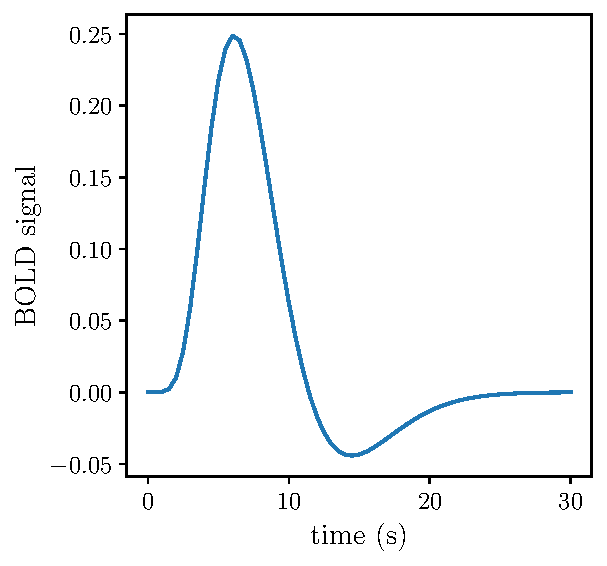
\includegraphics[scale=0.8]{figures/neuroscience/hrf.pdf}
  \caption{A model of the hemodynamic response function}
  \label{fig:hrf}
\end{figure}

Luckily, the shape of the hemodynamic response does not vary much across time
and therefore the BOLD signal is often seen as the result of the convolution of neural activation with the hemodynamic response.

\subsection{Spatial and temporal resolution of fMRI data}
The success of fMRI is due to its advantages compared to positron
emission topography (PET) that uses radioactive tracers to follow glucose or water levels.
While PET has a spatial resolution of a few
centimeters, fMRI has a spatial resolution of a few millimeters. As a result, a voxel in an fMRI image typically encompasses several hundreds thousands of neurons.
In addition, while taking an image with PET takes about a minute, it takes on the order of 2s to produce a full-brain fMRI image.
Lastly, fMRI is non-invasive and does involve being exposed to radioactive tracers as in PET.

\subsection{Experimental designs}
In \emph{resting state} fMRI, subjects are instructed to lie still in the scanner without further instruction.
This kind of data can be used to extract networks that highlight sets of regions that tend to co-activate.
This contrasts with \emph{task} fMRI, where subjects follow specific instructions.
In task fMRI, two types of experimental design are widespread.
Block designs are widespread designs particularly suited to modalities with low temporal resolutions (such as PET). In block designs, subjects are exposed to continuous stimuli that last of a rather long period of time before it switches to another.
This contrasts with event related designs that are only suited to modalities with a finer time resolution. In event related design, a sequence of short event are presented and separated by a time window (inter-stimulus interval).
When the inter-stimulus interval is shorter than the length of the hemodynamic response, we talk about ``fast'' even related designs.
Lastly, in \emph{naturalistic fMRI}, subjects are instructed to watch a movie
or listen to an audio track. These kinds of stimuli are called \emph{naturalistic stimuli} and constitue a middle ground between resting state and task fMRI as activations are time locked while the environment is not as controlled as in a typical task fMRI setting.
%
In this thesis, we use mostly \emph{naturalistic fMRI}, as one of our motivations is to propose a suitable framework to analyse such data.

\subsection{Preprocessing}
The fMRI signal is particularly noisy. Several techniques are used to reduce the noise and enhance the quality of the data.

\subsubsection{Distortion correction}
In the MRI scanner, a constant magnetic field is applied. However, in areas
where an air/tissue interface, the magnetic field is distorted leading to errors in
the localization of voxels near the sinus or ears. However, most scanners come
with a map quantifying the distance that each voxel has been shifted. By
inverting the map, one can try and recover the correct location of voxels.


\subsubsection{Slice timing correction}
Images are acquired in slices, a few slices at a time, so that different voxels are acquired at different times.
In order to correct for this effect, a reference slice is chosen and other slices are interpolated so that all the voxels can be considered to have been acquired at the same time. 

\subsubsection{Motion correction}
Head motion causes massive distortion of the signal. Such effects are corrected by
chosing a reference image and apply rigid body transformations so that other
images match the orientation and localization of the reference image. One also records estimated head movements parameters so that they can be regressed out. However, if the task is correlated with head motion, this regression can destroy signal.

\subsubsection{Spatial smoothing}
Spatial smoothing blurs the image by application of a Gaussian kernel with a given width (in mm). When the signal of interest has a large spatial extend, smoothing increases the signal to noise ratio. 
Smoothing is also used as a way to decrease between subject variability.
In our experiment, we usually don't apply smoothing in order to measure how our
methods are able to handle fined grained details. While there is currently no
consensus on smoothing, we observe that a smoothing of 3~mm generally improves
most analysis on fMRI data.

\subsubsection{Frequency filtering}
Heating of the scanner causes a low temporal frequency noise to appear. In order
to remove such noise, a high pass filtering is applied with a cut-off frequency
of $0.01 Hz$. Sometimes a low pass filter with a cut-off frequency of $0.1$ Hz is also used since artifacts induced by motion are usually of higher frequency than the signal of interest.

\subsubsection{Spatial normalization}
Each subject has a brain of different size and of different shape.
The goal of spatial normalization is to align the subjects in order to reduce anatomical variability.
The most widespread technique is to align all images on a template image. The
template image used is based on an atlas developed at the Montreal Neurological
Institute (MNI atlas) where 305 anatomical images were aligned, averaged and then re-aligned to the mean image based on an non-linear registration model.
An affine linear registration is applied, followed by non-linear deformation to better match brain shape. Typically, fMRI images of each subject are aligned on a high dimensional anatomical image of the same subject (this step is called \emph{coregistration}) and then the anatomical image is aligned to the MNI atlas. The two transformations are then composed to project fMRI data to the MNI space.

\subsubsection{Masking}
It is often the case that only a subpart of the brain is of interest. When this is the case, we use a mask to only keep the set of voxels corresponding to particular locations defined by the mask.

\subsubsection{Runs}
For the comfort of participants and to ensure their active participation, it is in general not possible to use the scanner without interruptions for more than 10 minutes.  When long acquisitions must be
performed they are split into short runs of approximately 10 minutes.


\subsection{Example of fMRI Datasets}
\label{srm:datasets:fmri}
In this subsection we provide examples of fMRI datasets. These datasets will be used to evaluate the methods developed in this thesis.
Datasets are preprocessed with FSL \url{http://fsl.fmrib.ox.ac.uk/fsl}  and SPM \url{https://www.fil.ion.ucl.ac.uk/spm/software} using slice timing correction, distortion correction spatial realignment, coregistration to the T1 image and affine transformation of the functional volumes to a template brain (MNI).
Using Nilearn \cite{abraham2014machine}, preprocessed data are masked (using a full brain mask available at
\url{http://cogspaces.github.io/assets/data/hcp_mask.nii.gz}), detrended and
standardized (so that any voxel's timecourse has zero mean and unit variance).
We also apply a high pass filter and a low pass filter with cut-off frequencies of 0.01 Hz and 0.1 Hz respectively).

In the \emph{SHERLOCK} dataset, 17 participants are watching "Sherlock" BBC TV show (episode 1). 
% 
These data are downloaded from \url{http://arks.princeton.edu/ark:/88435/dsp01nz8062179}. 
% 
Data were acquired using a 3T scanner with an isotropic spatial resolution of 3~mm. 
% 
More information including the preprocessing pipeline is available in \cite{sherlock}.
% 
Subject 5 is removed because of missing data, leaving us with 16 participants.
% 
Although SHERLOCK data contains originally only 1 run, we split it into 4 blocks of 395 timeframes and one block of 396 timeframes for the needs of our experiments. 

In the \emph{FORREST} dataset, 20 participants are listening to an audio version of the movie Forrest Gump.
% 
FORREST data are downloaded from OpenfMRI~\cite{poldrack2013toward}. 
% 
Data were acquired using a 7T scanner with an isotropic spatial resolution of 1 mm (see more details in \cite{hanke2014high}.
% 
More information about the forrest project can be found at \url{http://studyforrest.org}.
% 
Subject 10 and run 8 are discarded because of missing data.
% 
We therefore use full brain data of 19 subjects split in 7 runs of respectively 451, 441, 438, 488, 462, 439 and 542 timeframes.


In the fMRI \emph{CamCAN} dataset, 647 participants aged from 18 to 88 years are watching Alfred Hitchcock's "Bang! You're Dead" (edited so that it lasts only 8 minutes).
% 
CamCAN consists of data obtained from the CamCAN repository (available at \url{http://www.mrc-cbu.cam.ac.uk/datasets/camcan/}) (see \cite{taylor2017cambridge} and \cite{shafto2014cambridge}).
% 
We use all available subjects and runs yielding 647 participants and 1 run of 193 timeframes.


The \emph{RAIDERS} dataset reproduces the protocol described
in~\cite{haxby2011common}. 10 participants are watching the movie "Raiders
of the lost ark". This dataset pertains to the Individual Brain Charting
dataset~\cite{ibc, ibc2}.
% 
Data 
% 
We use full brain data of 10 subjects split in 9 runs of respectively 374, 297, 314, 379, 347, 346, 350, 353 and 211 timeframes.
%
Note that the Raiders dataset is different from the one used in~\cite{chen2015reduced}, as it involves different subjects, and because data were acquired at NeuroSpin using a 3T scanner with an isotropic spatial resolution of 1.5 mm.
The \emph{raiders-full} dataset~\cite{ibc, ibc2} is an extension of the \emph{raiders} dataset where the first two scenes of the movie are shown twice (130 mins).

The CLIPS dataset reproduces the protocol of original studies described in
\cite{nishimoto2011reconstructing} and \cite{huth2012continuous}. 10
participants are exposed to short clips. The data were acquired in 17 runs of 325 timeframes. 
%
The CLIPS dataset also pertains to the Individual Brain Charting dataset
(\cite{ibc, ibc2}).
%
At the time of writing, the CLIPS and RAIDERS dataset from the individual brain charting dataset \url{https://project.inria.fr/IBC/} are not yet public, but they will be in the future. Protocols on the visual stimuli presented are available in a dedicated repository on Github: \url{https://github.com/hbp-brain-charting/public_protocols}.

Unless stated otherwise we use spatially unsmoothed data, except for the
\emph{sherlock} dataset, for which the available data are already preprocessed
with a 6\,mm spatial smoothing. The temporal resolution or repetition time (TR) is 2s for all datasets except for the Sherlock dataset where the TR is 1.5s.
%

A summary about the size of each dataset is available in Table~\ref{tab:dataset_desc2}. Note in particular that all datasets have been resampled to 2mm isotropic resolution, leading to 212,445 voxels in the brain mask.
\begin{table}
	\begin{tabular}{|c|c|c|c|c|}
		\hline
		\textbf{Dataset} & \textbf{Subjects} & \textbf{Runs} & \textbf{Average run} & \textbf{Voxels} \\
                     && & \textbf{length} & \textbf{(per subject)} \\
                     && & \textbf{(in timeframes)} &  \\
                     &$m$& $ $ & $n$ &$v$  \\
		\hline
		CLIPS & 10 & 17 & 325 & 212445\\ 
		\hline
		SHERLOCK & 16 & 5 & 395 & 212445 \\ 
		\hline
		RAIDERS & 10 & 9 & 330 & 212445 \\
		\hline 
		FORREST & 19 & 7 & 465 & 212445\\
		\hline
		CamCAN & 647 & 1 & 193 & 212445 \\
		\hline
	\end{tabular}
  \caption{\textbf{Datasets description}}
  \label{tab:dataset_desc2}
\end{table}

\subsection{An example of univariate analysis: analyzing task fMRI data via the general linear model}
\label{sec:glm}
In this section, we describe a framework successfully applied to identify brain regions involved in specific tasks: the general linear model
(GLM)~\cite{friston1995analysis}. We refer the reader to
Poline~\cite{poline2012general} for a more detailed description of the model and only cover here what we consider to be the most important parts.

We associate to each image $t$ a set of numbers $\sbb(t)$ that describe the experiment and
nuisance parameters.
For instance, in an experiment where the subject is either asked to listening a
sentence or reading a sentence we could have the association: $\sbb(t) = (\phi(t), \tau(t), x(t), y(t),
z(t))$ where $\phi(t)=1$ if the subject is reading a sentence and $0$ otherwise, $\tau(t)=1$
if the subject is listening to a sentence and $0$ otherwise and  $x(t), y(t), z(t)$ describe the
position of the head. While $\phi$ and $\tau$ describe the experiment, $x, y, z$
describe nuisance parameters.
Note that in practice we use many more nuisance regressors, such
as parameters describing the rotation of the head, heartbeats, respiration
rhythm and really any other parameter that might introduce artifacts. We also
usually convolve the regressors describing the experiment with the hemodynamic
function so that they are closer to the actual brain response and sometimes also its derivative to account for small temporal deviations from our model of hemodynamic response.
We call $S \in \RR^k, n}$ the \emph{design matrix} (in standard textbooks it is
usually called $X$ but in this thesis we use $X$ for the data) such that column
$t$ of $S$ is given by $\sbb(t)$.
Then, the general linear model sees the data of one subject $X \in \RR^{v \times n}$ as a linear combination of the
design matrix $S$ with additive noise $N$.
\begin{align}
X = A S + N
\end{align}
where $A \in \RR^{v \times k}$ contains $k$ spatial maps in the sense that column $j$
of $A$ can be plotted as a brain image representing the localization of activity
described by the row $j$ of $S$.
The noise is often assumed to be Gaussian with unit variance so that $A$ can be obtained as the
result of a linear regression. Another common hypothesis is to assume temporal
correlation of the noise in the form of an AR-1 process. In this case, we 
consider instead the data $XB$ where $B \in \RR^{n \times n}$ is chosen so that the
noise $BN$ has no temporal correlation allowing us to perform linear regression.

The result of the GLM procedure is often given by \emph{contrasts maps} where
the spatial maps corresponding to conditions of interest are subtracted.
In our reading versus listening example, we would typically display the first column of
$A$ (that corresponds to $\phi$ which describes the activation related to
reading a sentence) minus
the second column of $A$ (that corresponds to $\tau$ which describes the
activation related to listening to a sentence). An example of ``reading versus listening contrast is displayed in
Figure~\ref{fig:ibc_contrast}.

\begin{figure}
  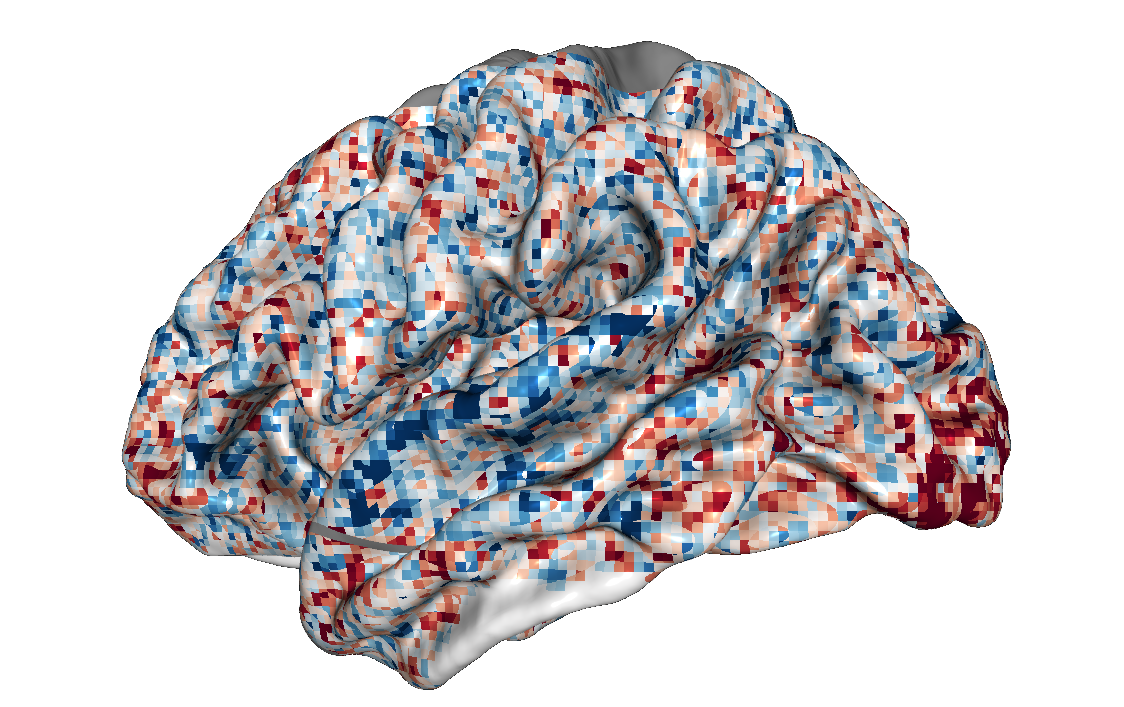
\includegraphics[scale=0.3]{figures/neuroscience/spatial_map.png}
  \caption{Contrast ``sentence listening versus sentence reading'' computed from the fMRI data of one
    subject in the IBC dataset~\cite{ibc, ibc2}. This contrast was downloaded
    from neurovault~\cite{gorgolewski2015neurovault} (collection 2138 subject 1 session 0) .}
  \label{fig:ibc_contrast}
\end{figure}


While in this thesis, we always work with unthresholded contrast maps like the one in Figure~\ref{fig:hcp_contrast}, contrast maps
are usually thresholded to keep only activity that is significantly
different from zero.
The GLM model is called univariate since interactions between voxels are not
modeled.
Univariate methods are often criticized for their inability to
capture well correlations and interactions between brain-wide measurements.
This makes it difficult to precisely locate brain functions from brain maps. An approach to overcome this issue is to train classifiers to \emph{decode} brain maps, i.e to discriminate between different stimulus of task
types~\cite{shirer_decoding_2012,varoquaux_how_2014,loula_decoding_2018}. When linear classifiers are used, the weights of this classifiers localize the brain functions.
This approach can be more powerful, as classifiers take correlations between
voxels into account. Decoding is also popular for individual imaging-based diagnosis.

\section{Magneto electro encephalography (MEG)}
Most material in this section is inspired from the book of Riitta Hari and Aina
Puce~\cite{hari2017meg}.

\subsection{Principle of MEG}
When a neuron fires, it emits a current that generates a magnetic field. By
recording the magnetic field close to the skull, we gain insight on neural
activity.

A limiting factor is that the magnetic fields induced by neuronal currents are
extremely weak (on the order of $10 fT$) which is much lower than the ambient magnetic noise ($10^8 fT$). Therefore recordings are performed in a shielded room and extremely sensitive magnetometers are used.
The best current tools can measure the magnetic filed generated by approximately 50~000 neurons oriented in the same direction.

MEG recording device also include gradiometers in addition to magnetometers.
These are sensitive to the local variations of the magnetic field. However in our experiments, we only use the magnetometers data.

MEG has a temporal resolution on the order of the ms which is essentially the same as electroencephalography (EEG). This is much better than fMRI. The spatial
resolution is similar to that of EEG and is on the order of the centimeter.
In general the brain sources are slightly better localized in MEG since the
magnetic field is not affected by changes in conductivity in the head.


\subsection{Solving the inverse problem}
In order to locate activation from the brain measurements, we need to solve an inverse problem: what kind of sources can generate the magnetic field we
observe ? This section gives an overview of the sLoreta
method~\cite{pascual2002standardized} and is strongly inspired from the tutorial
of the authors~\cite{pascual2007discrete}.

From a vector describing the 3D current density inside the brain $\jb \in \RR^{3 \times v}$
($v$ is the number of voxels) we
can predict the magnetic field recorded by the sensors $\bb \in \RR^p$ ($p$ is the number of sensors) provided
we know how the magnetic field propagates through the brain by using Maxwell's
equation. This is called the \emph{forward model}. Models describing the
geometry of the head (head models) are used to provide an approximate solution for the forward model.
We have therefore
\begin{align}
  \bb = K \jb
  \label{eq:maxwell}
\end{align}
where $K \in \RR^{p \times 3v}$ is given by the head model.
$K$ can be seen as $K  = [K_1 \dots K_{v}]$ where $K_i \in \RR^{p \times 3}$ describes how voxel $i$ contributes to the measured magnetic field $\bb$.

Note that if $\bb$ and $K$ are given there is an infinite number of possible
$\jb$ so the inverse problem must be regularized in order to select a solution among all possible ones.
A common parametrization is to assume that:
\begin{align}
\jb(K_i) = (K_i^{\top} C K_i) \bb
\end{align}
for a symmetric matrix $C \in \RR^{p \times p}$ and $\jb(K_i)$ describes the current at voxel $i$.
In sLoreta, we have $C = (K K^{\top} + \alpha I)^{\dagger}$ where $\dagger$
represents Moore's pseudo inverse, $I$ is the identity matrix and $\alpha$ is an hyperparameter. 

Taking a point wise source $\ab \in \RR^{3}$ at voxel $j$
equation~\eqref{eq:maxwell} yields $\bb = K_j \ab$.
Then, $\| \jb(K_i) \|^2$ is maximum at $K_i=K_j$ showing that the method can correctly recover point sources.

\subsection{Preprocessing steps}
This section is inspired from the preprocessing recommandations
in~\cite{jas2018reproducible} and the book of Riitta Hari and Aina
Puce~\cite{hari2017meg}. 

\subsubsection{Temporal filtering}
Temporal filtering is usually done by analogous filtering using a wide range of
frequency (typically from $0.01 Hz$ to $200Hz$.
A digital filtering is usually applied afterwards. A low-pass filtering with
cut-off frequency at $40 Hz$ is valuable as it is below the line frequency. It
also removes some of the artifacts due to eye movements although subjects are
often asked to fix a cross on a screen while scanning.

\subsubsection{Independent component analysis}
Independent component analysis (ICA) can be used to isolate artifacts due to
heart beating or muscle contraction. As will be seen in section~\ref{sec:ica}.
ICA extracts independent components from the data. The data can be cleaned by
removing components corresponding to artifacts.

\subsubsection{Maxwell filtering}
Maxwell filtering also called signal space separation
(SSS)~\cite{taulu2006spatiotemporal} identifies the contributions of the
magnetic field from brain sources outside the brain and removes it.
This decreases the effect of outside noise and even allows to scan subjects with
implemented stimulators.


\subsection{Experimental designs}
Two kinds of response are generally studied in MEG: \emph{evoked response} and
\emph{event related} response.
The evoked response is observed when the subject is exposed to a short stimuli.
We typically repeat the experiment multiple times and average the subject
response over trials.
Another technique is to average signal with respect to some event such as eye
movement or utterance of a word. The recovered signal is then called
event-related response.

\subsection{MEG datasets}
\label{sec:meg:datasets}
In this section, we give examples of MEG datasets. These examples are used in
the rest of the thesis to evaluate the methods developed.

The \emph{Sinusoidal Phantom MEG} dataset uses data collected with a realistic head phantom, which is a plastic device mimicking real electrical brain components.
% 
Eight current dipoles positioned at different locations can be switched on or off.
% 
We only consider the 102 magnetometers.
% 
An epoch corresponds to 3\,s of MEG signals where a dipole is switched on for 0.4\,s with an oscillation at 20\,Hz and a peak-to-peak amplitude of 200\,nAm.
% 
We have access to $100$ epochs per dipole.
%
Maxwell filtering was applied on the data and a low pass filter with cut-off
frequency at 40 Hz.

The \emph{Elekta Phantom MEG} dataset also uses data collected with a realistic
head phantom and is available as part of the Brainstorm
application~\cite{tadel2011brainstorm}.
This dataset involves 32 different dipole locations. Like in the
\emph{sinusoidal phantom} we only
consider the 102 magnetometers and apply Maxwell filtering and a low pass filter
with cut-off 40 Hz. The dipoles emit a signal at either a strong, medium or low
amplitude yielding 3 datasets.
We use the dataset where the emitted signal is very strong to recover the true signal
by performing a PCA with 1 component.
Then we work with the dataset where the emitted signal is the weakest.
Each epoch corresponds to 301 samples and 20 epochs are available in total.

The \emph{CamCAN} dataset~\cite{shafto2014cambridge}
contains the MEG data of 647 different
subjects exposed to an audio-visual stimuli. More precisely, subjects are presented simultaneously an
auditory stimuli lasting 300ms at frequency 300, 600 or 1200 Hz  and a
checkerboard pattern lasting 34ms. 120 trials are available.


\chapter{Review of selected unsupervised methods popular in neuroimaging studies}
\label{ch:review}
When exposed to naturalistic stimuli (e.g. movie watching or simulated driving), subjects' experience is closer to their every-day life than with classical
psychological experiments.
% 
This makes naturalistic paradigms an attractive class of
stimulation protocols for brain imaging.
%
However, such stimulations are difficult to model, therefore the statistical analysis of the data using supervised regression-based approaches is challenging.
This has motivated the use of unsupervised learning methods that do not make
assumptions about what triggers brain activations in the presented stimuli.

In this chapter, we first present \emph{independent component analysis} (ICA), a widely used
unsupervised method for neuroimaging studies routinely applied on individual
subject electroencephalography (EEG)~\cite{makeig1996independent},
magnetoencephalography (MEG)~\cite{vigario1998independent} or functional MRI
(fMRI)~\cite{mckeown1998independent} data, then we review \emph{multiview} unsupervised 
techniques that leverage the availability of data from multiple subjects
performing the same experiments. 

\section{Independent component analysis}
\label{sec:ica}
Independent component analysis (ICA) models a set of signals as the product of a \emph{mixing matrix} and a
\emph{component} matrix containing independent components. As will be seen in this
section, the required assumptions on the independent components to guarantee
identifiability are rather weak, making ICA a method of choice to analyze the
data of subjects exposed to a stimulus that is difficult to quantify.

ICA is applied to fMRI data to analyze resting state
data~\cite{beckmann2005investigations} or when subjects are
exposed to natural~\cite{malinen2007towards}~\cite{bartels2005brain} or complex stimuli~\cite{calhoun2002different}. 
In M/EEG processing, it is widely used to isolate acquisitions artifacts from neural signal~\cite{jung1998extended}, and to identify brain components of interest~\cite{vigario2000independent, delorme2012independent}.

In neuroscience, the number $k$ of components is typically much lower than the number $v$
of available observations. We are therefore in an overcomplete setting.
However in ICA, it is assumed the number of observations is equal to the number
of components. Therefore, a
typical pre-processing step is to reduce the dimension. We therefore first
present principal component analysis which is the standard method to perform
dimension reduction in this context.

\subsection{Principal component analysis (PCA)}
Let us assume our data are given by a random vector $\xb \in \RR^{v}$. The data
are centered ($\EE[\xb] = 0$). Principal component analysis (PCA) gives an orthonormal familly of $p$ vectors $R \in \RR^{v \times p}$ such that projecting our data onto this family
using $R R^{\top} \xb$ does not yield a large reconstruction error in Frobenius
norm.
The corresponding optimization problem is given by:
\begin{align}
  &\argmin_{R} \|\xb - R R^{\top} \xb \|^2 \\
  &=\argmin_{R} \trace(  \xb^{\top}(I - R R^{\top}) (I - R R^{\top}) \xb\|^2 \\
  &= \argmin_{R} \|\xb \|^2 - \|R^{\top} \xb \|^2 \\
  &= \argmax_{R} \|R^{\top} \xb \|^2 \\
  &= \argmax_{R} \trace(R^{\top} \VV[\xb] R)
\end{align}
Therefore the matrix $R$ is just given by the first $p$ eigenvectors of
$\VV[\xb]$. In practice the observed data can be represented as a matrix $X \in \RR^{v, n}$,
from which one can compute an empirical estimate of the covariance by $\frac1{n}X X^{\top}$.
%
However, such an estimate is not practical in high dimension: $v$ is very
large and therefore $XX^{\top}$ is a prohibitively large matrix.

Therefore, we rely instead of the singular value decomposition of $X$:
\begin{align}
X= U D V
\end{align}
  where $U \in \RR^{v \times t}$ is an orthogonal matrix ($U^{\top} U
= I_t$) of
\emph{left-singular vectors}, $D \in \RR^{t}$ is a positive diagonal matrix of
singular values and $V \in \RR^{t \times t}$ is an orthogonal matrix of
\emph{right-singular vectors}.
%
Every matrix has a singular value decomposition and this
decomposition is unique up to reordering of the singular vectors (and
corresponding permutations of the left/right singular vectors) and sign-flips of
the left and right singular vectors.

Let $X = UDV$ be a singular value decomposition of $X$, we have $XX^{\top}= U
D^2 U^{\top}$ and therefore the left-singular vectors $U_p$ corresponding to the
largest $p$ singular values of $X$ yield  the $p$ largest eigenvectors of
$XX^{\top}$.
Therefore $R = U_p$.

Sometimes the PCA includes whitening $R = U_p D_p^{-1}$ where $D_p$ contains the
 $p$ largest singular values of $X$ so that projected data are
uncorrelated (but $R$ is no longer orthonormal). In this paper what we call PCA
does not include signal whitening.

After the data are reduced such that the number of observations are identical to
the number of components, we can perform independent component analysis (ICA).
ICA can exploit a number of different properties of the signal. Most ICA
algorithms use non-gaussianity of the data to extract relevant components so we
focus next on non-Gaussian ICA.

\subsection{Non Gaussian ICA}
ICA sees the data $\xb \in \RR^p$ as a linear mixtures of components $\sbb \in \RR^p$.
Data are therefore modeled as:
\begin{align}
  \xb = A \sbb
\end{align}
where $A$ is the unmixing matrix and $\sbb$ have a non-Gausian distribution.
Without loss of generality, the data $\xb$ are assumed centered ($\EE[\xb] = 0$).
This section relies heavily on the ICA review~\cite{hyvarinen2000independent}
and on~\cite{cardoso1997infomax}.

\subsubsection{Identifiability}
It is easily seen that if $\sbb$ is non-Gaussian, so is $P \sbb$ where  $P$ is a
sign and permutation matrix.
Therefore if $\xb = A \sbb$, take $A' = AP^{\top}$ and $\sbb'=P\sbb$ and we have
$\xb = A' \sbb'$.
In other words, there exists a permutation and scaling indeterminacy.
\tetxbf{XXX sign or scaling ? There seems to be a confusion througgout the paragraph}

Therefore, we can assume without loss of generality that $\sbb$ has unit variance ($\VV[\sbb] = I$).
If we whiten the data by applying a matrix $H$ such that $\VV[H \xb] = I_p$ we have $H \xb = \tilde{A} \sbb$ where $\tilde{A} = HA$. $\VV[H \xb] = 1$ implies $\tilde{A}^{\top} \tilde{A} = I$ so without loss of generality we can assume that $\xb$ has unit variance and that $A$ is orthogonal. 

We now show that the previously described scale and permutation
indeterminacies are the only one.
Let us assume that there exists two mixing matrices $A_1$ and $A_2$ such that
$\xb = A_1 \sbb_1$ and $\xb = A_2 \sbb_2$ with $A_1$ and $A_2$ orthogonal. Then $\sbb_1 = O \sbb_2$ where $O = A_1^{\top} A_2 \sbb_2$.
The following theorem in~\cite{comon1994independent}
shows that $O$ can only be a scale and permutation matrix.
\begin{theorem}
  Let $\sbb_2$  be a  vector  with  independent 
  components, of   which  at  most  one  is  Gaussian,  and whose  densities
  are  not  reduced  to  a  point-like  mass. Let $O$ be an orthogonal matrix
  and $\sbb$ such that $\sbb = O \sbb_2$.
  Then, $\sbb$ has independent component if and only if $O$ is a scale and
  permutation matrix.
\end{theorem}

As a result, if we assume that at most one component is Gaussian, ICA is identifiable up to a scale and permutation indeterminacy.

\subsubsection{Infomax: Maximum likelihood estimation}
Infomax is introduced in~\cite{bell1995information} in the context of source
separation as maximizing the entropy of $g(W \xb) = g_i(\wb_i \xb)$ where  $g_i$
is differentiable, strictly increasing function with value in $]0, 1[$. As shown
in~\cite{cois1997infomax}, this is equivalent to
maximum likelihood where component $i$ is assumed to have $g_i$ as its
cumulative distribution function.

Assume for simplicity that the components have the same density $\delta$, denoting $f(x) =
-\log(\delta(x))$ and $f(\xb) = \sum_{i=1}^m f(x_i)$ for $\xb \in
\RR^m$ the negative log-likelihood is given by:
\begin{align}
  \loss &= -l(\xb, \theta) = - \log(p(\xb)) \\
        &= -\log(|W|) - \log(\delta(W \xb)) \\
  &= -\log(|W|) + f(W \xb)
\end{align}
where we used the change of variable $\sbb = W \xb$.

\subsubsection{Optimizing the maximum likelihood: relative gradient, Hessian and approximations}
\label{sec:opt:likelihood:relativegradient}
The matrix $W$ needs to be invertible. In practice, if the constraint is not
enforced, we could see numerical instabilities appear.
A simple rule that preserve the inversibility of $W$ is to use updates of the
form:
\begin{align}
  W \leftarrow (I + \alpha D)W \label{eq:mult:update}
\end{align}
where $\alpha$ is a small step-size and $D$ is a direction to be found.
Following the same reasonning as in section~\ref{sec:gd}, we assume a small step-size
and write at first order:
\begin{align}
  \argmin_{D, \|D\|=1} \loss((I + \alpha D)W) &= \argmin_{D, \|D\|=1} \loss(W) + \langle \partialfrac{W}{f(W)} | \alpha D W \rangle \\
                                              &= \argmin_{D, \|D\|=1} \loss(W) + \langle \partialfrac{W}{f(W)} W^{\top} | \alpha D \rangle \\
                                              &= -\frac{\partialfrac{W}{f(W)} W^{\top}}{\|\partialfrac{W}{f(W)} W^{\top} \|}
\end{align}
The updates are therefore given by  $W \leftarrow (I - \alpha G)W$ where $G = \partialfrac{W}{f(W)}
  W^{\top}$ is called the \emph{relative
  gradient}~\cite{cardoso1996equivariant}.
Second order extensions of the method are obtained by following the steps in
section~\ref{sec:qn}. The corresponding Hessian is called the \emph{relative
  Hessian}.
As a side note, the relative gradient coincides with the natural
gradient~\cite{amari1999natural} that exploits the property of the statistical model. \textbf{XXX Please clarify what yoy mean here}


Let us follow~\cite{ablin2018faster} and use a quasi-Newton algorithm to minimize the likelihood.
The relative gradient and Hessian of $\loss$ are given by:
\begin{align}
  G = f'(\yb) \yb^{\top} - I_p,
\end{align}
where $\yb = W \xb$ and $f'(\yb) = \partialfrac{f(\yb)}{\yb}$ \textbf{XXX the inverse ?}
and
\begin{align}
  H_{abcd} =  \delta_{ad}\delta_{bc} + \delta_{ac} f''(y_a)y_by_d
\end{align}

Following~\cite{ablin2018faster}, we can approximate the Hessian by
\begin{align}
  \tilde{H}_{abcd} = \delta_{ad} \delta_{bc} + \delta_{ac} \delta_{bd} \Gamma_{ab}
\end{align}
where $\Gamma_{ab} = f''(y_a) y_b^2$.
The approximation is exact when the true unmixing matrix is found since $\EE[s_b s_d] =  s_b^2\delta_{bd}$.

The updates are then given by:
\begin{align}
  W \leftarrow (I - \alpha \tilde{H}^{-1} G) W
\end{align}

Note the abuse of notation here. In the update formula, we actually mean
$\EE[\tilde{H}]$ and $\EE[G]$,
instead of $\tilde{H}$ and $G$.
In practice, these expectations are replaced by empirical expectations. We often do such abuse in the rest of the thesis when it is clear from the context whether we mean random variables or their (empirical) expectation. 

Note that the term $\tilde{H}^{-1} G$ is particularly easy to compute. Indeed we
have:
\begin{align}
[\tilde{H}^{-1} G]_{ab} = \frac{\Gamma_{ba} G_{ab} - G_{ba}}{\Gamma_{ba}
  \Gamma_{ab} - 1}
\end{align}

\subsubsection{Robustness to density mismatch}
In practice, we observe that sometimes, the quasi-Newton algorithm described in
the previous section fails to recover the true mixing matrix. This happens when the
sources used in the model are too far from the actual  generating sources.
%
In this section, we explain
why this happens and derive stability conditions. This follows the work done in~\cite{cardoso1998blind}.

When the density of the sources corresponds to the one used in the model, one
recovers the correct unmixing matrices via the maximum likelihood estimate in the
limit of large samples. This comes from the consistency of maximum likelihood
estimators.
When this is not the case, a mismatch appears which can be quantified. Let us
denote $\xb^*$ the true data. As highlighted in~\eqref{kl-likelihood} the expected
negative log-likelihood coincides, up to a constant, with the KL divergence between the true
distribution of the data and the distribution of the data as hypothesized in the
model:
\begin{align}
  &-l(\theta) \\
  &=  D_{KL}(p(\xb^*), p(W^{-1} \sbb)) \\
             &=  D_{KL}(p(W\xb^*), p(\sbb)) \\
             &=  D_{KL}(p(W \xb^*), \prod_i p_i(\wb_i\xb^*)) + D_{KL}(\prod_i p_i(\wb_i\xb^*), p(\sbb)) \\
             &=  D_{KL}(p(W \xb^*), \prod_i p_i(\wb_i\xb^*)) + D_{KL}(\prod_i p_i(\wb_i\xb^*), \prod_i p_i(s_i)) \\
\end{align}
where the first equality comes from the invariance of the KL divergence and we
denote $\prod_i p_i(x_i)$ the product of the marginal densities of $\xb$.

The first term in the last equality is the mutual information. It quantifies the
independence of unmixed data $W \xb$. The second term quantifies the mismatch
between the assumed distribution of the components and the marginals of unmixed data.
Therefore if the assumed components are too far from the true components, the
recovered unmixing matrices may be far from the true ones.


Looking at the relative gradient $G$, we see that if components are truly
independent, the true unmixing matrix will be a stationary point of the loss up
to a scaling: $G(\Lambda A^{-1})=0$ where $\Lambda=\diag(\lambda_1 \dots \lambda_p)$.
However, in order for the quasi-Newton to reach this point, it must be a local
minimum (the Hessian must be definite positive). 

Let us therefore consider the Hessian $H$ at point $W = \Lambda A^{-1}$ where
$\Lambda$ is chosen such that $G = 0$. The unmixed data $\yb = W \xb$ are independent and
therefore, we have $\tilde{H} = H$.
For any matrix $M$:
\begin{align}(\tilde{H} M)_{ab} = M_{ba} + M_{ab} f''(y_a)y_b^2.
\end{align}
So $\tilde{H}$ is block diagonal with blocks of size either 1 or 2.
The blocks of size 1 are given by :
\begin{align}
  1 + f''(y_a) y_a^2
  s_a^2
\end{align}
and the blocks of size
two are given by the matrix
\begin{align}
                              \begin{bmatrix} f''(y_a) y_b^2
  & 1 \\ 1 &
  f''(y_b)y_a^2 \end{bmatrix}
\end{align}
Therefore the conditions for stability are given by:
\begin{align}
  \forall a, b, a \neq b, \enspace \left(f''(y_a) y_a^2 \right) \left(f''(y_b)  y_b^2 \right) > 1
\end{align}

When the conditions are satisfied, the quasi-Newton algorithms will recover the
true unmixing matrices if initialized close to a solution. In practice, this
method recovers the correct unmixing matrices in a wide variety of cases.

\subsection{A variation : non-stationary ICA and joint diagonalization}
Up to now we have assumed that samples were independent an identically distributed. In non-stationary ICA, samples are no longer identically distributed as the distribution can vary over time.
This section follows the work in~\cite{pham2001blind}.
The components are assumed to be Gaussian with a variance that varies between
samples but is assumed to be piece-wise constant $\Sigma_t = \Sigma_k$ for $t \in
T_k$ where $(T_k)_k$ is a partition of $[1, 2, \dots, n]$ and $\Sigma_k$ is a
positive diagonal matrix.

The log-likelihood is given by:
\begin{align}  
  \loss &= -\log(|W|)  + \frac1{n} \sum_k \big( \frac12 \sum_{i \in T_k}\|\Sigma_k^{-\frac12} W \xb^k_i \|^2 + \frac12 \log(|\Sigma_k|) \big)
\end{align}
\textbf{XXX unsure about the sign}
Denoting $C_k = \sum_{i \in T_k} \xb_i^k (\xb_i^k)^{\top}$ we have 

\begin{align}  
  \loss &= -\log(|W|)  + \frac1{n} \sum_k \big( \frac1{2} \trace(\Sigma_k^{-1} W C_k W^{\top}) + \frac12 \log(|\Sigma_k|) \big)
\end{align}
Minimizing $\loss$ with respect to $\sigma_k^2$ yields $\Sigma_k = \diag(W C_k
W^{\top})$ and therefore up to a constant:
\begin{align}  
  \loss &= -\log(|W|)  + \frac1{n} \sum_k \big(\frac12 \log(|\diag(W C_k W^{\top})|) \big)
\end{align}
which can be rewritten:
\begin{align}  
  \loss &=\frac1{2n} \sum_k \big(\frac{\log(|\diag(W C_k W^{\top})|)}{\log(W C_k W^{\top})} \big)
\end{align}

$\loss$ is a joint diagonalization criterion. The optimal $W$ can be found via a
quasi-Newton method very similar to the one we used for non-Gaussian
ICA~\cite{ablin2018beyond} however, performing ICA via joint diagonalization is
in principle much faster than using non-Gaussian ICA.

\section{Analysis of MultiView data}
In this section, we present multiview unsupervised techniques suited to
analyze the data of multiple subjects exposed to the same complex stimuli. Such
techniques assume some similarity between the data of different subjects. This
assumption can be justified by the findings of \cite{hasson2004intersubject} showing that brains exposed to the same natural stimuli exhibit synchronous activity.
The task of finding common patterns or responses that are shared between
subjects is called \emph{shared response modeling}.

In the general linear model presented in
section~\ref{sec:glm}, the shared response is assumed to be known. Therefore,
multiple subjects can be studied separately assuming that the data of different
subjects are independent given the shared response.
In the unsupervised setting it may not be so straightforward to deal with
multiple subjects and therefore many different
methods for data-driven multivariate analysis of neuroimaging group studies
have been proposed.
We summarize the characteristics of some of the most commonly used ones.


\subsection{Multiset canonical correlation analysis}
\label{sec:mcca}
Canonical correlation analysis is initially designed to find a linear
combination that maximizes the correlation between two datasets.
The extension to more than two datasets is ambiguous, and many
different generalized CCA methods have been proposed. \cite{kettenring1971canonical} introduces 6 objective functions that reduce to CCA when $m=2$ and \cite{nielsen2002multiset} considered 4 different possible constrains leading to 24 different formulations of Multiset CCA.

In this section, we present the formulation refered to
in~\cite{nielsen2002multiset} as SUMCORR with constraint 4 which is one of the
fastest to fit.

Let us consider $\xb_1, \dots, \xb_m$, $m$ datasets and consider the following (SUMCORR)
objective:
\begin{align}
  \max_{\ab_1 \in \RR^{v}, \dots, \ab_m \in \RR^{v}} \sum_{i=1}^m \sum_{j=1}^m \langle \ab_i | X_i X_j^{\top} \ab_j \rangle
\end{align}
This objective can be arbitrarily large if not constrained. Constraint 4 is
given by:
\begin{align}
  \sum_{i=1}^m \langle \ab_i X_i X_i^{\top} \ab_i \rangle = 1
\end{align}

The Lagrangian is given by:
\begin{align}
  \sum_{i=1}^m \sum_{j=1}^m \langle \ab_i | X_i X_j^{\top} \ab_j \rangle - \lambda (\sum_{i=1}^m \langle \ab_i X_i X_i^{\top} \ab_i \rangle - 1)
\end{align}

Taking the gradient with respect to $\ab_i$ we obtain
\begin{align}
  \sum_{j=1}^m X_i X_j^{\top} \ab_j = \lambda X_i X_i^{\top} \ab_i
\end{align}

This is a generalized eigenvalue problem of the form $C \ab = \lambda D \ab$
where $C$ is a block matrix where block $i,j$ is given by $X_i X_j^{\top}$, 
$D$ is the block diagonal matrix formed by the block $i, i$ of $C$ and $\ab \in
\RR^{mv}$ yields the dataset specific projections vectors: $\ab = \begin{bmatrix} \ab_1 \\ \cdots \\
  \ab_m \end{bmatrix}$.

    The leading eigenvector correspond to the first canonical vectors. The
    second canonical vectors is given by the second eigenvalues and so on. They
    are orthogonal for the scalar product: $\langle \ab, \bb  \rangle_D =
    \langle \ab, D \bb  \rangle$.

  
\subsection{Group independent component analysis}
\label{sec:groupica}
Given the success of ICA in analyzing the data of one subject. It is natural to
look for extensions of ICA in a multiview setting.
Several works assume that the subjects share a common mixing matrix, but with different components~\cite{pfister2019robustifying}~\cite{svensen2002ica}.
% 
Instead, we focus on models where the subjects share a common components matrix, but have different mixing matrices.

\subsubsection{CanICA and ConcatICA}
\label{sec:canicaandconcatica}
In the single subject setting, we reduce the data (for example using PCA) and apply ICA on
reduced data. Therefore a natural framework to perform group ICA is to first aggregate the
data of individual subjects into a single dataset, often resorting to dimension
reduction technique and then apply off-the-shelf ICA on the aggregated dataset.
When PCA is used to aggregate the data, the method is referred to as
ConcatICA~\cite{calhoun2001method}. An alternative is to use multiset canonical
correlation analysis (CCA) leading to a method called CanICA~\cite{varoquaux2009canica}.

This framework has the advantage of being simple and
straightforward to implement since it resorts to customary single-subject
ICA method.

When datasets are high-dimensional, a three steps procedure is often used: first
dimensionality reduction is performed on data of each subject  separately; then
the reduced data are merged into a common representation; finally, an ICA
algorithm is applied for shared components extraction.

CanICA and ConcatICA are popular methods for fMRI~\cite{calhoun2009review} and EEG~\cite{eichele2011eegift} group studies. These methods directly recover only group level, shared components; when individual components are needed, additional steps are required (back-projection \cite{calhoun2001method} or dual-regression \cite{beckmann2009group}).
% 

\subsubsection{Likelihood based method}
\label{sec:guo}
While CanICA and ConcatICA are simple to implement and very fast to fit, they do
not rely on maximum likelihood estimators. Therefore they do not benefit of
advantages of such estimators such as asymptotic efficiency.

The model of~\cite{guo2008unified} considers the very general model $\xb_i = A_i\sbb + \nb_i$, where the noise covariance can be learned from the data. 
\textbf{XXX Noisy ICA then ?}
In~\cite{guo2008unified}, each sources is assumed to be a mixture of Gaussians
$p(s_j) = \sum_{z=1}^q \Ncal(\mu_{zj}, \sigma_{zj})$.
where parameters of the Gaussian mixtures are learned. The fact that these
parameters are learned, making the E-step impossible to compute in closed form. In
addition, the
approximate E-step described in~\cite{guo2008unified} involves at each iteration
a costly sum where the number of terms is $q^p$ making their algorithm
intractable when the number of components $p$ is larger than $20$ even if the
number of Gaussian mixtures is as small as $q=2$. 

In this section, we assume that the parameters of the Gaussian mixture are
known, take $q=2$ and assume the same noise variance $\sigma$ for all subjects and all
components. In this
simplified setting, we will show that the E-step is in closed form but involves
a large sum with $q^p$ terms.

Note that in this setting the problem can be treated as a single subject noisy
ICA problem where $A = \begin{bmatrix} A_1 \\ \vdots  \\ A_m \end{bmatrix}$,
$\xb = \begin{bmatrix} \xb_1 \\ \vdots  \\ \xb_m \end{bmatrix}$ and $\nb
= \begin{bmatrix} \nb_1 \\ \vdots  \\ \nb_m \end{bmatrix}$. This showcases the
strong link between~\cite{guo2008unified} and~\cite{moulines1997maximum}.

We assume the following Gaussian mixture for each component $s_j$.
\begin{align}
  &p(s_j) = \frac12 \sum_{\alpha_j \in \{\frac12, \frac32\}} p(s_j | \alpha_j) \\
  &p(s_j | \alpha_j) = \mathcal{N}( s_j; 0, \alpha_j),
\end{align}
\textbf{XXX I am confused. Why do you introduce these values $1/2$ and $3/2$ ? None of your statements here depends on that choice...}
where $\alpha_j$ can be seen as a random variable that take its value in $\{ \frac12,
\frac32 \}$  with equal probability. We call $\alphab$ the random vector with
independent coordinates such that coordinate $j$ is given by $\alpha_j$.

Following a similar direction as~\cite{moulines1997maximum} we can write:
\begin{align}
  &p(\xb, \sbb, \alphab) \\
  &= p(\xb | \sbb) p(\sbb|\alphab)p(\alphab) \\
                        &= \Ncal(\xb; A\sbb, \sigma^2 I_p)\mathcal{N}( \sbb; 0, \diag(\alphab)) \frac1{2^p} \\
  &\propto \frac{\exp\big(-\frac12(\frac1{ \sigma^2}\|\xb - A\sbb \|^2 + \langle \sbb , \diag(\alphab)^{-1} \sbb\rangle)\big)}{(|\sigma^2 I_p| |\diag(\alphab)|)^{\frac12}}  \\
  &= \frac{\exp\big(-\frac12(\frac1{ \sigma^2}(\|\xb \|^2 - 2 \langle \xb, A \sbb \rangle + \|A \sbb \|^2)  + \langle \sbb , \diag(\alphab)^{-1} \sbb\rangle) \big)}{(|\sigma^2 I_p| |\diag(\alphab)|)^{\frac12}} \\
  &\propto \frac{\exp\big(-\frac12( \langle \sbb - \mu_{\alphab}, V_{\alphab}^{-1} (\sbb - \mu_{\alphab}) \rangle - \langle \mu_{\alphab} ,V_{\alphab}^{-1} \mu_{\alphab} \rangle) \big)}{(|\sigma^2 I_p| |\diag(\alphab)|)^{\frac12}},
\end{align}
where $V_{\alphab} = (\frac1{\sigma^2}A^{\top}A + \diag(\alphab)^{-1})^{-1}$, $\mu_{\alphab} = \frac1{\sigma^2}V_{\alphab}
A^{\top} \xb$ and the proportionality constant contains terms that do not depend
on $\sbb$ or $\alphab$.

So that we get:
\begin{align}
  p(\sbb | \xb, \alphab) =  \Ncal(\sbb, \mu_{\alphab}, \Sigma_{\alphab})
\end{align}

Then we have that:
\begin{align}
  p(\alphab | \xb) &= \int_{\sbb} p(\alphab, \sbb | \xb) d\sbb \\
                    &\propto \int_{\sbb} p(\xb, \sbb ,\alphab) d\sbb \\ 
                   &\propto \frac{\exp\big(\frac12(\langle \mu_{\alphab} ,V_{\alphab}^{-1} \mu_{\alphab} \rangle) \big)}{(|\diag(\alphab)| |V_{\alphab}^{-1}|)^{\frac12}}\\ 
\end{align}
where we leave out terms that do not depend on $\alphab$.
The normalizing constant can be computed by summing over possible values of
$\alphab$:
\begin{align}
  p(\alphab | \xb) &= \frac{\frac{\exp\big(\frac12(\langle \mu_{\alphab} ,V_{\alphab}^{-1} \mu_{\alphab} \rangle) \big)}{(|\diag(\alphab)| |V_{\alphab}^{-1}|)^{\frac12}}}{\sum_{\alphab, \alpha_j \in \{\frac12, \frac32\}} \frac{\exp\big(\frac12(\langle \mu_{\alphab} ,V_{\alphab}^{-1} \mu_{\alphab} \rangle) \big)}{(|\diag(\alphab)| |V_{\alphab}^{-1}|)^{\frac12}}}
\end{align}

Then, we can obtain a closed form formula for $p(\sbb | \xb)$ using
\begin{align}
  p(\sbb | \xb) = \sum_{\alphab, \alpha_j \in \{\frac12, \frac32\}} p(\sbb | \xb, \alphab) p(\alphab | \xb)
\end{align}

The problem here is that the size of the set $\{\alphab, \alpha_j \in
  \{\frac12, \frac32\} \}$ is $2^p$ which quickly gets large when $p$ increases.

\subsection{Independent vector analysis}
\label{sec:IVA}
Independent vector analysis~\cite{lee2008independent} (IVA) models the data as a
linear mixture of independent components $\xb_i = A_i \sbb_i$, where each
component $s_{ij}$ of a given view $i$ can depend on the corresponding component
in other views: $\sbb_{[j]} = (s_{ij})_{i=1}^m$ are not independent.

Introducing $\xb \in \RR^{mp}$ such that $\xb  = [\xb_1, \dots, \xb_m]^{\top}$,
$\sbb \in \RR^{mp}$ such that $\sbb = [\sbb_1, \dots, \sbb_m]^{\top}$ and $\yb
\in \RR^{mp}$ such that $\yb = [\yb_1, \dots, \yb_m]^{\top}$ where $\yb_i = W_i
\xb_i$ with $W_i = A_i^{-1}$, the
log-likelihood is given by:
\begin{align*}
  \loss &= - log(p(\xb)) \\
        &= \sum_{i=1}^m -\log(|W_i|) -\log(p(\yb)) \\
        &= \sum_{i=1}^m - \log(|W_i|) + \sum_{j=1}^p -\log(p_{\sbb_{[j]}}(\yb_{[j]}))
\end{align*}
where we used the notation $\yb_{[j]} = (y_{ij})_{i=1}^m$.

The optimization can be carried out using alternate minimization keeping the
mixing matrices of all subjects fixed but one. We can rely on the relative
gradient as in section~\ref{sec:opt:likelihood:relativegradient} and use update
of the form $W_i \leftarrow (I - \alpha_i G_i) W_i$ where $\alpha_i$ is given by
backtracking line search and $G_i$ is the relative gradient given by:
\begin{align}
  G_i = -I_p + \phi_i(\yb_i) \yb_i^{\top}
\end{align}
where component $j$ of $\phi_i$ is given by $\phi_{ij} = (\partialfrac{\yb_{ij}}{-\log(p_{\sbb_{[j]}}(\yb_{[j]}))})_{j=1}^p$.
\textbf{XXX weird rendering}

Practical implementations of this general model assume a distribution for
$p_{\sbb_{[j]}}$.
In IVA-L~\cite{lee2008independent},
\begin{align}
  p_{\sbb_{[j]}}(\yb_{[j]}) \propto \exp(-\sqrt{\sum_i (y_{ij})^2})
\end{align}
and therefore
\begin{align}
  \phi_{ij}(\yb_i) &= \frac{y_{ij}}{\sqrt{\sum_i (y_{ij})^2}}
\end{align}

In IVA-G~\cite{anderson2011joint}~\cite{via2011maximum},
\begin{align}
  p_{\sbb_{[j]}}(\yb_{[j]}) = \Ncal( \yb_{[j]}; 0, \Sigma_j)
\end{align}
and therefore
\begin{align}
  \phi_{ij}(\yb_j) &= \sum_l \Sigma_j^{-1}[il] y_{lj}
\end{align}
where  $\Sigma_j^{-1}[il]$ is the coordinate $i, l$ of $\Sigma_j^{-1}$ and
$y_{lj}$ is the $j$th coordinate of $\yb_i$.

In IVA-G, an estimate of $\Sigma_j$ is needed at each iteration. This is
computed using the empirical estimate of the covariance:
\begin{align}
\Sigma_j = \frac1{n} \sum_{t=1}^n \yb_{[j]} \yb_{[j]}^{\top}
\end{align}

Second order extensions and Hessian approximations can be used in IVA as well.
This is described in~\cite{anderson2011joint}. Also note that although IVA-G and
IVA-L are the two most popular implementations of the IVA framework, others exist
(see for instance the work in~\cite{anderson2013independent}).

\subsection{Hyperalignment}
Hyperalignment is a model initially designed for fMRI data to reduce
inter-subject variability~\cite{haxby2011common}.

Let us assume we have access to the data of two subjects: $\xb_1, \xb_2$.
Assuming these subjects are exposed to a time-locked stimuli (such as a movie), a possible alignment is given by the Procrustes transform:
\begin{align}
min_{P \in \RR^{p, p}, PP^{\top} = I_p} \|P \xb_1 - \xb_2 \|_2
\end{align}
This can be solved efficiently by
\begin{align}
  P_{12} = \Pcal(\xb_2 \xb_1^{\top})
\end{align}
where $\Pcal$ is the projection on the Stiefel manifold: $\Pcal(M) = M
(M^{\top}M)^{-\frac12}$. In practice $\Pcal(M)$ is computed by performing an SVD
of $M$, $M = U_M D_M V_M^{\top} $ so that $\Pcal(M) = U_M V_M^{\top}$.

Hyperalignment is the combination of the Procrustes transform and an iterative
procedure to produce a template from multiple alignments.

In an initialization step, a random subject $i$ is chosen and the alignment
between all subjects $s \neq i$ and the target are computed. The initial
template $\tb$ is given by the averaged aligned data. Then, all subjects are
aligned to the current template $\tb$ and the template is recomputed using the
averaged aligned data. This procedure is repeated for a given number of
iterations until convergence.

We describe formally
the method in algorithm~\ref{algo:shicaj}.

\begin{algorithm}[H]
  \SetAlgoLined
  \caption{Hyperalignment}
  \label{algo:shicaj}
  \KwIn{Data $\Xb_1, \dots, \Xb_m \in \RR^{p, n}$,  number of iterations
    $n_{iter}$}
  $\blacktriangleright$ Select a random subject \\
  $i \sim \Ucal(1, m)$ \\
  $\blacktriangleright$ Initialize the alignment operators \\
  \For{$s=1 \dots m$}{
    \If{$s=i$}{
      $P_{st} = I_p$ \\
    }
    \Else{
      $P_{st} = \Pcal(X_t X_s^{\top})$ \\
    }
  }
  $T = \frac{\sum_{s=1}^m P_{st} X_s}{m}$ \\

  $\blacktriangleright$ Main loop \\
  \For{$it=1 \dots n_{iter}$}
  {
    $\blacktriangleright$ Align data and the current template \\
    \For{$s=1 \dots m$}{
      $P_{st} = \Pcal(T X_s^{\top})$ \\
    }

    $\blacktriangleright$ Compute the template as the mean of aligned data \\
    $T = \frac{\sum_{s=1}^m P_{st} X_s}{m}$ \\
    }
  \Return{Estimated template $T$ and operators $P_{st}$}
\end{algorithm}



\subsection{The shared response model (SRM)}
\label{sec:srm:review}
The shared response model~\cite{chen2015reduced} is a multi-view latent factor
model. The data $\xb_1 \dots \xb_m$ are modeled as random vectors following the model:
\begin{align}
 &\xb_i = A_i \sbb + \nb_i \\
  &A_i^{\top}A_i = I_p
  \label{eq:model:srm}
\end{align}
where $\xb_i \in \RR^v$ is the data of view $i$, $A_i \in \RR^{p, v}$ is the
mixing matrix of view $i$, $\nb_i$ is the noise of view $i$ and $\sbb$ are the
shared components referred to as the \emph{shared response} in fMRI applications.
The mixing matrices
$A_i$ are assumed to be orthogonal so that $A_i^{\top}A_i = I_p$. However in
general the matrix $A_i A_i^{\top}$ is different from identity. The noise
$\nb^i$ is assumed to be Gaussian with covariance $\Sigma_i$ and independent
across views. We assume the number of features $v$ to be much larger than the
number of components $p$: $v >> p$.

The conceptual figure~\ref{fig:srm:conceptual_figure} illustrates an 
application of the shared response model to fMRI data. The mixing
matrices are spatial topographies specific to each subjects while the shared
components give the common timecourses.

\begin{figure}
  \centering
  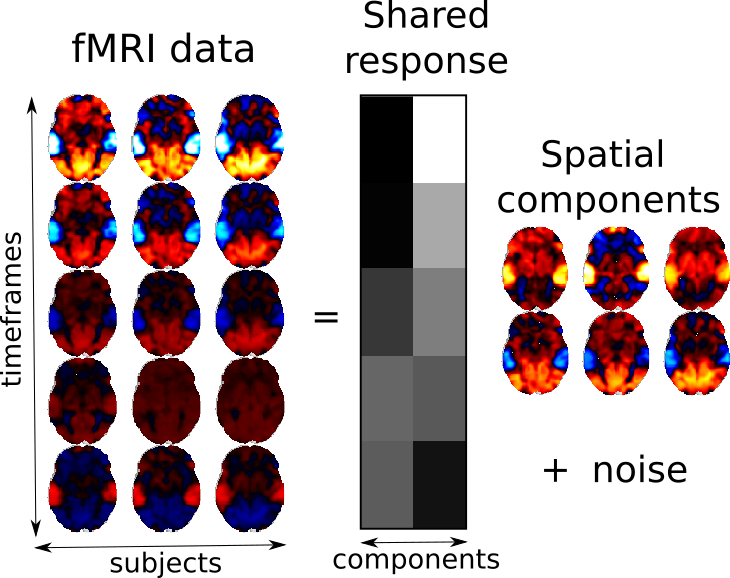
\includegraphics[scale=0.3]{figures/srm/conceptual_figure31.png}
  \caption{\textbf{Shared response model}: The raw fMRI data are modeled as a weighted combination of subject-specific spatial components with additive noise. The weights are shared between subjects and constitute the shared response to the stimuli.}
  \label{fig:srm:conceptual_figure}
\end{figure}

In~\cite{chen2015reduced, anderson2016enabling}, two versions of the shared response model are
introduced which we now present.
\subsubsection{Deterministic shared response model}
\label{sec:deterministicsrm}
The deterministic shared response model sees both the mixing matrices $A_i$ and
the shared response $\sbb$ as parameters to be
estimated. The noise variance is fixed to a multiple of identity: $\forall i,
\Sigma_i=\sigma^2 I_v$ where $\sigma$ is an hyper-parameter to choose.
The model is optimized by maximizing the log-likelihood.
The likelihood is given by: $p(\xb) = \prod_i \Ncal(\xb_i; A_i \sbb, \sigma^2 I)$ and
therefore the negative log-likelihood is given up to a constant independent of
$A_i$ and $\sbb$ by:
\begin{align}
  \loss = \sum_i \|A_i \sbb - \xb_i \|^2 = \| \sbb \|^2 -2 \langle A_i \sbb, \xb_i \rangle + \| \xb_i \|^2
  \label{eq:detsrmloss}
\end{align}
The negative log-likelihood $\loss$ is optimized by performing alternate minimization on $(A_1 \dots A_m)$
and $\sbb$. Note that the hyper-parameter $\sigma$ does not have an influence on
the loss and can therefore be safely ignored.

The gradient with respect to $\sbb$ is given by $ \sum_i A_i^{\top}(A_i \sbb -
\xb_i) = \sum_i (\sbb -
A_i^{\top} \xb_i)$
yielding the closed form updates:
\begin{equation}
  \sbb \leftarrow  \frac1m \sum_i (A_i^{\top} \xb_i)
  \label{eq:srm:supdate}
\end{equation}

From \eqref{eq:detsrmloss}, minimizing $\loss$ with respect to $A_i$ is
equivalent to maximizing $\langle A_i, \xb_i \sbb^{\top} \rangle$ and therefore we
have:
\begin{equation}
  A_i \leftarrow  \Pcal(\xb_i \sbb^T)
  \label{eq:detsrm:Aiupdate}
\end{equation}
where $\Pcal$ is the projection on the Stiefel manifold: $\Pcal(M) = M
(M^{\top}M)^{-\frac12}$.

The complexity of Deterministic SRM is in $\bigO(\mathrm{n_{iter}} mpvn)$ where
$n$ is the number of samples and $\mathrm{n_{iter}}$ the number of iterations.
We monitor the convergence by looking at the $\ell_{\infty}$ norm of the
gradient. We can monitor the gradient without any increase in complexity.
Indeed, after the updates with respect to each mixing matrix have been
carried out, only the gradient with respect to $\sbb$ remains: $\sum_i
(\sbb - A_i^{\top}\xb_i)$. The algorithm is stopped when the
gradient is below a chosen tolerance.

\subsubsection{Probabilistic SRM}
\label{sec:probabilisticsrm}
In Probabilistic SRM , $\Sigma_i=\sigma_i^2 I_v$ and the shared
components are assumed to be Gaussian $\sbb \sim \Ncal(0, \Sigma_s)$.
In~\cite{chen2015reduced}, $\Sigma_s$ is only assumed to be definite positive. However,
as will be seen in the FastSRM chapter, enforcing a diagonal $\Sigma_s$ ensures
identifiability (provided the diagonal values are different). So we assume for
now on, that $\Sigma_s$ is diagonal.

The model is optimized via the expectation maximization algorithm.
Denoting $\VV[\sbb | \xb] = (\sum_i \frac1{\sigma_i^2} I +
\Sigma_s^{-1})^{-1}$ and $\EE[\sbb | \xb] = \VV[\sbb | \xb] \sum_i \frac1{\sigma_i^2}
A_i^{\top}\xb_i$, we have
\begin{align}
  p(\xb, \sbb) &= \prod_i \frac{\exp(-\frac{\|\xb_i - A_i \sbb \|^2}{2 \sigma_i^2})}{(2 \pi \sigma_i^{2v})^{\frac12}} \frac{\exp(-\frac12 \langle \sbb , \Sigma_s^{-1} \sbb \rangle )}{(2 \pi | \Sigma_s|)^{\frac12}} \\
               &= c_1 \exp(-\frac12 \left( \sum_i \frac1{\sigma_i^2}\|\xb_i\|^2 - 2  \langle \sum_i \frac1{\sigma_i^2} A_i^{\top}\xb_i, \sbb \rangle \right. \\& \left.+ \sum_i \frac1{\sigma_i^2} \| \sbb \|^2 + \langle \sbb, \Sigma_s^{-1} \sbb \rangle  \right)) \\
               &= c_2 \exp(-\frac12 \left( \langle  \sbb - \EE[\sbb | \xb], \VV[\sbb | \xb]^{-1} ( \sbb - \EE[\sbb | \xb])  \rangle \right)) \label{probsrmcompleted}
\end{align}
where $c_1 = \frac1{(2 \pi \sigma_i^{2v})^{\frac12}}\frac1{(2 \pi |
  \Sigma_s|)^{\frac12}}$ and $c_2 = c_1 \exp(-\frac12( \sum_i
\frac1{\sigma_i^2}\|\xb_i\|^2 - \langle  \EE[\sbb | \xb], \VV[\sbb | \xb]^{-1} \EE[\sbb | \xb] \rangle))$ are independent of $\sbb$.
Therefore $\sbb| \xb \sim \Ncal(\EE[\sbb | \xb], \VV[\sbb, \xb])$

The negative completed log-likelihood is given by
\begin{align}
	\loss = \sum_i \frac12 v \log(\sigma_i^2) + \frac1{2 \sigma_i^2} \| \xb_i - A_i \sbb \|^2
\end{align}
updates are therefore given by:
\begin{align}
&\sigma_i^2 \leftarrow \frac1{v} (\| \xb_i - A_i \EE[\sbb|\xb]\|^2 + \| \diag(\VV[\sbb | \xb]) \|^2) \\
  &A_i \leftarrow \Pcal(\xb_i \EE[\sbb|\xb]^{\top}) \label{eq:psrm:Aiupdate} \\
  & \Sigma_s \leftarrow \VV[\sbb | \xb] + \EE[\sbb | \xb] \EE[\sbb | \xb]^{\top}
\end{align}

It is useful to access the log-likelihood to check the implementation of the
algorithm and monitor the convergence. From equation~\eqref{probsrmcompleted},
the likelihood is given by:
\begin{align}
  p(\xb) &= c_2 \int_{\sbb} \exp(-\frac12 \left( \langle  \sbb - \EE[\sbb | \xb], \VV[\sbb | \xb]^{-1} ( \sbb - \EE[\sbb | \xb])  \rangle \right)) d\sbb \\
         &= c_2 (2 \pi |\VV[\sbb | \xb]|)^{\frac12}
\end{align}
and so up to constants the negative log-likelihood is given by:
\begin{align}
  -\log(p(\xb)) = &\sum_i \frac{v}{2} \log(\sigma_i^2) + \frac12 \log(|\Sigma_s|) - \frac12 \log(|\VV[\sbb | \xb]|) \\ &+ \sum_i
  \frac12 \frac1{\sigma_i^2}\|\xb_i\|^2 - \frac12 \langle  \EE[\sbb | \xb], \VV[\sbb | \xb]^{-1} \EE[\sbb | \xb] \rangle
\end{align}
\textbf{XXX I am confused: why not simply the log of the above expression ?}

The complexity of Probabilistic SRM is $\bigO(\mathrm{n_{iter}} mpvn)$, the same as in
Deterministic SRM.
We can monitor the convergence by looking at the log-likelihood decrease at each iteration
and stop the algorithm when the magnitude of the decrease is below some
tolerance.
The storage requirements of Deterministic or Probabilistic SRM are in
$\bigO(mvn)$ which simply means that the dataset needs to hold in memory.

% \section{Related Work}
% \label{sec:rel_work}
% %

% %
% %

% %
% %
% %

% \textbf{Structured mixing matrices} One strength of our model is that we only assume that the mixing matrices are invertible and still enjoy identifiability whereas some other approaches impose additional constraints. For instance tensorial methods~\cite{beckmann2005tensorial} assume that the mixing matrices are the same up to diagonal scaling.
% %
% Other methods impose a common mixing matrix~\cite{cong2013validating, grin2010independent, calhoun2001fmri, Monti18UAI}. Like PCA, the Shared Response Model~\cite{chen2015reduced} (SRM) assumes orthogonality of the mixing matrices. While the model defines a simple likelihood and provides an efficient way to reduce dimension, the SRM model is not identifiable as shown in appendix~\ref{sec:app_identifiability}, and the orthogonal constraint may not be plausible.
% %

% \textbf{Matching components a posteriori} A different path to multi-subject ICA is to extract independent components with individual ICA in each subject and align them. We propose a simple baseline approach to do so called \emph{PermICA}.
% Inspired by the heuristic of the hyperalignment method~\cite{haxby2011common} we choose a reference subject and first match the components of all other subjects to the components of the reference subject. The process is then repeated multiple times, using the average of previously aligned components as a reference. Finally, group components are given by the average of all aligned components. We use the Hungarian algorithm to align pairs of mixing matrices~\cite{tichavsky2004optimal}.
% %
% Alternative approaches involving clustering have also been developed~\cite{esposito2005independent,bigdely2013measure}.

% \textbf{Deep Learning} Deep Learning methods, such as convolutional auto-encoders (CAE), can also be used to find the subject specific unmixing~\cite{chen2016convolutional}. While these nonlinear extensions of the aforementioned methods are interesting, these models are hard to train and interpret. In the experiments on fMRI data in appendix~\ref{appendix_reproduce}, we obtain better accuracy with MultiView ICA than that of CAE reported in~\cite{chen2016convolutional}.

% \textbf{Correlated component analysis} Other methods can be used to recover the shared neural responses such as the correlated component approach of Dmochowski~\cite{dmochowski2012correlated}. We benchmark our method against its probabilistic version~\cite{kamronn2015multiview} called BCorrCA in Figure~\ref{fig:meg}. Our method yields much better results. 

% \textbf{Autocorrelation} Another way to perform ICA is to leverage spectral diversity of the components rather than non-Gaussianity.
% %
% These methods are popular alternative to non-Gaussian ICA in the single-subject setting~\cite{tong1991indeterminacy, belouchrani1997blind, pham1997blind} and they output significantly different components than non-Gaussian ICA~\cite{delorme2012independent}.
% %
% Extensions to multiview problems have been proposed~\cite{lukic2002ica, congedo2010group}.

\part{FastSRM: An efficient implementation of the shared response model}
\label{part:fastsrm}
\chapter{FastSRM theory}
\label{ch:fastsrm1}
In the previous chapter, we have decribed multiple unsupervised methods to analyze
multiview data.
As described in section~\ref{sec:srm:review}, the shared response
model~\cite{chen2015reduced} (SRM) is a multi-view latent factor model. It sees
the data $(\xb_i)_{i=1}^m$ as:
\begin{align}
  &\xb_i = A_i \sbb + \nb_i \\
  &A_i^{\top}A_i = I_p
\end{align}
with $\nb_i \sim \Ncal(0, \Sigma_i)$ where $\Sigma_i = \sigma^2 I_v$ in
deterministic SRM and $\Sigma_i = \sigma_i^2 I_v$ in probabilistic SRM.

When working with high dimensional data, SRM is particularly
interesting as it provides a principled way to perform dimension reduction. Note that this
contrasts with ICA-like methods that do not incorporate dimension reduction in their model.

However SRM has initially been designed to work within regions of interest using
only few subjects. When using full brain data, computational costs become
high. In addition, memory requirements are difficult to meet since the full dataset needs to hold
in memory.

Fortunately, these high costs can be reduced. Intuitively, since the shared
response lives in a reduced space, a compressed representation of the input is
good enough to find a suitable estimate of the shared response.
FastSRM implements this idea. It turns out that there exists an optimal
compression of the input for which we can obtain the same solution as
with the full data.

\section{The FastSRM algorithm}
SRM algorithms use different set of parameters $\theta$ to represent the data.
In deterministic SRM $\theta = (A_i)_{i=1}^m, \sbb$ where $(A_i)_{i=1}^m$ are the
mixing matrices and $\sbb$ the shared response while in probabilistic SRM $\theta
= (A_i)_{i=1}^m, \Sigma_s, (\sigma_i)_{i=1}^m$ where $(A_i)_{i=1}^m$ are the
mixing matrices, $(\sigma_i)_{i=1}^m$ the noise levels and $\Sigma_s$ the
components variance.

In fMRI, the classical approach used to reduce the data is to apply an atlas.
A deterministic atlas such as~\cite{bellec2010multi} is a parcellation of the
brain into $r$ regions. Reducing an image using a deterministic atlas corresponds to
averaging the signal within each region of the atlas. A probabilistic atlases such
as~\cite{dadi_fine-grain_2020} describes each region as a set of weights across
the full brain. Therefore, the image reduction can be done with a matrix product.

In FastSRM we consider a set of view specific atlases $U_i \in \RR^{v \times r}$ such that
$U_i^{\top}U_i = I_r$ where $r$ is the number of regions in the atlas.
Data are reduced using $\zb_i = U_i^{\top} \xb_i$ and an SRM algorithm is applied
on data $\zb_i$ yielding parameters $\theta'$.
The figure~\ref{fig:srm:conceptual} illustrates this process.

Note that the parameters obtained with FastSRM $\theta'$ are different
from the parameters obtained with the corresponding SRM algorithm $\theta$ (the unmixing matrices in $\theta'$ do not even have the same shape as the unmixing matrices in $\theta$).
However, as we will see in the next section, there exists an explicit and exact
correspondence between $\theta$ and $\theta'$ although in the case of
probabilistic SRM, the algorithm applied on reduced data needs to be slightly modified in order to
obtain these guarantees. 

\begin{figure}
  \centering
  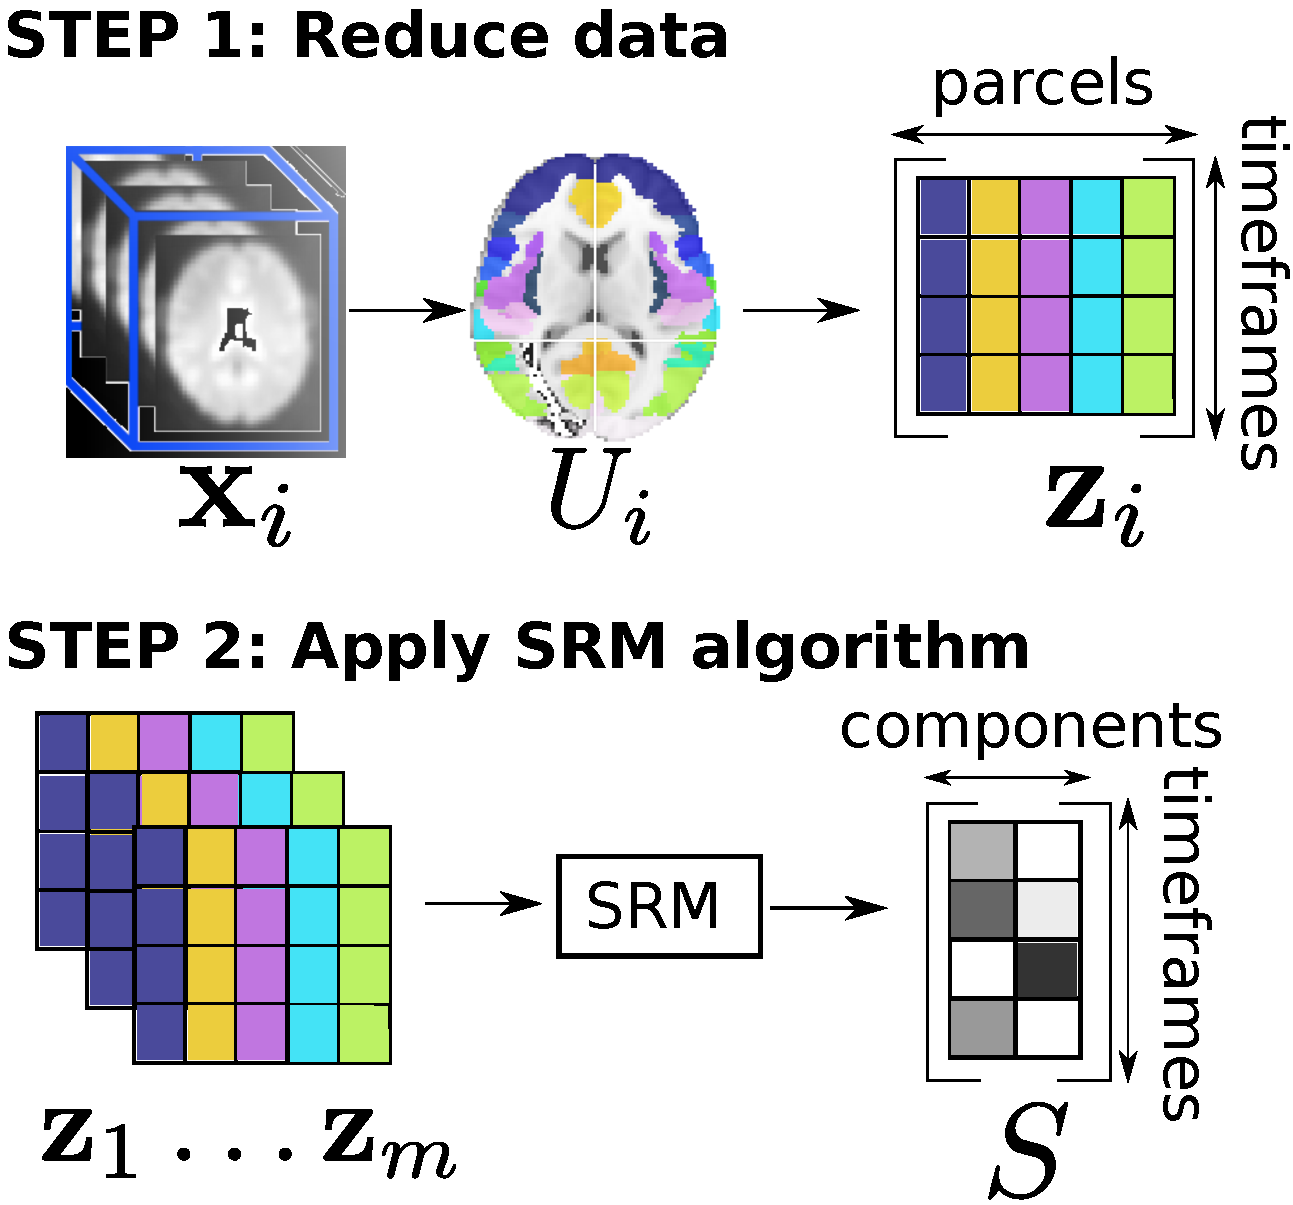
\includegraphics[scale=0.34]{figures/srm/conceptual_figure2.pdf}
  \caption{\textbf{FastSRM algorithm} In step 1, data $\xb_i$ are projected onto an
    atlas $U_i$ that may depend on the subject $i$ (top). In step 2 a SRM algorithm is applied on reduced data to compute the shared response.}
  \label{fig:srm:conceptual}
\end{figure}

From a computational stand point, the dimension reduction provides
a large reduction in memory usage. Indeed as the original data are seen only
once, it is no longer necessary to keep the full dataset in memory (we can load
data $\xb_i$ one after the other and similarly for the atlases $U_i$). Therefore
the memory consumption is only in $\bigO(vn)$ (where $v$ is the number of voxels
and $n$ is the number of samples) which is lower than SRM by a factor of $m$,
the number of subjects. The number of subjects is typically between $10$ and
$1000$. This yields a practical benefit: on fMRI datasets with many subjects, one no longer needs a large cluster to run the shared response model but only a modern laptop.
Additionally, low memory consumption reduces the
risk of thrashing~\cite{denning1968thrashing}, a phenomenon that causes large
increase in computation time when the memory used is close to the total available
memory in the hardware.

After preprocessing, the reduced representation $\zb_i$ is used instead of the
original data $\xb_i$ yielding a time complexity of $\bigO(
\mathrm{T_{preprocessing}} + \mathrm{n_{iter}} mpnr)$.
Let us highlight that in practice, it often happens that an experiment is run
multiple times such as when cross validated results are needed. In these cases,
the pre-processing is performed only once and the apparent complexity becomes
$\bigO(\mathrm{n_{iter}} mpnr)$ which is faster than SRM by
a factor of $\frac{v}{r}$. The number of regions in large atlases is about $r=1000$ and in full brain data, the number of voxels is about $300~000$ so that $\frac{v}{r}$ is typically about $1000$.

It remains to show how to draw a correspondence between FastSRM and SRM which is addressed in the following section.

\section{Optimal atlases}
In principle, FastSRM can be used with any atlas. 
However, in general, working with reduced data induces a loss of information and
therefore there is little hope to recover the parameters that would have been obtained from SRM from the parameters of FastSRM.
However, in this section, we show that there exists an optimal atlas in the sense that SRM and FastSRM yield the same results.

Let us consider $\xb_i = U_{\xb_i} \zb_i$ a PCA of $\xb_i$. As the number of
samples $n$ is lower than the number of features $U_{\xb_i} \in \RR^{v \times n}$ and $\zb_i \in \RR^{n}$.  We also have $U_{\xb_i}^{\top}U_{\xb_i} = I$.
Therefore $U_{\xb_i}$ constitutes a possible choice of subject specific atlas.

As the next property shows, $U_{\xb_i}$ constitutes an optimal atlas for deterministic FastSRM.
\begin{prop}[Optimal atlas for deterministic FastSRM]
  Let $(A_i)_i, \sbb$ be the solution obtained by deterministic SRM on data
  $\xb_i$ and $(A_i')_i, \sbb'$ the solution obtained by deterministic FastSRM on
  data $\xb_i$ using atlas $U_{\xb_i}$ where $\xb_i = U_{\xb_i} \zb_i$ is a PCA
  of $\xb_i$. Then $A_i = U_{\xb_i}A_i'$ and $\sbb = \sbb'$. 
\label{prop:optimaldetsrm}
\end{prop}
\begin{proof}
Updates of the mixing matrices $A_i$ in deterministic SRM
equation~\eqref{eq:detsrm:Aiupdate} can be written:
\begin{align}
  A_i &\leftarrow \Pcal(\xb_i \sbb^T)= U_{\xb_i}\Pcal(\zb_i \sbb^T)
  \label{eq:fastdetsrm:Aiupdate}
\end{align}
where $\Pcal$ is the projection on the Stiefel manifold: $\Pcal(M) = M
(M^{\top}M)^{-\frac12}$.


Therefore we can look for $A_i$ as $A_i = U_{\xb_i} \tilde{A_i}$. $\tilde{A_i}$ is
orthogonal. Indeed
\begin{align}
  &A_i^{\top} A_i = I_p \\
  & \implies \tilde{A_i}^{\top}U_{\xb_i}^{\top} U_{\xb_i} \tilde{A_i} = I_p \\
  & \implies \tilde{A_i}^{\top} \tilde{A_i} = I_p
\end{align}

Then, we use the fact that
\begin{align}
  \|\xb_i - A_i \sbb \|^2 = \| U_{\xb_i}\zb_i - U_{\xb_i}\tilde{A_i} \sbb\|^2 = \| \zb_i - \tilde{A_i} \sbb \|^2
  \label{eq:equality:xy}
\end{align}
Therefore, the solution of deterministic SRM on data $(\zb_i)_{i=1}^m$ and
$(\xb_i)_{i=1}^m$ are linked by the change of parameters $A_i = U_{\xb_i}A_i'$ and
$\sbb = \sbb'$ where $A_i' = \tilde{A_i}$. This concludes the proof.
\end{proof}

In the case of probabilistic SRM we can obtain very similar results. However the
algorithm applied on reduced data need to be slightly modified.
We call probSRM($\psi$) the probabilistic SRM algorithm modified such that
updates
\begin{align}
\sigma_i^2 \leftarrow \frac1{v} (\| \xb_i - A_i \EE[\sbb|\xb]\|^2 + \| \diag(\VV[\sbb | \xb]) \|^2)
\end{align}
are replaced by updates
\begin{align}
  \sigma_i^2 \leftarrow \frac1{\psi} (\| \xb_i - A_i \EE[\sbb|\xb]\|^2 + \| \diag(\VV[\sbb | \xb]) \|^2)
\end{align}

We have the following result:
\begin{prop}[Optimal atlas for probabilistic FastSRM]
  Let $(A_i)_i, \sigma_i, \Sigma_s$ be the solution obtained by probabilistic SRM on data
  $\xb_i$ and $(A_i')_i, \sigma_i', \Sigma_s'$ the solution obtained by ProbSRM($v$) on
  data $\zb_i = U_{\xb_i}^{\top} \xb_i$.Then $A_i = U_{\xb_i}A_i'$, $\sigma_i =
  \sigma_i'$ and $\Sigma_s = \Sigma_s'$. 
  \label{prop:optimalprobsrm}
\end{prop}
\begin{proof}
  Updates of the mixing matrices $A_i$ in probabilistic SRM equation~\eqref{eq:psrm:Aiupdate}. We get:
  \begin{align}
    A_i &\leftarrow U_{\xb_i}\Pcal(\zb_i \EE[\sbb| \xb_i]^T)
    \label{eq:fastprobsrm:Aiupdate}
  \end{align}
  so we can look for $A_i$ as $A_i = U_{\xb_i} \tilde{A_i}$ and, as in the
  deterministic case, $\tilde{A_i}$ is orthogonal.
  Therefore equality~\eqref{eq:equality:xy} holds.
  
  Then we consider the negative log-likelihood of probabilistic srm:
  \begin{align}
    \loss &= \sum_i \frac12 v\log(\sigma_i^2) + \frac12 \log(|\Sigma_s|) + \int_{\sbb} \sum_i \frac1{2 \sigma_i^{2}}\|\xb_i - A_i \sbb \|^2 \\& \enspace + \frac12 \dotp{ \sbb }{ \Sigma_s^{-1} \sbb }  d\sbb \\
          &= \sum_i \frac12 v \log(\sigma_i^2) + \frac12 \log(|\Sigma_s|) + \int_{\sbb} \sum_i \frac1{2 \sigma_i^{2}}\|\zb_i - \tilde{A_i} \sbb \|^2 \\& \enspace+ \frac12 \dotp{ \sbb }{ \Sigma_s^{-1} \sbb }  d\sbb
  \end{align}
  where we use equality~\eqref{eq:equality:xy}.
  Optimizing the log-likelihood via expectation maximization yields the exact
  same updates as probabilistic srm on data $\zb_i$
  except that updates
  \begin{align}
    \sigma_i^2 \leftarrow \frac1{t} (\| \zb_i - \tilde{A_i} \EE[\sbb|\zb]\|^2 + \| \diag(\VV[\sbb | \zb]) \|^2)
  \end{align}
  are replaced by updates
  \begin{align}
    \sigma_i^2 \leftarrow \frac1{v} (\| \zb_i - \tilde{A_i} \EE[\sbb|\zb]\|^2 + \| \diag(\VV[\sbb | \zb]) \|^2)
  \end{align}

  The updates in both algorithms are linked  by $A_i = U_{\xb_i}A_i'$ where
  $A_i' = \tilde{A_i}$, $\sigma_i' =
  \sigma_i$ and $\Sigma_s'  = \Sigma_s$.

  This concludes the proof.
\end{proof}

The properties~\ref{prop:optimaldetsrm} and~\ref{prop:optimalprobsrm} show that
no information is lost by replacing $\xb_i \in \RR^v$ by its reduced representation $\zb_i \in \RR^n$.
A key property of the optimal atlas $U_{\xb_i}$ is that it is valid whether or
not the model for deterministic (respectively probabilistic) SRM holds.

A complexity analysis shows that finding the optimal atlas becomes the limiting
step of the pipeline. Even with fast implementations, the subject specific PCA
is costly. However FastSRM only works on $\zb_i$ so we do not need to know the value of $U_{\xb_i}$ straight away.
In practice, we observe data $X_i \in \RR^{v \times n}$ and we want to get $Z_i
\in \RR^{n \times n}$ such that $X_i = U_{\xb_i} Z_i$. This can be done by performing an
SVD of $X_i^{\top} X_i$ yielding $X_i^{\top}X_i= V_i D_i V_i^{\top}$ and setting $Z_i = D_i^{\frac12} V_i^{\top}$.
Although the product $X_i^{\top} X_i$ has complexity $\bigO(vt^2)$ there is
exactly $vt^2$ multiplications and additions so it costs a lot less than the PCA
on full data. When estimates of the mixing matrices are needed, they can be obtained by
applying equation~\eqref{eq:fastdetsrm:Aiupdate} in the deterministic SRM case and
equation~\eqref{eq:fastprobsrm:Aiupdate} in the probabilistic SRM case which only costs
$\bigO(mvp^2)$.
In practice the cost of the matrix products $X_i^{\top} X_i$ is often still the
limiting step of the pipeline (this depends on the number of iterations) but as
we show in the next chapter, this yields to great speed up compared to classical
SRM implementations. Note than if memory allows it, these matrix products can easily be done using multiple cores in parallel.

% In the next section, we investigate approaches to reduce the preprocessing time.

% \section{Efficient approximation of optimal atlases}
% As we have seen in the previous section, if $U_i = U_{\xb_i}$ where $\xb_i =
% U_{\xb_i} \zb_i$ is a PCA of $\xb_i$, then $U_i$ is an optimal atlas.
% A natural follow-up is to look for atlases that are close to optimal in the
% sense that the inertia $\| (I - U_i U_i^{\top}) \xb_i \|$ is low but are fast to
% compute and such that projecting data on the atlas is a cheap operation.

% Deterministic atlases are interesting as they allow for fast data projection
% (computing $U_i \xb_i$ only costs $\bigO(v)$). Furthermore, they are thought to
% be well-suited to fMRI data as they reduce noise via smoothing (this argument is
% detailed in~\cite{hoyos2018recursive}).
% %
% A first approach is to use existing deterministic atlases for fMRI data such as 
% ~\cite{schaefer2017local} or~\cite{bellec2010multi}. As theses atlases
% attempt to reduce the dimension of fMRI signals without losing too much signal,
% there is hope for the inertia to be small.
% RENA, the clustering approach
% of~\cite{hoyos2018recursive}, is also appealing as it is optimized to give low
% inertia while the cost of finding the deterministic atlas is low (computing $U_i$ only costs
% $\bigO(vn)$). As the number $r$ of regions increases, the inertia decreases
% and the approximation becomes better and better. An other possibility is to
% perform a PCA with a number of components $r < n$.

% The approaches previously described attempt to approximate $U_i$ by a
% deterministic atlas. Another possibility is to approximate directly $\zb_i$ via
% random projection.
% Let us call $X_i \in \RR^{v,
%   n}$ our data matrix. Following~\cite{mahoney2016lecture} (section 14.4), we
% can approximate $X_i^{\top} X_i$ by $\tilde{C} = \sum_{j \in \mathcal{J}} \frac1{p_j r} \xb_{ij}^{\top} \xb_{ij}$ where $\xb_{ij}$ is the $j$-th line of
%   $X_i$ and $\mathcal{J}$ is a set of $r$ indexes such that $\mathcal{J}$ contains
%   index $j$ with probability $p_j$. The most simple choice is $p_j=\frac1{v}$
%   which we use in our implementations. Other choices are possible, we refer the reader to section 15
%   of~\cite{mahoney2016lecture} for more details.  Computing an approximation of $X_i^{\top} X_i$ is interesting
%   because the SVD of $X_i^{\top} X_i$ allows us to recover the reduced data
%   $Z_i$ up to an irrelevant sign indeterminacy. 
%   If spatial maps $A_i$ are needed, they can be recovered from the data using the formula
%   $A_i \leftarrow \mathcal{P}(\xb_i \sbb^{\top})$ (in the deterministic SRM case) or
%   $A_i \leftarrow \mathcal{P}(\xb_i \EE[\sbb^{\top}|\xb])$ (in the probabilistic SRM case).

  Up to now, we have assumed that the covariance of components is diagonal in
  probabilistic SRM. In the next section we justify this assumption.

\section{Identifiablity of the shared response model}
We first show why deterministic SRM and probabilistic SRM without any
restriction on the covariance of the components can
only recover unmixing matrices up to an arbitrary rotation.

Let us consider data $\xb_i$ generated from deterministic SRM (meaning
deterministic SRM holds exactly for these data) with
mixing matrices $A_i$, shared response $\sbb$ and noise covariance $\sigma$.
Then deterministic SRM, with parameters $A'_i = A_i R$ and $\sbb' = R^{\top} \sbb$ where
$R \in \RR^{k \times k}$ is an orthogonal matrix, also
generates $\xb_i$.
This shows that deterministic SRM is not identifiable.

Similarly, in the probabilistic SRM case, if data $\xb_i$ are generated from the
probabilistic SRM model with 
parameters $A_i$, $\Sigma_s$, $\sigma_i^2$ (where $\Sigma_s$ can be any
symmetric positive definite
matrix) then the probabilistic SRM model with parameters $A_iR$, $R^{\top} \Sigma_s R$, $\sigma_i^2$  where
$R \in \RR^{k \times k}$ is an orthogonal matrix also generate $\xb_i$.
This shows that if no constrains are imposed on $\Sigma_s$,
then probabilistic SRM is not identifiable.


Then, we show that if $\Sigma_s$ is assumed to be diagonal, then probabilistic
SRM is identifiable under weak assumptions :
\begin{prop}[Identifiability of probabilistic SRM]
  \label{prop:fastsrm:identifiability}
  Let $\xb_i$ be generated from a probabilistic SRM with parameters 
  $A_i$, $\Sigma_s$, $\sigma_i^2$ (where $\Sigma_s$ is diagonal positive with
  distinct values on the diagonal) and assume there exists another set of parameters $A_i'$, $\Sigma_s'$,
  ${\sigma_i'}^2$ (where $\Sigma_s'$ is diagonal positive with
  distinct values on the diagonal) that also generate $\xb_i$.
Then if $m\geq 3$, $A_i' = A_i P^{\top}$, $\Sigma_s'= P\Sigma_sP^{\top}$ and
  ${\sigma_i^2}' = {\sigma_i}^2$ where $P$ is a sign and permutation matrix
  (meaning $P$ is the product of a diagonal matrix with values in $\{-1, 1\}$
  and a permutation matrix).
\end{prop}
\begin{proof}
  Let us consider $\EE[\xb_i \xb_j^{\top}]$ for $i \neq j$.
  We have:
  \begin{equation}
  A_i \Sigma_s A_j^{\top} = A_i' \Sigma_s' {A_j'}^{\top}
  \label{eq:fastsrm:svd}
  \end{equation}
  up to re-ordering, equation~\eqref{eq:fastsrm:svd} gives two singular value
  decompositions of the same matrix.
  Therefore, by unicity of the singular value decomposition we have:
  $\Sigma'_s = P_i \Sigma_s P_j^{\top}$ and $A_i' = A_i P_i^{\top}$ and $A_j =
  A_j P_j^{\top}$ where $P_i$ and $P_j$ are sign and permutation matrices.
  Since there are more than three subjects, there exists subject $z$ such that
  $\Sigma'_s = P_i \Sigma_s P_z^{\top}$ and therefore
  $P_i \Sigma_s P_z^{\top} =  P_i \Sigma_s P_j^{\top}$ so that $P_j =
  P_z$. So all sign and permutations are the same and we call $P$ their
  common value.
  Then we consider
  $\EE[\xb_i \xb_j^{\top}] = A_i \Sigma A_i^{\top} + \sigma^2 I_v = A_i' \Sigma_s'
  {A_i'}^{\top} + {\sigma^2}' I_v$
  so we get ${\sigma^2}' = {\sigma^2}$
\end{proof}

Proposition~\eqref{prop:fastsrm:identifiability} justifies that
$\Sigma_s$ should be assumed to be diagonal in probabilistic SRM.
In addition, working with a diagonal covariance matrix allows to speed up
slightly the computations (although this does not change the time complexity of
the algorithm).

In the next chapter, we investigate how FastSRM works in practice compared to
available implementations.

\chapter{FastSRM experiments}
\label{ch:fastsrm2}
\section{Experiments}
\subsection{Comparing Fitting time and performance of FastSRM and
  SRM on synthetic data}
We generate data $\xb_i$ according to the model of Probabilistic SRM. We sample the value of the subject specific noise level from a normal
distribution: $\sigma_i \sim \Ncal(0, 0.1)$. The mixing matrices $A_i$
are obtained by sampling their coefficient from a standardized normal distribution.
Lastly, the covariance of the shared response $\Sigma_s$ is diagonal and the
diagonal values are obtained by sampling from a Dirichlet distribution with
parameter $(1 \dots 1)$.
The number of voxels is fixed to $v=125~000$. The number of samples is given by
$n=1000$. We use $m=10$ subjects and $p=50$ components.

We benchmark different implementations of deterministic SRM and probabilistic
SRM in terms of fitting time and performance. The basic SRM described in
section~\ref{sec:probabilisticsrm} and~\ref{sec:deterministicsrm} is refered to
as \emph{NONE} because no atlas is used. 
\emph{OPTIMAL} is the FastSRM algorithm with optimal atlas which is provably
equivalent to using no atlas. \emph{ReNA} uses the fast clustering approach
of~\cite{hoyos2018recursive} with a number of regions is equal to the number of
components: $r=n$. \emph{PROJ} is the random projection approach that
approximates the optimal reduced data using only $r=5n$ voxels. Lastly
\emph{PCA} applies SRM algorithms to data reduced with a PCA using $r=p+1$ components \textbf{XXX Why  + 1 ?}.

For any number of iterations between 1 and 100.
We measure the performance of an algorithm by computing the error between the true component $S \in \RR^{p, n}$ and
the predicted component $\hat{S} \in \RR^{p, n}$ using the quantity:
$\mathrm{mse}(\hat{S}, S) = min_{A \in \RR^{p, p}} \|A \hat{S} - S \|^2_F =  \|S
\hat{S}^{\dagger}\hat{S} - S \|^2_F$. This way of measuring errors is
insensitive to the indeterminacies in DetSRM.
We measure the fitting time in seconds.
Lastly, we measure convergence by computing the gradient $\el_{\infty}$ norm in
case of DetSRM given by $\max(\abs{G})$ where $G$ is the gradient. For ProbSRM
algorithms the convergence is given by the distance between consecutive values of the loss.

Results are plotted in figure~\ref{fig:srm:synthetic_gradient}. 
We empirically see that the optimal approach is equivalent to using no atlas in
terms of performance. Among approximate methods, the projection
method yields the best results but are quite far away from optimal results.
In general probabilistic methods gives a much better fit than their deterministic
counterpart which shows the superiority of likelihood based methods.
In terms of fitting time, we see that atlas based methods spend most of the time
computing the reduced representation but their total fitting time depends only
weakly on the number of iterations performed. When no atlas is used, the number
of iterations has a very strong impact on performance. The approximate methods
\emph{RENA} and \emph{PROJ} are much faster than other methods but
the \emph{PROJ} one yields much better results. The \emph{PCA} method is
almost as slow as the \emph{OPTIMAL} one while giving much worse results.
Comparing the use of an \emph{OPTIMAL} atlas to using \emph{NONE}, we see that
using the optimal atlas is faster as long as the number of iterations is greater
than $30$.
Looking at the convergence curves, we see that even after $100$ iterations, algorithms did
not fully converge. This means that in practice a much larger number of
iterations is needed which justifies why the \emph{OPTIMAL} atlas method is better.
Lastly, when the time budget is very tight, using an approximate atlas with the
\emph{PROJ} method is a better choice than
using SRM with less iterations. 

\begin{figure}
  \centering
  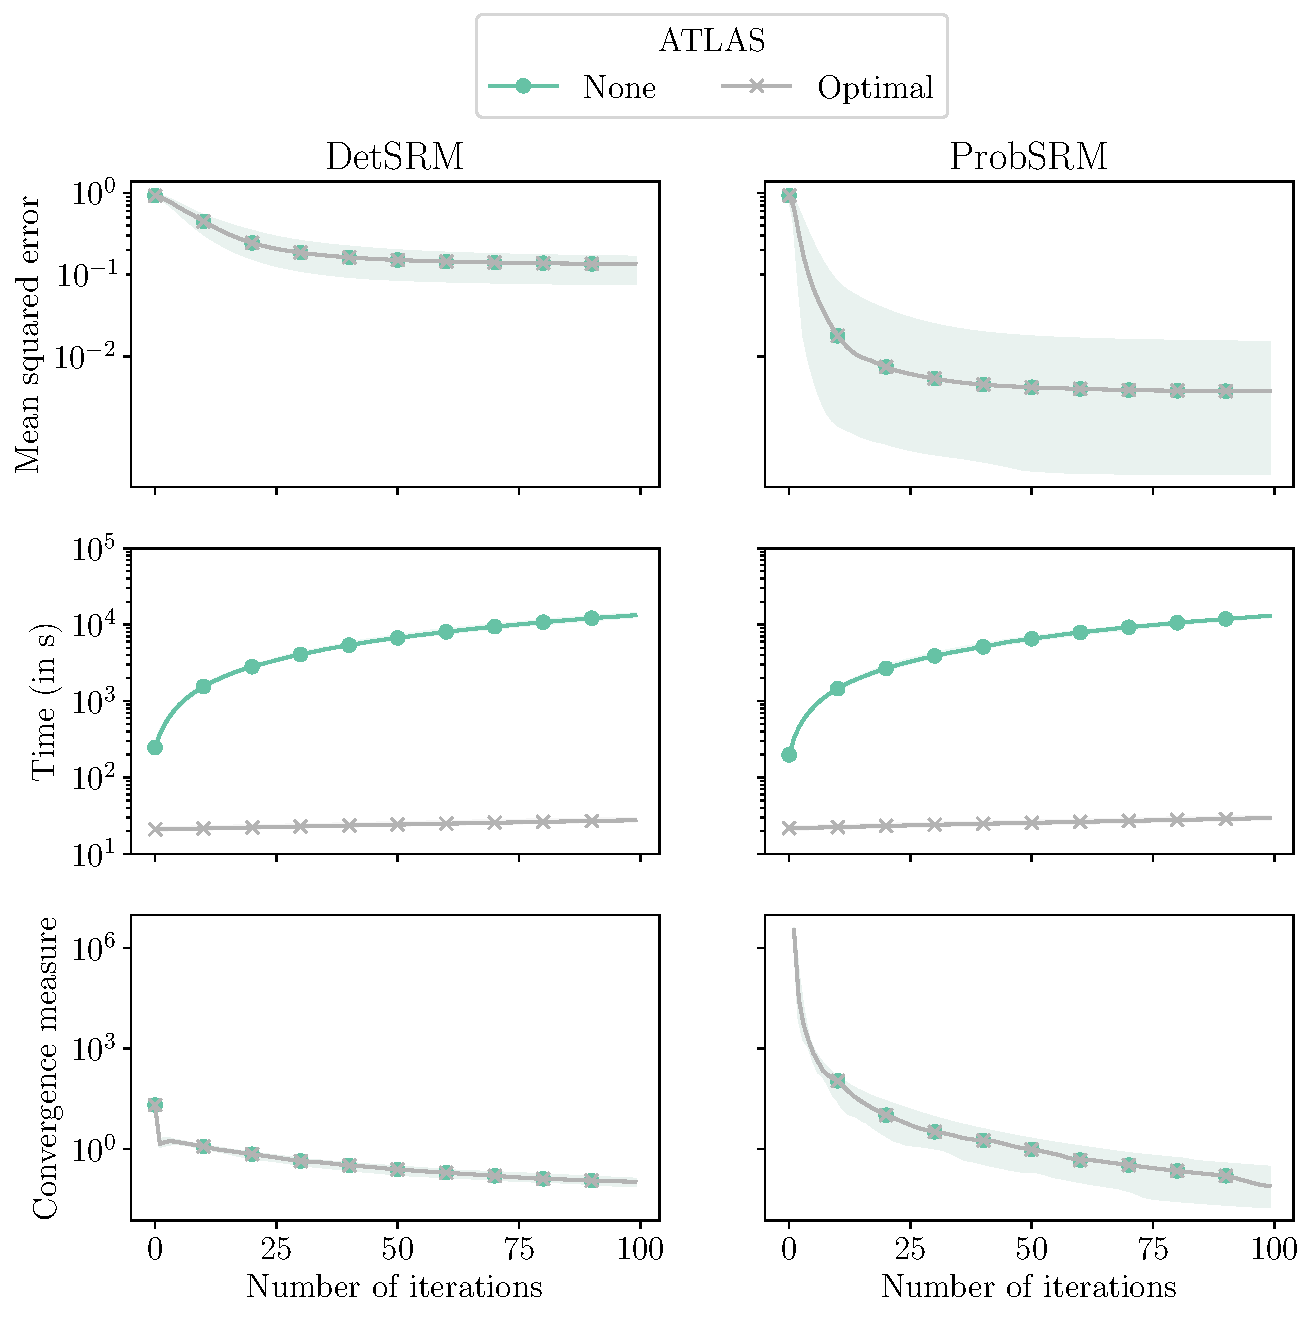
\includegraphics[width=\textwidth]{figures/srm/synthetic_gradient.pdf}
  \caption{\textbf{Benchmark of SRM algorithms on synthetic data: } Performance,
    fitting time and convergence of SRM algorithms (left) Deterministic SRM
    (right) Probabilistic SRM. \textbf{XXX Develop a little bit}}
  \label{fig:srm:synthetic_gradient}
\end{figure}





\textbf{fMRI data and preprocessing} 
We evaluate the performance of our approach on four different fMRI datasets.
%
\textbf{XXX It would be mroe logical to present the datasets before.}
The \emph{sherlock} dataset~\cite{chen2017shared} contains recordings of 16 subjects watching an episode of the BBC TV show "Sherlock" (50 mins).
%
The \emph{forrest} dataset~\cite{hanke2014high} was collected while 19 subjects were listening to an auditory version of the film "Forrest Gump" (110 mins).
%
The \emph{clips} dataset~\cite{ibc} was collected while 12 participants were exposed to short video clips (130 mins).
%
The \emph{raiders} dataset~\cite{ibc} was collected while 11 participants were watching the movie "Raiders of the Lost Ark" (110 mins).
%
The \emph{raiders-full} dataset~\cite{ibc} is an extension of the \emph{raiders} dataset where the first two scenes of the movie are shown twice (130 mins).
%
Like \cite{zhang2016searchlight}, we used full brain data. The rest of the preprocessing is identical to \cite{chen2017shared}. See \ref{preprocessing} for a detailed description of the datasets and preprocessing steps. Unless stated otherwise we use spatially unsmoothed data, except for the \emph{sherlock} dataset, for which the available data are already preprocessed with a 6\,mm spatial smoothing. All datasets are built from successive acquisitions called \emph{runs} that typically last 10 minutes each.
%

\textbf{Between subjects time-segment matching} \textbf{XXX}
\label{timesegment_expe}
%
\textbf{XXX Deserved more explanations: whay is it used ? Bhy is it a good metric ?}
We reproduce the time-segment matching experiment in
\cite{chen2015reduced}. 
We split the runs into a train and test set. After fitting the model on the training set, we apply the forward operator \textbf{XXX Undefined so far} of each subject on the test set yielding individual components matrices. We estimate the shared responses by averaging the individual components of each subjects but one.  We select a target time-segment (9 consecutive timeframes) in the shared responses and try to localize the corresponding time segment in the components of the left-out subject using a maximum-correlation classifier.
This is a standard evaluation of SRM-like methods also used in  \cite{chen2015reduced}, \cite{guntupalli2018computational}, \cite{Nastase741975} or
\cite{zhang2016searchlight}.
%
The time-segment is said to be
correctly classified if the correlation between the sample and target
time-segment is higher than with any other time-segment (partially overlapping time windows are excluded).
%
We use 5-Fold cross-validation across runs: the training set contains 80\% of the runs and the test set 20\%, and repeat the experiment using all possible choices for left-out subjects. 
%
The mean accuracy is reported in Figure~\ref{fig:timesegment} (bottom). 
%

We would like to highlight here that these experiments are not exactly the same as in~\cite{chen2015reduced} as we use full brain data and they use regions of interest. The code used for this experiment is very similar to the tutorial in \url{https://brainiak.org/tutorials/11-SRM/}. We use the SRM implementation in Brainiak~\cite{kumar2020brainiak}. Also note that the Raiders dataset is different from the one used in~\cite{chen2015reduced}, as it involves different subjects, and because data were acquired in a different neuro-imaging center.

\textbf{Reconstructing the BOLD signal of missing subjects}
\label{sec:srm:reconstruction}

We want to show that once unmixing matrices have been learned, they can be
used to predict
evoked responses across subjects, which can be useful to perform transfer learning~\cite{zhang2018transfer}. \textbf{XXX I don't see the point}
%
We split the data into three groups. First, we randomly choose $80\%$ of all runs from all subjects to form the training set.
%
Then, we randomly choose $80\%$ of subjects and take the remaining $20\%$  runs as testing set.
%
The left-out runs  of the remaining $20\%$ subjects form the validation set.
%
The compared algorithms are run on the training set and evaluated using the testing and validation sets.
%
After an algorithm is run on training data, it defines for each subject a \emph{forward operator} that maps individual data to the component space and a \emph{backward operator} that maps the component space to individual data. For instance in ICA \textbf{XXXWhy are wa talking about ICA ?} the forward operator is the product of the dimensionality reduction projection and unmixing matrix.
%
We estimate the shared responses on the testing set by applying the forward operators on the testing data and averaging. Finally, we reconstruct the individual data from subjects in the validation set by applying the backward operators to the shared responses. We measure the difference between the true signal and the reconstructed one using voxel-wise $R^2$ score. The $R^2$ score between two series $\xb \in \bbR^n$ and $\yb \in \bbR^n$ is defined as
$R^2(\xb, \yb) = 1 - \frac1{n\Var(\yb)}\sum_{t=1}^n (x_t - y_t)^2$, where $\Var(\yb) = \frac1n\sum_{t=1}^n (y_t - \frac1n \sum_{t'=1}^n y_{t'})^2$ is the empirical variance of $\yb$.
%
The $R^2$ score is always smaller than $1$, and equals $1$ when $\xb= \yb$.
The experiment is repeated 25 times with random splits to obtain error bars.


In this experiment we apply a 6\,mm spatial smoothing to all datasets. The $R^2$ score per
voxel depends heavily on which voxels are considered. For example voxels in the
visual cortex are better reconstructed in the \emph{sherlock} dataset than in
the \emph{forrest} dataset.

Performances are therefore given in terms of mean $R^2$ score inside a regi\textbf{XXX}on of interest (ROI)
in order to leave out regions where there is no useful information.

In order to determine the ROIs, we focus on the R2 score per voxel between the BOLD signal reconstructed by ConcatICA \textbf{XXX ICA comes back ??} and the actual bold signal. We run GroupICA with $10, 20$ and $50$ components and select the voxels that obtained a positive R2 score for all sets of components.
% 
We discard voxels with an R2 score above 80\% as they visually correspond to artefacts and apply a binary opening using a unit cube as the structuring element. The chosen regions are plotted in figure~\ref{fig:roi}.

\begin{figure}
  \centering
  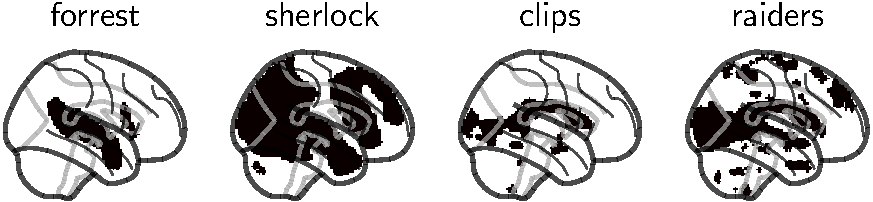
\includegraphics[width=\textwidth]{figures/mvica/reconstruction_score_roi.pdf}
  \caption{\textbf{Data-driven choice of ROI} Chosen ROIs for the experiment: Reconstructing the BOLD signal of missing subjects.}
  \label{fig:roi}
\end{figure}

The ROI choice is driven by the performance of Concat ICA (more information
available in appendix~\ref{brainmaps}.
\subsubsection{Datasets}

We use five fMRI datasets of subjects exposed to naturalistic stimuli. When needed, datasets are preprocessed with FSL \url{http://fsl.fmrib.ox.ac.uk/fsl} using slice time correction, spatial realignment, coregistration to the T1 image and affine transformation of the functional volumes to a template brain (MNI). Using Nilearn \cite{abraham2014machine}, preprocessed data are resampled, masked (using a full brain mask available at \url{http://cogspaces.github.io/assets/data/hcp_mask.nii.gz}), detrended and standardized after a 5 mm smoothing is applied.  
%
\paragraph{SHERLOCK}
In the SHERLOCK dataset, 17 participants are watching "Sherlock" BBC TV show (episode 1). 
%
These data are downloaded from \url{http://arks.princeton.edu/ark:/88435/dsp01nz8062179}. 
%
Data were acquired using a 3T scanner with an isotropic spatial resolution of 3 mm. 
%
More information including the preprocessing pipeline is available in \cite{sherlock}.
%
Subject 5 is removed because of missing data leaving us with 16 participants.
%
Although SHERLOCK data contains originally only 1 run, we split it into 4 blocks of 395 timeframes and one block of 396 timeframes for the needs of our experiments. 


\paragraph{FORREST}
In the FORREST dataset, 20 participants are listening to an audio version of the movie Forrest Gump.
%
FORREST data are downloaded from OpenfMRI \cite{poldrack2013toward}. 
%
Data were acquired using a 7T scanner with an isotropic spatial resolution of 1 mm (see more details in \cite{hanke2014high}.
%
More information about the forrest project can be found at \url{http://studyforrest.org}.
%
Subject 10 and run 8 are discarded because of missing data.
%
We therefore use full brain data of 19 subjects split in 7 runs of respectively 451, 441, 438, 488, 462, 439 and 542 timeframes.
 
\paragraph{RAIDERS}
In the RAIDERS dataset, 10 participants are watching the movie "Raiders of the lost ark".
% 
The RAIDERS dataset pertains to the Individual Brain Charting dataset (\cite{ibc}).\textbf{XXX}
% 
They were acquired at NeuroSpin using a 3T scanner with an isotropic spatial resolution of 1.5 mm.
% 
The RAIDERS dataset reproduces the protocol described in \cite{haxby2011common}.
%
We use full brain data of 10 subjects split in 9 runs of respectively 374, 297, 314, 379, 347, 346, 350, 353 and 211 timeframes.

\paragraph{CLIPS}
In the CLIPS dataset, 10 participants are exposed to short clips. 
%
The CLIPS dataset also pertains to the Individual Brain Charting dataset (\cite{ibc}).
%
It reproduces the protocol of original studies described in \cite{nishimoto2011reconstructing} and \cite{huth2012continuous}.
%
In our experiments we use the data of 10 participants acquired in 17 runs of 325 timeframes.

At the time of writing, the CLIPS and RAIDERS dataset from the individual brain charting dataset \url{https://project.inria.fr/IBC/} are not yet public, but they will be in the future. Protocols on the visual stimuli presented are available in a dedicated repository on Github: \url{https://github.com/hbp-brain-charting/public_protocols}. The informed consent of all subjects was obtained before scanning.

\paragraph{CamCAN}
In CamCAN dataset, 647 participants aged from 18 to 88 years are watching Alfred Hitchcock's "Bang! You're Dead" (edited so that it lasts only 8 minutes).
%
CamCAN consists of data obtained from the CamCAN repository (available at \url{http://www.mrc-cbu.cam.ac.uk/datasets/camcan/}) (see \cite{taylor2017cambridge} and \cite{shafto2014cambridge}).
%
We use all available subjects and runs yielding 647 participants and 1 run of 193 timeframes.

A summary about the size of each dataset is available in Table~\ref{tab:dataset_desc}.


\section{fMRI experiments}
\label{sec:app_expts}
\subsection{Dataset description and preprocessing}
\label{preprocessing}
\textbf{XXX Hum this repeats the rpevious section}
The full brain mask used to select brain regions is available in the Python package associated with the paper.

\paragraph{Sherlock}
In \emph{sherlock} dataset, 17 participants are watching "Sherlock" BBC TV show (beginning of episode 1). 
%
These data are downloaded from \url{http://arks.princeton.edu/ark:/88435/dsp01nz8062179}. 
%
Data were acquired using a 3T scanner with an isotropic spatial resolution of 3 mm. 
%
More information including the preprocessing pipeline is available in~\cite{chen2017shared}.
%
Subject 5 is removed because of missing data leaving us with 16 participants.
%
Although \emph{sherlock} data are downloaded as a temporal concatenation of two runs, we split it manually into 4 runs of 395 timeframes and one run of 396 timeframes so that we can perform 5 fold cross-validation in our experiments.


\paragraph{FORREST}
In FORREST dataset 20 participants are listening to an audio version of the Forrest Gump  movie.
%
FORREST data are downloaded from OpenfMRI~\cite{poldrack2013toward}. 
%
Data were acquired using a 7T scanner with an isotropic spatial resolution of 1~mm (see more details in~\cite{hanke2014high}) and resampled to an isotropic spatial resolution of 3~mm.
%
More information about the forrest project can be found at \url{http://studyforrest.org}.
%
Subject 10 is discarded because not all runs available for other subjects were available for subject 10 at the time of writing.
%
Run 8 is discarded because it is not present in most subjects.
 
\paragraph{RAIDERS}
In RAIDERS dataset, 11 participants are watching the movie "Raiders of the lost ark".
% 
The RAIDERS dataset belongs to the Individual Brain Charting dataset~\cite{ibc}.
% 
Data were acquired using a 3T scanner and resampled to an isotropic spatial resolution of 3~mm.
% 
The RAIDERS dataset reproduces the protocol described in~\cite{haxby2011common}.
%
Preprocessing details are described in~\cite{ibc}.

\paragraph{CLIPS}
In CLIPS dataset, 12 participants are exposed to short video clips. 
%
The CLIPS dataset also belongs to the Individual Brain Charting dataset (\cite{ibc}).
%
Data were acquired using a 3T scanner and resampled to an isotropic spatial resolution of 3~mm.
%
It reproduces the protocol of original studies described in \cite{nishimoto2011reconstructing} and \cite{huth2012continuous}.
%
Preprocessing details are described in~\cite{ibc}.

At the time of writing, the CLIPS and RAIDERS dataset from the individual brain charting dataset \url{https://project.inria.fr/IBC/} are available at \url{https://openneuro.org/datasets/ds002685}.
%
Protocols on the visual stimuli presented are available in a dedicated repository on Github: \url{https://github.com/hbp-brain-charting/public_protocols}.


\subsubsection{fMRI reconstruction: Evaluate the ability to recover BOLD signal on left-out runs}
\label{reconstruction}

When subjects are exposed to the same stimuli, SRM algorithms posit that the recorded fMRI data can be modeled as a product of two matrices, one of which is fixed across time but subject-specific (the spatial components) while the other varies across time but is common to all subjects (the shared response).
%
Under this framework, once spatial components are known, we can generate an accurate estimation of the data of one subject given the data of all others.
%
In this experiment we test whether we can recover data of a left-out subject using previous data of the same subject as well as data from other subjects. 
We denote $\mathbf{X}^{(-s)}$ brain recordings of all runs but run $s$:
 \begin{equation*}
	 \mathbf{X}^{(-s)} = 
\begin{bmatrix}
	\mathbf{X}^{(1)} \\
	\vdots \\
	\mathbf{X}^{(s-1)} \\
	\mathbf{X}^{(s+1)} \\
	\vdots \\
	\mathbf{X}^{(m)}
\end{bmatrix}
\end{equation*}

Similarly, $\mathbf{X}_i^{(-s)}$ refers to the brain recordings of subject $i$ using all runs but run $s$. The data from all subjects but $i$ acquired during run $s$ are denoted:
\begin{equation*}
	\mathbf{X}^{(s)}_{-i} = 
\begin{bmatrix}
	\mathbf{X}_1^{(s)} & \cdots & \mathbf{X}^{(s)}_{i-1} & \mathbf{X}^{(s)}_{i+1} & \cdots & \mathbf{X}^{(s)}_{n} 
\end{bmatrix}
\end{equation*}

We evaluate our model using a cross validation scheme known as co-smoothing (see \cite{wu2018learning}). First, all brain recordings for all runs but one $\mathbf{X}^{(-s)}$ are used for learning subjects spatial components $\mathbf{W}^{(-s)}$. The exponent in $\mathbf{W}^{(-s)}$ indicates that these spatial components were learned using all runs but run $s$. 

\begin{equation*}
	\mathbf{W}^{(-s)}, \mathbf{S}^{(-s)} = SRM(\mathbf{X}^{(-s)})
\end{equation*}

Then we focus on the left-out run $s$ and use all subjects but one $\mathbf{X}^{(s)}_{-i}$ to compute a shared response for the left-out run $\mathbf{S}^{(s)}$.

\begin{equation*}
	\mathbf{S}^{(s)} = \frac{\sum_{z=1, z\neq i}^n \mathbf{X}^{(s)}_z\mathbf{W}^{(-s)^T}_z}{n - 1}
\end{equation*}

From $\mathbf{S}^{(s)}$ and $\mathbf{W}_i^{-s}$ we compute $\widetilde{\mathbf{X}}^{(s)}_i$ which stands as an estimate of brain activity of the left-out subject $i$ during the left-out run $s$.

\begin{equation*}
	\widetilde{\mathbf{X}}_i^{(s)} = \mathbf{W}^{(-s)}_i \mathbf{S}^{(s)}
\end{equation*}


\begin{figure}
\centering
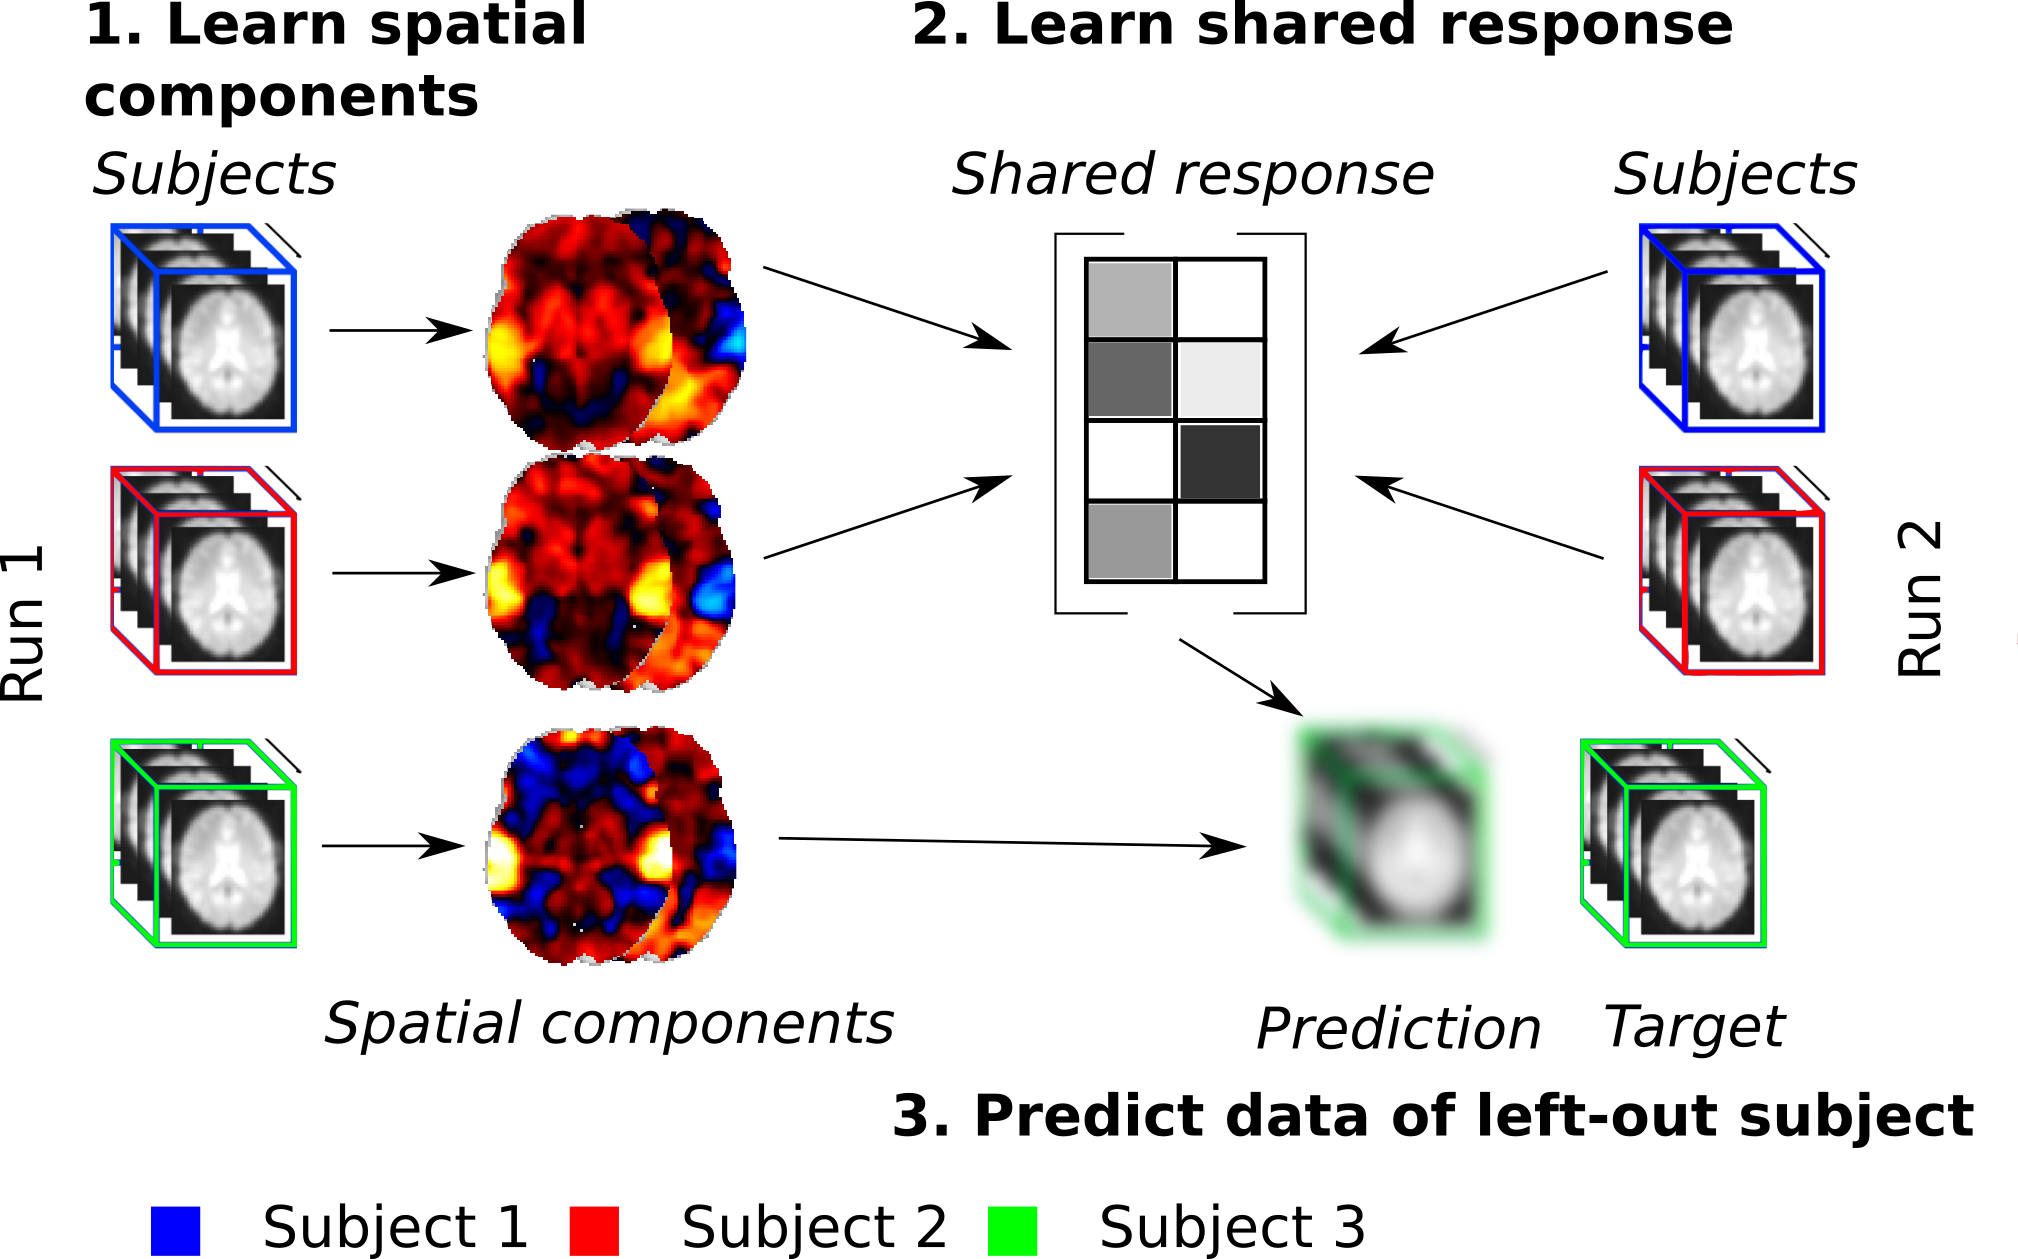
\includegraphics[scale=0.24]{figures/srm/conceptual_figure41.png}
\caption{\textbf{Experiment — Reconstruct data from a left-out subject} All runs but one are used to compute spatial components for every subject (left).
  %
  Then spatial components and data from the left-out run of all subjects but one are used to compute the shared response in the left-out run.
  %
  At last, the shared response during the left-out run and  the spatial components of the test subject are used to predict the data of the test subject in the left-out run.
  %
  The performance of the model is measured by comparing the prediction and true data using the $R^2$ score.}
\label{fig:experiment_reconstruction}
\end{figure}


An illustration of our reconstruction experiment is available in Figure~\ref{fig:experiment_reconstruction}.
%
The performance is measured voxel-wise using the $R^2$ score between $\widetilde{\mathbf{X}}_i^{(s)}$ and $\mathbf{X}_i^{(s)}$ as a similarity measure.
For any two time-courses $x \in \mathbb{R}^t$ and $y \in \mathbb{R}^t$ we define the $R^2$ score by:

\[
	R^2(x, y) = 1 - \frac{\sum_{z=1}^t (x[z] - y[z])^2}{\sum_{z=1}^t (y[z] - \overline{y}[z])^2} 
\]

Where $\overline{y} = \frac{1}{t}\sum_{z=1}^t y[z]$.
%
Following the leave-one-out cross validation scheme, all our experiments are done several times with a different left-out subject to reconstruct. 
%
We measure the average $R^2$ score across  all left-out subjects. Note that we obtain one such value per voxel.

\subsubsection{Predict age from spatial components}
Since spatial components are subject-specific they should be predictive of subject-specific features such as age.
%
In this experiment we try to predict subject's age from movie-watching data using SRM algorithms.
%
Functionally matched spatial components are obtained using an SRM algorithm.
%
They are divided into two groups (train and test data) where the train set contains 80\% of the data and the test set 20\%.
%
Within the train set we split again our data into two groups: the first group is used to train one Ridge model per spatial components, the second group is used to train a Random Forest to predict age from Ridge predictions. This way of stacking models is similar to the pipeline used in \cite{rahim2017joint}.
%
We use 5 fold cross validation to split the train set (so that the number of samples used to train the Random Forest is the number of elements in the train set).
%
Then the train set is used to train one Ridge model per spatial component.
%
On the test set each Ridge model makes a prediction and the predictions are aggregated using the Random Forest model.
%
An illustration of the process is available in Figure~\ref{fig:experiment_age_prediction}. 

In each Ridge model, the coefficient that determines the level of l2 penalization is set by generalized cross validation, an efficient form of leave-one-out cross validation (see the RidgeCV implementation of Scikit Learn \cite{pedregosa2011scikit}).

The train and test sets are chosen randomly. 5 different choices for the train and test set are made. We report the average mean absolute error (MAE) on the test set averaged over the 5 splits.

\begin{figure}
\centering
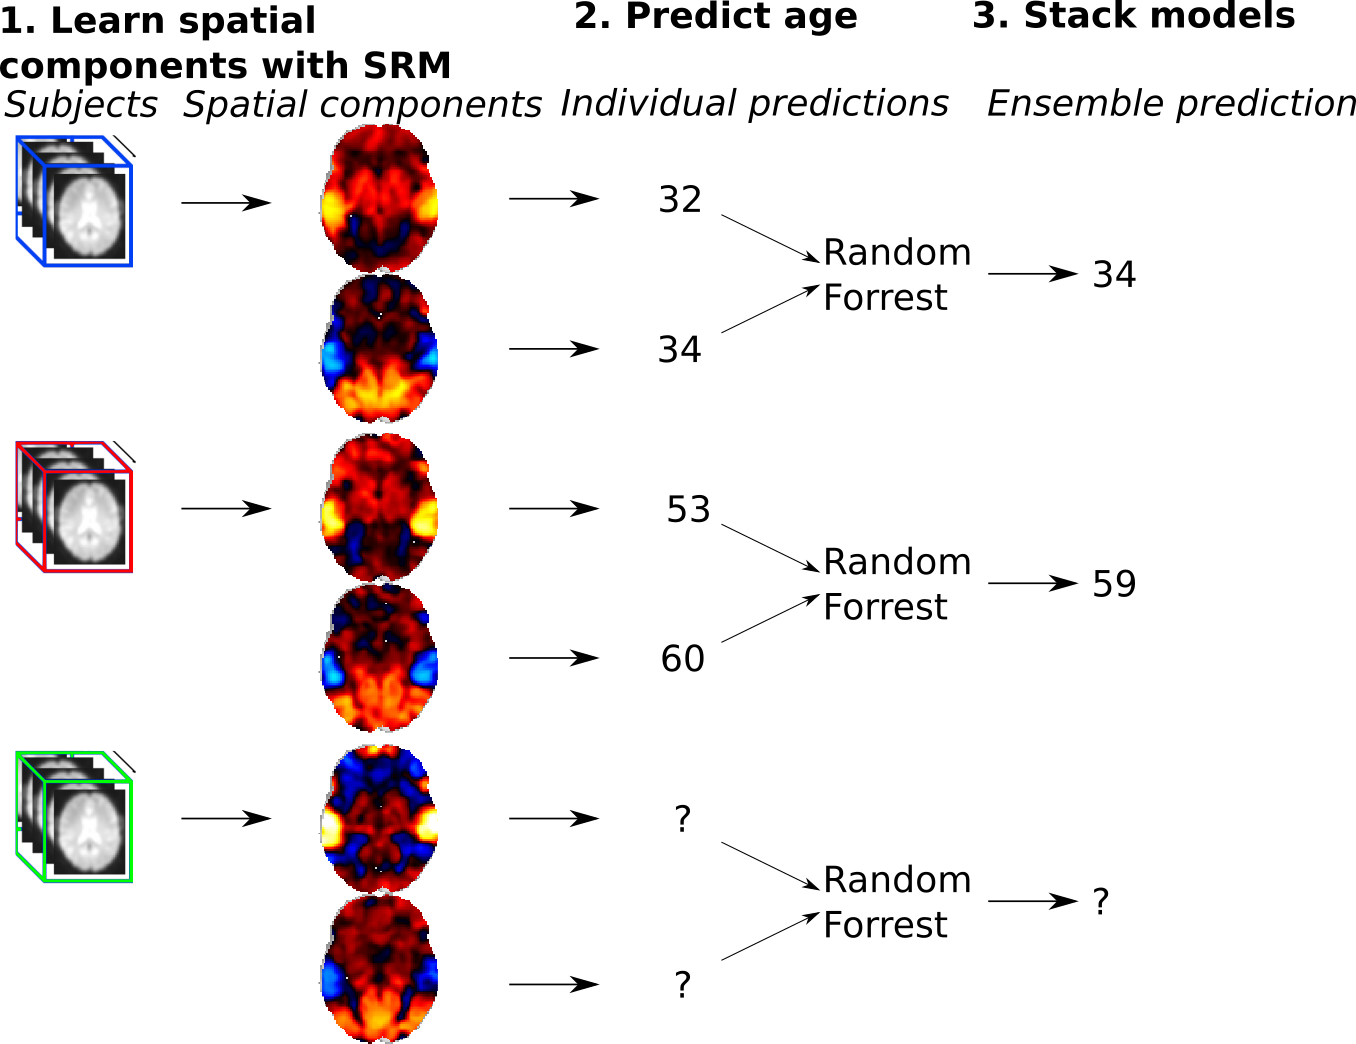
\includegraphics[scale=0.35]{figures/srm/conceptual_figure72.png}
\caption{\textbf{Experiment — Predict age from spatial components extracted using FastSRM}: We first learn the spatial components from fMRI data using SRM. We learn one Ridge model per spatial components to predict age across subjects. Then, these models are aggregated using a Random Forest (like in \cite{rahim2017joint}).} 
\label{fig:experiment_age_prediction}
\end{figure}


\section{Results and Discussion}

\subsection{fMRI Reconstruction}
We perform the reconstruction experiment on the FORREST, CLIPS, RAIDERS and SHERLOCK datasets. We compare brainiak's implementation of ProbSRM / DetSRM to our implementation of FastSRM in terms of fitting time, memory usage and performance. In order to be fair, we do not use parallelization ($n_{jobs} = 1$) and we set the number of iterations to 10 ($n_{iter}=10$) which is ProbSRM's default. Note that the fitting time of ProbSRM is roughly proportional to the number of iterations while it has a limited impact on the fitting time of FastSRM. 


We run our experiments on the full brain and report an $R^2$ score per voxel.
%
However we measure the performance in terms of mean $R^2$ score inside a region of interest (in order to leave out regions where there is no useful information).
%
In order to determine the region of interest, we focus on the results of ProbSRM with $10, 20, 50$ and $100$ components and keep only the intersection of regions where the $R^2$ score is above $0.05$.
%
This means of selecting regions favors ProbSRM. For completeness, full brain $R^2$ images obtained on the four datasets with ProbSRM and FastSRM using $20$ components averaged across subjects are available in Figure~\ref{fig:example_r2}.

In Figure~\ref{fig:mean_r2_score}, we plotted the mean $R^2$ score against the number of components ($k$) for ProbSRM, DetSRM and FastSRM algorithm with different atlases.
%
The $R^2$ score tends to increase with the number of components (which is what is expected as more information can be retrieved when the number of components is high).
%
FastSRM matches the performance of ProbSRM and DetSRM. This holds for any atlas we chose (BASC (444 parcels), SHAEFFER (800 parcels), MODL (512 and 1024 parcels)) and for all datasets we tried (SHERLOCK, RAIDERS, CLIPS and FORREST). 

In Figure~\ref{fig:fit_time}, we compare the running time of FastSRM, DetSRM and ProbSRM on the four different datasets.
%
FastSRM is on average (across datasets) about 5 times faster.
%
On the FORREST dataset, we compute a shared response in about 3 minutes when it takes about 20 minutes with ProbSRM or DetSRM.

In Figure~\ref{fig:memory_usage}, we compare the memory (RAM) consumption of FastSRM, DetSRM and ProbSRM on the four different datasets.
%
FastSRM is 20 to 40 times more memory friendly than ProbSRM and 10 to 20 times more memory friendly than DetSRM. On the FORREST dataset the memory usage of FastSRM is between 1 and 3 Go depending on the number of components and the atlas used. Most modern laptops meet these requirements. On the same dataset memory consumption is about 80 Go for ProbSRM and 40 Go for DetSRM which is manageable but costly for small labs.
%
Overall FastSRM yields same performance as ProbSRM and DetSRM while being much faster and using far less memory. We also show that the atlas used to reduce the data only has a minor impact on performance.

\begin{figure}
\centering
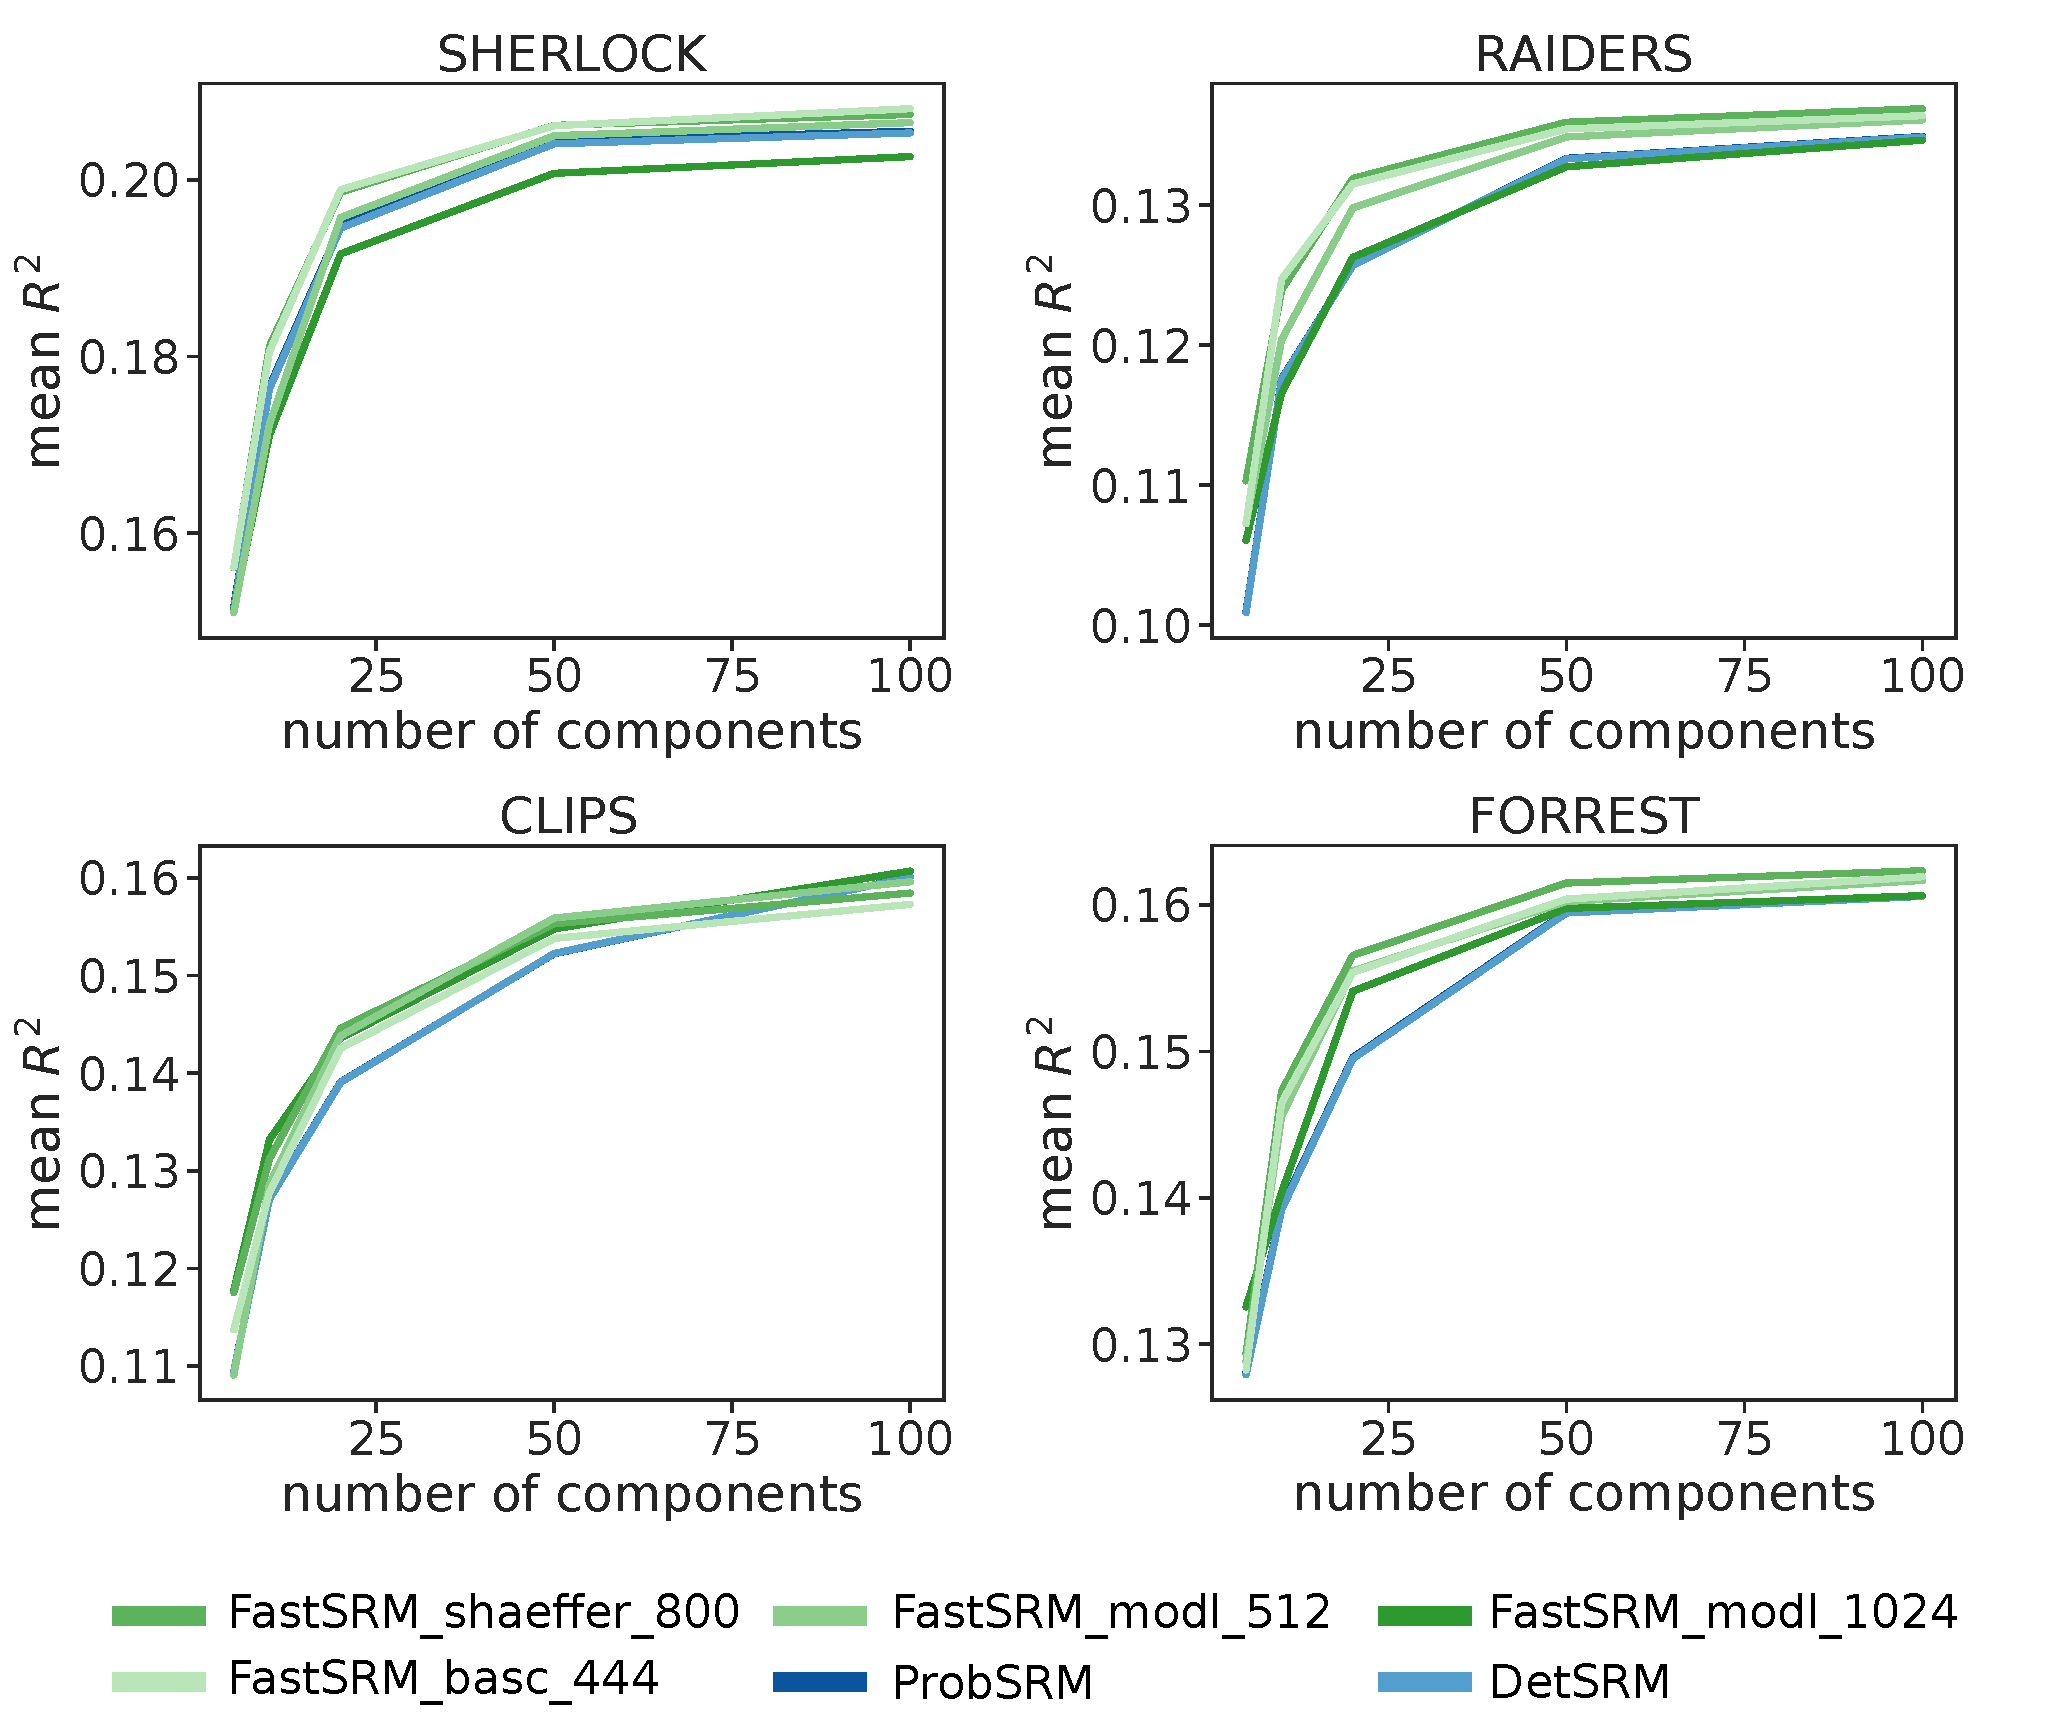
\includegraphics[scale=0.34]{figures/srm/perfs.pdf}
\caption{\textbf{Performance of the methods in an encoding test} We compare the performance (measured in terms of average $R^2$ score in a region of interest) of ProbSRM and FastSRM with different atlases in function of the number of components used. Atlases tested are MODL with 512 and 1024 parcels, Basc with 444 parcels and Shaeffer with 800 parcels. Datasets tested are SHERLOCK (top left), RAIDERS (top right), CLIPS (bottom left) and FORREST (bottom right). 
As we can see, no matter which atlas is chosen, FastSRM matches ProbSRM's performance.}
\label{fig:mean_r2_score}
\end{figure}

\begin{figure}
\centering
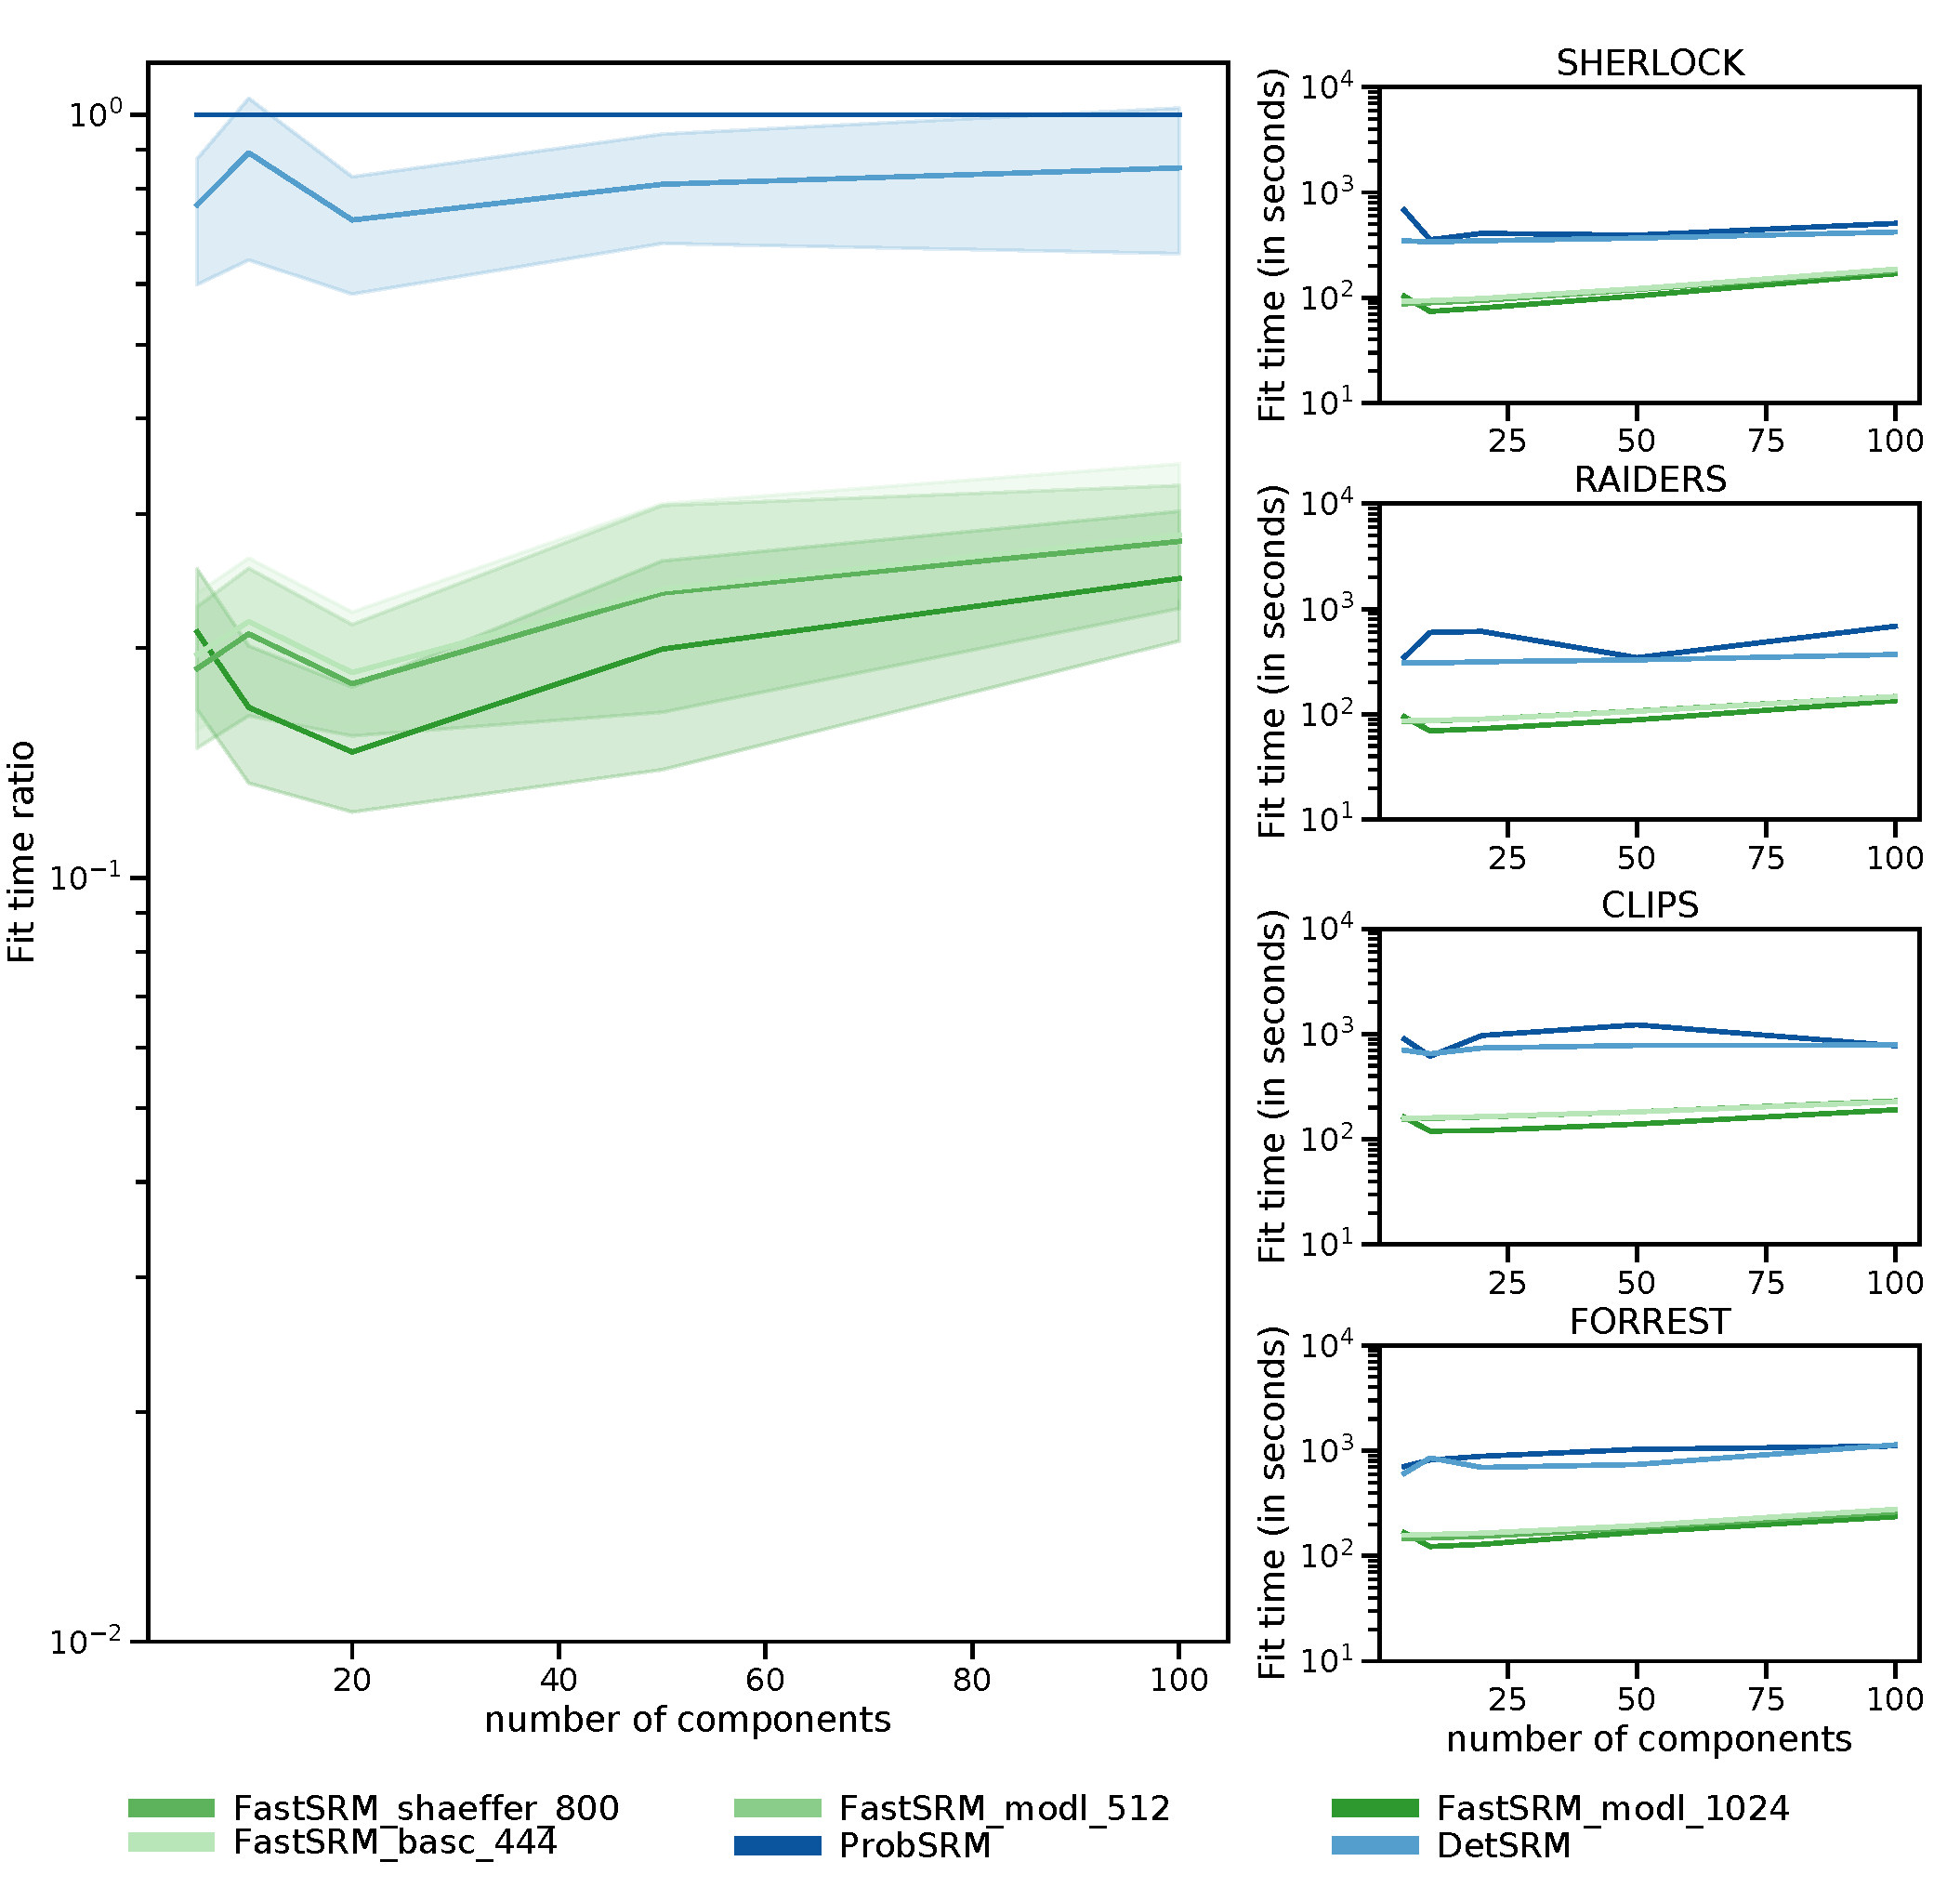
\includegraphics[scale=0.33]{figures/srm/fit_time.pdf}

\caption{\textbf{Fitting time of FastSRM, ProbSRM and DetSRM} We compare the fitting time of ProbSRM, DetSRM and FastSRM with different atlases in function of the number of components used. Atlases tested are MODL with 512 and 1024 parcels, Basc with 444 parcels and Shaeffer with 800 parcels. Datasets tested are SHERLOCK, RAIDERS, CLIPS and FORREST.
\textbf{Left}: Fitting time (as a fraction of ProbSRM fitting time) averaged over the four datasets.
\textbf{Right}: Fitting time (in seconds) for each of the four different datasets.
FastSRM is about 5 times faster than ProbSRM.
\textbf{XXX It is impossible to be sure of what we see hiven the 50 shades of green.}}
\label{fig:fit_time}
\end{figure}

\subsection{Predicting age from spatial components}
Because FastSRM is fast and memory efficient, it enables large-scale analysis of fMRI recordings of subjects exposed to the same naturalistic stimuli.
%
We use all 647 subjects of the CamCAN dataset and demonstrate the usefulness of FastSRM by showing that the spatial components that it extracts from movie watching data are predictive of age.
%
A key asset of FastSRM is that these spatial components can be visualized and therefore provide meaningful insights. 

Figure~\ref{fig:predict_age} shows that FastSRM predicts age with a good accuracy (better than ProbSRM and a lot better than chance) resulting in a mean absolute error (MAE) of 7.5 years.
%
It also shows that on CamCAN data, FastSRM is 4x faster and more than 150x more memory efficient than ProbSRM. As before and in order to ensure fair comparison the number of iterations is set to $10$ and we do not make use of parallelization. Note that the memory requirements of ProbSRM on the CamCAN dataset (186Go) make it difficult to use.
%
FastSRM does not suffer from memory issues, making it suitable to analyse big datasets.

A key asset of our pipeline is that we can see which spatial components are most predictive of age by using feature importance.
%
Feature importance is assessed by the Gini importance defined in \cite{breiman2001random} or \cite{louppe2013understanding}.
%
It measures for each feature the relative reduction in Gini impurity brought by this feature.
%
Feature importance varies with different splits. We use the averaged feature importance over the 5 splits of our pipeline.
%
In Figure~\ref{fig:predict_age} are shown the 3 most important spatial components representing respectively 16\%, 12\% and 8\% of total feature importance.
%
These spatial components in decreasing order of importance represent the visual dorsal pathway, the precuneus and the visual ventral pathway. 
%
The fact that averaged spatial components are interpretable and meaningful allows us to study the influence of age on brain networks involved in movie-watching.
%
In Figure~\ref{fig:predict_age_interpretation}, we plot the most important spatial component averaged within groups of ages.
%
We see that these spatial components evolve with age allowing us to visually identify which regions are meaningful. 
%
It turns out that aging is mostly reflected in brain activity as a
fading of activity in the spatial correlates of movie watching,
particularly in the dorsal visual cortex.
%
%With FastSRM, we can see how networks involved in movie-watching evolve with age. 


\begin{figure}
\centering
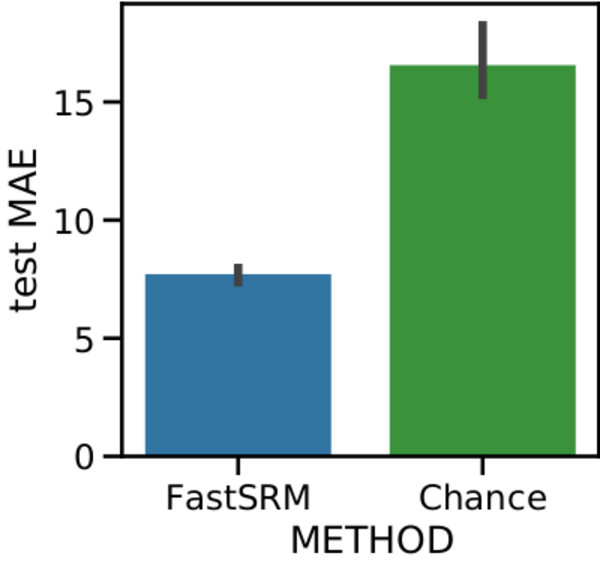
\includegraphics[scale=0.44]{figures/srm/predict_age.pdf}

\begin{tabular}{|c|c|c|}
	\hline
	Algorithm & Memory usage (in Go) & Fitting time (in minutes) \\
	\hline
	FastSRM & 1.1 & 15 \\
	ProbSRM & 186.3 & 69 \\
	\hline
\end{tabular}
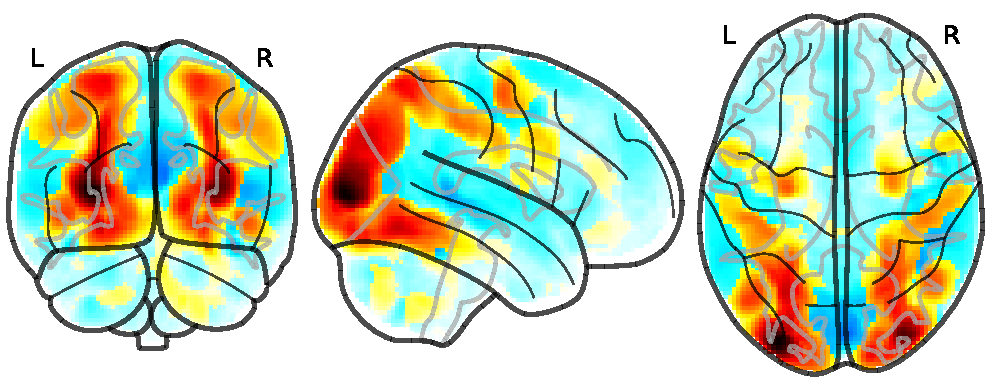
\includegraphics[scale=0.365]{./figures/srm/maps_feature_imp_0_16.pdf}
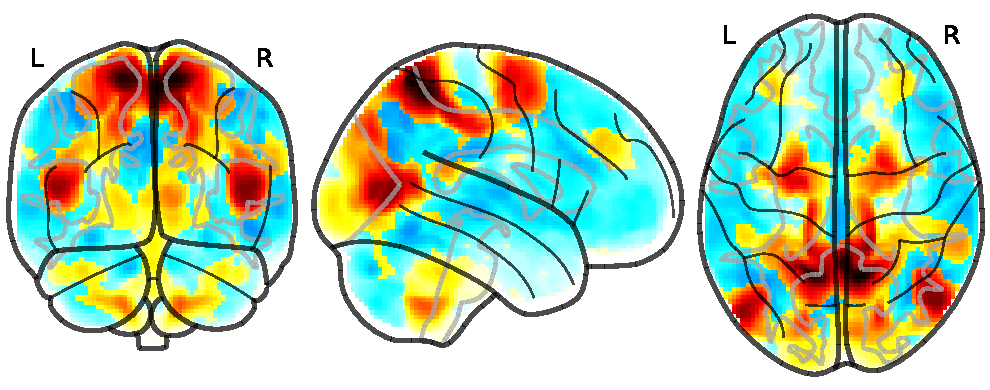
\includegraphics[scale=0.365]{./figures/srm/maps_feature_imp_0_12.pdf}
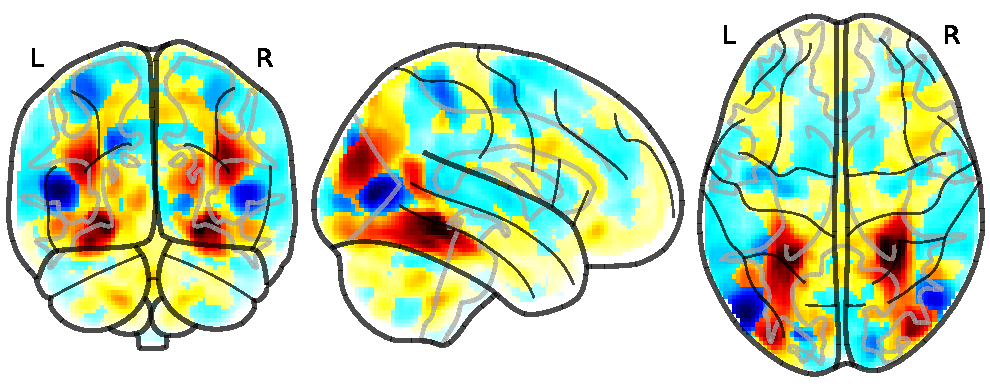
\includegraphics[scale=0.365]{./figures/srm/maps_feature_imp_0_08.pdf}

\caption{\textbf{Age prediction from spatial components}: (top) FastSRM predicts age with a good accuracy (better than ProbSRM and a lot better than chance) resulting in a mean absolute error (MAE) of 7.5 years. (middle) FastSRM is more than 4x faster than ProbSRM and uses 150x less memory, hence it scales better than ProbSRM. (bottom) The three most important spatial components in terms of the reduction in Gini impurity they bring (see Gini importance or Feature importance in \cite{breiman2001random}, \cite{louppe2013understanding}). From top to bottom, the most important spatial component (feature importance: 16\%) highlights the visual dorsal pathway, the second most important spatial component (feature importance: 12\%) highlights the precuneus and the third most important spatial component (feature importance: 8\%) highlights the visual ventral pathway.} 
\label{fig:predict_age}
\end{figure}

\begin{figure}
\centering
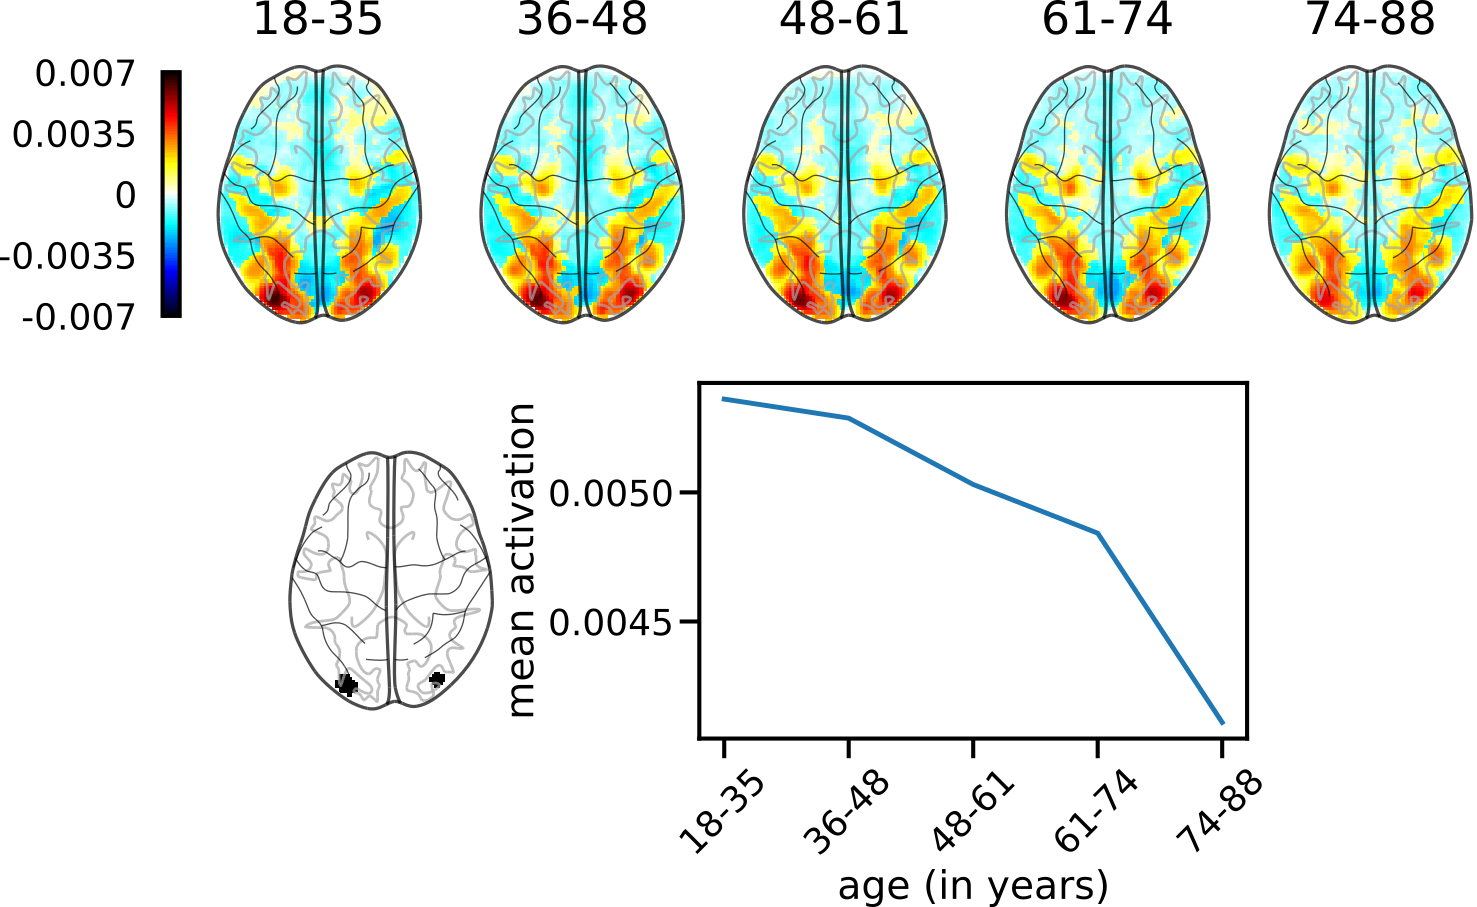
\includegraphics[scale=0.35]{figures/srm/feature_importance_age_prediction.png}
\caption{\textbf{Evolution of the most predictive spatial component with age}: (Top) Spatial component most predictive of age averaged within groups of different age (18-35, 36-48, 48-61, 61-74, 74-88). (Bottom) Mean activation in the region highlighted by the mask on the left. We see that the activity in the dorsal pathway decreases with age, which explains why this spatial component is a good predictor of age.}
\label{fig:predict_age_interpretation}
\end{figure}



\subsection{Conclusion}
As studies using naturalistic stimuli will tend to become more common and large within and across subjects, we need scalable models especially in terms of memory usage.
%
This is what FastSRM provides.
%
We show that while FastSRM matches the performance of ProbSRM or DetSRM, it is
significantly faster and requires a lot less memory. While FastSRM's scalability relies on the use of atlases to compress the BOLD signal, we show that the precise choice of the atlas has only marginal effects on performance.


FastSRM allows large scale analysis of fMRI data of subjects exposed to naturalistic stimuli. As one example of such analysis, we show that it can be used to predict age from movie-watching data. Interestingly, although FastSRM is an unsupervised model, it extracts meaningful networks and as such constitutes a practical way of studying subjects exposed to naturalistic stimuli.

We also show that individual information can be extracted from the fMRI activity when subjects are exposed to naturalistic stimuli. Our predictive model is reminiscent of that of \cite{bijsterbosch2018relationship}, that have shown that ICA components obtained from the decomposition of resting state data carry important information on individual characteristics. 
%

As a side note, we chose to keep the orthonormality assumptions of the original SRM model but slight modifications of our implementation of FastSRM would allow one to build more refined model promoting sparsity, non-negativity or smoothness of spatial components for example.

The remaining difficulty with SRM is to interpret the spatio-temporal decomposition. Reverse correlation \cite{hasson2004intersubject} can be used to clarify the cognitive information captured in the shared response.

Our code is freely available at \url{https://github.com/hugorichard/brainiak/tree/fastsrm}.


\part{MultiView ICA}
\label{part:mvica}
\chapter{MultiView ICA theory}
\label{ch:mvica1}
In the previous section, we have introduced a fast version of the shared
response model. While this provides a useful dimension reduction framework, it
assumes orthogonality of the mixing matrices which is not biologically
plausible.

In this section, we propose a novel group ICA method called \emph{MultiView ICA}.
In contrast to most Group ICA methods, MultiViewICA is grounded in a principled
probabilistic model of the problem and comes with statistical guarantees such as
asymptotic efficiency.

MultiViewICA models each subject's dataset as a linear combination of a common
components matrix with additive Gaussian noise.
% 
Importantly, we consider that the noise is on the components and not on
the sensors.
% 
This greatly simplifies the likelihood of the model which can even be
written in closed-form.

Despite its simplicity, MultiView ICA allows for an expressive representation of inter-subject variability through subject-specific functional topographies (mixing matrices) and variability in the individual response (with noise in the component domain).
% 
To the best of our knowledge, this is the first time that such a tractable likelihood is proposed for multi-subject ICA.
% 
The likelihood formulation shares similarities with the usual ICA likelihood, which allows us to develop a fast and robust alternate quasi-Newton method for its maximization.

We first introduce the MultiView ICA model, and show that it is identifiable. We then write its likelihood in closed form, and maximize it using an alternate quasi-Newton method.
%
We also provide a sensitivity analysis for MultiView ICA, and show that the choice of the noise parameter in the algorithm has little influence on the output.
\section{Multiview ICA for Shared response modelling}
\label{sec:mvica}
\subsection{Model, likelihood and approximation}
%
Given $m$ subjects, we model the data of subject $i$ as a random vector
$\xb_i\in\bbR^p$  such that:
\begin{equation}
\label{eq:ica_model}
    \xb_i = A_i(\sbb + \nb_i), \enspace i=1,\dots, m
\end{equation}
%\bt{Matrices as bold letters ?} \pa{I find it understandable to have nothing but matrices in uppercase}
where $\sbb \in \bbR^p$ are the shared independent components, $\nb_i \in \bbR^p$ is individual noise, $A_i \in \bbR^{p\times p}$ are the individual mixing matrices, assumed to be full-rank.
%
We assume that samples are observed i.i.d. For simplicity, we assume that the components share the same density $\delta$, so that the independence assumption is $p(\sbb) = \prod_{j=1}^p \delta(s_j)$. Finally, we assume that the noise is Gaussian decorrelated of variance $\sigma^2$, $\nb_i \sim \mathcal{N}(0, \sigma^2I_p)$, and that the noise is independent across subjects and independent from the components.
The assumption of additive white noise on the components models individual deviations from the shared components $\sbb$.
It is equivalent to having noise on the sensors with covariance $\sigma^2 A_i \left(A_i\right)^{\top}$, i.e. a scaled version of the data covariance without noise.

Since the components are shared by the subjects, there are many more observed variables than components in the model: there are $p$ components, while there are $p \times m$ observations.
%
Therefore, model~\eqref{eq:ica_model} can be seen as an instance of \emph{undercomplete} ICA.
%
The goal of multiview ICA is to recover the mixing matrices $A_i$ from observations of the $\xb_i$.
%
The following proposition extends the standard idenfitiability theory of ICA~\cite{comon1994independent} to multiview ICA, and shows that recovering the components/mixing matrices is a well-posed problem up to scale and permutation.
%
\begin{proposition}[Identifiability of MultiView ICA]
\label{prop:identifiability}
Consider $\xb_i, \enspace i=1\dots m,$ generated from~\eqref{eq:ica_model}. Assume that $\xb_i = A'_i(\sbb' + \nb'_i)$ for some invertible matrices $A'_i\in \bbR^{p\times p}$, independent non-Gaussian components $\sbb'\in \bbR^p$ and Gaussian noise $\nb'_i$. Then, there exists a scale and permutation matrix $P\in \bbR^{p\times p}$ such that for all $i$, $A'_i = A_i P$.
\end{proposition}
The proof is available in appendix~\ref{app:proof:mvica:identifiability}.

We propose a maximum-likelihood approach to estimate the mixing matrices. 
We denote by $W_i = (A_i)^{-1}$ the unmixing matrices, and view the likelihood
as a function of $W_i$ rather than $A_i$.

To derive the likelihood, we start by conditioning on $\sbb$. Then, we make a variable transformation from $\xb_i$ to $\nb_i=W_i\xb_i-\sbb$, as opposed to the transformation to $\sbb$ as is usual in ICA. Using the probability transformation formula, we obtain
\begin{equation}
p_{\xb_i|\sbb}(\xb_i|\sbb)=|W_i|p_{\nb_i}(W_i\xb_i-\sbb)    
\end{equation}
where $p_{\nb_i}$ is the density of $\nb_i$. Note that the $\xb_i$ are conditionally independent given $\sbb$, so we have:
\begin{equation}
  p_{\xb|\sbb}(\xb|\sbb)=\prod_{i=1}^m  |W_i| p_{\nb_i}(W_i\xb_i-\sbb)
\end{equation}
and we next get the joint density as:
\begin{equation}
  p_{\xb, \sbb}(\xb,\sbb)=p_{\sbb}(\sbb) \prod_{i=1}^m  |W_i| p_{\nb^i}(W_i\xb_i-\sbb)
\end{equation}

Integrating out $\sbb$ and taking the log gives the negative likelihood:
\begin{align} 
  \label{eq:likelihood}
 &\loss(W_1, \dots, W_m) =  \nonumber
  \\& -\sum_{i=1}^m\log|W_i| -  \log\left(\int_{\sbb}\exp\left(-\frac1{2\sigma^2}\sum_{i=1}^m\|W_i\xb_i - \sbb\|^2\right)p(\sbb)d\sbb\right)
\end{align}
up to additive constants.

The integral in~\ref{eq:likelihood} after factorization, is given by
\begin{equation}
\int_{\sbb} \prod_{j=1}^p \exp \left( -\frac{1}{2\sigma^2} \sum_{i=1}^m (W_{ij}^{\top}\xb_i-s_j)^2 \right) \delta(s_j) d\sbb
\end{equation}
where $W_{ij}$ is the $j$-th line of $W_i$. Denote $y_{ij}=W_{ij}^{\top}\xb_i$ and $\tilde{s_j}=\frac1m\sum_{i=1}^m y_{ij}$.  Fix $j$, and drop it to simplify notation. Then we need to solve the integral
\begin{align*}
   &\int_s \exp \left(-\frac{1}{2\sigma^2} \sum_{i=1}^m (y_i-s)^2 \right) \delta(s)ds\\
   &=\int_s \exp \left(-\frac{1}{2\sigma^2} [ m(\tilde{s}-s)^2 + \sum_{i=1}^m (y_i-\tilde{s})^2] \right) \delta(s)ds \\ 
&= \exp \left(-\frac{1}{2\sigma^2}\sum_{i=1}^m (y_i-\tilde{s})^2 \right) 
\int_z \exp \left(-\frac{m}{2\sigma^2} z^2 \right) \delta(\tilde{s}-z) dz
\end{align*}

where we have made the change of variable $z=\tilde{s}-s$. The remaining integral simply means that $\delta$ is smoothed by a Gaussian kernel, which can be computed exactly if $\delta$ is a Gaussian mixture. We therefore define $f(s) = -\log \left(\int_z \exp \left(-\frac{m}{2\sigma^2} z^2 \right) \delta(s-z) dz\right)$.

The negative log-likelihood becomes
\begin{equation}
    \label{eq:cost_function}
    \loss(W_1, \dots, W_m) = -\sum_{i=1}^m \log|W_i| + \frac1{2\sigma^2}\sum_{i=1}^m\|W_i\xb_i - \tilde{\sbb}\|^2 + f(\tilde{\sbb}).
\end{equation}
Multiview ICA is then performed by minimizing $\loss$, and the estimated shared components are $\tilde{\sbb}$.
The negative log-likelihood $\loss$ is quite simple, and importantly, can be computed easily given the parameters of the model and the data; it does not involve any intractable integral.
%

For one subject ($m=1$), $\loss(W_1)$ simplifies to the negative log-likelihood of ICA and we recover Infomax~\cite{bell1995information,cardoso1997infomax}, where the component log-pdf is replaced with the smoothened $f$.
%

\subsection{Alternate quasi-Newton method for MultiView ICA}
%
The parameters of the model are estimated by minimizing $\loss$.
%
We propose a combination of quasi-Newton method and alternate minimization for this task.
%
First, $\mathcal{L}$ is non-convex: it is only defined when the $W_i$ are invertible, which is a non-convex set.
%
Therefore, we only look for local minima as usual in ICA.
%
We propose an alternate minimization scheme, where $\loss$ is alternatively diminished with respect to each $W_i$. 
%
When all matrices $W_1, \dots, W_m$ are fixed but one, $W_i$, $\loss$ can be rewritten, up to an additive constant 
\begin{align}
    \label{eq:indiv_loss}
    &\loss_i(W_i) = \nonumber  \\&-\log|W_i| + \frac{1 - 1/m}{2\sigma^2}\|W_i\xb_i - \frac{m}{m-1}\tilde{\sbb}_{-i}\|^2 + f(\frac1m W_i \xb_i +\tilde{\sbb}_{-i}), 
\end{align}
with $\tilde{\sbb}_{-i} = \frac1m \sum_{j \neq i}W_j \xb_j$.
%
This function has the same structure as the usual maximum-likelihood ICA cost
function: it is written $\loss_i(W_i) = -\log|W_i| + g(W_i\xb_i)$, where $g(\yb)
= \sum_{j=1}^pf(\frac{y_j}{m} + \tilde{\sbb}_{-i, j}) + \frac{1 -
  1/m}{2\sigma^2}(y_j - \frac{m}{m-1}\tilde{\sbb}_{-i, j})^2$ where
$\tilde{\sbb}_{-i, j}$ is the $j$-th component of $\tilde{\sbb}_{-i}$.
%
Fast quasi-Newton algorithms ~\cite{zibulevsky2003blind, ablin2018faster} have been proposed for minimizing such functions.
%
We employ a similar technique as~\cite{zibulevsky2003blind}, which we now describe.

Quasi-Newton methods are based on approximations of the Hessian of $\loss_i$.
%
The relative gradient (resp. Hessian)~\cite{amari1996new, cardoso1996equivariant} of $\loss_i$ is defined as the matrix $G_i\in \bbR^{p \times p}$ (resp. tensor $\mathcal{H}_i \in \bbR^{p\times p\times p\times p}$) such that as the matrix $E\in\bbR^{p\times p}$ goes to $0$, we have $\loss_i((I_p + E)W_i) \simeq \loss_i(W_i) + \langle G_i, W_i\rangle + \frac12\langle E, \mathcal{H}_iE\rangle$. Standard manipulations yield:
\begin{equation}
    \label{eq:gradient}
    G_i = \frac1mf'(\tilde{\sbb})(\yb_i)^{\top} + \frac{1 - 1 /m}{\sigma^2}(\yb_i - \frac{m}{m-1}\tilde{\sbb}_{-i})(\yb_i)^{\top} - I_p 
\end{equation}
where $\yb_i= W_i\xb_i$.
\begin{align}
    \label{eq:hessian}
    (\mathcal{H}_i)_{abcd} &= \delta_{ad}\delta_{bc} + \delta_{ac}\left(\frac{1}{m^2}f''(\tilde{s}_a) + \frac{1 - 1/m}{\sigma^2}\right)y_{ib}y_{id} \\ &\text{for }a, b, c, d =1\dots p \nonumber
\end{align}

Newton's direction is then $-\left(\mathcal{H}_i\right)^{-1}G_i$. However, this Hessian is costly to compute (it has $\simeq p^3$ non-zero coefficients) and invert (it can be seen as a big $p ^2\times p^2$ matrix). Furthermore, to enforce that Newton's direction is a descent direction, the Hessian matrix should be regularized in order to eliminate its negative eigenvalues~\cite{nocedal2006numerical}, and $\mathcal{H}_i$ is not guaranteed to be positive definite.
%
These obstacles render the computation of Newton's direction impractical.
%
Luckily, if we assume that the signals in $\yb_i$ are independent, severall coefficients cancel, and the Hessian simplifies to the approximation
%\bt{IIUC if the sources are independent this is not an approximation} \pa{It is an approximation because even if the sources are independent, you have $y_i = s^i$ only when $W_i$ is the true unmixing matrix, i.e. when the algo has converged}
\begin{align}
    \label{eq:hessian_approx}
    (H_i)_{abcd} &= \delta_{ad}\delta_{bc} + \delta_{ac}\delta_{bd}\Gamma^i_{ab} \\
    &\text{with  }(\Gamma_i)_{ab} = \left(\frac{1}{m^2}f''(\tilde{s}_a) + \frac{1 - 1/m}{\sigma^2}\right)\left(y_{ib}\right)^2 \nonumber
\end{align}
This approximation is sparse: it only has $p(2p -1)$ non-zero coefficients.
%
In order to better understand the structure of the approximation, we can compute the matrix $\left(H_iM\right)$ for $M\in \bbR^{p\times p}$. 
%
We find $\left(H_iM\right)_{ab} = (\Gamma_i)_{ab}M_{ab} + M_{ba}$: $H_iM_{ab}$ only depends on $M_{ab}$ and $M_{ba}$, indicating a simple block diagonal structure of $H_i$.
%
The tensor $H_i$ is therefore easily regularized and inverted:
$\left((H_i)^{-1}M\right)_{ab} = \frac{\Gamma^i_{ba}M_{ab} - M_{ba}}{\Gamma^i_{ab}\Gamma^i_{ba} - 1}$.
%
Finally, since this approximation is obtained by assuming that the $\yb_i$ are independent, the direction $-H_i^{-1}G_i$ is close to Newton's direction when the $\yb_i$ are close to independence, leading to fast convergence.
%
Algorithm~\ref{algo:mv_ica} alternates one step of the quasi-Newton method for each subject until convergence.
%
A backtracking line-search is used to ensure that each iteration leads to a decrease of $\loss_i$.
%
The algorithm is stopped when the maximum norm of the gradients over one pass on each subject is below some tolerance level, indicating that the algorithm is close to a stationary point.

\begin{algorithm}[H]
\label{algo:mv_ica}
\SetAlgoLined
\KwIn{Dataset $(\xb_i)_{i=1}^m$, initial unmixing matrices $W_i$, noise parameter $\sigma$, function $f$,  tolerance $\varepsilon$}
Set tol$=+\infty$, $\tilde{\sbb} = \frac1m\sum_{i=1}^pW_i\xb_i$\\
 \While{\text{tol}$>\varepsilon$}{
 tol = 0 \\
  \For{$i=1\dots m$}{
  Compute $\yb_i = W_i \xb_i$, $\tilde{\sbb}_{-i} = \tilde{\sbb} - \frac1m\yb_i$, gradient $G_i$ (eq.~\eqref{eq:gradient}) and Hessian $H_i$ (eq.~\eqref{eq:hessian_approx})\\
  Compute the search direction $D = -H_i^{-1}G_i$\\
  Find a step size $\rho$ such that $\loss_i((I_p + \rho D)W_i) < \loss_i(W_i)$ with line search\\
  Update $\tilde{\sbb} = \tilde{\sbb} + \frac{\rho}{m} DW_i \xb_i$, $W_i = (I_p + \rho D)W_i$, tol$=\max($tol$,\|G_i\|)$\\
  }
 }
 \Return{Estimated unmixing matrices $W_i$, estimated shared components $\tilde{\sbb}$}
 \caption{Alternate quasi-Newton method for MultiView ICA}
\end{algorithm}
%
%
%
%
\subsection{Robustness to model misspecification}
Algorithm~\ref{algo:mv_ica} has two hyperparameters: $\sigma$ and the function $f$.
%
The latter is usual for an ICA algorithm, but the former is not.
%
We study the impact of these parameters on the separation capacity of the algorithm, when these parameters do not correspond to those of the generative model~\eqref{eq:ica_model}.
%
\begin{proposition}
\label{prop:robust}
We consider the cost function $\loss$ in eq.~\eqref{eq:cost_function} with noise parameters $\sigma$ and function $f$.
%
Assume sub-linear growth on $f'$: $|f'(x)|\leq c|x|^{\alpha} + d$ for some $c, d > 0$ and $0<\alpha<1$.
%
Assume that $\xb_i$ is generated following model~\eqref{eq:ica_model}, with noise parameter $\sigma'$ and density of the component $d'$ which need not be related to $\sigma$ and $f$.
%
Then, there exists a diagonal matrix $\Lambda$ such that $(\Lambda (A^1)^{-1}, \dots, \Lambda (A^m)^{-1})$ is a stationary point of $\loss$, that is $G^1,\dots, G^m =0$ at this point.
\end{proposition}
The proof is available in appendix~\ref{ref:robust}.

%
The sub-linear growth of $f'$ is a customary hypothesis in ICA which implies that $d$ has heavier-tails than a Gaussian, and in appendix~\ref{ref:robust} we provide other conditions for the result to hold.
%
In this setting, the shared components estimated by the algorithm are $\tilde{\sbb} = \Lambda (\sbb + \frac1m \sum_{i=1}^m \nb_i)$, which is a scaled version of the best estimate of the shared components under the Gaussian noise hypothesis.

This proposition shows that, up to scale, the true unmixing matrices are a stationary point for Algorithm~\ref{algo:mv_ica}: if the algorithm starts at this point it will not move.
%
The question of stability is also interesting: if the algorithm is initialized ~\emph{close} to the true unmixing matrices, will it converge to the true unmixing matrix?
%
In the appendix~\ref{sec:stability}, we provide an analysis similar to~\cite{cardoso1998blind}, and derive sufficient numerical conditions for the unmixing matrices to be local minima of $\mathcal{L}$.
%
We also study the practical impact of changing the hyperparameter $\sigma$ on the accuracy of a machine learning pipeline based on MultiviewICA on real fMRI data in the appendix Sec.~\ref{sec:app_sigma_impact}.
%
As expected from the theoretical study, the performance of the algorithm is barely affected by $\sigma$.

\section{Related Work}
In contrast to ConcatICA or GroupICA (see section~\ref{sec:canicaandconcatica}),
MultiView ICA maximizes a likleihood, which brings statistical guarantees like
consistency or asymptotic efficiency. Furthermore MultiViewICA finds individual
and shared independent components in a single step. This differs from ConcatICA or
GroupICA that require additional steps when individual components are needed
such as back-projection~\cite{calhoun2001method} or dual-regression~\cite{beckmann2009group}.

The approach of~\cite{guo2008unified} (see section~\ref{sec:guo}) optimizes the more
general model $\xb_i = A_i\sbb + \nb_i$. 
The likelihood for this model involves an intractable high dimensional integral
that is cumbersome to evaluate, and is then optimized with an EM algorithm using
an inexact E-step.
Having the simpler model $\xb_i = A_i(\sbb + \nb_i)$ leads to a closed-form likelihood,
that can then be optimized by more efficient means.
Note that in MultiView ICA, the noise can be interpreted as individual variability rather than sensor noise. %It offers a way to capture more structured noise as is often the case in brain signals.


The SR-ICA approach of \cite{zhang2016searchlight} performs dimension reduction, merging and independent component estimation. It is therefore similar to our method.
However, they propose to modify the FastICA algorithm~\cite{hyvarinen1999fast} in a rather heuristic way, without specifying an optimization problem, let alone maximizing a likelihood. In the experiments on fMRI data in appendix~\ref{appendix_reproduce}, we obtain better performance with MultiView ICA than the reported performance of SR-ICA.

One strength of our model is that we only assume that the mixing matrices are invertible and still enjoy identifiability whereas some other approaches impose additional constraints. For instance tensorial methods~\cite{beckmann2005tensorial} assume that the mixing matrices are the same up to diagonal scaling.
Other methods impose a common mixing matrix~\cite{cong2013validating, grin2010independent, calhoun2001fmri, Monti18UAI}. Like PCA, the Shared Response Model~\cite{chen2015reduced} (SRM) assumes orthogonality of the mixing matrices. While the model defines a simple likelihood and provides an efficient way to reduce dimension, the orthogonal constraint may not be plausible.

Deep Learning methods, such as convolutional auto-encoders (CAE), can also be used to find the subject specific unmixing~\cite{chen2016convolutional}. While these nonlinear extensions of the aforementioned methods are interesting, these models are hard to train and interpret. In the experiments on fMRI data in appendix~\ref{appendix_reproduce}, we obtain better accuracy with MultiView ICA than that of CAE reported in~\cite{chen2016convolutional}.

Lastly, IVA based methods (see section~\ref{sec:IVA}) do not specifically model
the shared response which is the quantity of interest in this work.

In the next section, we evaluate the performance of MultiView ICA on synthetic
data, on EEG and fMRI data and compare its performance to other GroupICA methods.
\chapter{MultiView ICA in practice}
\label{ch:mvica2}
In chapter~\ref{ch:mvica1}, we have introduced MultiViewICA and presented its
theoretical properties.
In this chapter, we empirically verify through extensive experiments on fMRI and
MEG data that MultiView ICA improves component identification with respect to competing methods, suggesting that the expressiveness and robustness of this model make it a useful tool for multivariate neural signal analysis.

\section{Experimental setting}
\label{sec:expts}
In the following, the noise parameter in MultiviewICA is always fixed to $\sigma =1$.
We use the function $f(\cdot)= \log\cosh(\cdot)$, giving $f'(\cdot) =
\tanh(\cdot)$ ($f'$ is called the learning function or non-linearity~\cite{hyvarinen1998independent}).
We use the Infomax cost function~\cite{bell1995information} with the same non-linearity to run standard ICA, with the Picard algorithm~\cite{ablin2018faster} for fast and robust minimization of the cost function. Picard is applied with the default hyper-parameters.
The code for MultiViewICA is available online at \url{https://github.com/hugorichard/multiviewica}.
%

We compare the following methods to obtain $p$ components:
\emph{PermICA} is described in section~\ref{sec:permica}.
%
\emph{SRM} is the FastSRM algorithm described in part~\ref{part:fastsrm}.
%
\emph{ConcatICA} is described in section~\ref{sec:canicaandconcatica}.
%
\emph{PCA+ConcatICA} corresponds to ConcatICA applied on subject data that have been first individually reduced by PCA with $p$ components. 
%
\emph{CanICA} is described in section~\ref{sec:canicaandconcatica}.
We define the chance level as the performance of an algorithm that computes unmixing matrices and projections to lower dimensional space by sampling random numbers from a standard normal distribution. 
% 


The dimension reduction in MultiView ICA and PermICA is performed with SRM in
fMRI experiments and subject-specific PCA in MEG experiments.

Since the cost function $\mathcal{L}$ is non-convex, having a good initialization can make a difference in the final result. We propose a two stage approach.
We begin by applying PermICA on the datasets, which gives us a first set of unimixing matrices $W_1, \dots, W_m$.
Note that we could also use ConcatICA for this task.
Next, we perform a diagonal scaling of the mixing matrices, i.e. we find the diagonal matrices $\Lambda_1, \dots, \Lambda_m$ such that $\mathcal{L}(\Lambda_1W_1, \dots, \Lambda_mW_m)$ is minimized.
To do so, we employ Algorithm~\ref{algo:mv_ica} but only take into account the diagonal of the descent direction at each step: the update rule becomes $W_i \leftarrow (I_p + \rho \text{Diag}(D))W_i$.
The initial unmixing matrices for Algorithm~\ref{algo:mv_ica} are then taken as $\Lambda_1W_1, \dots, \Lambda_mW_m$.
Empirically, we find that this two stage procedure allows the algorithm to start close to a satisfactory solution.
A summary of our quantitative results on real data is available in appendix~\ref{sec:app_real_data}.


\section{Synthetic experiment}

We validate our method on synthetic data generated according to the model in equation~\eqref{eq:ica_model}.
%
The components are generated i.i.d. from a Laplace density $d(x)=\frac12\exp(-|x|)$.
%
The mixing matrices $A_1,\cdots, A_m$ are generated with i.i.d. entries following a normal law.
Each compared algorithm returns a sequence of estimated unmixing matrices $W_1, \dots, W_m$.
%
The performance of an algorithm is measured by the reconstruction error between the estimated components and the true components.

\begin{figure}
  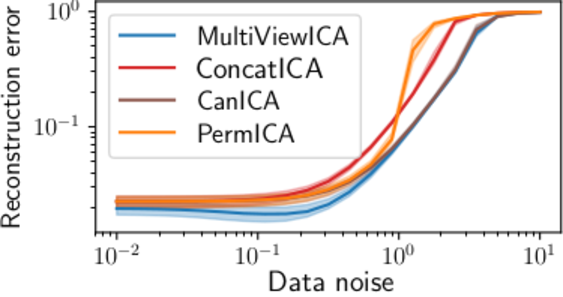
\includegraphics[width=0.5\textwidth]{figures/mvica/distance_expe.pdf}
  \captionof{figure}{\textbf{Synthetic experiment}: reconstruction error of the
    algorithms on data following model $\xb_i = A_i(\sbb + \nb_i)$.}
  \label{fig:mvica:synth}
\end{figure}

%$\frac1M\sum_{i=1}^Md(W^iA^i)$, where $d(P)=\sum_{i=1}^n \left(\sum_{j=1}^n\frac{|p_{ij}|}{\max_{p} |p_{ip}|} - 1\right) + \sum_{j=1}^n \left(\sum_{i=1}^n\frac{|p_{ij}|}{\max_{p} |p_{pj}|} - 1\right)$.
%
%This quantity cancels if and only if $P$ is a scale and permutation matrix.
%
We use $m=10$ datasets, $p=15$ components and $n=1000$ samples. Each experiment is repeated with $100$ random seeds.
%
We vary the noise level in the data generation from $10^{-2}$ to $10$ and
display the performance of algorithms in Figure~\ref{fig:mvica:synth}.

Multiview ICA has uniformly better performance than the other algorithms, which illustrates the strength of maximum-likelihood based methods. In accordance with results of section~\ref{sec:mvica}, it is able to separate the components even with misspecified noise parameter and component density.
%
%\subsection{fMRI experiments}
%\label{sec:experiments}


\section{fMRI experiments}
We use the \emph{Forrest}, \emph{Sherlock}, \emph{Raiders} and \emph{CLIPS} datasets described in section~\ref{srm:datasets:fmri}.

\subsection{Reconstructing the BOLD signal of missing subjects}
\label{sec:srm:reconstruction}
\label{reconstruction}
We want to show that once unmixing matrices have been learned, they can be
used to predict evoked responses across subjects. This can be used to perform
missing data imputation when the sessions of some subjects are missing.
In~\cite{zhang2018transfer}, the authors consider multiple fMRI datasets that
share a subpart of their subjects and use the fact that some subjects are shared
to transfer information across datasets. Our reconstruction experiment measures
a related quantity: the methods ability to predict data of left-out subjects
from other subjects.

In this experiment we apply a 6\,mm spatial smoothing to all datasets. 
We split the data into three groups. First, we randomly choose $80\%$ of all runs from all subjects to form the training set.
%
Then, we randomly choose $80\%$ of subjects and take the remaining $20\%$  runs as testing set.
%
The left-out runs  of the remaining subjects form the validation set.
%
The compared algorithms are run on the training set and evaluated using the testing and validation sets.
%
After an algorithm is run on training data, it defines for each subject a \emph{forward operator} that maps individual data to the space spanned by components and a \emph{backward operator} that maps the component space to individual data. For instance in ICA the forward operator is the product of the dimensionality reduction projection and unmixing matrix.
%
We estimate the shared responses on the testing set by applying the forward operators on the testing data and averaging. Finally, we reconstruct the individual data from subjects in the validation set by applying the backward operators to the shared responses. We measure the difference between the true signal and the reconstructed one using voxel-wise $R^2$ score. The $R^2$ score between two series $\xb \in \bbR^n$ and $\yb \in \bbR^n$ is defined as
$R^2(\xb, \yb) = 1 - \frac1{n\Var(\yb)}\sum_{t=1}^n (x_t - y_t)^2$, where $\Var(\yb) = \frac1n\sum_{t=1}^n (y_t - \frac1n \sum_{t'=1}^n y_{t'})^2$ is the empirical variance of $\yb$.
%
The $R^2$ score is always smaller than $1$, and equals $1$ when $\xb= \yb$.
The experiment is repeated 25 times with random splits to obtain error bars.

An illustration of our reconstruction experiment is available in Figure~\ref{fig:conceptual:reconstruction}.

\begin{figure}
  \centering
  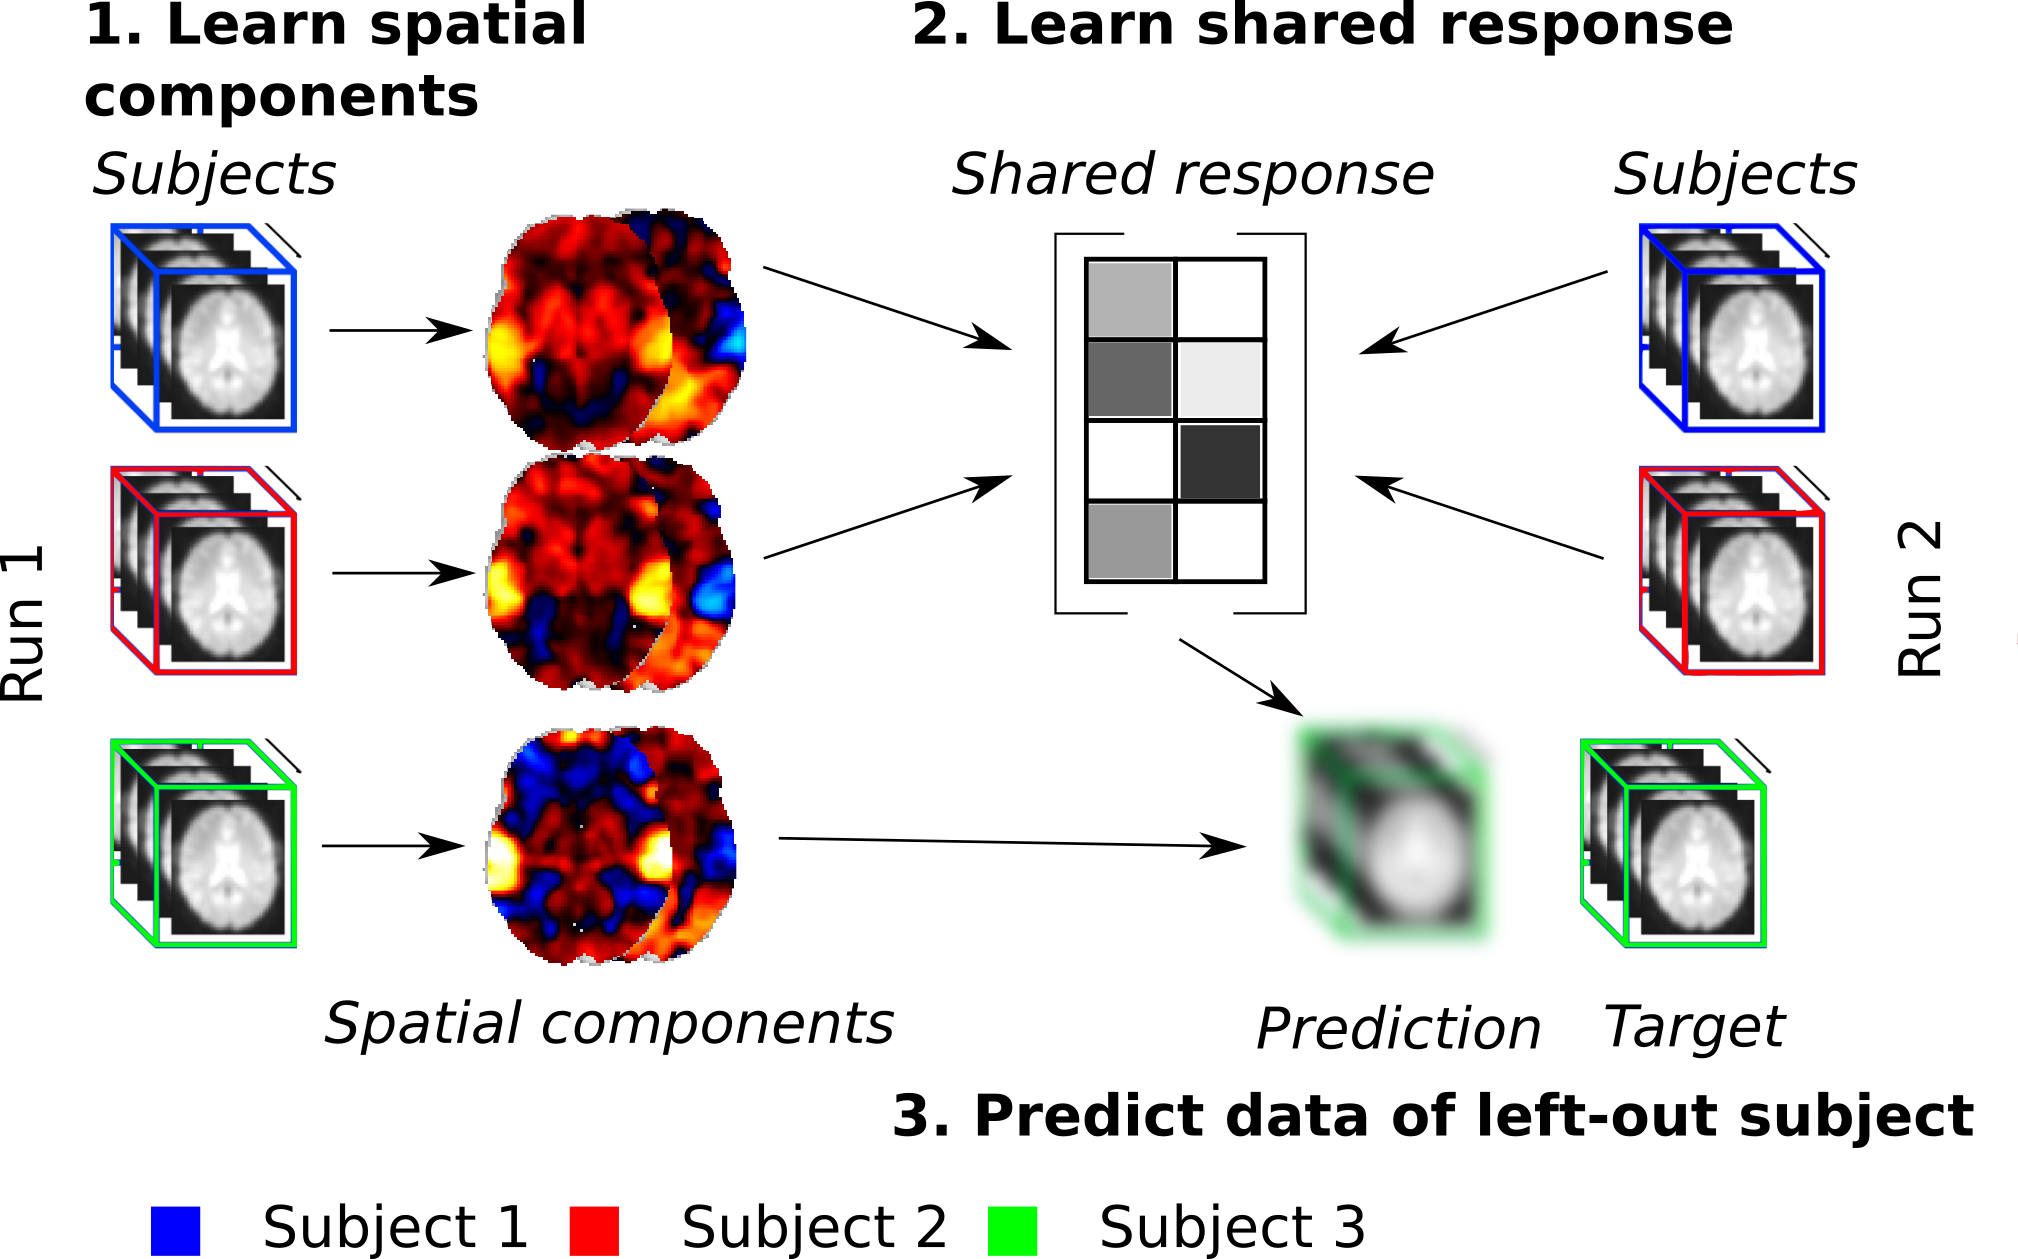
\includegraphics[scale=0.24]{figures/srm/conceptual_figure41.png}
  \caption{\textbf{Experiment — Reconstruct data from a left-out subject} All runs but one are used to compute spatial components for every subject (left).
    % 
    Then spatial components and data from the left-out run of all subjects but one are used to compute the shared response in the left-out run.
    % 
    At last, the shared response during the left-out run and  the spatial components of the test subject are used to predict the data of the test subject in the left-out run.
    % 
    The performance of the model is measured by comparing the prediction and true data using the $R^2$ score.}
  \label{fig:conceptual:reconstruction}
\end{figure}


The $R^2$ score per voxel depends heavily on which voxels are considered. For example voxels in the
visual cortex are better reconstructed in the \emph{sherlock} dataset than in
the \emph{forrest} dataset.

Performances are therefore given in terms of mean $R^2$ score inside a region of interest (ROI) in order to leave out regions where there is no useful information.

In order to determine the ROIs, we focus on the R2 score per voxel between the BOLD signal reconstructed by ConcatICA and the actual bold signal. We run ConcatICA with $10, 20$ and $50$ components and select the voxels that obtained a positive R2 score for all sets of components.
% 
We discard voxels with an R2 score above 80\% as they visually correspond to artefacts and apply a binary opening using a unit cube as the structuring element. The chosen regions are plotted in figure~\ref{fig:roi}.

\begin{figure}
  \centering
  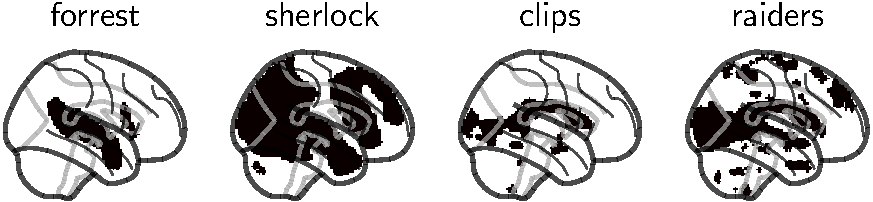
\includegraphics[width=\textwidth]{figures/mvica/reconstruction_score_roi.pdf}
  \caption{\textbf{Data-driven choice of ROI} Chosen ROIs for the experiment: Reconstructing the BOLD signal of missing subjects.}
  \label{fig:roi}
\end{figure}

In Figure~\ref{fig:mvica:reconstruction}
(top) we report the mean $R^2$ score within regions of interest.
%
MultiView ICA has similar or better performance than the other methods on all datasets.
%
This demonstrates its ability to capture inter-subject variability, making it a candidate of choice to handle missing data or perform transfer learning.

\begin{figure}
  \centering
  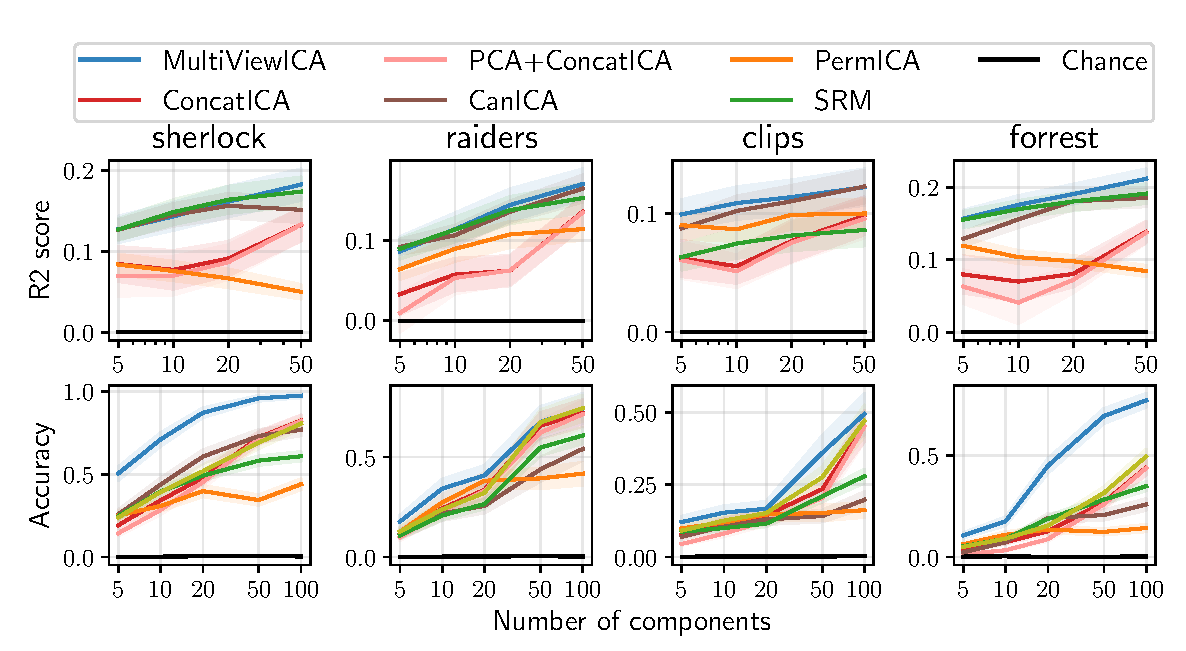
\includegraphics[width=0.9\textwidth]{figures/mvica/timesegment_matching_reconstruction.pdf}
  \caption{\emph{Top:} \textbf{Reconstructing the BOLD signal of
      missing subjects}. Mean $R^2$ score between reconstructed data and true
    data (higher is better). \emph{Bottom:} \textbf{Between subjects time-segment matching}. Mean
    classification accuracy. Error bars represent a 95 \% confidence interval over cross validation splits.}
  \label{fig:mvica:reconstruction}
  \label{fig:mvica:timesegment}
\end{figure}


For completeness, we plot in Figure~\ref{fig:brainmaps}, for ConcatICA, SRM and MultiViewICA, the R2 score per voxel using 50 components for datasets \emph{sherlock}, \emph{forrest}, \emph{raiders} and \emph{clips}. As could be anticipated from the task definition, \emph{forrest} obtains high reconstruction accuracy in the auditory cortices, while \emph{clips} shows good reconstruction in the visual cortex (occipital lobe mostly); the richer \emph{sherlock} and \emph{raiders} datasets yield good reconstructions in both domains, but also in other systems (language, motor).
%
We can also see that data reconstructed by MultiViewICA are
a better approximation of the original data than other methods.
%
This is particularly obvious for the \emph{clips} datasets where it is
clear that voxels in the posterior part of the superior
temporal sulcus are better recovered by MultiViewICA than by SRM or
ConcatICA.

\begin{figure}
  \centering
  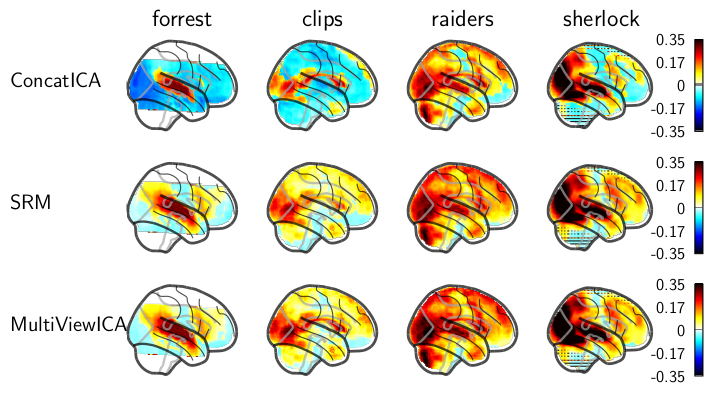
\includegraphics[width=\textwidth]{figures/mvica/reconstruction_score_fullbrain.png}
  \caption{\textbf{Reconstructing the BOLD signal of missing subjects: Reconstruction R2 score per voxel} We plot for ConcatICA, SRM and MultiViewICA, the R2 score per voxel using 50 components for datasets \emph{sherlock}, \emph{forrest}, \emph{raiders} and \emph{clips}. We can see that data reconstructed by MultiViewICA are more faithful reproduction of the original data than other methods.}
  \label{fig:brainmaps}
\end{figure}

%
\subsection{Between subjects time-segment matching} 
We reproduce the time-segment matching experiment described in
section~\ref{sec:timesegment_expe} and display the results in
Figure~\ref{fig:mvica:timesegment} (bottom). 
MultiView ICA yields a consistent and substantial improvement in accuracy compared to other methods on the four datasets. We see a marked improvement on the  sherlock and forrest datasets. A possible explanation lies in the preprocessing pipeline. Sherlock data undergo a 6~mm spatial smoothing and Forrest data are acquired at a higher resolution (7T vs 3T for other data). This affects the signal to noise ratio.
%

In order to investigate the practical impact of the choice of hyper-parameter
$\sigma$, we compute the accuracy of the MultiView ICA algorithm with different
choice of $\sigma$.
Results are reported in Fig.~\ref{fig:supp_noise_sensitivity}. 
\begin{figure}
  \centering
  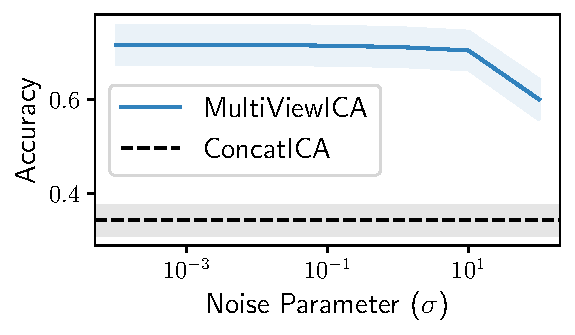
\includegraphics[width=0.6\textwidth]{figures/mvica/noise_sensitivity.pdf}
  \caption{\textbf{Effect of the parameter $\sigma$}: We compute the accuracy of the multiview-ICA pipeline on the time-segment matching experiment for various values of the $\sigma$ hyperparameter over a grid. The accuracy varies only marginally with $\sigma$.}
  \label{fig:supp_noise_sensitivity}
\end{figure}
MultiviewICA performs consistently well for a wide range of noise parameter values, and only breaks at very high values. It supports the theoretical claim issued in Prop~\ref{prop:robust} that the noise parameter is of little importance.

In appendix~\ref{sec:spatial_maps}, we plot the average forward operator across subjects of MultiView ICA and ConcatICA with 5 components on the forrest, sherlock, raiders and clips datasets.


\subsection{Between-runs time-segment matching}
\label{app_spatialmaps}
We measure the ability of each algorithm to extract meaningful shared components that correlate more when they correspond to the same stimulus than when they correspond to distinct stimuli. We use the \emph{raiders-full} dataset, which allows this kind of analysis because subjects watch some selected scenes from the movie twice, during the first two runs (1 and 2) and the last two (11 and 12).
%
First, the forward operators are learned by fitting each algorithm with 20 components on the data of all 11 subjects using all 12 runs. We then select a subset of 8 subjects and the shared components are computed by applying the forward operators and averaging.
%
We select a large target time-segment ($50$
timeframes) taken at random from run 1 and 2, and we try to localize the corresponding sample time-segment from the 10 last runs using a single component of the shared components.
%
The time-segment is said to be
correctly classified if the correlation between the target and corresponding sample
time-segment is higher than with any other time-segment (partially overlapping windows are excluded).
%
In contrast to the \emph{between subject time-segment matching} experiment, we obtain one accuracy score per component.
%
We repeat the experiment 10 times with different subsets of subjects randomly chosen and report the mean accuracy of the three best performing components in Figure~\ref{fig:swetha}. Error bars correspond to a 95~\% confidence interval.
%
MultiView ICA achieves the highest accuracy.

\begin{figure}
  \centering
  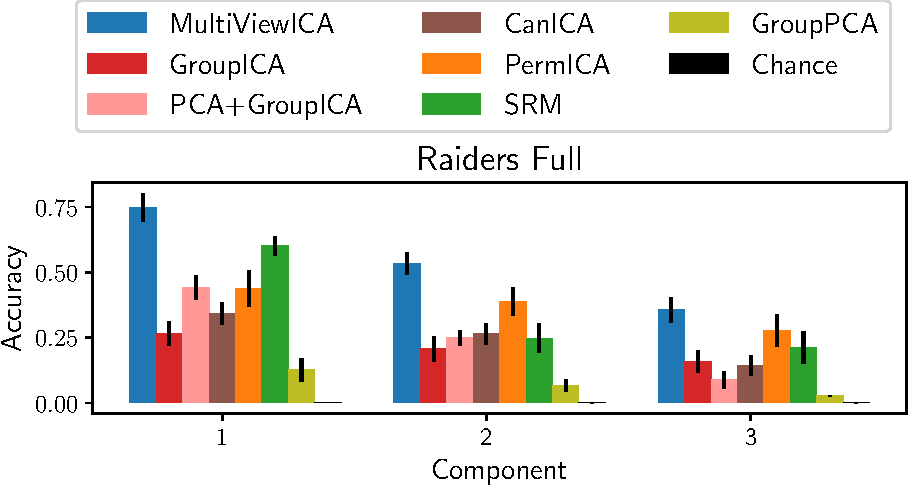
\includegraphics[width=\textwidth]{figures/mvica/swetha_exp_full_fit.pdf}
  \caption{\textbf{Between runs time-segment matching}. Interesting components correlates more when they correspond to the same stimulus (same scenes of the movie) than when they correspond to distinct stimuli (different scenes).
  %We show that when MultiView ICA is used, we can locate a target time-segment in one session using the data of another session corresponding to the same stimuli.
  We extract 20 components and report the mean accuracy of the three best performing components}
  \label{fig:swetha}
\end{figure}


We then focus on the 3 best performing components of MultiView ICA. For each component, we plot in Figure~\ref{fig:app_spatialmaps} (left) the shared components during two sets of runs where subjects were exposed to the same scenes of the movie. We then study the localisation of these components.
%
We average the forward operators across subjects and plot the columns corresponding to the components of interest in Figure~\ref{fig:app_spatialmaps} (right).
%
As each column is seen as a set of weights over all voxels, it represents a spatial map.

The component 1 of the shared responses follows almost the same pattern in the two set of runs corresponding to the same scenes of the movie. The spatial map corresponding to component 1 highlights the language network.
%
In component 2, the temporal patterns during the viewing of identical scenes are also very similar. The corresponding spatial map highlights the visual network especially the visual dorsal pathway.
%
In component 3, there exists a similarity however less striking than with the two previous components. The corresponding spatial map highlights a contrast between the spatial attention network and the auditory network.

\begin{figure}
  \centering
  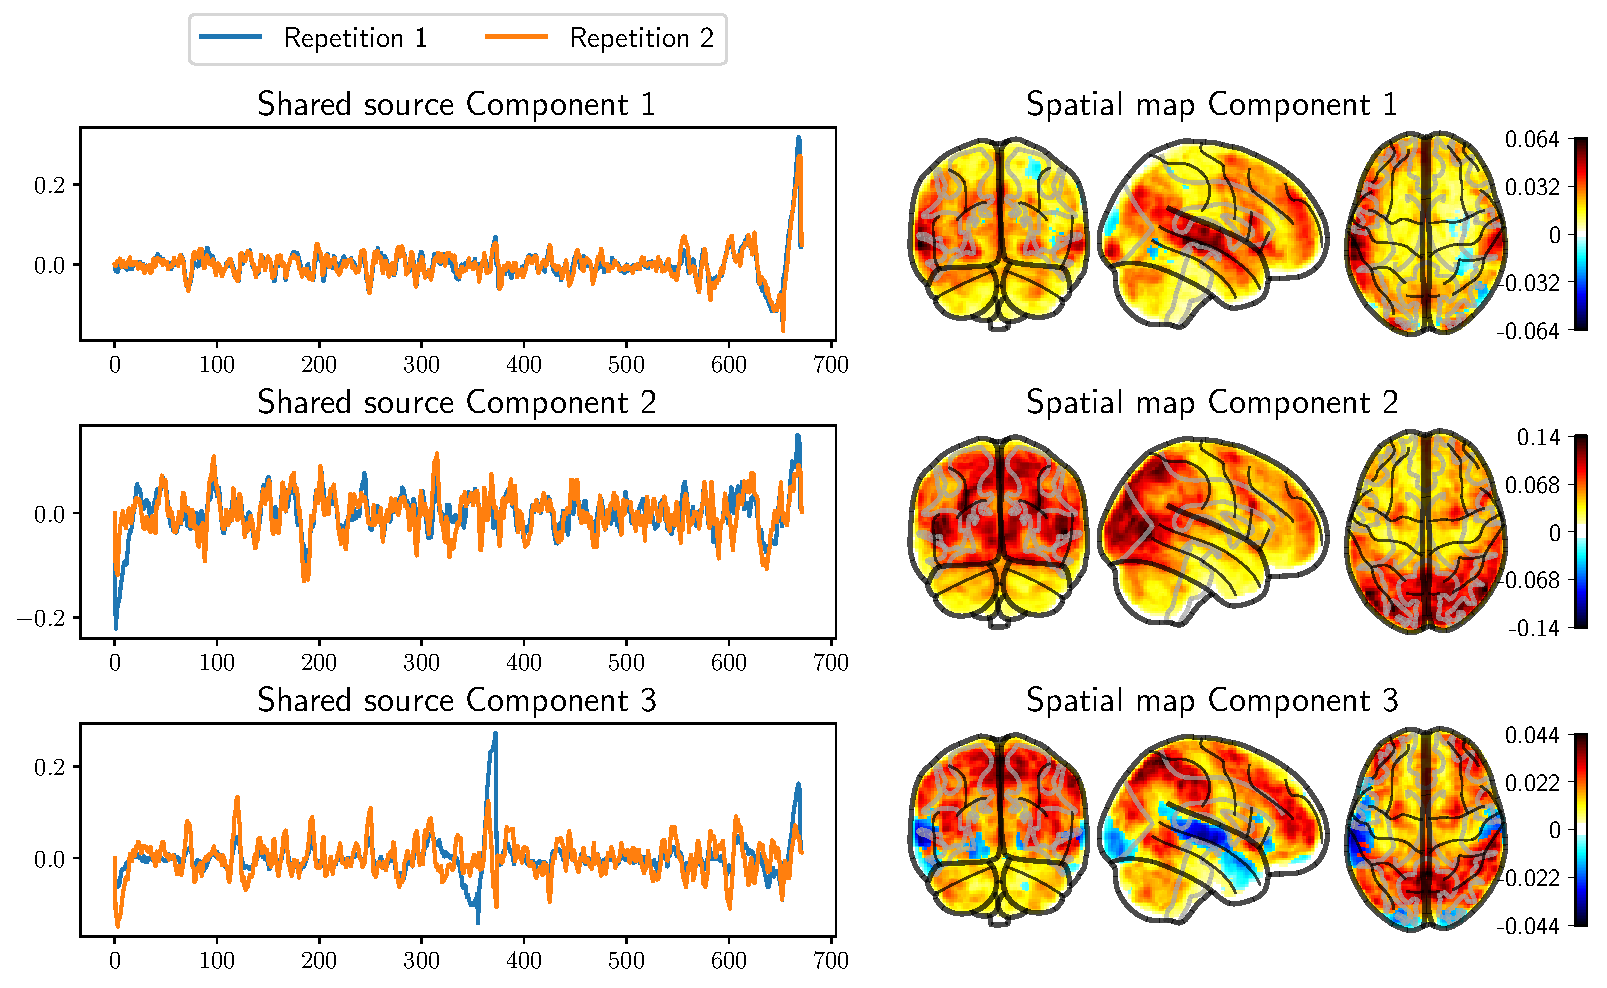
\includegraphics[width=\textwidth]{figures/mvica/swetha_exp_full_fit_appendix.pdf}
  \caption{\textbf{Between-runs time segment matching: spatial maps and timecourses} \emph{Left:} Timecourses of the 3 shared components yielding the highest accuracy. The two displayed set of runs correspond to the same scenes in the movie. \emph{Right:} Localisation of the same shared components in the brain}
  \label{fig:app_spatialmaps}
\end{figure}


%\subsection{MEG experiments}
\section{Phantom MEG data}
\label{sec:mvica:phantom}
We demonstrate the usefulness of our approach on MEG data using the
\emph{Sinusoidal Phantom MEG} dataset where $m=8$ dipoles at different locations
produce a known sinusoidal oscillation (more details in
section~\ref{sec:meg:datasets}). 100 epochs are available.
%
For each dipole, we chose $N_e=2, \dots, 16$ epochs at random among our set of 100 epochs and concatenate them in the temporal dimension.
%
We then apply algorithms on these data to extract $p=20$ shared components.
%
As we know the true component (the timecourse of the dipole), we can compute the reconstruction error of each component as the squared norm of the difference between the estimated component and the true component, after normalization to unit variance and fixing the sign.
%
We only retain the component yielding minimal error.
%
We also estimate for each forward operator the localization of the component by performing dipole fitting using its column corresponding to the component of minimal error.
%
We then compute the distance of the estimated dipole to the true dipole.
%
These metrics are reported in figure~\ref{fig:meg} when the number of epochs considered $N_e$ varies.
%
% We also compare our method to the Bayesian Canonical Correlation Analysis (BCorrCA) of~\cite{kamronn2015multiview}.
% %
% On this task, BCorrCA is outperformed by ICA methods.
%
MultiView ICA requires fewer epochs to correctly reconstruct and localize the true component.
%

\section{Experiment on CamCAN dataset}
Finally, we apply MultiView ICA on the CamCAN
dataset~\cite{taylor2017cambridge}. A detailed description of the CamCAN dataset
is available in section~\ref{sec:meg:datasets}. We use the magnetometer data from the MEG of
$200$ subjects chosen randomly.
%
Each subject is repeatedly presented an audio-visual stimulus. 
%
The MEG signal corresponding to these trials are then time-averaged to isolate the evoked response, yielding individual data.
%
MultiView ICA is then applied to extract $20$ shared components.
%
$9$ components were found to correspond to noise by visual inspection, and the $11$ remaining are displayed in figure~\ref{fig:meg}.
%
We observe that MultiView ICA recovers a very clean sequence of evoked potentials with sharp peaks
for early components and slower responses for late components.
%
In order to visualize their localization, we perform component localization for each subject by solving the inverse problem using sLORETA~\cite{pascual2002standardized}, providing a component estimate for each component.
%
Then, we register each component estimate to a common reference brain.
%
Finally, the component estimates are averaged, and thresholded maps are displayed in figure~\ref{fig:meg}.
%
Individual maps corresponding to each component are displayed in appendix~\ref{sec:app_montages}.
The figure highlights both early auditory and visual cortices, also suggesting a propagation
of the activity towards the ventral regions and higher level visual areas.

\begin{figure}
    \centering

          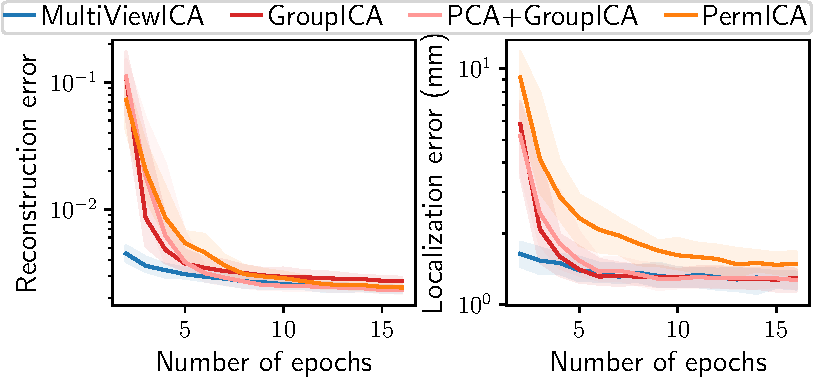
\includegraphics[width=0.6\textwidth]{figures/mvica/phantom.pdf}
          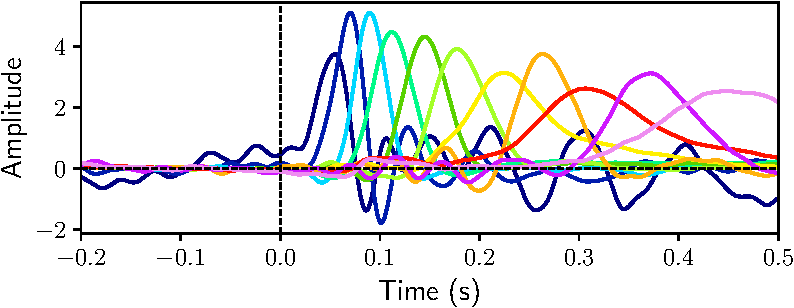
\includegraphics[width=0.6\textwidth]{figures/mvica/camcan_sources.pdf}
          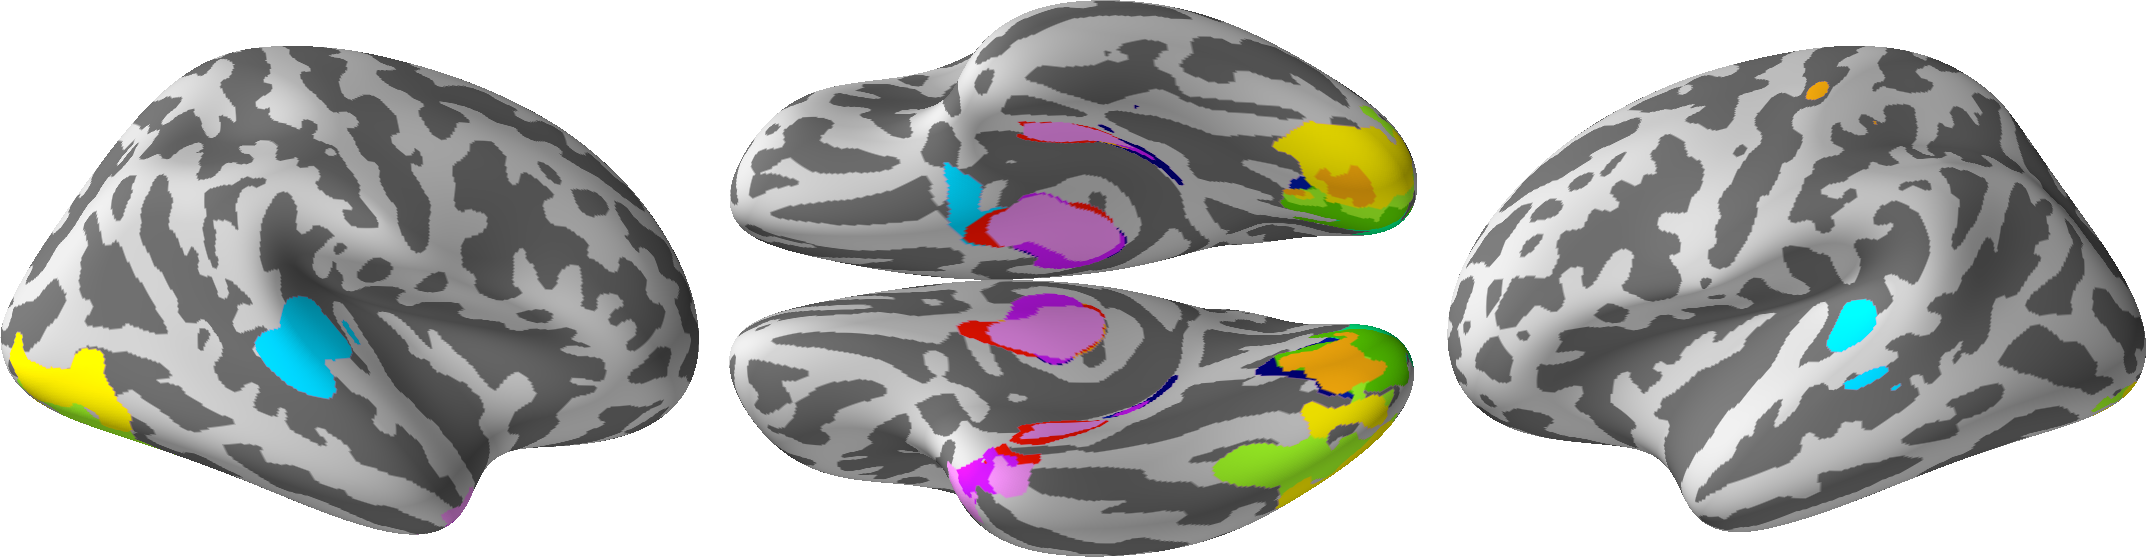
\includegraphics[width=0.6\textwidth]{figures/mvica/montage_all.png}
    \caption{\emph{Top:} \textbf{Experiment on MEG Phantom data}. Reconstruction
      error is the norm of the difference between the estimated and true
      component. Localization error is the distance between the estimated and
      true dipole. \emph{Middle and Bottom:} \textbf{Experiment on 200 subjects from the CAM-can dataset} \emph{Middle:} Time course of $11$ shared components (one color per component). We recover clean evoked potentials. \emph{Bottom:} Associated brain maps, obtained by averaging component estimates registered to a common reference.}
    \label{fig:meg}
\end{figure}

%
%


\section{Conclusion}
In this chapter, we have demonstrated the usefulness of MultiView ICA for neuroimaging group studies both on fMRI and MEG data, where it outperforms other methods.
%
A limiting aspect of MultiView ICA is the assumption that the noise
variance is the same across subjects. This is limiting because it does not
properly model between-subjects variability.
%
In the next chapter, we propose an extension of MultiView ICA with a more realistic
noise model.

% In the experiments on fMRI data, we used temporal ICA in order to make use of the fact that subjects were exposed to the same stimuli. However, applying MultiViewICA on transposed data would carry out spatial ICA. Therefore MultiViewICA can be readily used to analyse different kind of neuroimaging data such as resting state data. 
% %
% Our method is not specific to neuroimaging data and could be relevant to other observational sciences like genomics or astrophysics where ICA is already widely used.
% 
%
%\section{Conclusions}
%\label{sec:conclusions}
%We propose a new method for modeling shared responses in neuroimaging studies. The method is identifiable and, overall, it rocks.
%
%
% \section*{References}
% \section*{Broader Impact}
% We develop a novel unsupervised learning method for Independent Component Analysis of a group of subjects sharing commmon sources.
% %
% Our method is not limited to a particular type of data, and could hence be employed in observational sciences where ICA is relevant: neurosciences, genomics, astrophysics, finance or computer vision for instance.
% %
% ICA is widely used in these fields as a tool among data processing pipelines, and therefore inherits from all the ethical questions of the fields above.
% %
% In particular, data collection bias will result in biased outputs.
% %
% Our algorithm is based on individual linear transforms and therefore decisions based on its application are easier to interpret than more complex models such as deep learning methods: in most applications, the set of parameters has a natural interpretation. For instance in EEG, MEG and fMRI processing, the coefficients of the linear operator can be interpreted as topographic brain maps. 


% \section*{Acknowledgement and funding disclosure}

% This work was supported in part by the French government under management of Agence Nationale de la Recherche as part of the “Investissements d'avenir” program, references ANR19-P3IA-0001 (PRAIRIE 3IA Institute) and ANR17-CONV-0003 (DataIA Institute). It has also received funding from the European Union’s Horizon 2020 Framework Programme for Research and Innovation under the Specific Grant Agreement No. 945539 (Human Brain Project SGA3), the KARAIB AI chair (ANR-20-CHIA-0025-01) and the European Research Council grant ERC-SLAB-StG-676943. L.G. was hosted for part of this project by the Parietal team at Inria, Saclay, while on an ELLIS exchange. A.H. was additionally supported by CIFAR as a Fellow.

\part{Shared ICA}
\label{part:shica}
\chapter{Shared ICA theory}
\label{ch:shica}
In chapter~\ref{ch:mvica1} and chapter~\ref{ch:mvica2}, we have introduced MultiView ICA, a well principled method to perform shared response modeling. 
While MultiView ICA yields good practical results, it does not model subject specific deviations from the shared
response. Yet, the magnitude of the response may differ across subjects \cite{penny2007random}, as does any noise due to heart beats, respiratory artefacts or head movement~\cite{liu2016noise}.
%

This drawback is shared by most GroupICA methods that often rely on single
subject ICA to recover the shared response. In addition, such methods are typically unable to separate Gaussian components.

In contrast, the framework of Independent vector analysis
(IVA)~\cite{lee2008independent, anderson2011joint} allows subject specific
variability in the unmixed data. 
However, current implementations such as IVA-L~\cite{lee2008independent},
IVA-G~\cite{anderson2011joint}, IVA-L-SOS~\cite{bhinge2019extraction}, IVA-GGD~\cite{anderson2014independent} or
IVA with Kotz distribution~\cite{anderson2013independent} only estimate
view-specific components, and do not model or extract a shared response.

% They are thus not well-suited for modelling the dependencies between views in
% functional brain imaging, as we will argue in detail below.

In this chapter, we introduce Shared ICA (ShICA), where each dataset is modeled as a linear transform of shared independent components contaminated by additive Gaussian noise. ShICA allows for principled extraction of the shared components (or responses) in addition to view-specific components. 
%
Since it incorporates a statistically sound noise model, it enables optimal inference (minimum mean squared error, MMSE) of the shared responses.

We first analyse the theoretical properties of the ShICA model, before providing powerful inference algorithms.
First, we exhibit necessary and sufficient conditions for ShICA to be identifiable (previous work only shows local identifiability~\cite{anderson2014independent}), in the presence of Gaussian or non-Gaussian components. 
%
We then introduce an algorithm called ShICA-J that uses Multiset CCA to fit the model when all the components are assumed to be Gaussian. We exhibit necessary and sufficient conditions for Multiset CCA to be able to fit the model (previous work only gives sufficient conditions~\cite{li2009joint}) and provide examples on which ShICA-J can recover the mixing matrices, while Multiset CCA cannot. 
%
We next point out a practical problem, namely that even a small sampling noise can lead to large rotations of unmixing matrices when Multiset CCA is used. To address this issue and recover the correct unmixing matrices, we propose to apply joint diagonalization to the result of Multiset CCA.
%
We further introduce ShICA-ML, a maximum likelihood estimator of ShICA that models non-Gaussian components using a Gaussian mixture model. 
%
While ShICA-ML yields more accurate components, ShICA-J is significantly faster and offers a great initialization to ShICA-ML.

\section{Shared ICA (ShICA): an identifiable multi-view model}
We assume a similar generative model as in MultiViewICA:
\begin{equation}
  \label{eq:model}
   \xb_i = A_i(\sbb + \nb_i)
\end{equation}

Like in MultiView ICA we assume that the shared components are statistically independent $p(\sbb) = \prod_{j=1}^p p(s_j)$, and
that the individual noises are Gaussian and independent from the shared
components. We assume $\nb_i \sim\mathcal{N}(0, \Sigma_i)$, where the matrices
$\Sigma_i$ are assumed diagonal and positive. This contrasts with MultiView ICA: the individual noise variances are learned and are not assumed to be the same across
components or subjects.
We further assume that there are at least 3 views: $m \geq 3$. 

In contrast to almost all existing works, we assume that some components (possibly all of them) may be Gaussian, and denote $\mathcal{G}$ the set of Gaussian components: $\sbb_j \sim \mathcal{N}(0, 1)$ for $j \in \mathcal{G}$. The other components are non-Gaussian: for $j\notin \mathcal{G}$, $\sbb_j$ is non-Gaussian.


\paragraph{Identifiability} The parameters of the model are $\Theta = (A_1, \dots, A_m, \Sigma_1, \dots, \Sigma_m)$. We are interested in the identifiability of this model: given observations $\xb_1,\dots, \xb_m$ generated with parameters $\Theta$, are there some other $\Theta'$ that can generate the same observations?
Let us consider the following assumption that requires that the individual noises for Gaussian components are sufficiently diverse:
%
\begin{assumption}[Noise diversity in Gaussian components]
\label{ass:diversity}
For all $j, j' \in \mathcal{G}, j \neq j'$, the sequences $(\Sigma_{ij})_{i=1 \dots m}$ and $(\Sigma_{ij'})_{i=1 \dots m}$ are different where $\Sigma_{ij}$ is the $j, j$ entry of $\Sigma_i$
\end{assumption}

It is readily seen that there is one trivial set of indeterminacies in the problem: if $P \in \mathbb{R}^{p \times p}$ is a sign and permutation matrix the parameters $(A_1 P, \dots, A_m P, P^{\top}\Sigma_1 P, \dots, P^{\top} \Sigma_m P)$ also generate $\xb_1,\dots, \xb_m$. The following theorem shows that under the above assumption, these are the only indeterminacies of the problem.

\begin{theorem}[Identifiability]
\label{thm:identif}
We suppose Assumption~\ref{ass:diversity}. We let $\Theta'=(A_1', \dots, A_m', \Sigma_1', \dots,\Sigma_m')$ another set of parameters, and assume that they also generate $\xb_1,\dots, \xb_m$. Then, there exists a sign and permutation matrix $P$ such that for all $i$, $A_i'=A_iP$, and $\Sigma_i'= P^{\top} \Sigma_i P$.
\end{theorem}
\label{proof:identif}
\begin{proof}
By hypothesis, the covariances verify $C_{ij} =\bbE[\xb_i\xb_j^\top] = A_i(I_p + \delta_{ij}\Sigma_i)A_j^{\top} = A'_i(I_p + \delta_{ij}\Sigma'_i){A'_j}^{\top}$ for all $i, j$. We let $P_i=A_i^{-1}A_i'$. The previous relationship for $j\neq i$ gives $P_iP_j^{\top} = I_p$. Because there are more than 3 views, there is another integer $k \notin\{i,j\}$, and we have $P_iP_k^{\top}= P_jP_k^{\top}=I_p$. This shows that $P_i = P_j$: all these matrices are equal, and we call $P$ their common value. The previous equation also gives $PP^{\top} = I_p$, so $P$ is orthogonal. 
%
We have that $s + n_i$ and $s' + n_i'$ have independent components and $s + n^i
= P(s' + n_i')$. Lemma~\ref{lemma:ica} in appendix~\ref{app:sec:lemmas} (a direct consequence of classical ICA results~\cite{comon1994independent}, Theorem 10) gives $P=\Pi^{-1} \Omega \Pi'$ where $\Pi$ and $\Pi'$ are sign and permutation matrices such that the first $g$ components of $\Pi(s + n_i)$ and $\Pi'(s' + n_i')$ are Gaussian, and $\Omega$ is a block diagonal matrix given by
\[
\Omega = \begin{bmatrix} \Omega_g & 0 \\ 0 & I_{p - g} \end{bmatrix}
\]
where $\Omega_g$ is orthogonal.
%
We call $A^{(g)}$ the first $g \times g$ block of a matrix $A$ so that $\Omega^{(g)} = \Omega_g$.

Then, considering only the Gaussian components, we can write for $i=j$:  
$(\Pi \Sigma_i)^{(g)} = \Omega_g (\Pi' \Sigma'_i)^{(g)} \Omega_g^{\top}$ for all
$i$. This, combined with Assumption~\ref{ass:diversity}, implies that $\Omega_g$
is a sign and permutation matrix (see Lemma~\ref{lemma:eigdecomp} in appendix~\ref{app:sec:lemmas}) and therefore $P$ is a sign and permutation matrix. Then it follows that $I + \Sigma_i = P(I + \Sigma'_i)P^{\top}$ and therefore $\Sigma_i = P \Sigma'_i P^{\top}$ so $\Sigma'_i = P^{\top} \Sigma_i P$.
\end{proof}

Identifiability in the Gaussian case is a consequence of the identifiability results in~\cite{via2011joint} and in the general case, local identifiability results can be derived from the work of ~\cite{anderson2014independent}. 
%
However local identifiability only shows that for a given set of parameters there exists a neighborhood in which no other set of parameters can generate the same observations~\cite{rothenberg1971identification}. In contrast, the proof of Theorem~\ref{thm:identif} shows global identifiability.

% \pierre{Lacks biblio: this result is not from us per se}
Theorem~\ref{thm:identif} shows that the task of recovering the parameters from
the observations is a well-posed problem, under the sufficient condition of
Assumption~\ref{ass:diversity}.  We also note that
Assumption~\ref{ass:diversity} is necessary for identifiability. For instance,
if $j$ and $j'$ are two Gaussian components such that $\Sigma_{ij} =
\Sigma_{ij'}$ for all $i$, then a global rotation of the components $j, j'$
yields the same covariance matrices. The current work assumes $m \geq 3$. In appendix~\ref{app:identifiability} we give an identifiability result for $m=2$.



\section{Estimation of components with noise diversity via joint-diagonalization}

We now consider the computational problem of efficient parameter inference. This section considers components with noise diversity, while the next section deals with non-Gaussian components.


\subsection{Fitting ShICA via Multiset CCA}
If we assume that the components are all Gaussian, % \aapo{[Aapo: move to section 3.1?]}
the covariance of the observations given by
$C_{ij}=  \bbE[\xb_i\xb_j^\top] = A_i(I_p + \delta_{ij}\Sigma_i)A_j^{\top}\enspace
$ are sufficient statistics and methods using only second order information, like Multiset CCA, are candidates to estimate the parameters of the model.
Consider the
matrix $C \in \bbR^{pm \times pm}$ containing $m \times m$ blocks of size $p
\times p$
such that the block $i,j$ is given by $C_{ij}$. Consider the matrix $D$ identical to $C$ excepts that the non-diagonal blocks are filled with zeros. 
Generalized CCA consists in the following generalized eigenvalue problem:
\begin{equation}
\label{eq:eigv}
    C \ub = \lambda D\ub,\enspace \lambda > 0,\enspace \ub\in\bbR^{pm} \enspace .
\end{equation}
  
Consider the matrix $U = [\ub^1, \dots, \ub^p] \in \mathbb{R}^{mp \times p}$ formed by concatenating the $p$ leading eigenvectors of the previous problem ranked in decreasing eigenvalue order. Then, consider $U$ to be formed of $m$ blocks of size $p \times p$ stacked vertically and define $(W_i)^{\top}$ to be the $i$-th block. These $m$ matrices are the output of Multiset CCA. We also denote $\lambda_1 \geq \dots \geq \lambda_p$ the $p$ leading eigenvalues of the problem.
  %\aapo{[Very difficultto understand! First define the matrix by u's, and then say that you take blocks out of it to define the W.]}

An application of the results of \cite{li2009joint} shows that Multiset CCA recovers the mixing matrices of ShICA under some assumptions.
%
\begin{proposition}[Sufficient condition for solving ShICA via Multiset CCA~\cite{li2009joint}]
Let $r_{ijk} = (1 + \Sigma_{ik})^{-\frac12} (1 + \Sigma_{jk})^{-\frac12}$.
%\bt{Hm. What is $\Sigma_{ik}$ ?}
Assume that $(r_{ijk})_k$ is non-increasing. Assume that the maximum eigenvalue $\nu_k$ of matrix $R^{(k)}$ of general element $(r_{ijk})_{ij}$ is such that  $\nu_k = \lambda_k$ 
%\bt{$\nu_k$ is not defined}
.
Assume that $\lambda_1 \dots \lambda_p$ are distinct.
Then, there exists scale matrices $\Gamma_i$ such that $W_i = 
\Gamma_i A_i^{-1}$ for all $i$.
\end{proposition}
This proposition gives a sufficient condition for solving ShICA with Multiset CCA. It needs a particular structure for the noise covariances as well as specific ordering for the eigenvalues. The next theorem shows that we only need $\lambda_1 \dots \lambda_p$ to be distinct for Multiset CCA to solve ShICA:
\begin{assumption}[Unique eigenvectors]
  \label{ass:uniqueeig}
$\lambda_1 \dots \lambda_p$ are distinct.
\end{assumption}
% \pierre{talk a bit about these assumptions and the eigenvalue distribution}
\begin{theorem}
  \label{th:eig}
  We suppose
  Assumption~\ref{ass:uniqueeig} (only). Then, there exists a permutation matrix $P$ and scale matrices $\Gamma_i$ such that $W_i = P\Gamma_i A_i^{-1}$ for all $i$.
\end{theorem}
\label{proof:eig}
\begin{proof}
  Let us denote $W \in \bbR^{mp \times mp}$ the block diagonal matrix with block $i$ given by
  $(A_i)^{-1}$. We have $C \ub = \lambda D \ub  \iff W C W^\top \zb = \lambda W D W^\top \zb
  $ where $\ub = W^\top \zb$. We call $\zb$ a reduced eigenvector.
  Each
  block in $W C W^\top$ and in $W D W^\top$ is diagonal so any reduced eigenvector $\zb = \begin{bmatrix} \zb_1 \\ \vdots \\ \zb_m \end{bmatrix}$ is
  such that the matrix $Z = [\zb_1 \dots \zb_m]$ has exactly one non-zero line.
  Following Lemma~\ref{lemma:nonzerocoord} in appendix~\ref{app:sec:lemmas}, the first $p$ leading reduced
  eigenvectors $\zb^1, \dots, \zb^p$ all have different first non-zero coordinates.
  Therefore the concatenation of the first $p$ leading reduced eigenvectors is given
  by $[\zb^1, \dots \zb^p] = \begin{bmatrix} \Gamma_1 \\ \vdots \\ \Gamma_m \end{bmatrix} P^{\top}$ where $P^{\top} \in \mathbb{R}^{p \times p}$ is a permutation matrix and $\Gamma_i
  \in \mathbb{R}^{p \times p}$ is a diagonal matrix. Therefore, the first $p$
  eigenvectors are given by $[\ub^1 \dots \ub^p] = \begin{bmatrix} W_1^{\top} \\ \vdots \\ W_m^{\top} \end{bmatrix} = \begin{bmatrix} (A_1^{-1})^{\top} \Gamma_1 P^{\top} \\ \vdots \\ (A_m^{-1})^{\top} \Gamma_m P^{\top} \end{bmatrix}$  and so $W_i = P \Gamma_i A_i^{-1}$
\end{proof}

This theorem means that solving the generalized eigenvalue problem~\eqref{eq:eigv} allows to recover the mixing matrices up to a scaling and permutation: this form of generalized CCA recovers the parameters of the statistical model.
Note that Assumption~\ref{ass:uniqueeig} is also a necessary condition. Indeed, if two eigenvalues are identical, the eigenvalue problem is not uniquely determined.

%\aapo{[Aapo: due to lack of space the rest of this subsection could be moved to suppl material.]}
We have two different Assumptions, \ref{ass:diversity} and \ref{ass:uniqueeig}, the first of which guarantees theoretical identifiability as per Theorem~\ref{thm:identif} and the second guarantees consistent estimation by Multiset CCA as per Theorem~\ref{th:eig}. Next we will discuss their connections, and show some limitations of the Multiset CCA approach. To begin with, we have the following result about the eigenvalues of the problem~\eqref{eq:eigv} and the $\Sigma_{ij}$.
% \pierre{best not to use a pointer to the appendix in the text, just state the following result}
\begin{proposition}
  \label{prop:eigvals_from_noise}
  For $j\leq p$, let $\lambda_j$ the largest solution of $ \sum_{i=1}^m\frac{1}{\lambda_j(1 + \Sigma_{ij}) -\Sigma_{ij}}=1$. Then, $\lambda_1, \dots, \lambda_p$ are the $p$ largest eigenvalues of problem~\eqref{eq:eigv}.
\end{proposition}
It is easy to see that we then have $\lambda_1, \dots, \lambda_p$ greater than $1$, while the remaining eigenvalues are lower than $1$.
From this proposition, two things appear clearly. First, Assumption~\ref{ass:uniqueeig} implies Assumption~\ref{ass:diversity}.
%
Indeed, if the $\lambda_j$'s are distinct, then the sequences $(\Sigma_{ij})_i$ must also be different from the previous proposition.
%
This is expected as from Theorem~\ref{th:eig}, Assumption~\ref{ass:uniqueeig} implies identifiability, which in turn implies Assumption~\ref{ass:diversity}.
% \pierre{I wrote this but this is really pompous}

Prop.~\ref{prop:eigvals_from_noise} also allows us to derive cases where Assumption~\ref{ass:diversity} holds but not Assumption~\ref{ass:uniqueeig}. The following Proposition shows that we can chose parameters of the model so that the model is identifiable but it cannot be solved using Multiset CCA:
\begin{proposition}
\label{counter}
Assume that for two integers $j, j'$, the sequence $(\Sigma_{ij})_i$ is a permutation of $(\Sigma_{ij'})_i$, i.e. that there exists a permutation of $\{1,\dots, p\}$, $\pi$, such that for all $i$, $\Sigma_{ij} = \Sigma_{\pi(i)j'}$.  Then, $\lambda_j = \lambda_{j'}$.
\end{proposition}
In this setting, Assumption~\ref{ass:diversity} holds so ShICA is identifiable, while Assumption~\ref{ass:uniqueeig} does not hold, so Multiset CCA cannot recover the unmixing matrices.




\subsection{Sampling noise and improved estimation by joint diagonalization} \label{sec:samplingnoise}


The consistency theory for Multiset CCA developed above is conducted under the assumption that the
covariances $C_{ij}$ are the true covariances of the model, and not
approximations obtained from observed samples. In practice, however, a serious limitation of Multiset CCA is that even a slight error of estimation on the covariances, due to ``sampling noise'', can yield a large error in the estimation of the unmixing matrices, as will be shown next.


\begin{wrapfigure}{r}{.4\textwidth}
\centering
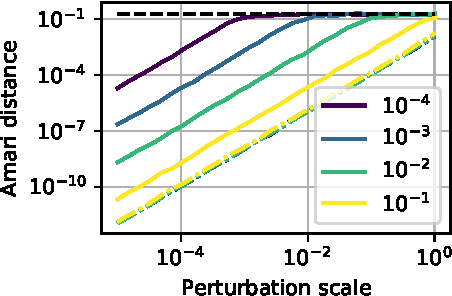
\includegraphics[width=.99\linewidth]{figures/amvica/multicca_gap_jd.pdf}
\caption{Amari distance between true mixing matrices and estimates of Multiset CCA when covariances are perturbed. Different curves correspond to different eigen-gaps. When the gap is small, a small perturbation can lead to complete mixing. Joint-diagonalization (colored dotted lines) fixes the problem.}
\label{fig:cca_gap}
\end{wrapfigure}
We begin with an empirical illustration. We take $m=3$, $p=2$, and $\Sigma_i$ such that $\lambda_1 = 2 + \varepsilon$ and $\lambda_2 =2$ for $\varepsilon > 0$.
%
In this way, we can control the \emph{eigen-gap} of the problem, $\varepsilon$.
%
%
We take $W_i$ the outputs of Multiset CCA applied to the true covariances $C_{ij}$.
%
Then, we generate a perturbation $\Delta = \delta \cdot S$, where $S$ is a random positive symmetric $pm \times pm$ matrix of norm $1$, and $\delta >0$ controls the scale of the perturbation. 
%
We take $\Delta_{ij}$ the $p\times p$ block of $\Delta$ in position $(i, j)$, and $\tilde{W}_i$ the output of Multiset CCA applied to the covariances $C_{ij} + \Delta_{ij}$.
%
We finally compute the sum of the Amari distance between the $W_i$ and $\tilde{W}_i$: the Amari distance measures how close the two matrices are, up to scale and permutation~\cite{amari1996new}.
%\Alex{add ref to paper that explicits the Amari distance}
Fig~\ref{fig:cca_gap} displays the median Amari distance over 100 random repetitions, as the perturbation scale $\delta$ increases. The different curves correspond to different values of the eigen-gap $\varepsilon$. We see clearly that the robustness of Multiset CCA critically depends on the eigen-gap, and when it is small, even a small perturbation of the input (due, for instance, to sampling noise) can lead to large estimation errors.


This problem is very general and well studied~\cite{stewart1973error}: the mapping from matrices to (generalized) eigenvectors is highly non-smooth.
%
However, the gist of our method is that the \emph{span} of the leading $p$ eigenvectors is smooth, as long as there is a large enough gap between  $\lambda_p$ and $\lambda_{p+1}$.
For our specific problem we have the following bounds, derived from Prop.~\ref{prop:eigvals_from_noise}.
\begin{proposition}
  We let $\sigma_{\max} = \max_{ij}\Sigma_{ij}$ and $\sigma_{\min} = \min_{ij}\Sigma_{ij}$. Then, $\lambda_p \geq 1 + \frac{m-1}{1+\sigma_{\max}}$, while $\lambda_{p+1}\leq 1 - \frac{1}{1 + \sigma_{min}}$.
\end{proposition}
As a consequence, we have $\lambda_{p} -\lambda_{p+1} \geq \frac{m-1}{1+\sigma_{\max}} + \frac{1}{1+ \sigma_{\min}}$: the gap between these eigenvalues increases with $m$, and decreases with the noise power.

  \begin{algorithm}[H]
    \SetAlgoLined
  \caption{ShICA-J}
  \label{algo:shicaj}
  \KwIn{Covariances $\tilde{C}_{ij} =
    \bbE[\xb_i\xb_j^{\top}]$}
    $(\tilde{W}_i)_i \leftarrow \mathrm{MultisetCCA}((\tilde{C}_{ij})_{ij})$ \\
        $Q \leftarrow
        \mathrm{JointDiag}((\tilde{W}_i\tilde{C}_{ii}\tilde{W}_i^{\top})_i)$ \\
       $\Gamma_{ij} \leftarrow Q\tilde{W}_i\tilde{C}_{ij}W_j^\top Q^\top$ \\
       $(\Phi_i)_i \leftarrow \mathrm{Scaling}((\Gamma_{ij})_{ij})$ \\
   \Return{Unmixing matrices $(\Phi_iQ\tilde{W}_i)_i$}
  \end{algorithm}

In this setting, when the magnitude of the perturbation $\Delta$ is smaller than $\lambda_{p}-\lambda_{p+1}$, ~\cite{stewart1973error} indicates that $\mathrm{Span}([W_1, \dots, W_m]^{\top})\simeq \mathrm{Span}([\tilde{W}_1,\dots, \tilde{W}_m]^\top)$, where $[W_1, \dots, W_m]^{\top}\in\bbR^{pm\times p}$ is the vertical concatenation of the $W_i$'s.
In turn, this shows that there exists a matrix $Q\in\bbR^{p\times p}$ such that
%
%
\begin{equation}
    \label{eq:justif_jd}
    W_i \simeq Q\tilde{W}_i\enspace \text{for all} \enspace i.
\end{equation}

We propose to use joint-diagonalization to recover the matrix $Q$. Given the $\tilde{W}_i$'s, we consider the set of symmetric matrices $\tilde{K}_i = \tilde{W}_i\tilde{C}_{ii}\tilde{W}_i^{\top}$, where $\tilde{C}_{ii}$ is the contaminated covariance of $\xb_i$. Following Eq.~\eqref{eq:justif_jd}, we have $Q\tilde{K}_iQ^{\top} = W_i \tilde{C}_{ii}W_i^{\top}$, and using Theorem~\ref{th:eig}, we have $Q\tilde{K}_iQ^{\top} = P\Gamma_i A_i^{-1}\tilde{C}_{ii}A_i^{-\top}\Gamma_iP^{\top}$. Since $\tilde{C}_{ii}$ is close to $C_{ii} = A_i (I_p + \Sigma_i)A_i^\top$, the matrix $P\Gamma_i A_i^{-1}\tilde{C}_{ii}A_i^{-\top}\Gamma_iP^{\top}$ is almost diagonal.
%
In other words, the matrix $Q$ is an approximate diagonalizer of the $\tilde{K}_i$'s, and we approximate $Q$ by joint-diagonalization of the $\tilde{K}_i$'s. In Fig~\ref{fig:cca_gap}, we see that this procedure mitigates the problems of multiset-CCA, and gets uniformly better performance regardless of the eigen-gap.
%
In practice, we use a fast joint-diagonalization
algorithm~\cite{ablin2018beyond} to minimize a joint-diagonalization criterion
for positive symmetric matrices~\cite{pham2001joint}. The estimated unmixing
matrices
\begin{align}
U_i = Q\tilde{W}_i
\end{align}
correspond to the true unmixing matrices only up to some scaling: the information that the components are of unit variance is lost.

\textbf{Scale estimation}
We form the matrices $\Gamma_{ij} = U_i\tilde{C}_{ij}U_j^\top$. In order to
estimate the scalings, we solve
\begin{align}
\loss_{\Phi} = \min_{(\Phi_i)} \sum_{i\neq j} \| \Phi_i \diag(\Gamma_{ij}) \Phi_j - I_p \|_F^2
\end{align}
where the $\Phi_i$ are diagonal matrices.
The gradient is given by
\begin{align}
  \partialfrac{\Phi_i}{\loss_{\Phi}} = 2\sum_{j \neq i} (\Phi_i \diag(Y_{ij}) \Phi_j - I_p) \Phi_j
\end{align}
Therefore we get
\begin{align}
  &\partialfrac{\Phi_i}{\loss_{\Phi}} = 0 \\
  &\iff 2\sum_{j \neq i} (\Phi_i \diag(Y_{ij}) \Phi_j - I_p) \Phi_j = 0 \\
  &\iff \Phi_i \sum_{j \neq i} \diag(Y_{ij}) \Phi_j^2 - \sum_{j \neq i} \Phi_j = 0 \\
  &\iff \Phi_i = \frac{\sum_{j \neq i} \Phi_j}{\sum_{j \neq i} \diag(Y_{ij}) \Phi_j^2}
    \label{eq:phiupdates}
\end{align}
We then iterate formula~\eqref{eq:phiupdates} over $i$ until convergence.
The final estimates of the unmixing matrices are given by
\begin{align}
  (\Phi_i U_i)_{i=1}^m
\end{align}
The full procedure, called ShICA-J, is summarized in Algorithm~\ref{algo:shicaj}.

\subsection{Estimation of noise covariance and inference of shared components}

In practice, it is important to estimate noise co-variances $\Sigma_i$ in order to take advantage of the fact that some views are noisier than others. As it is well known in classical factor analysis, modelling noise variances allows the model to virtually discard variables, or subjects, that are particularly noisy. 

Using the ShICA model with Gaussian components, we derive noise covariances estimate directly from maximum likelihood. We use an expectation-maximization (EM) algorithm, which is especially fast because noise updates are in closed-form. Following derivations given in appendix~\ref{conditional_density}, the sufficient statistics in the E-step are given by 
\begin{align}
\label{mmse1}
&\EE[\sbb|\xb]= \left(\sum_{i=1}^m \Sigma_i^{-1}  + I \right)^{-1}  \sum_{i=1}^m \left(\Sigma_i^{-1} \yb_i \right) \\
     &\VV[\sbb|\xb]= (\sum_{i=1}^m \Sigma_i^{-1}  + I)^{-1}
\end{align}
Incorporating the M-step we get the following updates that only depend on the covariance matrices:
\begin{align*}
  \Sigma_i \leftarrow &\diag(\hat{C_{ii}} - 2 \VV[\sbb | \xb]  \sum_{j=1}^m \Sigma_j^{-1} \hat{C}_{ji} \\&  + \VV[\sbb | \xb]  \sum_{j = 1}^m \sum_{l = 1}^m \left(\Sigma_j^{-1} \hat{C}_{jl} \Sigma_l^{-1} \right) \VV[\sbb | \xb] + \VV[\sbb | \xb])
  \numberthis
\end{align*}
%We observe very fast convergence ($10$ iterations are usually enough to reach gradients $\ell_2$ norm below $10^{-4}$).

\section{ShICA-ML: Maximum likelihood for non-Gaussian components}
ShICA-J only uses second order statistics. However, the ShICA model~\eqref{eq:model} allows for non-Gaussian components. We now propose an algorithm for fitting the ShICA model that assumes non-Gaussian components so that it can separate Gaussian and non-Gaussian components.
%\aapo{[Aapo: Motivate and link to previous sections]}
We estimate the parameters by maximum likelihood. Since most non-Gaussian
components in real data are super-Gaussian, we assume that the non-Gaussian
components $\sbb$ have the super-Gaussian density
\begin{equation}
  p(s_j) = \frac12\left(\mathcal{N}( s_j; 0, \frac12) + \mathcal{N}( s_j; 0, \frac{3}{2})\right)
\end{equation}

We propose to maximize the log-likelihood using a generalized
EM~\cite{neal1998view, dempster1977maximum}. Derivations are available in Appendix~\ref{app:emestep}. Like in the previous section, the E-step is in closed-form yielding the following sufficient statistics:
  \begin{align}
    \label{mmse2}
    &\EE[s_j | \xb] = \frac{\sum_{\alpha \in \{\frac12, \frac32\}} \theta_{\alpha} \frac{\alpha \bar{y}_{j}}{\alpha + \bar{\Sigma_{j}}}}{\sum_{\alpha \in \{0.5, 1.5\}} \theta_{\alpha}} \\
    & \VV[s_j | \xb] = \frac{\sum_{\alpha \in \{\frac12, \frac32\}} \theta_{\alpha} \frac{\bar{\Sigma_{j}}\alpha}{\alpha + \bar{\Sigma_{j}}}}{\sum_{\alpha \in \{0.5, 1.5\}} \theta_{\alpha}}  
\end{align}
where $\theta_{\alpha} = \Ncal(\bar{y}_{j}; 0 , \bar{\Sigma}_{j} + \alpha)$, 
$\bar{y}_j = \frac{\sum_i \Sigma_{ij}^{-1} y_{ij}}{ \sum_i
  \Sigma_{ij}^{-1}}$ and $\bar{\Sigma_{j}} = (\sum_i
\Sigma_{ij}^{-1})^{-1}$ with $\yb_i = W_i \xb_i$.
Noise updates are in closed-form and given by:
\begin{align}
\Sigma_i \leftarrow  \diag((\yb_i - \EE[\sbb | \xb]) (\yb_i - \EE[\sbb | \xb])^{\top}+ \VV[\sbb | \xb])
\end{align}
However, no closed-form is available for the updates of unmixing matrices. We therefore perform quasi-Newton updates given by
\begin{align}
  W_i \leftarrow (I - \rho (\widehat{\mathcal{H}^{W_i}})^{-1} \mathcal{G}^{W_i}) W_i
\end{align}
where $\rho \in \mathbb{R}$ is chosen by backtracking line-search

\begin{align}
	\widehat{\mathcal{H}^{W_i}_{a, b, c, d}} =  \delta_{ad} \delta_{bc} + \delta_{ac} \delta_{bd}\frac{(y_{ib})^2}{\Sigma_{ia}}
\end{align}
is an approximation of the Hessian of the negative complete log-likelihood and
\begin{align}
	\mathcal{G}^{W_i} = -I + (\Sigma_i)^{-1}(\yb_i - \mathbb{E}[\sbb|\xb])(\yb_i)^{\top}
\end{align}
 is the gradient.

We alternate between computing the statistics $\mathbb{E}[\sbb|\xb]$, 
$\mathbb{V}[\sbb|\xb]$ (E-step) and updates of parameters $\Sigma_i$ and $W_i$ for $i=1 \dots m$ (M-step). Let us highlight that our EM algorithm and in particular the E-step resembles the one used in~\cite{moulines1997maximum}. However because they assume noise on the sensors and not on the components, their formula for $\EE[\sbb| \xb]$ involves a sum with $2^p$ terms whereas we have only $2$ terms. The resulting method is called ShICA-ML.

\paragraph{Minimum mean squared error estimates in ShICA}
In ShICA-J as well as in ShICA-ML, we have a closed-form for the expected components given the data $\EE[\sbb | \xb]$, shown in equation~\eqref{mmse1} and~\eqref{mmse2} respectively. This provides minimum mean squared error estimates of the shared components, and is an important benefit of explicitly modelling shared components in a probabilistic framework.
\section{Related Work}
ShICA combines theory and methods coming from different branches of ``component analysis''. It can be viewed as a GroupICA method, as an extension of Multiset CCA, as an Independent Vector Analysis method or, crucially, as an extension of SRM. In the setting studied here, ShICA improves upon all existing methods.

ShICA inherits from all the advantages of MultiView ICA. Unlike CanICA or ConcatICA
(see section~\ref{sec:canicaandconcatica}), it optimizes a
proper likelihood and unlike tensorial
methods~\cite{beckmann2005tensorial} or SRM, it does not assume any structure on
the mixing matrices.

Compared to the likelihood based method of Guo presented in section~\ref{sec:guo} or to MultiView ICA, ShICA allows different subjects to have different noise
variances. This last point is crucial as it allows to separate Gaussian components. In addition, the estimation in ShICA-ML relies on a very efficient closed form
E-step. This differs from the likelihood based method of Guo that does not have
a closed form E-step and has to rely on a first order approximation.

ShICA-J uses the Multiset CCA presented in section~\ref{sec:mcca} which is one of the fastest as it reduces to solving a generalized eigenvalue problem. The fact that CCA solves a well defined probabilistic model has first been studied in~\cite{bach2005probabilistic} where it is shown that CCA is identical to multiple battery factor analysis~\cite{browne1980factor} (restricted to 2 views). This latter formulation differs from our model in that the noise is added on the sensors and not on the components which makes the model unidentifiable. Identifiable variants and
generalizations can be obtained by imposing sparsity on the mixing matrices such as in~\cite{archambeau2008sparse, klami2014group, witten2009extensions} or non-negativity~\cite{DELEUS2011143}.
Lastly, the work in~\cite{li2009joint} exhibits a set of sufficient (but not necessary) conditions under which a well defined model can be learnt by the formulation of Multiset CCA used in ShICA-J. The set of conditions we exhibit in this work are necessary and sufficient. We further emphasize that basic Multiset CCA provides a poor estimator, as explained in section~\ref{sec:samplingnoise}.

Let us highlight that ShICA can be seen as a particular instance of IVA where
subject specific components $s_{ij}$ are such that $s_{ij} = s_j + n_{ij}$.
However, current implementations such as IVA-L~\cite{lee2008independent},
IVA-G~\cite{anderson2011joint}, IVA-L-SOS~\cite{bhinge2019extraction}, IVA-GGD~\cite{anderson2014independent} or
IVA with Kotz distribution~\cite{anderson2013independent} only estimate
view-specific components, and do not model or extract a shared response.
In contrast, ShICA specifically enables extraction of shared components from the
subject specific components via its minimum mean squared error estimate.

The IVA theory provides global identifiability conditions in the Gaussian case (IVA-G)~\cite{via2011joint} and local identifiability conditions in the general case~\cite{anderson2014independent} from which local identifiability conditions of ShICA could be derived. However, in this work, we provide global identifiability conditions for ShICA.
Lastly, IVA can be performed using joint diagonalization of cross covariances~\cite{li2011joint, congedo2012orthogonal} although multiple matrices have to be learnt and cross-covariances are not necessarily symmetric positive definite, which makes the algorithm slower and less principled.

Let us point out that extracting a shared response from multiple dataset is also
the goal of SRM. Some deep variants~\cite{chen2016convolutional} release the
orthogonality constrain but they are much more computationally demanding.
ShICA leverages ICA theory to provide a much more powerful model of shared responses.

\paragraph{Limitations}
[Omitted long matching line]

\section{Conclusion}
[Omitted long matching line]
In the next chapter, we evaluate ShICA using both real and synthetic data and
compare with competitive approaches.

\chapter{Shared ICA in practice}
\label{ch:shica2}
In the previous chapter, we have introduced the ShICA model, a principled
unifying solution to the problems of shared response
modeling and GroupICA. In this chapter we evaluate its practical utility on
synthetic data and on brain imaging data.

\section{Synthetic experiment}
In the following synthetic experiments, data are generated according to model~\eqref{eq:model} with $p=4$ components and $m=5$ views and mixing matrices are generated by sampling coefficients from a standardized Gaussian.
\subsection{Separation performance: different use cases}
\label{sec:rotation}
%\pierre{Make sure that algos are always in the same order in legend, and that shica-j and shica ml are together}
Gaussian components are generated from a standardized Gaussian and their noise
has standard deviation $\Sigma_i^{\frac12}$ where $\Sigma_i^{\frac12}$ is a
[Omitted long matching line]
\begin{figure}
\centering
  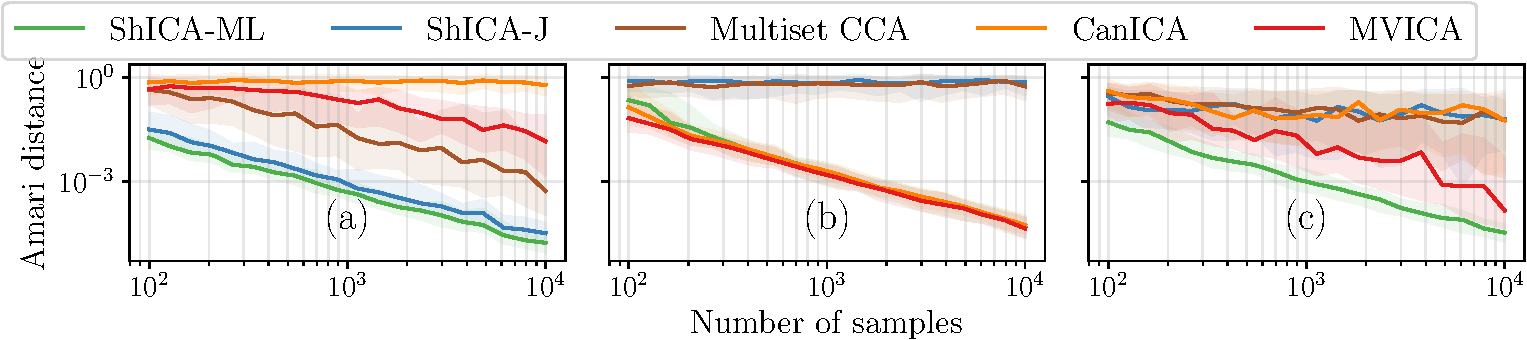
\includegraphics[width=0.9\textwidth]{./figures/amvica/identifiability.pdf}
  \caption{\textbf{Separation performance}: Algorithms are fit on data following model~\ref{eq:model} \textbf{(a)} Gaussian components with noise diversity \textbf{(b)} Non-Gaussian components without noise diversity \textbf{(c)} Half of the components are Gaussian with noise diversity, the other half is non-Gaussian without noise diversity. 
  %\aapo{[It would be nice to have labels a,b,c but this is not critical.]}
  %\Alex{Make the legend fit on one line and rename Multiset CCA to Multiset CCA to be consistent with the text (or update text). Also you should be able to reduce a tiny bit the height of the axes plots.}
  }
  \label{exp:rotation}
\end{figure}
When all components are Gaussian (Fig.~\ref{exp:rotation}~(a)), CanICA cannot
separate the components at all. In contrast ShICA-J, ShICA-ML and Multiset CCA
are able to separate them, but Multiset CCA needs many more samples to reach the
same Amari distance as ShICA-J or ShICA-ML, which shows that correcting for the
rotation due to sampling noise improves the results. Looking at error bars, we
also see that the performance of Multiset CCA varies quite a lot with the random
seeds: this shows that depending on the sampling noise, the rotation can be very
different from identity. MultiViewICA does achieve separation but obtains
relatively poor separation performance compared to ShICA or Multiset CCA.
When none of the components are Gaussian (Fig.~\ref{exp:rotation}~(b)), only
CanICA, ShICA-ML and MultiView ICA are able to separate the components, as other methods do not make use of non-Gaussianity.
Finally, in the hybrid case (Fig.~\ref{exp:rotation}~(c)), ShICA-ML is able to
separate the components very well as it can make use of both non-Gaussianity and
noise diversity. As we can see, MultiView ICA yields decent performance though
uniformly worse than ShICA-ML. Also note that error bars are very large showing
that for some seeds it gives poor results. Overall, MultiView ICA is a lot less
reliable than ShICA-ML.


\subsection{Separation performance in function of non-Gaussianity}
We generate data according to model~\eqref{eq:model}. Components $\sbb$ are
generated using $s_j = d(x)$ with $d(x) = x |x|^{\alpha - 1}$ and $x \sim
\mathcal{N}(0, 1)$. We impose noise diversity: the noise of view $i$ has standard deviation $\Sigma_i^{\frac12}$ (obtained by sampling from a uniform density between $0$ and $1$).
[Omitted long matching line]
 When $\alpha$ is close to 1 (components are almost Gaussian), ShICA-J, ShICA-ML and multiset CCA can separate components well (but multiset CCA reaches higher Amari distance than ShICA). In this regime, MultiViewICA yields much higher Amari distance than ShICA-J, ShICA-ML or Multiset CCA but is still better than CanICA which cannot separate components at all.
 As non-Gaussianity ($\alpha$) increases, ICA based methods yield better results but ShICA-ML yields uniformly lower Amari distance.
\begin{figure}
\centering
  \includegraphics[width=0.8\textwidth]{./figures/amvica/synthetic_Gaussian_source.pdf}
  \caption{\textbf{ Separation performance in function of non-Gaussianity} Separation performance of algorithms for sub-Gaussian $\alpha < 1$ and super-Gaussian $\alpha > 1$ components}
  \label{exp:separatingpower}
\end{figure}

\subsection{Computation time}
\begin{figure}
    \centering
    \includegraphics[width=.65\linewidth]{./figures/amvica/synthetic_Gaussian_timings.pdf}
    \caption{\textbf{Computation time: } Algorithms are fit on data generated from model~\eqref{eq:model} with a super-Gaussian density. For different values of the number of samples, we plot the Amari distance and the fitting time. Thick lines link median values across seeds.}
    \label{exp:syn_timings}
\end{figure}
[Omitted long matching line]
%


%\pierre{fig might have a smaller legend: 3 cols, smaller fonts}


% The difference between AVICA and other approaches can be quantified via a
% statistical t-test on the difference of log distances. It
% gives the p-values $4.57 \times 10^{-4}$, $5.93 \times 10^{-4}$ and $2.37
% \times 10^{-9}$ w.r.t.
% MVICA, PermICA and ConcatICA respectively.
\section{Experiments on brain imaging data}

\subsection{Robustness w.r.t intra-subject variability in MEG}
\begin{figure}
  \centering
  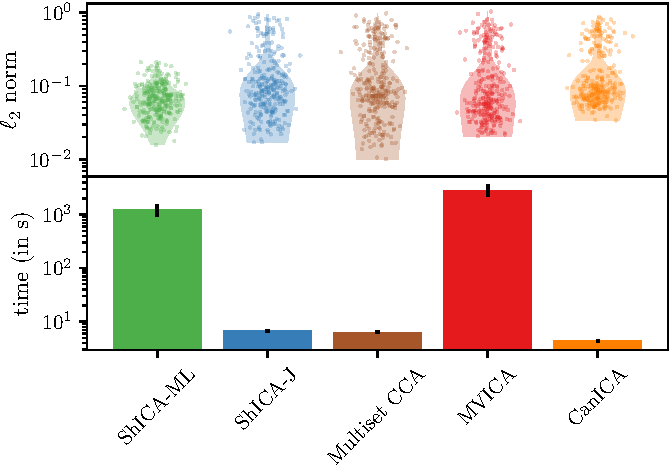
\includegraphics[width=.65\linewidth]{./figures/amvica/inter_subject_stability.pdf}
  \caption{\textbf{Robustness w.r.t intra-subject variability in MEG}:
    (\textbf{top}) $\ell_2$ distance between shared components corresponding to the same stimuli in different trials.  (\textbf{bottom}) Fitting time.
    %\Alex{Should be $\ell_2$ in ylabel not L2}
}
\label{fig:eeg_intragroup_variability}
\end{figure}
In the following experiments we consider the Cam-CAN
dataset~\cite{taylor2017cambridge}. We use the magnetometer data from the MEG of $m=100$ subjects chosen randomly among 496.
% 
Each subject is repeatedly presented three audio-visual stimuli. 
% 
For each stimulus, we divide the trials into two sets and within each set, %Aapo: "sets"
the MEG signal is averaged across trials to isolate the evoked response. This
procedure yields 6 chunks of individual data (2 per stimulus).
%
% The 6 chunks of data are concatenated in the time direction and ICA algorithms
% are applied separately to extract $k=10$ shared components that we plot in
% appendix~\ref{megcomponents} and localize in appendix~\ref{megcomponentslocal}.
%
We study the similarity between shared components corresponding to repetitions of the same stimulus. This gives a measure of robustness of each ICA algorithm with respect
to intra-subject variability.
Data are first reduced using a subject-specific PCA with $p=10$ components. Algorithms are run 10 times with different seeds on the 6 chunks of data,
and shared components are extracted.
%
When two chunks of data correspond to repetitions of the same stimulus they should yield similar
components.
%
For each component and for each stimulus, we therefore measure the $\ell_2$
distance between the two repetitions of the stimulus.
 This yields $300$ distances per algorithm that are
plotted on Fig~\ref{fig:eeg_intragroup_variability}.

The components recovered by ShICA-ML have a much lower variability than other approaches. The performance of ShICA-J is competitive with Multiview ICA while being much faster to fit. Multiset CCA yields satisfying results compared with ShICA-J. However we see that the number of components that do not match at all across trials is greater in Multiset CCA.

The mixing operators in ShICA define spatial maps. In appendix~\ref{app:shica:maps}, we plot
the average spatial maps across subjects.

    %\bt{Muliview ICA appears only now ?} \aapo{[Actually, multiset CCA looks just as good as ShICA-J?, comments?.]}

\subsection{MEG Phantom experiment}
\label{app:phantom}
\subsubsection{Elekta Phantom}
We use the \emph{Elektra Phantom MEG} dataset described
in~\ref{sec:meg:datasets} where dipoles at $m=32$ different locations emit the
same signal.
    We reduce the data by applying view specific PCA with $k=20$ components and algorithms are applied on the reduced data. We select the component that is closer to the true one and compute the L2 norm between the predicted component and the true one after normalization.
    Then we attempt to recover the position of each dipole by performing dipole fitting on the mixing operator of each view (using only the column corresponding to the true component). The localization error is defined as the mean l2 distance between the true localization and the predicted localization where the mean is computed across dipoles. 
    Each epoch corresponds to 301 samples and 20 epochs are available in total. We vary the number of epochs between 2 and 18 and display in Fig~\ref{exp:meg_phantom} the reconstruction error and the localization error as a function of the number of epochs used.
    ShICA-ML outperforms other methods. ShICA-J gives satisfying results while being much faster.
    
    \subsubsection{MEG Phantom Sinusoidal components}
    We reproduce the phantom experiment presented in section~\ref{sec:mvica:phantom}. ShICA-ML outperforms other methods. ShICA-J gives satisfying results while being much faster.
    
\begin{figure}
\centering
  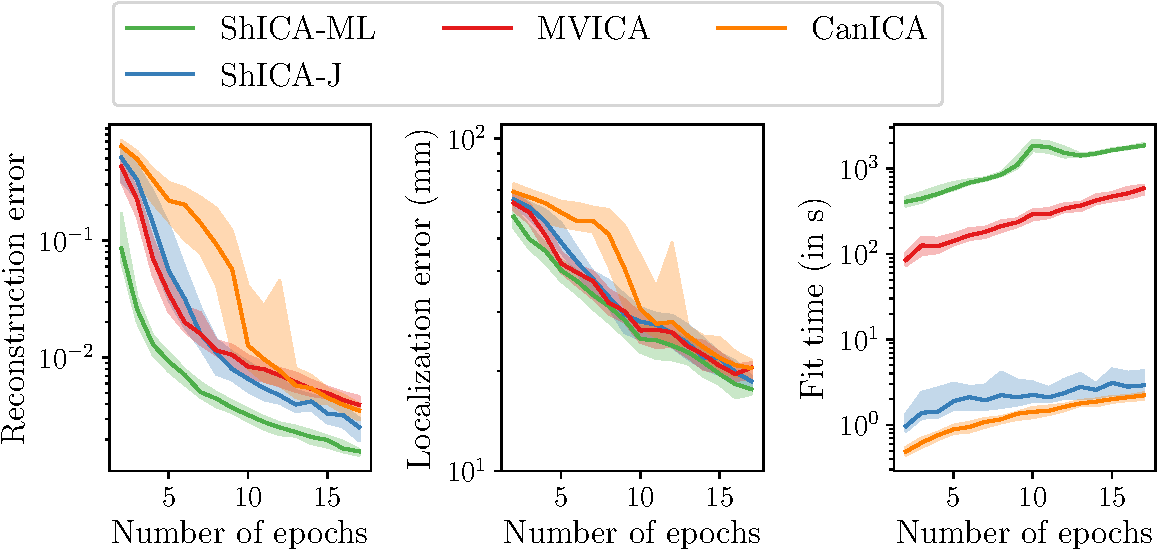
\includegraphics[width=0.9\textwidth]{./figures/amvica/meg_phantom.pdf}
  \caption{\textbf{MEG Phantom (Elekta)}: (left) L2 distance between the predicted and actual component (middle) Mean error (in mm) between predicted and actual dipoles localization (right) Fitting time (in seconds)}
\label{exp:meg_phantom}
\end{figure}

\begin{figure}
\centering
  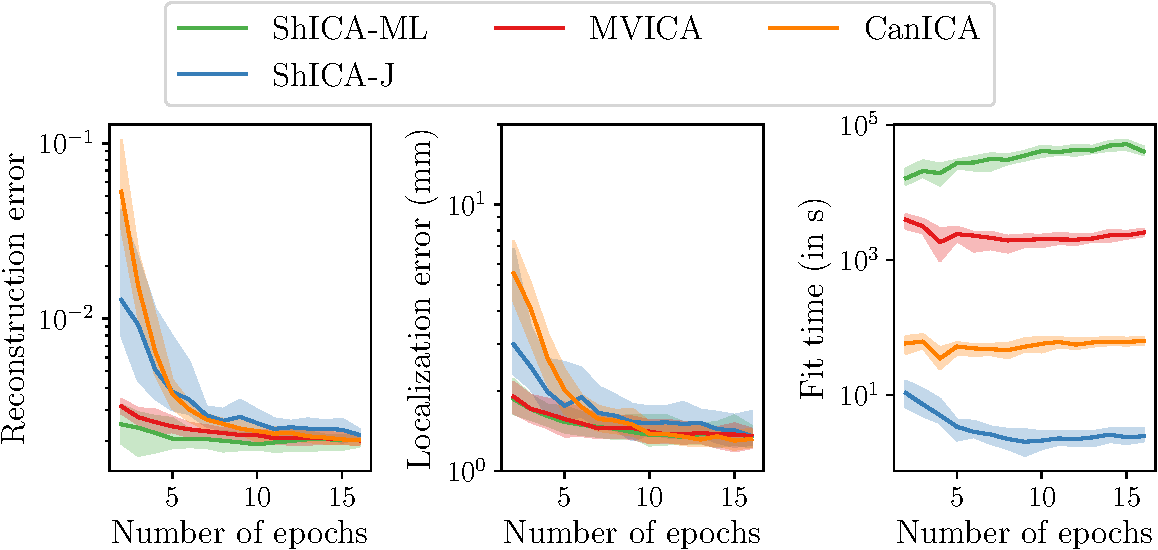
\includegraphics[width=0.9\textwidth]{./figures/amvica/meg_phantom_neurips.pdf}
  \caption{\textbf{MEG Phantom Sinusoidal components}: (left) L2 distance between the predicted and actual component (middle) Mean error (in mm) between predicted and actual dipoles localization (right) Fitting time (in seconds)}
\label{exp:meg_phantom_neurips}
\end{figure}



\subsection{Reconstructing the BOLD signal of missing subjects}
\begin{figure}
  \centering
  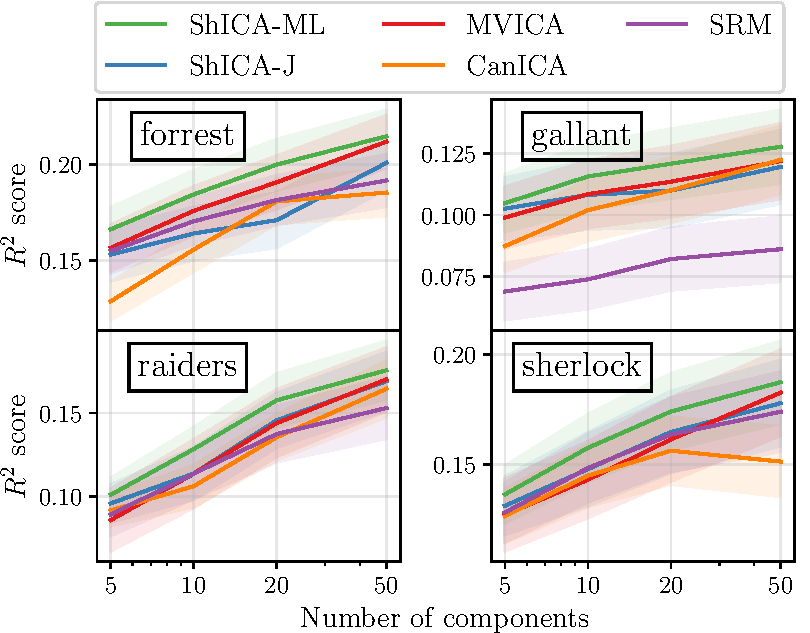
\includegraphics[width=0.49\linewidth]{./figures/amvica/reconstruction.pdf}
  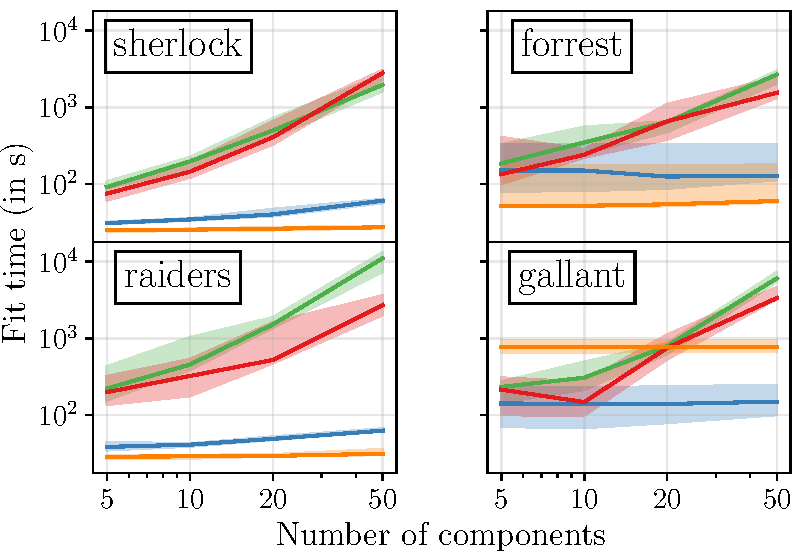
\includegraphics[width=0.49\linewidth]{./figures/amvica/reconstruction_timings.pdf}
  
  \caption{\textbf{Reconstructing the BOLD signal of
      missing subjects}. (\textbf{left}) Mean $R^2$ score between reconstructed data and true
    data. (\textbf{right}) Fitting time.
    %\Alex{ylabel should be $R^2$ not R2}
    }
  \label{fig:reconstruction}
\end{figure}

We reproduce the experiental pipeline described in section~\ref{sec:srm:reconstruction}.
ShICA-ML yields the best $R^2$ score in all datasets and for any number of
components. ShICA-J yields competitive results with respect to Multiview ICA
while being much faster to fit.


\subsection{fMRI timesegment matching experiment}
A popular benchmark especially in the SRM community is the time-segment matching
experiment~\cite{chen2015reduced} which we describe in
section~\ref{timesegment_expe}.
The left panel in Fig~\ref{exp:timesegment} shows that ShICA-ML, MultiViewICA and ShICA-J yield almost equal accuracy and outperform other methods by a large margin. The right panel in Fig~\ref{exp:timesegment} shows that ShICA-J is much faster to fit than MultiViewICA or ShICA-ML.


\begin{figure}
    \centering
    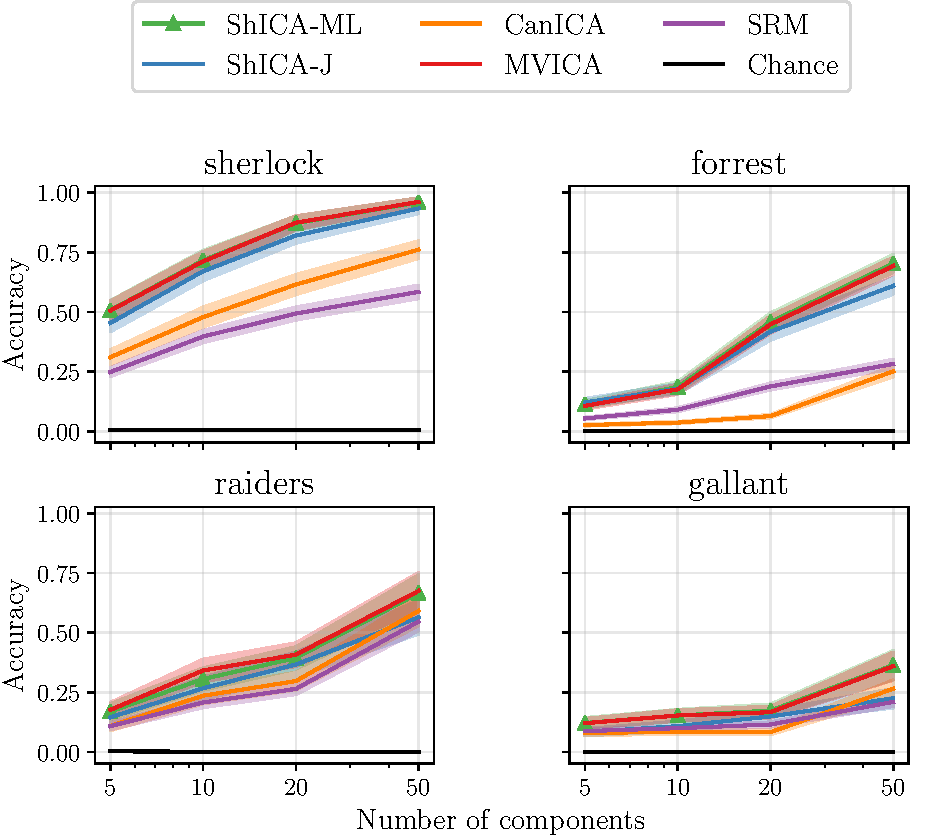
\includegraphics[width=0.49\textwidth]{./figures/amvica/timesegment_matching.pdf}
    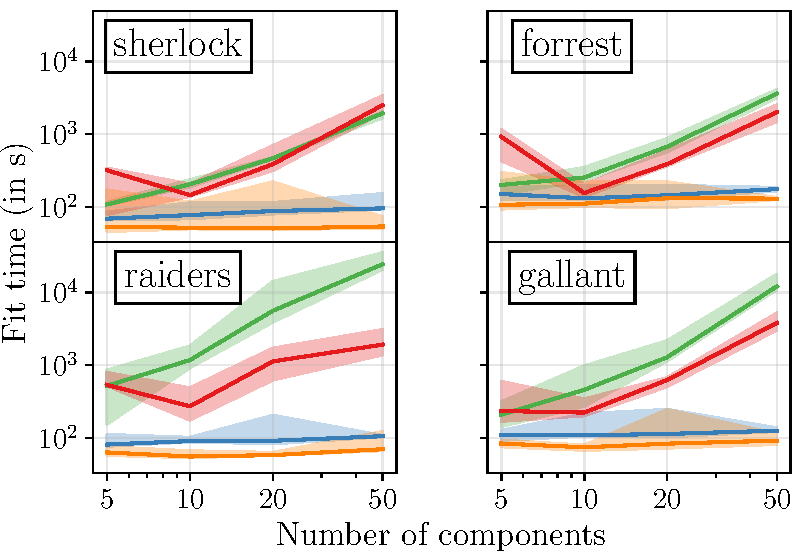
\includegraphics[width=0.49\textwidth]{./figures/amvica/timesegment_matching_timings.pdf}
    \caption{\textbf{Timesegment matching experiment}: (left) Accuracy (right) Fitting time (in seconds)}
    \label{exp:timesegment}
\end{figure}

% AVICA exhibits a small improvement on sherlock and raiders datasets that is
% consistent for different numbers of components (i.e. numbers of components) and competitive results on clips and forrest datasets.

% 

%\pierre{right plot is hard to read, too wide. Lots of space to gain here}

\section{Conclusion}
In this chapter, we have shown the practical benefits of ShICA.
On simulated data, ShICA clearly outperforms all competing methods in terms of the trade-off between statistical accuracy and computation time. On brain imaging data, ShICA gives more stable decompositions for comparable computation times, and more accurately predicts the data of one subject from the data of other subjects, making it a good candidate to perform transfer learning.
%ShICA inherits the ethical questions linked to its field of application.
As ShiCA only involves linear transforms, decisions based on its output are easier to interpret, making it accessible to practitioners.
%This work can help in brain disease diagnosis and reduce their human and societal burden.

In the next section, we show that ICA can be used to perform data augmentation
in fMRI.

% \section{A fast two-step approach for MIFA}

% While maximum-likelihood approaches possess several important statistical properties that make them attractive, a major drawback is the slowness of the algorithms. 
% %
% These method also require the likelihood to be well defined, and prevents dimension reduction without a more complicated model: for the likelihood to be well defined, we must assume that $A_i$ is square, invertible.
% Instead, we propose a two steps ad-hoc method, based on the following observations that were used for proving identifiability:
% \begin{itemize}
%     \item The knowledge of the empirical covariances $C_{ij}$ for $i\neq j$ allows to recover the mixing matrices $A_i$ up to a global rotation matrix.
%     \item Then, the knowledge of the ``diagonal'' terms $C_{ii}$ allows to eliminate this indeterminacy
% \end{itemize}
% These observations lead to the following two step approach
% \paragraph{Dimension reduction and global estimation}
% We first estimate jointly all the mixing matrices up to a global rotation by minimizing the criterion $\mathcal{L}(A_1, \dots, A_m) = \sum_{i \neq j} \|A_iA_j^{\top} - C_{ij}\|_F^2$.
% Since this cost function is quadratic with respect to each $A_i$, it is easily minimized w.r.t. one of the variable when all others are fixed:

% $$
% \arg\min_{A_i}\mathcal{L}(A_1\dots, A_m) = \left(\sum_{j\neq i} C_{ij}A_j\right)\left(\sum_{j\neq i}(A_j)^{\top}A_j\right)^{-1}
% $$
% Importantly, this formula also holds when the problem is over-determined, i.e. when $A_i\in \mathbb{R}^{p\times d}$ with $d < p$.
% We can then loop over all coordinates several times to obtain a block-coordinate descent algorithm. Each iteration of the algorithm is guaranteed to decrease the loss function. 
% The following lemma shows that minimizing the cost function leads to estimates of the true mixing matrices up to a global indeterminacy.
% \begin{proposition}
% Assume that for $i\neq j$, $C_{ij}= B_iB_j^{\top}$ for some matrices $(B_i)_{i=1}^m\in\mathbb{R}^{p\times d}$ with $d< p$. Then, $\mathcal{L}(A_1, \dots, A_m) = 0$ if and only if there exists $U\in\mathcal{O}_d$ such that $A_i = B_i U$ for all $i$.
% \end{proposition}
% {\textcolor{red}{Can we say anything about the algorithm ?  does it reach a local / global minimum?}}
% As a consequence, minimizing the previous criterion allows to reduce the dimension of the data. Importantly, since the problem is non-convex, we have no guarantee that the proposed algorithm reaches a global optimum. In practice, we found the proposed method to be robust.
% The last part of the procedure estimates the global rotation $U$ using joint diagonalization.
% \paragraph{Estimation of the global rotation by joint-diagonalization}
% We use the following property to estimation the global rotation.
% \begin{proposition} Assume that $C_{ii} = B_i(I_d + D_i)B_i^{\top}$ with $D_i$ a diagonal matrix with positive entries. Let $U$ an  orthogonal matrix, and $A_i = B_i U$, and $K_i = A_i^{-1}C_{ii}A_i^{-\top}$. Then, $U$ is a joint-diagonalizer of the set $K_i$, i.e. the matrices $U^{\top}K_i U$ are all diagonal.
% \end{proposition}
% Therefore, letting $A_i$ the outputs of the previous algorithms, we form the matrices $K_i$, and estimate the global rotation $U$ by joint-diagonalization of the $K_i$. The estimate of the mixing matrix is then $A_i U^{\top}$.

\part{CondICA}
\label{part:condica}
\chapter{CondICA Theory}
\label{ch:condica}
In chapters~\ref{ch:mvica1},~\ref{ch:mvica2},~\ref{ch:shica} and
\ref{ch:shica2}, we have used ICA-based methods to learn shared responses from different
subjects performing the same task.
In this chapter we present an ICA-based method to achieve data augmentation for fMRI data.

  Advances in computational cognitive neuroimaging research are
  related to the availability of large amounts of labeled brain
imaging data, since classifiers used to decode brain maps have large
sample-complexity.
%
However such data are scarce.
%

To tackle this problem, data generation is an attractive approach, as
it could potentially compensate for the shortage of data.
Generative Adversarial Networks (GANs) are promising generative
models~\cite{goodfellow2014generative} designed for computer vision.
% 
However, such improvements have not yet carried over to brain imaging. A likely
reason is that GANs are ill-suited to the noisy, high-dimensional and
small-sample data available in functional neuroimaging. 
% 
Furthermore the training of GANs is notoriously unstable and there are many hyper-parameters to tune.
% 

  In this work, we introduce Conditional ICA: a novel data augmentation technique using ICA together with conditioning mechanisms to generate surrogate brain imaging data and improve image classification performance.
  % 
  Conditional ICA benefits from the abundant
  resting state data and can be trained with only few labeled samples.


%
\begin{figure}
\centerline{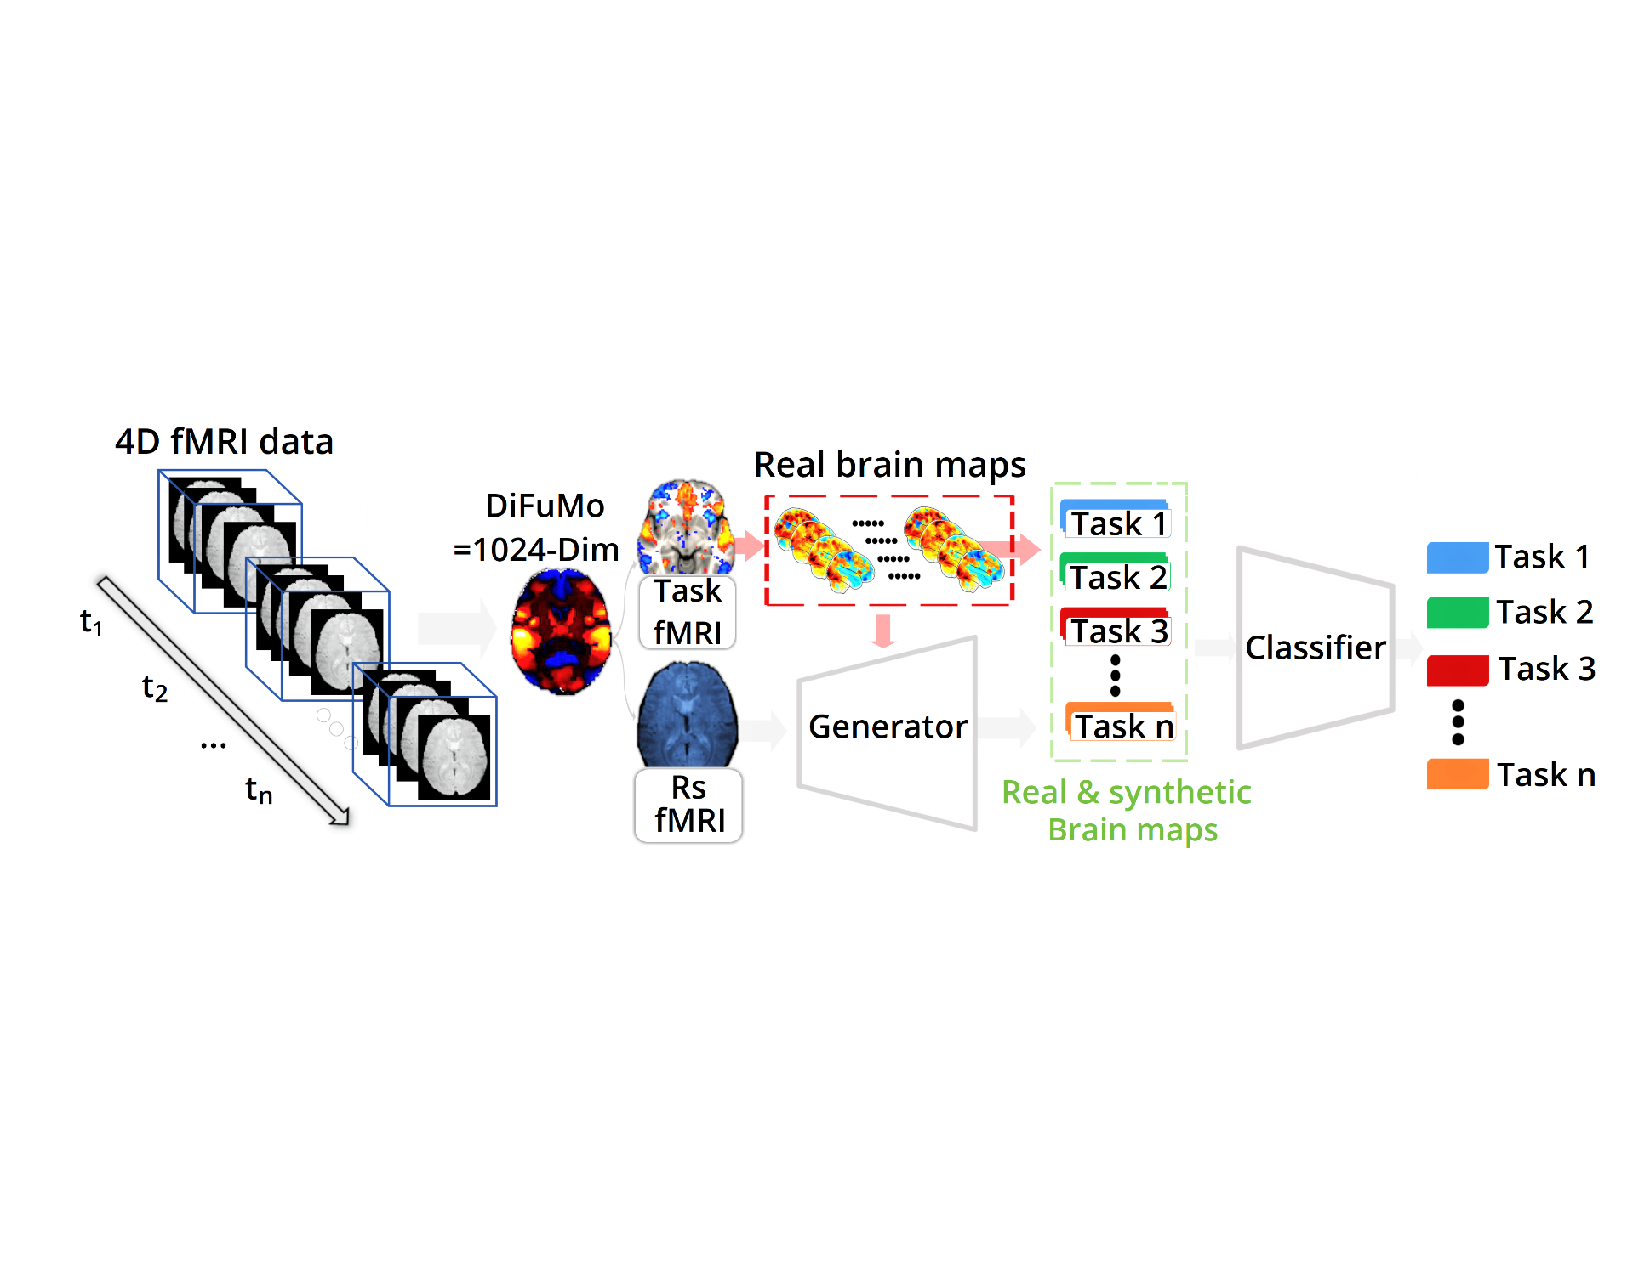
\includegraphics[width=1\textwidth]{condica/conceptual_figure_1_v6_redim.pdf}}
\caption{\textbf{Conditional ICA approach.} Our method aims to
  generate surrogate data from Task and Rest fMRI data by synthesizing
  statistical maps that qualitatively fit the distribution of the
  original maps. These can be used to improve the accuracy of
  machine learning models that identify contrasts from the
  corresponding brain activity patterns.}
\label{Fig0}
\end{figure}



\section{Methods}

\subsection{Spatial Dimension reduction.} 
The outline of the proposed approach is presented in Fig.\ref{Fig0}.
%
While brain maps are high-dimensional, they span a smaller space than that of
the voxel grid. 
%
For the sake of tractability, we reduce the dimension of the data by projecting the voxel values on the
high-resolution version of the Dictionaries of Functional Modes \emph{DiFuMo}
atlas \cite{dadi_fine-grain_2020}, i.e. with $p=1024$ components.
%
The choice of dimension reduction technique generally has an impact on the
results. However we consider this question to be out of the scope of the current study and leave this to future work.

\subsection{A generative model for task data}
Consider a task dataset $X^{task}$ in $\mathbb{R}^{p,n}$ where $n$ is the number of
data (samples) and $p=1024$ the number of components in the atlas. $X^{task}$ can be seen as $n$
observations of a random vector $\xb^{task} \in \RR^p$. Let us
consider how to learn the distribution of $\xb^{task}$. 
%
Assuming a Gaussian distribution is standard in this setting, yet, as
shown later, it misses key distributional features.
%
Moreover, we consider a model that subsumes the distribution of any type of
fMRI data (task or rest): a linear mixture of $k \leq p$ independent temporal signals.
%
We therefore use temporal ICA to learn a dimension reduction and unmixing matrix
$W^{task} \in \mathbb{R}^{k, p}$ such that the $k$ components i.e the $k$ components of
$W^{task} \xb^{task}$ are as
independent as possible.

A straightforward method to generate new task data would be to
independently sample them from the distribution of the components.
%
This is easy because such distribution has supposedly independent marginals.
We apply an invertible quantile transform $q^{task}$ to the components of $W^{task} \xb^{task}$ so that
the distribution of $q^{task}(W^{task} \xb^{task})$ has standardized Gaussian
marginals. Since it also has independent marginals it is given by $\mathcal{N}(\zero_k, I_k)$
from which we can easily sample.

However task datasets   have a small number of samples ($10 \sim 10^2$). As a
result, there are too few samples to learn high quality unmixing matrices. In
contrast, resting state datasets have a large number of samples ($10^4 \sim 10^5$).
Therefore we replace the unmixing matrix learned on task data $W^{task}$ by the
unmixing matrix learned on resting state data $W^{rest}$.
We therefore form $\zb^{task} = W^{rest} \xb^{task}$ and learn its quantile
transform $q$.

The encoding model is given by:
\begin{align}
  \zb^{task} = q(W^{rest} \xb^{task})
\end{align}

However, the independence assumption no longer holds and thus a latent structure among the marginals of
$\zb^{task}$ has to be taken into account. In addition the generative model needs
to be conditioned to each class. We therefore assume that the samples in class
$c$, $\xb_c^{task}$ are such that:
\begin{align}
q(W^{rest}\xb^{task}_c) \sim \Ncal( \mu_c, \Lambda)
\end{align}

In order to maximize the number of samples used to learn the parameters of the
model, we assume that the quantile transform $q$ and the latent covariance
$\Lambda$ do not depend on the class $c$. However, the mean $\mub_c$, that can be learned efficiently using just a few tens of samples, depends on class $c$.
$\Lambda$ is learned using all task samples from a standard shrunk covariance
estimator
$\Lambda = = \Sigma (1 - \alpha) + \frac{\alpha}{k} \tr(\Sigma) I_k$ where
$\alpha$ is given by the Ledoit-Wolf formula \cite{ledoit2004well} and
$\Sigma$ is the sample covariance of $\zb^{task}$.

The generative model of data for brain maps in a certain class $c$ is given by the pseudo inverse of the encoding model:
\begin{equation}
  \xb_c = (W^{rest})^{\dagger} q^{-1}(\epsilonb)
\end{equation}
with $\epsilonb \sim \mathcal{N}(\mub_c, \Lambda)$ and $(W^{rest})^{\dagger}$ is
the Moore Penrose inverse of $W^{rest}$

An overview of our generative method is shown in Fig.~\ref{Fig11}.
%
\begin{figure}
\centerline{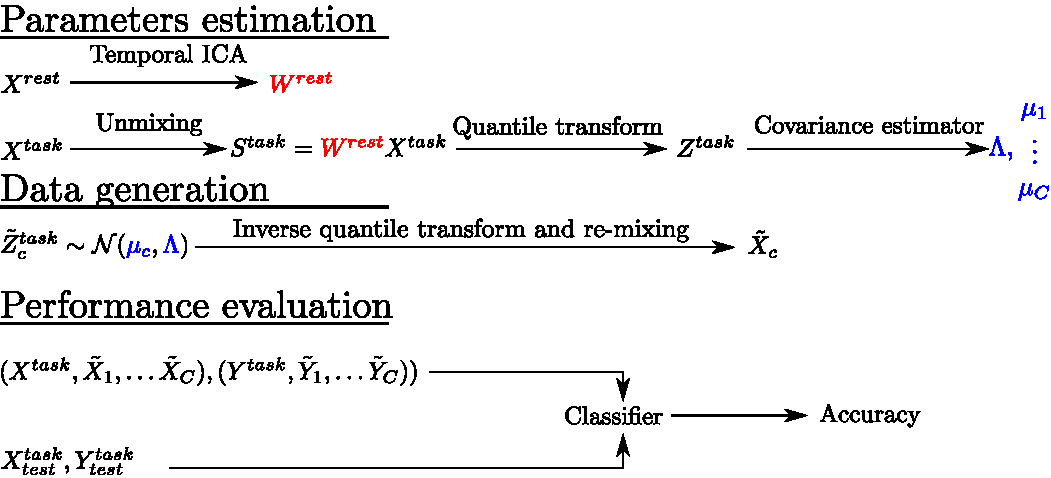
\includegraphics[width=1\textwidth]{figures/condica/method_figure}}
\caption{\textbf{Conditional ICA approach in depth.} 
The approach proceeds by learning a temporal ICA of rest data $X^{rest} \in
\mathbb{R}^{p, n}$ , resulting in
independent components and unmixing matrix $W^{rest} \in \mathbb{R}^{k, p}$.
%
Applying the unmixing matrix to the task data, we obtain samples in the component
space that we map to a normal distribution, yielding $Z^{task} \in
\mathbb{R}^{k, n}$. 
%
Then, we estimate the covariance $\Lambda \in \mathbb{R}^{k, k}$ (all classes are assumed to have the
same covariance) and the class-specific means $\boldsymbol{\mu}_1, \dots, \mub_C \in \mathbb{R}^{k}$ according to Ledoit-Wolf's method.
%
For each class $c$, we can draw random samples $\tilde{Z}^{task}_c \in
\mathbb{R}^{k, n_{\mathrm{fakes}}}$ from the
resulting multivariate Gaussian distribution $\mathcal{N}(\mub_c, \Lambda)$ and
obtain fake data $\tilde{X}_c  \in
\mathbb{R}^{p, n_{\mathrm{fakes}}}$
by applying the inverse quantile transform and re-mixing the data using the pseudo inverse of the unmixing matrix.
%
We append these synthetic data to the actual data to create our new augmented
dataset on which we train classifiers.}
\label{Fig11}
\end{figure}
%

\section{Related work}
In image processing, data augmentation is part of standard toolboxes and
typically includes operations like cropping, rotation, translation.
%
On fMRI data these methods do not make much sense as brain data are not invariant to such transformations.
%
More advanced techniques~\cite{zhuang2019fmri} %\cite{sandfort2019data}
are based on generative models such as GANs or variatonal
auto-encoders~\cite{kingma2013auto}. Although GAN-based method are powerful they are slow and difficult to train~\cite{arjovsky_wasserstein_2017}.

Our method is not an adversarial procedure, however it relates to other
powerful generative models such as variatonal
auto-encoders~\cite{kingma2013auto} with which it shares strong similarities.
Indeed the analog of the encoding function in the variational auto-encoder is
given by $e(\xb) = \Lambda^{-\frac12}q(W^{rest} \xb)$ in our model and the analog to the decoding
function in the variational auto-encoder is given by $d(\zb) =
(W^{rest})^{\dagger}q^{-1}(\Lambda^{\frac12}\zb)$ in our model. As in the variational auto-encoder, $e$ approximately maps the distribution of the data to a standardized Gaussian distribution,
while the reconstruction error defined by the difference in l2 norm
$\|d(e(\xb)) - \xb\|^2_2$ must remain small.
Lastly, another classical generative model related to ours is normalizing
flows.  We note that when $W^{rest}$ is square (no dimension reduction in ICA), the decoding operator $d$ is invertible (its inverse is $e$) making our
model an instance of normalizing flows~\cite{rezende2015variational}. 
%
A great property is thus the simplicity and reduced cost of data generation.

\section{Conclusion}
In this chapter, we introduced Conditional ICA, a fast generative model for task
data.
Conditional ICA is essentially a linear generative model with
pointwise non-linearity, which makes it cheap, easy to instantiate on new data,
and to introspect.
In the next chapter, we look at the performance of Conditional ICA on fMRI data.


\chapter{CondICA in practice}
\label{ch:condica2}
In the previous chapter, we have introduced Conditional ICA, a fast generative
model for task and rest fMRI data.
In this chapter, we first show that the generative model of resting state data shipped in Conditional ICA produces samples that neither linear nor non-linear classifiers are able to distinguish.
% 
Then we benchmark Conditional ICA as a generative model of task data against
various augmentation methods  on their
ability to improve classification accuracy on a large task fMRI dataset.
We find that Conditional ICA yields highest accuracy improvements.
In particular Conditional ICA outperforms GANs and conditional GANs~\cite{mirza2014conditional} while being much easier to optimize and interpret. 
Lastly, we show on 8 different datasets that the use of Conditional ICA results in systematic improvements in classification accuracy ranging from 1\% to 5\%.

\section{Dataset, data augmentation baselines and classifiers used}
\label{sec:condica:datasets}
The unmixing matrices are learned on the rest HCP
dataset~\cite{van2013wu} using 200 subjects.
These data were used after standard
preprocessing, including linear detrending, band-pass filtering
($[0.01, 0.1]Hz$) and standardization of the time courses.
The other 8 datasets~\cite{van2013wu, shafto2014cambridge,
  orfanos2017brainomics, pinel2019functional, pinel2007fast, pinel2013genetic,
  poldrack2016phenome, pinel2013genetic} are obtained from the Neurovault repository~\cite{gorgolewski2015neurovault}.
The classes used in each of these datasets correspond to the activation maps
related to contrasts (such as ``face vs tools'')
present in the set of tasks of each dataset. In table~\ref{fig:dataset:tab}, we
give references to the datasets used as well as the total number of samples
(subjects), the size of train and test sets in each of the cross validation
splits and the number of classes in each dataset. 

\begin{table}
\begin{center}
\begin{tabular}{c|c|c|c}
\hline
Dataset & Subjects, & Train/Test & Neurovault \\
 & classes  &  & collection 
\\ \hline
hcp~\cite{van2013wu}  & 787, 23 & 100/687  &  4337
\\
cam-can \cite{shafto2014cambridge}  & 605, 5 & 100/505  &  4342
\\
brainomics \cite{orfanos2017brainomics}  & 94, 19 & 50/44  &   4341
\\
archi \cite{pinel2019functional}  & 78, 30 & 40/38  &  4339
\\
la5c \cite{poldrack2016phenome}  & 191, 24 & 100/91  &  4343
\\
pinel2012archi \cite{pinel2019functional} & 76, 10 & 40/36  &  1952
\\
pinel2009twins \cite{pinel2013genetic}  & 65, 12 & 35/30  &  1952
\\
pinel2007fast \cite{pinel2007fast} & 133, 10 & 70/63  &  1952
\\\hline\hline
\end{tabular}
\end{center}
\caption{\textbf{Datasets used in the experiments.} The table provides
  references to the datasets that were used for our experiments, with
  the number of subjects, the number of classes, the number of subjects in train
  and test set in each cross validation split and the collection number in Neurovault}
  \label{fig:dataset:tab}
\end{table}


We consider 5 alternative
augmentation methods: \emph{ICA}, \emph{Covariance}, \emph{ICA + Covariance}, \emph{GANs} and \emph{CGANs}.
%
When no augmentation method is applied we use the label \emph{Original}.

The \emph{ICA} covariance method applies ICA to $X^{task}$ to generate unmixing matrices $W^{task}$ and
components $S^{task}=  W^{task} X^{task}$.
%
To generate a sample $\tilde{\xb}_c$ from class $c$, we sample
independently from each component restricted to the samples of class $c$ yielding $\tilde{\sbb}^{task}_c$ and mix the data: $\tilde{\xb}_c = (W^{task})^{\dagger}
\tilde{\sbb}^{task}_c$.
%

The \emph{Covariance} method generates a new sample of
synthetic data in class $c$ by sampling from a Multivariate Gaussian
with mean $\mub_c$ and covariance $\Sigma$, where $\mub_c$ is the
class mean and $\Sigma$ is the covariance of centered task data
estimated using Ledoit-Wolf method.
%
In brief, it assumes normality of the data per class.

The \emph{ICA + Covariance} method combines the augmentation
methods \emph{ICA} and \emph{Covariance}: samples are drawn following
the ICA approach, but with some additive non-isotropic Gaussian noise.
%
As in \emph{ICA} we estimate $W^{task}$ and $S^{task}$ from
$X^{task}$ via ICA.
%
Then we consider $R_{task} = X_{task} - W_{task} S_{task}$ and estimate the
covariance $\Sigma_R$ of $R_{task}$ via LedoitWolf's method.
%
We then generate a data sample $\tilde{\xb}_c$ from class $c$ as with ICA and add
Gaussian noise $\tilde{\nb} \sim \mathcal{N}(0,\Sigma_R)$.
%
Samples are thus generated as $\tilde{\xb}_c + \tilde{\nb}$.

The \emph{GANs} and \emph{CGANs}) methods rely on similar networks. The generator and discriminator have a mirrored architecture with 2 fully connected hidden layer of size (256 and 512).  The number of epochs, batch size, momentum and learning rate are set to 20k, 16, 0.9, 0.01 and we use the Leaky RELU activation function.

We evaluate the performance of augmentation methods through the use of classifiers: logistic regression (LogReg), linear
discriminant analysis with Ledoit-Wold estimate of covariance (LDA) perceptron
with two hidden layers (MLP) and random forrests (RF).
The hyper-parameters in each classifier are optimized through an internal 5-Fold
cross validation. We set the number of iterations in each classifier so that
convergence is reached. The exact specifications are given in table~\ref{fig:classifiers:tab}.

\begin{table}
  \begin{tabular}{ p{.11\textwidth} | p{.3\textwidth} |p{.5\textwidth}}
\hline
  Methods & Optimizer & Hyper-parameters \\
  \hline
LogReg & L-BFGS \newline ($20~000$ iterations) & inverse $L_2$ regularization
strength \newline in $\{0.0001, 0.001, 0.01, 0.1, 1 \}$ \\
  \hline
LDA  & Least-squares solver & Estimation of covariance \newline using Ledoit-Wolf's
                              method \\
  \hline
  RF &  - &  Default parameters in sklearn \\
  \hline
MLP  & Adam \newline ($20~000$ iterations, \newline momentum: $0.9$, \newline
batch size: $32$, \newline learning
       rate: $0.0001$) & $ReLU$ activation function, fully connected
                         architecture with two hidden layers both of size $1024$, L2
                         penalty coefficient: $10^{-5}$
\caption{\textbf{Optimizers and hyper-parameters of classifiers} For each classifier, we give the optimization method used as well as the value of hyper-parameters.}\label{fig:classifiers:tab} 
\end{tabular}
\end{table}


 
\section{Distinguish fake from real HCP resting state data}
This experiment is meant to assess the effectiveness of the data
augmentation scheme in producing good samples.
Data augmentation methods are trained on 200 subjects taken from HCP rest fMRI
dataset which amounts to $960k$ samples (4800
per individual). Then synthetic
data corresponding to $200$ synthetic subjects are produced, yielding
$960k$ fake samples and various classifiers are trained to distinguish fake from
real data using 5-Fold cross validation. The cross-validated accuracy is shown
in table~\ref{tab2}.
Interestingly, we observe a dissociation between linear models (LogReg
and LDA) that fail to discriminate between generated and actual data,
and non-linear models (MLP and RF) that can discriminate samples from
the alternative augmentation methods.
%
By contrast, all classifiers are at chance when Conditional ICA is used.

\begin{table}
\begin{center}
\begin{tabular}{c|cccc}
\hline
Models & LDA  & LogReg & Random Forest &  MLP 
\\ \hline
ICA   & 0.493 & 0.500 & 0.672 &  0.697
\\
Covariance   & 0.473 & 0.461 & 0.610 &  0.626
\\
ICA + Covariance   & 0.509 & 0.495 & 0.685 &  0.706
\\
GANs   & 0.501 & 0.498 & 0.592 &  0.607
\\
CGANs   & 0.498 &  0.493 & 0.579 & 0.604
\\\hline
\textbf{Conditional ICA}  & 0.503 & 0.489 & 0.512 &  0.523
\\\hline\hline
\end{tabular}
\end{center}
  \caption{\textbf{Distinguish fake from real HCP resting state data}
    We use HCP resting state data from $n=200$ subjects ($960k$ samples) and produce an equally
    large amount of fake data ($960k$ samples) using data augmentation methods.
    The table shows the 5-fold cross validated accuracy obtained with various
    classifiers. When Conditional ICA is used, all classifiers are at chance.
    %
    }\label{tab2}
\end{table}
%
\section{Comparing augmentation methods based on classification accuracy on task
  HCP dataset}
In order to compare the different augmentation methods, we measure their 
relative benefit in the context of multi-class classification.
We use 787 subjects from the HCP task dataset that contains 23 classes and
randomly split the dataset into a train set that contains 100 subjects and a test set
that contains 687 subjects. In each split we train augmentation methods on the
train set to generate fake samples corresponding to $200$ subjects.  
These samples are then appended to the train set, resulting in an
augmented train set on which the classifiers are trained. Results, displayed in
table~\ref{condica:tab3}, show that Conditional ICA always yields a higher accuracy
than when no augmentation method is applied. The gains are over 1\% on all
classifiers tested excepts with the random forest classifier which yields much
lower accuracy than other methods.
%
By contrast, ICA+Covariance and ICA lead to a decrease in accuracy
while the Covariance approach leads to non-significant
gains.
%

\begin{table}
  \setlength{\tabcolsep}{0.23em}
  % {\renewcommand{\arraystretch}{1}% for the vertical padding
  \begin{center}
    \begin{tabular}{c|c|c|c | c}
      \hline
      Models & LDA & LogReg & MLP& RF\\
      \hline
      Original           & 0.893 & 0.874 &  0.779 &0.782 \\
    ICA                & 0.814 & 0.840 &  0.803 &0.778\\
    Covariance         & 0.895 & 0.876 &  0.819 &0.780\\
    ICA + Covariance   & 0.816 & 0.840 &  0.815 &0.780\\
    GANs               & 0.877 & 0.863 &  0.771 &0.780\\
    CGANs              & 0.874 & 0.874 &   0.726&0.779 \\
    \hline                                      
      \textbf{Conditional ICA} &  \textbf{0.901} & \textbf{0.890} & \textbf{0.832} &  \textbf{0.783} \\
    \hline\hline
\end{tabular}
\end{center}
\caption{\textbf{Comparing augmentation methods based on classification accuracy on task
      HCP dataset} We compare augmentation methods based on the classification
    accuracy \textbf{(Acc)} obtained by 2 linear classifiers (LDA and LogReg) and two
    non-linear classifier (MLP and RF) trained on augmented datasets on HCP
    Task fMRI data. We report the mean accuracy across 5 splits.}
  \label{condica:tab3}
\end{table}

In table~\ref{app:runningtime:tab}, we give the running-time of GAN based
methods and Conditional ICA. This shows that in contrasts to deep learning based
methods, the computational over-head induced by CondICA is very low.
\begin{table}
  \begin{center}
    \begin{tabular}{|c|c|}
      \hline
      Methods & Running-time (secs)
      \\ \hline
      GANs  & 12948.2 ($\approx$ 3,60 hr)
      \\
      CGANs  & 11015.1 ($\approx$ 3,05 hr)
      \\
      \textbf{Conditional ICA}  & 62 s 
      \\
      \hline
    \end{tabular}
  \end{center}
  \caption{\textbf{Running time.} We display the running time of three methods used
    to generate synthetic data. Conditional ICA is several orders of magnitude faster than
    GANs or CGANs. In practice the computational over-head induced by Conditional ICA is negligible.}\label{app:runningtime:tab}
\end{table}

Lastly, we provide some visualization of fake examples produced by GANs, CGANs and Conditional ICA in figure~\ref{sec:visualization:fig}.
\begin{figure}
  \centerline{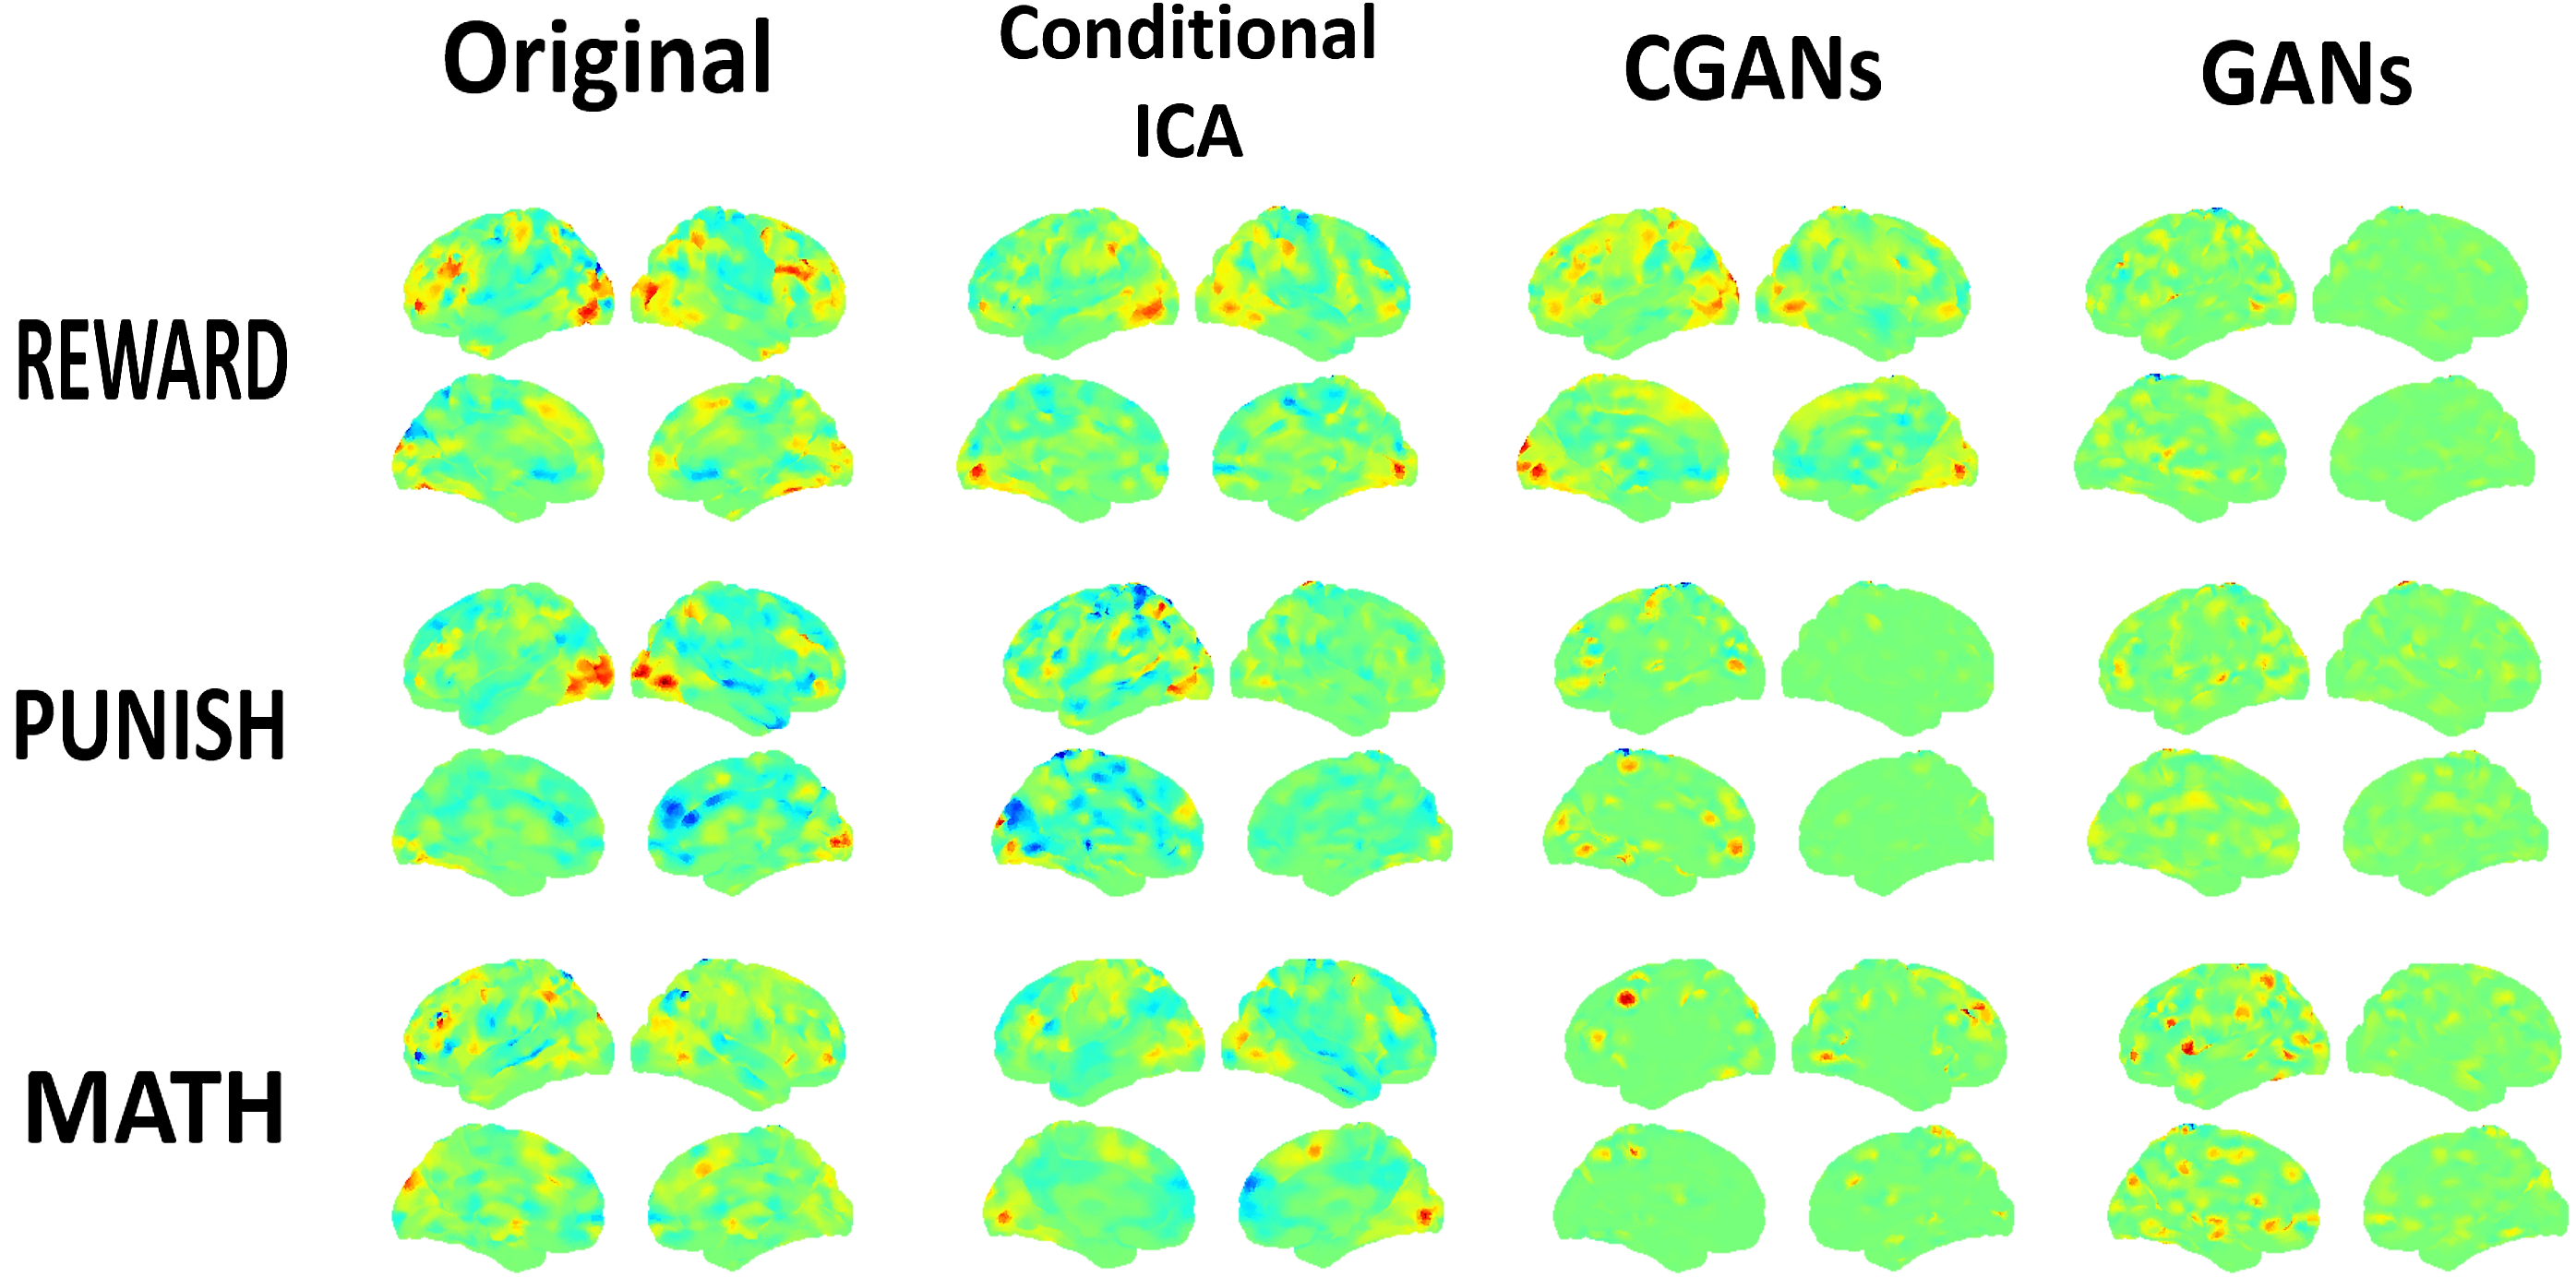
\includegraphics[width=0.8\linewidth]{figures/condica/fake_real_viz_v3_redim_improved.png}}
  \caption{\textbf{Data generation visualization.} Visualization of real
    (Original) and synthetic brain maps from three generation methods:
    Conditional ICA, CGANs and GANS. Three cognitive tasks are shown (reward, punish and math).
  }
  \label{sec:visualization:fig}
\end{figure}






\section{Gains in accuracy brought by conditional ICA on eight datasets.}
In this experiment we assess the gains brought by Conditional ICA data
augmentation on the eight different task fMRI datasets refered to in section~\ref{sec:condica:datasets}. The experimental pipeline is exactly the same as with the HCP task dataset.
We report in Fig.~\ref{Fig4} the cross-validated accuracy of
classifiers with and without augmentation.
We notice that the effect of data augmentation is
consistent across datasets, classifiers and splits, with 1\% to 5\% net gains.
%
\begin{figure}
  \centering
  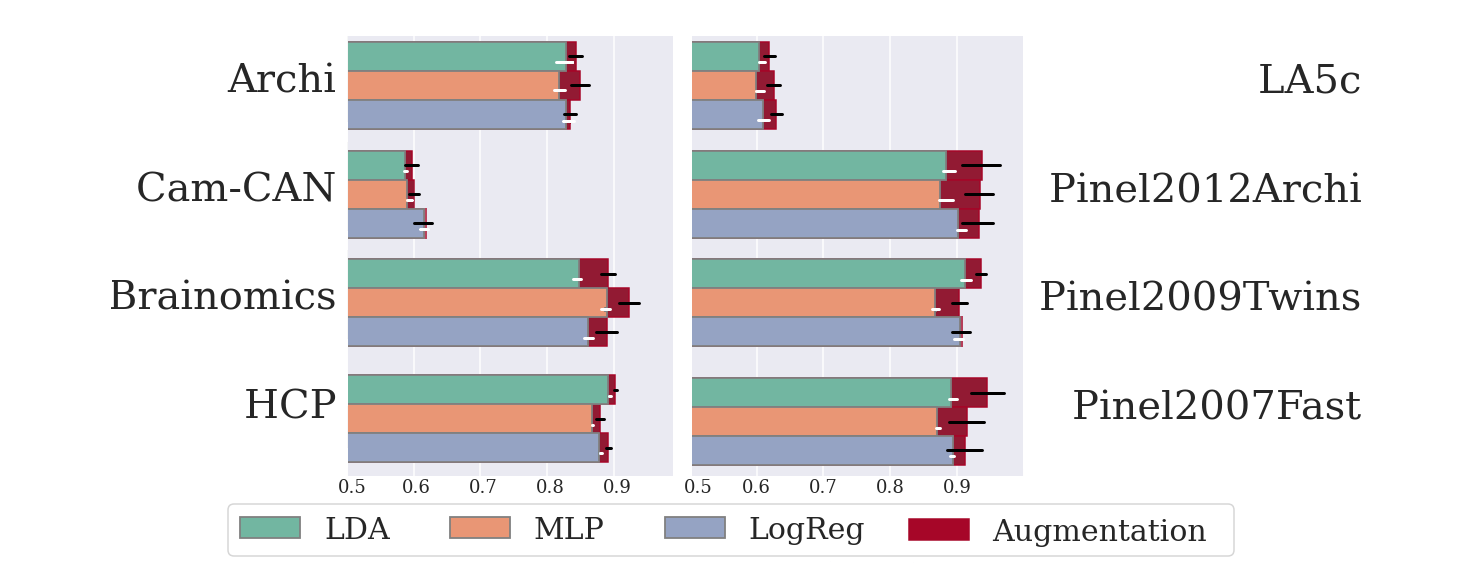
\includegraphics[width=\textwidth]{figures/condica/accuracy_all_datasets_v5.png}
\caption{\textbf{Accuracy of models for eight multi-contrast datasets.} Cross
  validated accuracy of two linear (LDA and LogReg) and one non-linear
  classifier (MLP) with or without using data augmentation.
  %
  The improvement yielded by data augmentation is displayed in red.
  %
  Black error bars indicate standard deviation across splits while white error bars indicate standard deviation across splits with no augmentation.}
\label{Fig4}
\end{figure}
%

Lastly, we provide a sensitivity analysis on the number of components used in
CondICA in figure~\ref{condica:sensitivity:fig}.
CondICA gives good performance for numbers of components between 800 and 1000
components. In all experiments we used $k=900$ components.

\begin{figure}
  \centerline{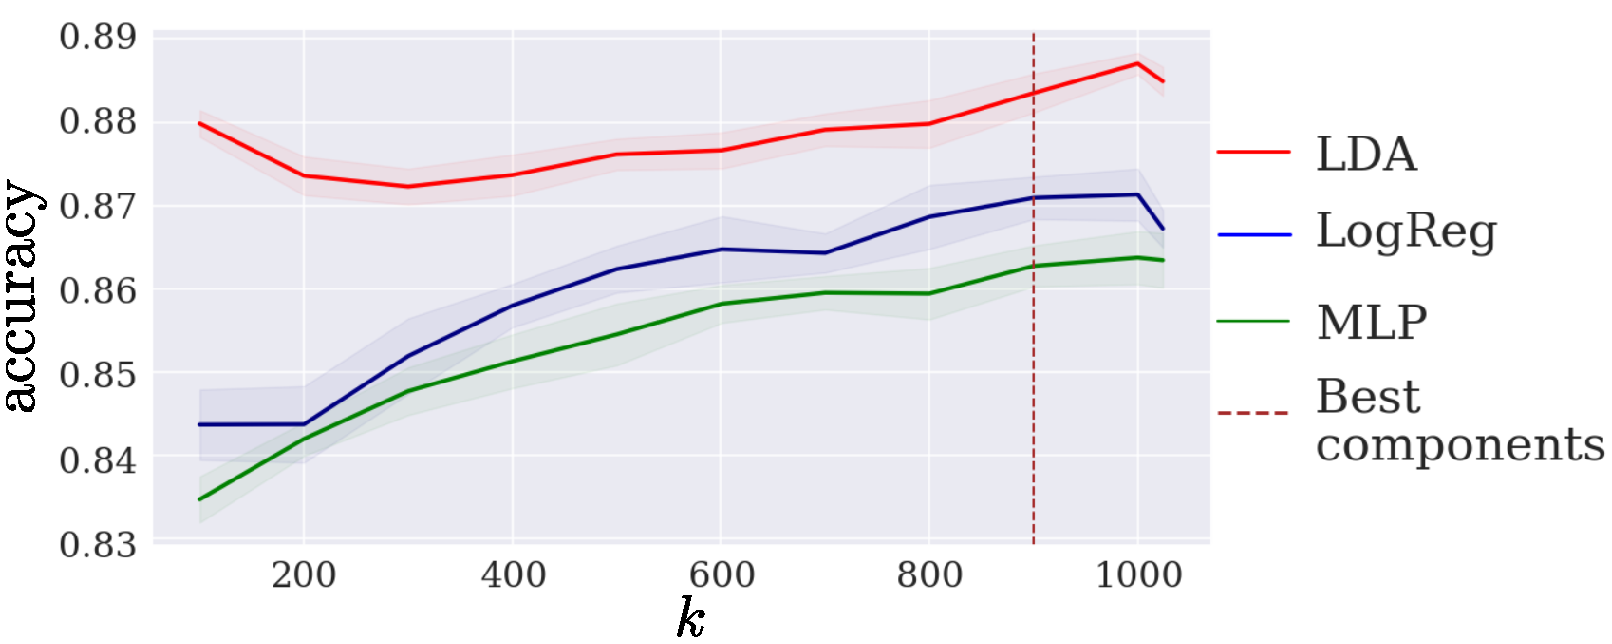
\includegraphics[width=0.8\textwidth]{figures/condica/sensitivity.pdf}}
  \caption{\textbf{Accuracy of augmented discriminative models when
      varying $k$.} We use 100 train subjects from the HCP task dataset to train Conditional ICA with $k$ components and generate $200$ fake subjects.
    Classifiers are trained on the train and fake subjects and tested on the
    left-out 687 subjects. We repeat the procedure
    for various values of $k$ using 5 random splits per value and
    report the mean accuracy across splits as a function of $k$.
    The dotted line represents the number of components that has been
    used in our experiments ($k=900$).
  }
  \label{condica:sensitivity:fig}
\end{figure}






\section{Conclusion}
Conditional ICA produces samples that cannot be distinguished from true actual rest by linear as well as non-linear classifiers, showing that it captures higher-order statistics than naive ICA-based generators.
%
When Conditional ICA is used as a data augmentation method, it yields consistent
improvement in classification accuracy: on 8 tasks fMRI datasets, we observe
increase in accuracy between 1\% and 5\% depending on the dataset and the
classifier used.
Importantly, this performance was obtained without any fine-tuning of
the method, showing its reliability. One can also notice that our experiments cover datasets with different cardinalities, from tens to thousand, and different baseline prediction accuracy.

The systematic performance improvement CanICA yields
makes it a promising candidate for data augmentation in a wide range of
contexts. Future work may focus on its applicability to other decoding tasks
such as the diagnosis of Autism Spectrum Disorder
(ASD)~\cite{eslami2019asd,eslami2019auto,dvornek2017identifying} or
Attention-Deficit/Hyperactivity Disorder detection (ADHD)~\cite{mao2019spatio}. Other extensions of the present work concern the adaptation to
individual feature (e.g. age) prediction where
fMRI has shown some potential.
%

\part{Conclusion}

\section{A note about resources used}
All the code is written in Python.
We use Matplotlib for plotting~\cite{hunter2007matplotlib} , scikit-learn for
machine-learning pipelines~\cite{pedregosa2011scikit}, MNE for MEG
processing~\cite{gramfort2013meg}, Nilearn for fMRI processing and for its CanICA implementation~\cite{abraham2014machine}, Brainiak~\cite{kumar2020brainiak} for its SRM implementation. 


\section{Contributions outside of the scope of the thesis}
Some of the contributions we have made during the thesis were outside of its
scope. We now present these contributions succinctly.

\subsection{A deep approach to model complex stimuli}
In this work, we learn a model to predict fMRI data of subjects watching a movie
from the activities of a deep neural network exposed to the same movie. The neural network is previously trained to perform action recognition on a large corpus of movies.
The association of activity in visual areas with the different layers of the
deep architecture displays complexity-related contrasts across visual areas and
reveals a striking foveal/peripheral dichotomy.

\paragraph{Published work}
\fullcite{richard2018optimizing}

\subsection{Predicting resting state from fMRI}
In this work, we predict task contrasts from rest fMRI data using a piecewise
  linear model. This model is shown to outperform linear models and a fully
  connected neural network.

  
\paragraph{Published work}
\fullcite{dohmatob2021brain}

\subsection{An optimal transport approach to hyperalignment}
In this work, we benchmark optimal transport, ridge regression and scaled
Procrustes to align the data of two
subjects. Optimal Transport Ridge regression seems to be the best method.

\paragraph{Published work}
\fullcite{bazeille2019local}


\chapter{Conclusion}
In this thesis, we have presented three contributions that allow to tackle
inter-subject variability in neuroimaging, and a data augmentation method for fMRI data.

First, in chapter~\ref{ch:fastsrm1} and chapter~\ref{ch:fastsrm2}, we develop an
atlas based procedure that is shown to accelerate significantly the existing
procedure for performing dimension reduction of fMRI data in a multi-subject
context with provably no loss of performance. It is now possible to apply these
algorithms in big datasets where the number of subjects is of the order of
several hundreds, with several thousand samples and several hundred thousand features.

Then, we propose in chapter~\ref{ch:mvica1} and chapter~\ref{ch:mvica2}
a novel unsupervised algorithm, MultiViewICA, that reveals latent sources observed through different views. Using an independence assumption, we have demonstrated that the model is identifiable, provided that the latent
sources are not Gaussian. In contrast to previous approaches, the proposed model leads to a closed-form likelihood, which we then optimize efficiently using a dedicated alternate quasi-Newton approach.
Therefore, our approach enjoys the statistical guarantees of maximum-likelihood
theory, while still being tractable. MultiViewICA outperforms other unsupervised
methods used in fMRI and MEG in the context of shared response modeling. However,
it assumes the same level of noise for all
subjects, which does not model properly between-subjects variability.

In chapter~\ref{ch:shica1} and chapter~\ref{ch:shica2}, we extend MultiViewICA so
[Omitted long matching line]
In practice ShICA outperforms MVICA and other unsupervised methods used in the
context of shared response modeling.

Lastly, we introduce in chapter~\ref{ch:condica1} and chapter~\ref{ch:condica2} a data
augmentation method based on ICA that outperforms deep learning algorithms in
terms of decoding accuracy while being much faster.

Combined with the FastSRM algorithm, MultiViewICA and ShICA yield a novel way to
make use of multi-view data. They yield a set of operators per view that map
the data of each view to a shared response reducing the variability between views.
In principle, reducing the variability between views should facilitate the
understanding of the data. In particular, it should be easier to perform
decoding from multiple subjects when the inter-subject variability is lower.
This direction could be explored in future work.

More generally, applications in this thesis were geared towards naturalistic imaging where the temporal response is assumed to be shared
across subjects. This is not a requirement of our methods and we see at least two other
settings in which our methods would be useful. The first
one is the analysis of resting state data assuming that spatial topographies are
shared across subjects. In this setting, the spatial topographies become the
common components while the mixing operators denote a set of time-courses. In
practice, the experimenter can perform such task by applying our method on
transposed data.
The second setting in which our methods could be useful is the analysis of MEG / EEG data assuming both a spatial and
temporal mixing. This can be done in practice by stacking the features of
consecutive samples.

In terms of methods, we have treated separately dimension reduction
(chapter~\ref{ch:fastsrm1}) and source identification (chapter~\ref{ch:mvica1}
and chapter~\ref{ch:shica1}). Future work might focus on understanding how these
two steps can be performed jointly. Lastly, in the case of naturalistic stimuli,
the mixing matrices represent spatial topographies and therefore they can be
assumed to be close to each other. This aspect is not addressed in our work
where no link is assumed between mixing matrices and could be the topic of
future research.




% 

\cleardoublepage%********************************************************************
% Bibliography
%*******************************************************
% work-around to have small caps also here in the headline
% https://tex.stackexchange.com/questions/188126/wrong-header-in-bibliography-classicthesis
% Thanks to Enrico Gregorio
\defbibheading{bibintoc}[\bibname]{%
  \phantomsection
  \manualmark
  \markboth{\spacedlowsmallcaps{#1}}{\spacedlowsmallcaps{#1}}%
  \addtocontents{toc}{\protect\vspace{\beforebibskip}}%
  \addcontentsline{toc}{chapter}{\tocEntry{#1}}%
  \chapter*{#1}%
}
\printbibliography[heading=bibintoc]

% Old version, will be removed later
% work-around to have small caps also here in the headline
%\manualmark
%\markboth{\spacedlowsmallcaps{\bibname}}{\spacedlowsmallcaps{\bibname}} % work-around to have small caps also
%\phantomsection
%\refstepcounter{dummy}
%\addtocontents{toc}{\protect\vspace{\beforebibskip}} % to have the bib a bit from the rest in the toc
%\addcontentsline{toc}{chapter}{\tocEntry{\bibname}}
%\label{app:bibliography}
%\printbibliography


\appendix
\part{Appendices}
\chapter{MultiViewICA}
\section{Proofs of Section~\ref{sec:mvica}}
\label{sec:app_proofs}
\subsection{Proof of Prop.~\ref{prop:identifiability}}
\label{app:proof:mvica:identifiability}
We fix a subject $i$. Since $\sbb$ has independent components, so does $\sbb + \nb_i$. Following~\cite{comon1994independent},
Theorem 11, there exists a scale-permutation matrix $P^i$ such that $A'_i =
A_iP^i$. As a consequence, we have $\sbb  + \nb_i = P^i(\sbb' + \nb'^i)$ for all
$i$.

Then, we focus on subject 1 and subject $i \neq 1$:
\begin{align}
  &\sbb + \nb^1 - (\sbb + \nb_i) = P^1(\sbb' + \nb'^1) - P^i(\sbb' + \nb'^i)\\
  &\nb^1 - \nb_i = P^1(\sbb' + \nb'^1) - P^i(\sbb' + \nb'^i)\\
  &\iff P^1\sbb' - P^i\sbb' = P^i \nb'^i - \nb_i + \nb^1 - P^1 \nb'^1 \label{eq:condition_Gaussian}
\end{align}
% This shows that $P^1\sbb' - P^i\sbb'$ is Gaussian which can only happen if $P^1= P^i$. 
Since the right hand side of equation (\ref{eq:condition_Gaussian}) is a linear combination of Gaussian random variables, this would imply that $P^1\sbb' - P^i\sbb'$ is also Gaussian. However, given that $\sbb'$ is assumed to be non-Gaussian, the equality can only hold if $P^1
= P^i$ and both the right and the left hand side vanish.
Therefore, the matrices $P^i$ are all equal, and there exists a scale and permutation matrix $P$ such that $A'_i = A_iP$.

\subsection{Proof of Prop.~\ref{prop:robust}}
\label{ref:robust}
We consider $W_i = \Lambda (A_i)^{-1}$, where $\Lambda$ is a diagonal matrix.
%
We recall $\xb_i= A_i (\sbb + \nb_i),$ so that $\yb_i = W_i\xb_i= \Lambda(\sbb + \nb_i)$.
%
The gradient of $\loss$ is given by equation~\eqref{eq:gradient}:
\begin{align*}
  \mathcal{G}^i &= \frac{1}{m}\EE[f'(\tilde{\sbb})(\sbb + \nb_i)^{\top}]\Lambda \\ & \enspace \enspace+ \frac{1 - 1/m}{\sigma^2} \Lambda\EE[\left(\nb_i - \frac{1}{m-1}\sum_{j\neq i} \nb^j\right)(\sbb + \nb_i)^{\top}]\Lambda - I_p \\
  & = \frac{1}{m}\EE[f'(\Lambda(\sbb + \frac1m\sum_j\nb^j))(\sbb+\nb_i)^{\top}] \Lambda + \frac{\sigma'^2(1 - 1/m)}{\sigma^2} \Lambda^2 - I_p
    \numberthis
\end{align*}
where we write $f'(\sbb) = \begin{bmatrix}f'(s_1) \\ \vdots \\ f'(s_p) \end{bmatrix}$.
Therefore, $\mathcal{G}^i$ is diagonal and constant across subjects (because $\EE[f'(\Lambda(\sbb + \frac1m\sum_j\nb^j))(\nb_i)^{\top}] = \EE[f'(\Lambda(\sbb + \frac1m\sum_j\nb^j))(\nb^{i'})^{\top}]$).
Let us therefore consider only its coefficient $(a, a)$, and let $\lambda = \Lambda_{aa}$:
$$
\mathcal{G}^i_{aa} =G(\lambda) = \phi(\lambda)\lambda + \frac{\sigma'^2(1 - 1/m)}{\sigma^2}\lambda^2 - 1,
$$
where $\phi(\lambda) = \frac{1}{m}\EE[f'(\lambda(s_a + \frac1m\sum_j n^j_a))(s_a+n_a^i)]$. One the one hand, we have $G(0) = -1$. On the other hand, if we assume for instance that $f'$ has sub linear growth (i.e. $|f'(x)| \leq c|x|^{\alpha} +d$ for some $\alpha < 1$) or that $\phi$ is positive, we find that $G(+\infty) = +\infty$.
Therefore, $G$ cancels, which concludes the proof.

\subsection{Stability conditions}
\label{sec:stability}
We consider $W_i = \Lambda (A_i)^{-1}$ where $\Lambda$ is such that the gradients $\mathcal{G}^i$ all cancel. We consider a small relative perturbation of $W_i $ of the form $W_i \leftarrow (I_p + E^i)W_i$, and consider the effect on the gradient.
We define $\Delta^i=\mathcal{G}^i\left((I_p + E^1)W_1, \dots, (I_p + E^m)W_m\right)$.
Denoting $C = \frac{1 - 1/ m}{\sigma^2}$ and $\tilde{\nb} = \frac1m\sum_{i=1}^m \nb_i$, we find:
\begin{align*}
  \Delta^i = \Delta^i_1 + C\Delta^i_2 - I_p
\end{align*}

where
\begin{align*}
     &\Delta^i_1= \\&\EE[\frac1m f'\left(\Lambda(\sbb + \tilde{\nb}) + \frac1m \sum_{j=1}^m E^j\Lambda(\sbb +\nb^j)\right)(\sbb +\nb_i)^{\top}\Lambda(I_p + E^i)^{\top}] \numberthis
 \end{align*}
 and
 \begin{align*}
   &\Delta^i_2= \EE[\left(\Lambda\nb_i - \frac{1}{m-1}\sum_{j\neq i} \Lambda\nbb^j + E^i\Lambda(\sbb + \nb_i) \right. \\& \left. - \frac{1}{m-1}\sum_{j\neq i} E^j \Lambda(\sbb + \nb^j)\right)(\sbb + \nb_i)^{\top}\Lambda(I_p + E^i)^{\top}]
   \numberthis
\end{align*}

The first term is expanded at the first order, denoting $S = \sum_{j=1}^m E^j$:

\begin{align*}
  \Delta_1^i &= \EE[\frac1m \Bigg( f''(\Lambda(\sbb + \tilde{\nb}))\odot \big(\frac1m \sum_{j=1}^m E^j\Lambda(\sbb +\nb^j)\big) \\& + f'(\Lambda(\sbb + \tilde{\nb})) \Bigg) (\sbb +\nb_i)^{\top}\Lambda(I_p + E^i)^{\top}]\\
    &=\EE[\frac1m f'(\Lambda(\sbb + \tilde{\nb}))(\sbb + \nb_i)^{\top}\Lambda(I_p + E^i)^{\top} \\&+ \frac1{m^2}S\odot  \left(f''(\Lambda(\sbb + \tilde{\nb}))(\sbb^2)^{\top}\Lambda^2 \right)\\
    &+\frac{1}{m^2}E^i\odot\left(f''(\Lambda(\sbb + \tilde{\nb}))((\nb_i)^2)^{\top}\Lambda^2 \right)]
      \numberthis
\end{align*}
The symbol $\odot$ denotes the element-wise multiplication, $f'(\sbb) = \begin{bmatrix}f'(s_1) \\ \vdots \\ f'(s_p) \end{bmatrix}$ and $f''(\sbb) = \begin{bmatrix}f''(s_1) \\ \vdots \\ f''(s_p) \end{bmatrix}$.
Similarly, the second term gives at the first order: 
\begin{align}
    \Delta_2^i &= \EE[\sigma'^2\Lambda^2(I_p + E^i)^{\top} + (1 + \sigma'^2)E^i\Lambda^2 - \frac{1}{m-1} (S - E^i) \Lambda^2]
\end{align}

Combining this, we find:

\begin{align}
 \Delta^i = (E^i)^{\top} + E^i \odot\Gamma^E
 +S\odot \Gamma^S
\end{align}
where 
$$
\Gamma^E= \left(\frac1{m^2}\EE[f''(\Lambda(\sbb + \tilde{\nb}))((\nb_i)^2)^{\top}] + (1-\frac1m)\frac{\sigma'^2}{\sigma^2} + \frac{1}{\sigma^2} \right)\Lambda^2
$$
$$
\Gamma^S =\left(\frac1{m^2}\EE[f''(\Lambda(\sbb + \tilde{\nb}))(\sbb^2)^{\top}] -\frac{1}{m\sigma^2}  \right)\Lambda^2
$$

are $p\times p$ matrices, independent of the subject.
This linear operator is the Hessian block corresponding to the $i$-th subject:
Denoting $\mathcal{H}$ the Hessian, it is the mapping $\mathcal{H}(E^1, \dots, E^m) = (\Delta^1, \dots, \Delta^m)$.

The coefficient $\Delta^i_{ab}$ only depends on $(E^i_{ab}, E^i_{ba}, E^1_{ab},\dots, E^m_{ab})$. Therefore, the Hessian is block diagonal with respect to the blocks of coordinates $(E^1_{ab}, E^1_{ba}, \dots, E^m_{ab}, E^m_{ba})$. Denote $\varepsilon = \Gamma^E_{ab}$, $\varepsilon' = \Gamma^E_{ba}$, $\beta = \Gamma^S_{ab}$ and $\beta'= \Gamma^S_{ba}$. The linear operator for the block is:

\begin{align*}
&K(\varepsilon, \varepsilon', \beta, \beta')= \\
&\left(
    \begin{array}{ll|ll|l|ll}
\varepsilon + \beta & 1       & \beta & 0       & \dots  & \beta & 0       \\
1      & \varepsilon' + \beta' & 0      & \beta' & \dots  & 0      & \beta' \\
\hline
\beta & 0       & \varepsilon + \beta & 1       &        & \beta & 0       \\
0      & \beta' & 1      & \varepsilon' + \beta' & \ddots & 0      & \beta' \\
\hline
\vdots & \vdots  &        & \ddots  & \ddots & \vdots & \vdots  \\
\hline
\beta & 0       & \beta & 0       & \dots  & \varepsilon + \beta & 1       \\
0      & \beta' & 0      & \beta' & \dots  & 1      & \varepsilon' + \beta'
    \end{array}
\right)
\end{align*}
The positivity of $\mathcal{H}$ is equivalent to the positivity of this operator for all pairs $a, b$.
We now assume $\beta \beta' > 0$.

First, we should note that $K(\varepsilon, \varepsilon', \beta, \beta') $ is
congruent to $K(\varepsilon \sqrt{\frac{\beta'}{\beta}}, \varepsilon'
\sqrt{\frac{\beta}{\beta'}}, \sqrt{\beta\beta'}, \sqrt{\beta\beta'})$ via the
basis \\ $\text{diag}((\frac{\beta'}{\beta})^{1/4}, (\frac{\beta}{\beta'})^{1/4}, \cdots,(\frac{\beta'}{\beta})^{1/4}, (\frac{\beta}{\beta'})^{1/4})$.
%
We denote to simplify notation $\alpha = \varepsilon \sqrt{\frac{\beta'}{\beta}}$, $\alpha' = \varepsilon' \sqrt{\frac{\beta}{\beta'}}$ and $\gamma = \sqrt{\beta\beta'}$. We only have to study the positivity of $K(\alpha, \alpha', \gamma, \gamma)$.
We have:
$$
K(\alpha, \alpha', \gamma, \gamma) =  I_m  \otimes M_\alpha+ \gamma  \mathbb{1}\otimes I_2, \enspace M_\alpha = 
\begin{pmatrix}
\alpha & 1 \\
1 & \alpha'
\end{pmatrix}
$$
Since $I_m\otimes M_\alpha$ and $\gamma \mathbb{1}\otimes I_2$ commute, the minimum value of $\text{Sp}(K)$ is $\text{min}(I_m\otimes M_\alpha) + \text{min}(\gamma\text{Sp}(\mathbb{1}))=\frac12(\alpha + \alpha' - \sqrt{(\alpha - \alpha')^2 + 4}) + m\min(0, \gamma)$.
Since we assumed $\beta \beta' > 0$ we have $\gamma > 0$. This is similar to the usual ICA case, we find that the condition is $\alpha\alpha' > 1$.

If the following conditions hold for all pair of components $a, b$, the components are a local minimum of the cost function:
\begin{itemize}
    \item $\Gamma^S_{ab}\Gamma^S_{ba}\geq 0$
    \item $\Gamma^E_{ab}\Gamma^E_{ba} > 1$
\end{itemize}
% \section{Identifiability for Shared Response Model}
% \label{sec:app_identifiability}
% The shared response model~\cite{chen2015reduced} (SRM) models the data $\xb_i \in \bbR^v$ of subject $i$ for $i = 1,\dots, m$ as
% \begin{align*}
%     \xb_i = A_i \sbb + \nb_i \enspace \text{with} \enspace \sbb \sim \Ncal(0, \Sigma), \enspace\nb_i \sim \Ncal(0, \rho_i^2 I_v), \enspace {A_i}^{\top}A_i = I_p
% \end{align*}
% where $A_i \in \bbR^{v, k}$, $\sbb \in \bbR^p$ and  $\Sigma \in \mathbb{R}^{k, k}$ is a symmetric positive definite matrix.

% \begin{proposition}
% SRM is not identifiable
% \end{proposition}
% \begin{proof}
% Let us assume the data $\xb_i \enspace i=1, \dots, m$ follow the SRM model with parameters $\Sigma, A_i, \rho_i^2 \enspace i=1, \dots, m$. 

% Let us consider an orthogonal matrix $O \in \Ocal_k$.
% We call $A'_i = A_i O$ and $\Sigma' = O^{\top} \Sigma O$. 
% $\Sigma'$ is trivially symmetric positive definite.

% Then the data also follows the SRM model with different parameters $\Sigma', A'_i, \rho_i^2 \enspace i=1, \dots, m$.
% \end{proof}

% \begin{proposition}
% We consider the decorrelated SRM model with an additional decorrelation assumption on the shared responses.
% \begin{align*}
% \xb_i = A_i \sbb + \nb_i \enspace \text{with} \enspace \sbb \sim \Ncal(0, \Sigma), \enspace\nb_i \sim \Ncal(0, \rho_i^2 I_v), \enspace {A_i}^{\top}A_i = I_p
% \end{align*}
% where $\Sigma$ is a positive \emph{diagonal} matrix. We further assume that the values in $\Sigma$ are all distinct and ranked in ascending order.
% The decorrelated SRM is identifiable up to sign indeterminacies on the columns of 
% $\begin{bmatrix}
% A_1 \\
% \vdots \\
% A_m
% \end{bmatrix}
% $.
% \end{proposition}
% \begin{proof}
% The decorrelated SRM model can be written
% \begin{align*}
%     &\xb_i \sim \Ncal(0, A_i \Sigma {A_i}^{\top} + \rho_i^2 I_v) \enspace \text{with}\enspace  {A_i}^{\top}A_i = I_p
% \end{align*}
% where $\Sigma$ is a positive diagonal matrix with distincts values ranked in ascending order.

% Let us assume the data $\xb_i \enspace i=1, \dots, m$ follow the decorrelated SRM model with parameters $\Sigma, A_i, {\rho_i}^2 \enspace i=1, \dots, m$. Let us further assume that the data $\xb_i \enspace i=1, \dots, m$ follow the decorrelated SRM model with an other set of parameters $\Sigma', A'_i, {\rho'_i}^2 \enspace i=1, \dots, m$.

% Since the model is Gaussian, we look at the covariances.
% We have for $i \neq j$
% \begin{align*}
%     \bbE[\xb_i\left(\xb_j\right)^{\top}] = A_i\Sigma {A_j}^{\top} = A'_i \Sigma'{A'_j}^{\top} \enspace, 
% \end{align*}
% The singular value decomposition is unique up to sign flips and permutation. Since eigenvalues are positive and ranked the only indeterminacies left are on the eigenvectors. For each eigenvalue a sign flip can occur simultaneously on the corresponding left and right eigenvector.

% Therefore we have $\Sigma' = \Sigma$, $A_i = A'_i D_{ij}$ and $A_j = A'_j D_{ij}$ where $D_{ij} \in \bbR^{k, k}$ is a diagonal matrix with values in $\{-1, 1\}$. This analysis holds for every $j \neq i$ and therefore $D_{ij} = D$ is the same for all subjects.

% We also have for all $i$
% \begin{align*}
%     \bbE[\xb_i \left(\xb_i\right)^{\top}] = A_i \Sigma {A_i}^{\top} + \rho_i^2 I_v =  A'_i \Sigma' {A'_i}^{\top}  + {\rho'}_i^2 I_v\\
% \end{align*}
% We therefore conclude ${\rho'}_i^2 = \rho_i^2, i=1 \dots m$.

% Note that if the diagonal subject specific noise covariance $\rho_i^2 I_v$ is replaced by any positive definite matrix, the model still enjoys identifiability.
% \end{proof}

\subsection{Reproducing time-segment matching experiment}
\label{appendix_reproduce}
We reproduce the time-segment matching experiments described in \cite{chen2016convolutional} and \cite{zhang2016searchlight} and use two fold classification over runs instead of 5-fold as we have done in chapter~\ref{ch:mvica2}. We used the sherlock data available at \url{http://arks.princeton.edu/ark:/88435/dsp01nz8062179} and the full brain mask provided in the Python package associated with the paper. We applied high-pass filtering (140 s cutoff) and the time series of each voxel were normalized to zero mean and unit variance.

The results are available in Figure~\ref{fig:supp_timesegment}.

\begin{figure}
  \centering
  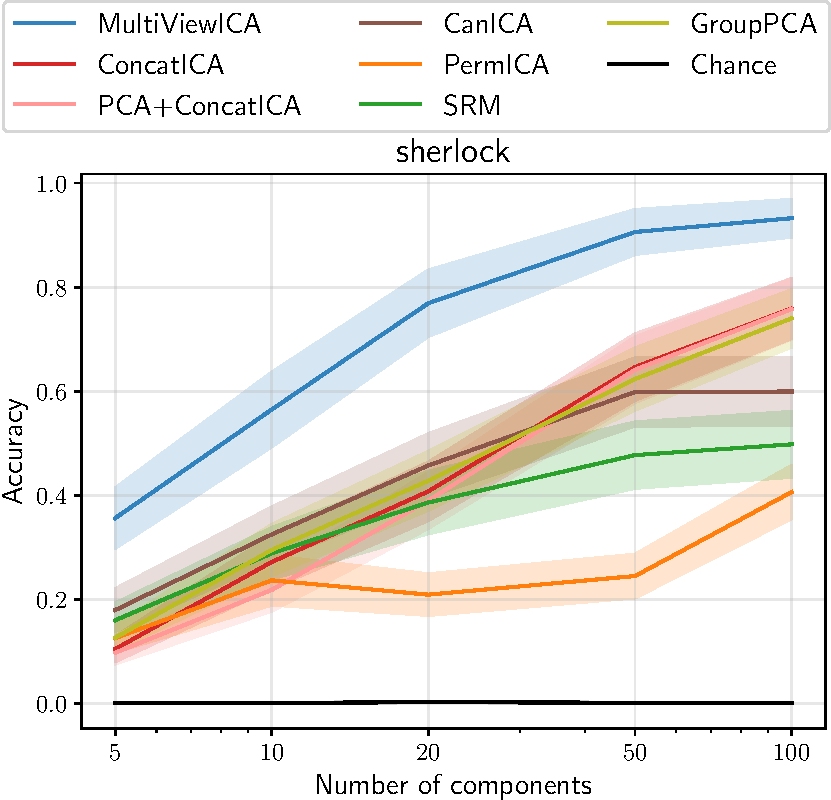
\includegraphics[width=0.6\textwidth]{figures/mvica/timesegment_matching_cae.pdf}
  \caption{\textbf{Reproducing the time-segment matching experiment of \cite{chen2016convolutional}~\cite{zhang2016searchlight}} Mean classification accuracy - error bars represent 95\% confidence interval}
  \label{fig:supp_timesegment}
\end{figure}

\section{Related Work}
\label{sec:app_rel_work}
The following table describes some usual method for extracting shared components from multiple subjects datasets.
The column "Modality/Components" describes the type of data for which each algorithm was \emph{initially} proposed, even though each algorithm could be applied on any type of data. 
%
The components type can be either temporal if extracted components are time courses or spatial if they are spatial patterns. 
%
\begin{center}
\begin{longtable}{ |p{.25\textwidth} | p{.17\textwidth} |p{.2\textwidth}| p{.24\textwidth}|}
\hline
\textbf{Method} & \textbf{Modality / Components} &\textbf{Dimension reduction} & \textbf{Description}  \\
\hline
SRM \cite{chen2015reduced} & 
fMRI / Temporal
&
SRM
&
The model is $\xb_i = A_i\sbb + \nb_i$, with \emph{Gaussian} components and \emph{orthogonal} mixing matrices $A_i$\\
\hline
GroupPCA~\cite{smith2014group} &
fMRI / Spatial
&
GroupPCA
&
A memory efficient implementation of PCA applied on temporally concatenated data.\\
\hline
GIFT~ \cite{calhoun2001method} & 
fMRI / Spatial
&
Individual PCA + Group PCA (on component-wise concatenated data)
&
Single-subject ICA is applied on the aggregated data\\
\hline
EEGIFT~ \cite{eichele2011eegift} & 
EEG / Temporal
&
Individual PCA + Group PCA (on component-wise concatenated data)
&
Single-subject ICA is applied on the aggregated data\\
\hline
PermICA &
Any
&
Any
&
Single-subject ICA is applied on each subject's data, and the components are matched using the Hungarian algorithm\\
\hline
Clustering approach~\cite{esposito2005independent}&
fMRI / Spatial
&
Individual PCA
&
Single-subject ICA is applied on each subject's data, and the components are matched using a hierarchical clustering algorithm.\\
\hline
Measure projection analysis~\cite{bigdely2013measure}&
EEG / Temporal
&
Individual PCA
&
Single-subject ICA is applied on each subject's data, and the components are matched using a hierarchical clustering algorithm.\\
\hline
TensorICA \cite{beckmann2005tensorial} &
fMRI / Spatial
&
Group PCA (on spatially concatenated data)
&
TensorICA incorporates ICA assumptions into the PARAFAC model. The mixing matrices $A_1 \cdots A_n$ are such that $A_i = A D_i$ where $A$ is common to all subjects and $D_i$ are subject specific diagonal matrices.\\  
\hline
Unifying Approach of \cite{guo2008unified} &
fMRI / Spatial
&
Group PCA (on spatially concatenated data) + GroupPCA (on component-wise concatenated data).
&
The model is $\xb_i = A_i\sbb + \nb_i$ with a Gaussian mixture model on independent components and a matrix normal prior on the noise. \\
\hline
SR-ICA \cite{zhang2016searchlight} &
fMRI / Temporal
&
SR-ICA
&
SR-ICA incorporates ICA assumptions into the shared response model.  \\
\hline
CAE-SRM \cite{chen2016convolutional}
&
fMRI / Temporal
&
CAE-SRM
&
A convolutional auto-encoder is used to perform the unmixing. \\  
\hline
CanICA \cite{varoquaux2009canica} &
fMRI / Spatial
&
Individual PCA + multi set CCA (on component-wise concatenated data)
&
CanICA applies single-subject ICA on data reduced with PCA and CCA.
 \\  
\hline
Spatial ConcatICA~\cite{svensen2002ica} &
fMRI / Spatial
&
Group PCA (on spatially concatenated data)
&
ICA is applied on spatially concatenated data. The mixing is constrained to be the same across all subjects.
 \\  
 \hline
Temporal ConcatICA~\cite{cong2013validating} &
EEG / Temporal
&
Group PCA (on temporally concatenated data)
&
ICA is applied on temporaly concatenated data. The mixing is constrained to be the same across all subjects.
 \\  
\hline
coroICA \cite{pfister2019robustifying} &
Any
&
Any
&
The model is  $\xb_i = A\sbb_i + \nb_i$. The mixing is constrained to be the same across all subjects. \\
%\hline
%Arbitrary correlation factor analysis of~\cite{Monti18UAI} &
%fMRI / Temporal &
%Any &
%The probabilistic model of~\cite{Monti18UAI} assumes the mixing matrix is orthogonal, positive and shared across subjects but not necessarily square. It learns subjects specific co-variance matrices.  \\
\hline
\end{longtable}
\end{center}
An additional related model is described in~\cite{gresele2019incomplete}. Similarly to our work, the ICA model has noise on the components side. However, the model involves nonlinear mixings, which are computationally unfeasible to optimize via maximum likelihood; a contrastive learning scheme is therefore adopted, and the likelihood is not derived in closed form. No evaluation on neuroimaging datasets is presented.

\section{Detailed Cam-CAN components}
\label{sec:app_montages}
We display each of the 11 shared components found by Multiview ICA on the Cam-CAN. The time-courses are on the left, the corresponding brain maps are on the right.


{\centering
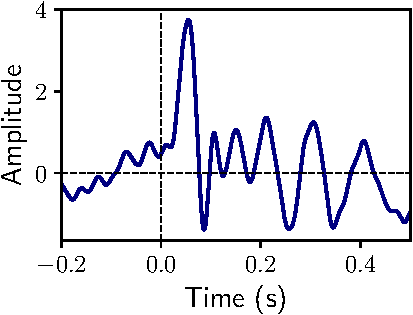
\includegraphics[width=0.3\textwidth]{figures/mvica/camcan_source_0.pdf}%
\raisebox{0.2\height}{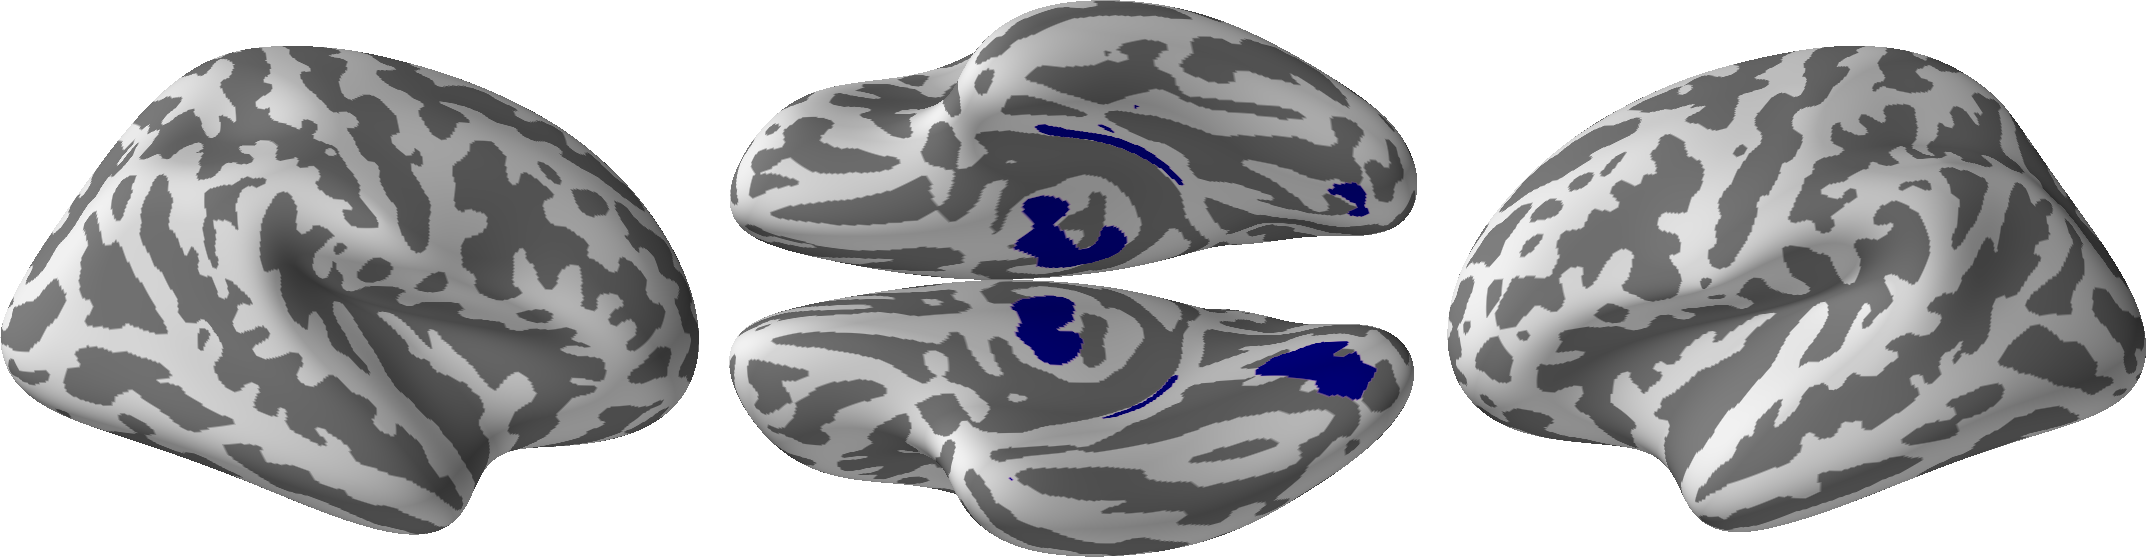
\includegraphics[width=0.68\textwidth]{figures/mvica/montage_0.png}} \\
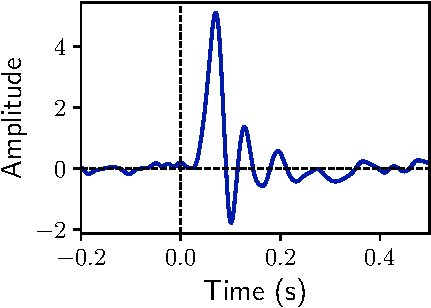
\includegraphics[width=0.3\textwidth]{figures/mvica/camcan_source_1.pdf}%
\raisebox{0.2\height}{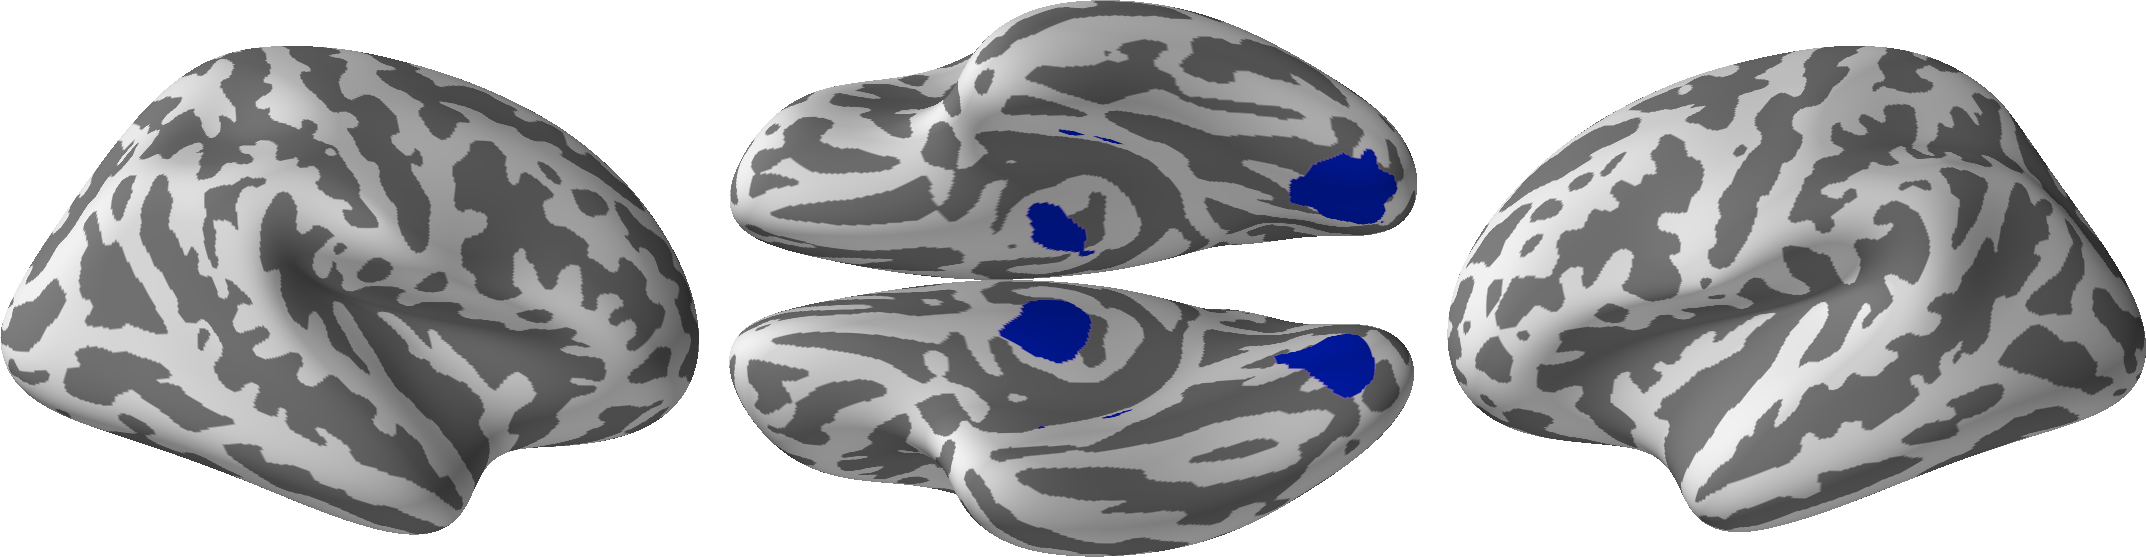
\includegraphics[width=0.68\textwidth]{figures/mvica/montage_1.png}} \\
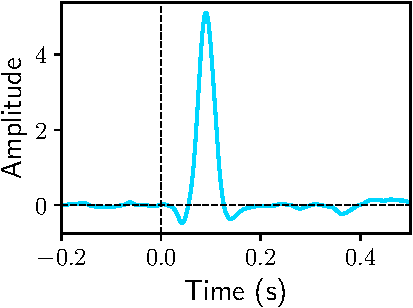
\includegraphics[width=0.3\textwidth]{figures/mvica/camcan_source_2.pdf}%                        
\raisebox{0.2\height}{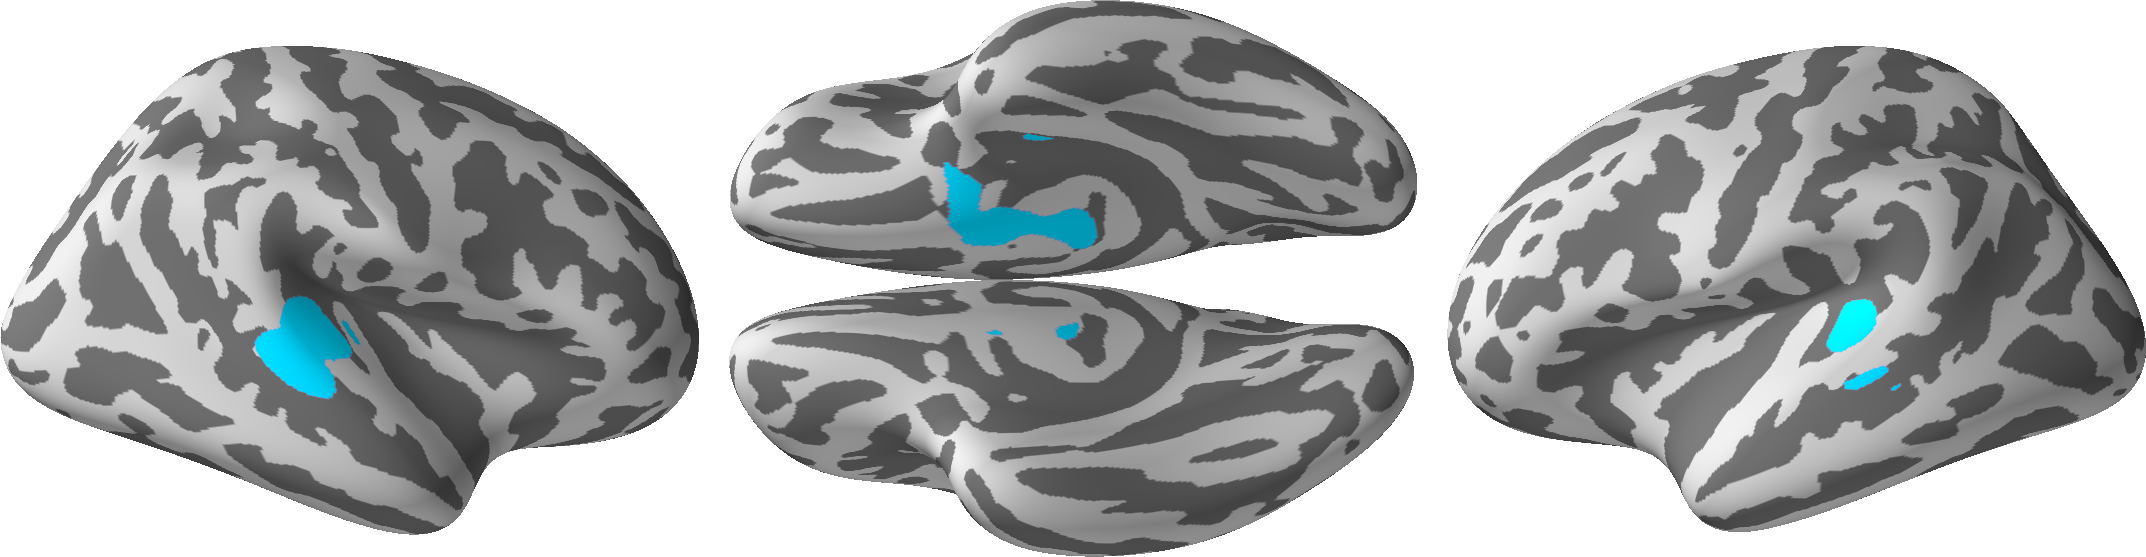
\includegraphics[width=0.68\textwidth]{figures/mvica/montage_2.png}} \\
\includegraphics[width=0.3\textwidth]{figures/mvica/camcan_source_3.pdf}%  
\raisebox{0.2\height}{\includegraphics[width=0.68\textwidth]{figures/mvica/montage_3.png}} \\
\includegraphics[width=0.3\textwidth]{figures/mvica/camcan_source_4.pdf}%
\raisebox{0.2\height}{\includegraphics[width=0.68\textwidth]{figures/mvica/montage_4.png}} \\
\includegraphics[width=0.3\textwidth]{figures/mvica/camcan_source_5.pdf}%
\raisebox{0.2\height}{\includegraphics[width=0.68\textwidth]{figures/mvica/montage_5.png}} \\
\includegraphics[width=0.3\textwidth]{figures/mvica/camcan_source_6.pdf}%
\raisebox{0.2\height}{\includegraphics[width=0.68\textwidth]{figures/mvica/montage_6.png}} \\
\includegraphics[width=0.3\textwidth]{figures/mvica/camcan_source_7.pdf}%
\raisebox{0.2\height}{\includegraphics[width=0.68\textwidth]{figures/mvica/montage_7.png}} \\
\includegraphics[width=0.3\textwidth]{figures/mvica/camcan_source_8.pdf}%
\raisebox{0.2\height}{\includegraphics[width=0.68\textwidth]{figures/mvica/montage_8.png}} \\
\includegraphics[width=0.3\textwidth]{figures/mvica/camcan_source_9.pdf}%
\raisebox{0.2\height}{\includegraphics[width=0.68\textwidth]{figures/mvica/montage_9.png}} \\
\includegraphics[width=0.3\textwidth]{figures/mvica/camcan_source_10.pdf}%
\raisebox{0.2\height}{\includegraphics[width=0.68\textwidth]{figures/mvica/montage_10.png}} \\
}

\section{Average forward operators on fMRI datasets}
\label{sec:spatial_maps}
We display the average forward operator across subjects on the Raiders, Forrest, Clips and Sherlock datasets obtained with MultiViewICA and ConcatICA with 5 components. A 5~mm spatial smoothing was applied on all datasets, and the confound signals corresponding to the 5 components with the highest variance were removed before applying MultiViewICA or ConcatICA.

{\centering

  \includegraphics[width=\textwidth]{figures/mvica/maps_forrest.png} \\
  \includegraphics[width=\textwidth]{figures/mvica/maps_sherlock.png} \\
  \includegraphics[width=\textwidth]{figures/mvica/maps_gallant.png} \\
  \includegraphics[width=\textwidth]{figures/mvica/maps_raiders.png} \\
}

\section{Synthetic benchmark using additive noise on the sensors}
\label{app:complex_cov}
We generate data according to the model $\xb_i = A_i\sbb + \nb_i$, where $\xb_i \in \mathbb{R}^{50}$, $\sbb \in \mathbb{R}^{20}$, and $\nb_i\sim \mathcal{N}(0, \sigma^2 I_{50})$. After applying individual PCA to obtain signals of dimension $20$, we apply the different ICA algorithms and report the reconstruction error in fig.~\ref{fig:reconstruction_synth}.

\begin{figure}
  \center
  \includegraphics[width=0.5\linewidth]{figures/mvica/distance.pdf}
  \caption{Synthetic experiment with model $\xb_i = A_i\sbb + \nb_i$} %{Light Unit}
  \label{fig:reconstruction_synth}
\end{figure}

\section{Summary of our quantitative results}
\label{sec:app_real_data}
Our quantitative results for the fMRI experiments of time-segment matching and BOLD signal reconstruction and on for the MEG phantom data experiment are summarized, respectively, in Table~\ref{tab:timeseg}, Table~\ref{tab:recon} and Table~\ref{tab:meg}. All methods are compared upon extraction of components with the same dimensionality ($20$ components).

\begin{table}
    \centering
    \begin{tabular}{|c|c | c | c|}
            \hline
         \textbf{Dataset} & \textbf{Method} & \textbf{Accuracy} & \textbf{Confidence interval} \\
         \hline
clips   & Chance      & 0.002&[0.001, 0.003] \\
        & CanICA    & 0.130&[0.112, 0.147] \\
        & PCA + ConcatICA      & 0.124&[0.109, 0.139] \\
        & ConcatICA    & 0.152&[0.133, 0.171] \\

        & PermICA     & 0.147&[0.126, 0.169] \\
        & SRM         & 0.115&[0.104, 0.126] \\
        & MultiViewICA& \textbf{0.167}&[0.142, 0.192] \\
        \hline
forrest & Chance      & 0.002&[0.001, 0.002] \\
        & CanICA    & 0.192&[0.170, 0.214] \\
        & PCA + ConcatICA      & 0.088&[0.077, 0.098] \\
        & ConcatICA    & 0.154&[0.137, 0.170] \\
        & PermICA     & 0.135&[0.118, 0.152] \\
        & SRM         & 0.188&[0.173, 0.203] \\
        & MultiViewICA& \textbf{0.448}&[0.411, 0.484] \\
        \hline
raiders & Chance      & 0.002&[0.001, 0.003] \\
        & CanICA    & 0.256&[0.220, 0.291] \\
        & PCA + ConcatICA      & 0.331&[0.289, 0.372] \\
        & ConcatICA    & 0.321&[0.281, 0.361] \\
        & PermICA     & 0.381&[0.341, 0.421] \\
        & SRM         & 0.265&[0.240, 0.289] \\
         & MultiViewICA& \textbf{0.408}&[0.358, 0.458] \\
         \hline
sherlock& Chance      & 0.005&[0.003, 0.006] \\
        & CanICA    & 0.607&[0.567, 0.648] \\
        & PCA + ConcatICA      & 0.454&[0.416, 0.492] \\
        & ConcatICA    & 0.519&[0.481, 0.556] \\
        & PermICA     & 0.399&[0.365, 0.434] \\
        & SRM         & 0.493&[0.465, 0.520] \\
        & MultiViewICA& \textbf{0.873}&[0.844, 0.903] \\
\hline
    \end{tabular}
    \caption{Timesegment matching: Summary of our quantitative results. We report the mean accuracy across cross-validation splits.}
    \label{tab:timeseg}
\end{table}

\begin{table}
    \centering
    \begin{tabular}{|c|c | c | c|}
            \hline
         \textbf{Dataset} & \textbf{Method} & \textbf{R2 score} & \textbf{Confidence interval} \\
         \hline
         clips   & Chance              & 0.000&[0.000 ,0.000] \\
        & CanICA            &  0.110&[ 0.097 , 0.123] \\
        & PCA + ConcatICA              &  0.075&[ 0.058 , 0.092] \\
        & ConcatICA            &  0.077&[ 0.059 , 0.094] \\
        & PermICA             &  0.099&[ 0.087 , 0.111] \\
        & SRM                 &  0.081&[ 0.069 , 0.094] \\
        & MultiViewICA        &  \textbf{0.114}&[ 0.099 , 0.128] \\
        \hline
forrest & Chance              & 0.000&[0.000 ,0.000] \\
        & CanICA            &  0.181&[ 0.169 , 0.193] \\
        & PCA + ConcatICA              &  0.072&[ 0.054 , 0.090] \\
        & ConcatICA            &  0.081&[ 0.062 , 0.099] \\
        & PermICA             &  0.098&[ 0.090 , 0.106] \\
        & SRM                 &  0.180&[ 0.168 , 0.193] \\
        & MultiViewICA        &  \textbf{0.191}&[ 0.177 , 0.204] \\
        \hline
raiders & Chance              & 0.000&[0.000 ,0.000] \\
        & CanICA            &  0.136&[ 0.122 , 0.149] \\
        & PCA + ConcatICA              &  0.063&[ 0.045 , 0.080] \\
        & ConcatICA            &  0.062&[ 0.043 , 0.081] \\
        & PermICA             &  0.107&[ 0.091 , 0.124] \\
        & SRM                 &  0.138&[ 0.121 , 0.154] \\
        & MultiViewICA        &  \textbf{0.144}&[ 0.124 , 0.164] \\
        \hline
sherlock& Chance              & 0.000&[0.000 ,0.000] \\
        & CanICA            &  0.156&[ 0.141 , 0.172] \\
        & PCA + ConcatICA              &  0.087&[ 0.065 , 0.108] \\
        & ConcatICA            &  0.091&[ 0.070 , 0.112] \\
        & PermICA             &  0.067&[ 0.055 , 0.078] \\
        & SRM                 &  \textbf{0.164}&[ 0.147 , 0.181] \\
        & MultiViewICA        &  0.161&[ 0.142 , 0.180] \\
        \hline

         
    \end{tabular}
    \caption{Reconstructing the BOLD signal of missing subjects: Summary of our quantitative results. We report the mean R2 score across cross-validation splits.}
    \label{tab:recon}
\end{table}

\begin{table}
    \centering
    \begin{tabular}{|c|c|c|c}
    \hline
         \textbf{Method} & \textbf{Reconstruction error} & \textbf{1st and 3d quartiles} 
         \\
         \hline
         MultiViewICA & \textbf{0.0045} & [0.0039, 0.0052] \\ 
ConcatICA & 0.1098 & [0.0549, 0.1734] \\ 
PCA+ConcatICA & 0.1111 & [0.0760, 0.1502] \\ 
PermICA & 0.0730 & [0.0423, 0.1037] \\ 
\hline
    \end{tabular}
    \caption{Phantom MEG data: Summary of our quantitative results with 2 epochs. We report the median reconstruction error across cross-validation splits.}
    \label{tab:meg}
\end{table}


\chapter{ShICA}
\section{Lemmas}
\label{app:sec:lemmas}
\begin{lemma}
\label{lemma:ica}
Let $\sbb \in \mathbb{R}^k$ and $\sbb'\in \mathbb{R}^k$ have independent components among which $g$ are Gaussian, and $P$ a rotation matrix such that $\sbb = P\sbb'$. Then, $P=\Pi^{-1} O \Pi'$ where $\Pi$ and $\Pi'$ are sign and permutation matrices such that the first $g$ components of $\Pi \sbb$ and $\Pi' \sbb'$ are Gaussian and $O$ is a block diagonal matrix such that $O^{(g)}$, the first $g \times g$ block of $O$, is orthogonal and the other block is identity.
\end{lemma}
\begin{proof}
  From~\cite{comon1994independent}, Theorem 10:
  Assume $\sbb = P\sbb'$, if the column $j$ of $P$ has more than one non-zero element then $s'_j$ is Gaussian. 
  
  Let us define permutations $\Pi_1$, $\Pi'_1$ such that the first $g$ components of $\Pi_1 \sbb$ and $\Pi'_1 \sbb'$ are Gaussian and $P_1  = \Pi_1 P (\Pi'_1)^{-1}$. We can see that $P_1$ is orthogonal.
  
[Omitted long matching line]
  \begin{align}
      &\begin{bmatrix} O_g & 0 \\ 0 & P_2 \end{bmatrix} = \Pi_1 P (\Pi'_1)^{-1} \\
      & \iff \begin{bmatrix} O_g & 0 \\ 0 & I \end{bmatrix} \begin{bmatrix} I & 0 \\ 0 & P_2 \end{bmatrix}  = \Pi_1 P (\Pi'_1)^{-1} \\
      & \iff \Pi_1^{-1} \begin{bmatrix} O_g & 0 \\ 0 & I \end{bmatrix} \begin{bmatrix} I & 0 \\ 0 & P_2 \end{bmatrix} \Pi'_1  = P
  \end{align}
  
  Therefore setting $\Pi' =   \begin{bmatrix} I & 0 \\ 0 & P_2 \end{bmatrix} \Pi'_1$ and $\Pi = \Pi_1$ and $O= \begin{bmatrix}O_g & 0 \\ 0 & I  \end{bmatrix}$ concludes the proof.
  
\end{proof}

\begin{lemma}
\label{lemma:eigdecomp}
Assume that Assumption 2 holds for $\Sigma_i$, and that there is an orthogonal matrix $P$ and diagonal matrices $\Sigma_i'$ such that for all $i$, $\Sigma_i' = P\Sigma_iP^{\top}$. Then, $P$ is a permutation matrix.
\end{lemma}
\begin{proof}
The proof is in two parts. First, we show that there exist some coefficients $\alpha_1, \dots, \alpha_m$ such that the matrix $\sum_i\alpha_i\Sigma_i$ has distinct coefficients on the diagonal. Then, since we have $\sum_i\alpha_i\Sigma'_i = P\left(\sum_i\alpha_i\Sigma_i\right)P^{\top}$, and the diagonal $\sum_i\alpha_i\Sigma_i$ has distinct entries, we can invoke the unicity of the eigenvalue decomposition for symmetric matrices, which shows that $P$ is necessarily a permutation matrix.
Now, the only thing left is to prove is that Assumption 2 implies the existence of this linear combination.

We assume by contradiction that any linear combination of the $\Sigma_i$ has two equal entries.

For $\alpha = [\alpha_1, \dots, \alpha_m]$, we let $\mathcal{S}(\alpha) = \diag(\sum_i\alpha_i\Sigma_i)\in\bbR^p$, where $\diag(\cdot)$ extracts the diagonal entries. The operator $\mathcal{S}$ is linear.
%
We now define for $j, j'\leq p$ the linear form $\ell_{jj'}(\alpha) = \mathcal{S}(\alpha)_j - \mathcal{S}(\alpha)_{j'}\in\bbR$. The assumption on the linear combinations of $\Sigma_i$ simply rewrites:
For all $\alpha\in\bbR^m$, there exists $j, j'\leq p$ such that $\ell_{jj'}(\alpha) = 0$.

From a set point of view, this relationship writes
$$
\bigcup_{j, j'}\mathrm{Ker}(\ell_{jj'}) = \bbR^m\enspace.
$$
Since the $\ell_{jj'}$ are all linear forms, the $\mathrm{Ker}(\ell_{jj'})$ are subspaces of dimensions $m$ or $m-1$, and since their union is of dimension $m$, there exists $j, j'$ such that  $\mathrm{Ker}(\ell_{jj'}) = \bbR^m$, i.e. such that $\ell_{jj'} = 0$.

As a consequence, we have for all $\alpha$, $\mathcal{S}(\alpha)_j = \mathcal{S}(\alpha)_{j'}$. This implies that the sequences $(\Sigma_{ij})_i$ and $(\Sigma_{ij'})_i$ are equal, which contradicts Assumption 2.


We have therefore shown that Assumption 2 implies the existence of a linear combination of the $\Sigma_i$ that has distinct entries, which concludes the proof.
\end{proof}


\begin{lemma}
\label{lemma:nonzerocoord}
Let us consider the following eigenvalue problem:
 \begin{align}
  & \begin{bmatrix} I + \Sigma_1 & I & \dots & I \\
    I & I + \Sigma_2 & \ddots & \vdots \\
    \vdots &  \ddots & \ddots & I  \\
    I & \dots & I  &I + \Sigma_m
  \end{bmatrix} \zb = \lambda \begin{bmatrix}
    I + \Sigma_1 & 0 & \dots  & 0 \\
    0 & I + \Sigma_2 & \ddots & \vdots \\
    \vdots & \ddots & \ddots & 0 \\
    0& \dots  & 0 &  I + \Sigma_m  \\
  \end{bmatrix} \zb
  \label{reducedeig}
\end{align}
where $\forall i, \enspace 1 \leq i \leq m, \enspace  \Sigma_m \in \bbR^{p, p}$ are positive diagonal matrices and I is the identity matrix.
If the first $p$ eigenvalues are distincts, the first $p$ eigenvectors $\zb^1, \dots, \zb^p, \zb^i \in \mathbb{R}^{mp}$ have different first non-zero coordinates.
\end{lemma}
%\bt{You implicitly assume that D is the block-diagonal part of C ?}
\begin{proof}
We sort the eigenvectors in $p$ groups of $m$ vectors so that all
vectors in group $l$ have their $l$-th coordinate
different from 0.
Let $\zb^{(l)}$ be an eigenvector in group $l$ and let us call $\wb_l \in
\mathbb{R}^{m}$ the non-zero coordinates of this eigenvector: $\forall i \in \{1 \dots m \}, w_{li} = z^{(l)}_{l + (i-1)p}$.

We have:
\begin{align}
\begin{bmatrix}
  1 + \Sigma_{1l} & 1 & \dots & 1  \\
  1 & 1 + \Sigma_{2l} & \ddots  &\vdots \\
  \vdots & \ddots & \ddots & 1  \\
  1 & \dots & 1 & 1 + \Sigma_{ml}  \\
\end{bmatrix} \wb_l =  \begin{bmatrix}
  1 + \Sigma_{1l} & 0 & \dots  & 0 \\
  0 & 1 + \Sigma_{2l} & \ddots & \vdots \\
  \vdots & \ddots & \ddots & 0 \\
  0& \dots  & 0 &  1 + \Sigma_{ml}  \\
\end{bmatrix} \wb_l \lambda_l
\label{eigsimp}
\end{align}

We now show that the biggest eigenvalue of~\eqref{eigsimp} is strictly above 1 while all
others are strictly below 1. The core of the proof comes from the study of the eigenvalues of a matrix modified by a rank 1 matrix. The reasoning we use here follows~\cite{golub1973some} (end of section 5).

Let us introduce 
$K^l = \diag(\Sigma_{1l} \dots \Sigma_{ml})$ and $\ub = \begin{bmatrix} 1 \\ \vdots \\ 1 \end{bmatrix}$.
Let us drop the index $l$ in the notations for simplicity.

The problem can be rewritten
\begin{align}
  &(\ub \ub^{\top} + K) \wb =  (I + K) \wb \lambda \\
  & \iff (I + K)^{-1}(\ub \ub^{\top} + K) \wb =   \wb \lambda
\end{align}

The characteristic polynomial is given by:
\begin{align}
  &\mathcal{P}(\lambda) = \det( (I + K)^{-1} K - \lambda I + (I + K)^{-1} \ub \ub^{\top}) \label{carpol} \\
  &\propto \det( I + ((I + K)^{-1} K - \lambda I)^{-1}(I + K)^{-1} \ub \ub^{\top})
\end{align}
where we implicitly focus here on eigenvalues $\lambda$ such that $\det((I + K)^{-1} K - \lambda I) \neq 0 \iff \forall i, \lambda \neq \frac{k_i}{1 + k_i}$.

We then use the following property:
Let $A \in \mathbb{R}^{a, b}$ and $B \in \mathbb{R}^{b, a}$ we have
$\det(I_a + AB) = \det(I_b + BA)$.

Let us call $\chi(\lambda) = \det( I + ((I + K)^{-1} K - \lambda I)^{-1}(I + K)^{-1} \ub \ub^{\top})$ we have:
\begin{align}
\chi(\lambda)
  &= 1 + \ub^{\top}((I + K)^{-1} K - \lambda I)^{-1}(I + K)^{-1} \ub \\
  &= 1  + \sum_{i=1}^m \frac1{1 + k_i} \frac1{ \frac{k_i}{1 + k_i} - \lambda}
\end{align}
%\bt{transition from (16) to (17) is not obvious to me !}
where $k_i = \Sigma_{il} > 0$.
% Since $k_i = \Sigma_{il} > 0$, the above secular function is simple to
% study.
% Let us re-order the values $\kappa_i = \frac{k_i}{1 + k_i}$ by increasing
% order $\kappa_1 < \dots < \kappa_m$. The eigenvalues $\lambda_i$ are such that
% $\kappa_1 < \lambda_1 < \kappa_2 < \lambda_2 < \kappa_3 < \dots < \kappa_m <
% \lambda_m$.
% Trivially $\kappa_m < 1$.
Taking the derivative we get 
\begin{align}
\chi'(\lambda) = \sum_{i=1}^m \frac1{1 + k_i} \frac1{ (\frac{k_i}{1 + k_i} - \lambda)^2} > 0
\end{align}

Trivially, $\forall i, \frac{k_i}{1 + k_i} < 1$. We also have
\begin{align}
  \chi(1) = 1 + \sum_{i=1}^{m} \frac1{1 + k_i} \frac1{ \frac{k_i}{1 + k_i} - 1} = 1 - m < 0
\end{align}
 and $\lim_{\lambda \rightarrow + \infty} \chi(\lambda) = 1$ so as $\chi$
 is continuous and strictly increasing on $[1, +\infty[$. Therefore, it reaches $0$ only once on this interval (excluding 1 since we know $\chi(1) \neq 0$). Therefore the greatest eigenvalue $\lambda^*$ is strictly above $1$ while all other eigenvalues are strictly below $1$.
 
  Note that because $\chi' > 0$, $\lambda^*$ is of multiplicity $1$. In the analysis above we ignored those eigenvalues $\lambda$ such that $\lambda = \frac{k_i}{1 + k_i}$ for some $i$. However since $\frac{k_i}{1 + k_i} < 1$, none of these eigenvalues can be the largest one.
 
 Finally, the $p$ first eigenvectors belong to different groups (the
 corresponding eigenvalues are all strictly above 1). This shows that these eigenvectors have
 different first non-zero coordinates. 
 
\end{proof}

% \begin{lemma}
% \label{lemma:rotation}
%   Let us consider the problem $(\Lambda + \delta
%   E)\ub = \ub \psi$ where $\Lambda = \diag(\lambda_1 \dots \lambda_{mp})$ is a diagonal matrix of positive values arranged in decreasing order, $\delta E = o(\lambda_p - \lambda_{p+1})$ and $\delta E = o(\lambda_{pm})$. The first eigenvectors $[\ub^1 \dots  \ub^p]$ are given by
%   $[\ub^1 \dots \ub^p] = [e_1 \dots e_p] \Theta + \delta Z$ where $e_i$ are the vectors of the canonical basis in $\bbR^{mp}$,
%   $\Theta \in \mathbb{R}^{p \times p}$ is a rotation matrix and $\delta Z =
%   O(\delta E)$
% \end{lemma}
% \begin{proof}
%   In matrix form denoting $\Psi = \diag(\psi_1 \dots \psi_{mp})$ the eigenvalues
%   in descending order and $U = [\ub^1 \dots \ub^{mp}]$ the matrix of associated
%   eigenvectors.
%   We want to solve
%   \begin{align}
%     (\Lambda +  \delta E)  U =  U \Psi
%   \end{align}
%   When the difference between any two values of $\Lambda$ is in $O(\min(\lambda_{pm}, \lambda_p - \lambda_{p+1}))$, no
%   rotation indeterminacy appears. We refer the reader to section 3.1 of the tutorial of~\cite{bamieh2020tutorial} to
%   have an explicit formula:
%   $U = I - \Pi \odot \delta E$
%   where $\odot$  is the Hadamar product and
%   $\Pi_{ij} = \begin{cases}
%     0 & \text{if } i =j \\
%     \frac1{\lambda_i - \lambda_j} & \text{if } i \neq i \\
%   \end{cases}$.

%   The rotation indeterminacy appears whenever the difference between two values
%   in $\Lambda$ is of the same order than $\delta E$. In which case we can
%   reparametrize the problem by:
%   \begin{align}
%     (\Lambda' +  \delta E')  U =  U \Psi
%   \end{align}
%   where $\Lambda'$ is obtained by replacing $\lambda_i$ by $\lambda_{i-1}$
%   whenever $\lambda_i - \lambda_{i-1} = O(\delta E)$ and the corresponding terms are
%   added in $\delta E'$ so that we always have $\Lambda + \delta E = \Lambda' +
%   \delta E'$ and $\delta E' = O(\delta E)$.

%   Let us assume without loss of generality that the $l$ first diagonal values of
%   $\Lambda'$ are the same while all others are different. Following derivations in~\cite{bamieh2020tutorial}, the
%   eigenvectors are given by:
%   \begin{align}
%     U = \Theta - \Theta \Pi' \odot \Theta^{\top}\delta E' \Theta
%   \end{align}
%   where $\Theta$ is a matrix such that its first $l, l$ block $\Theta^l$ diagonalizes the
%   first $l, l$ block of $\delta E'$, the off-diagonal blocks are nul and the
%   last diagonal block is identity.
%   \[
%     \Theta = \begin{bmatrix} \Theta^l & 0 \\ 0 & I_{km - l} \\ \end{bmatrix}
%   \]
%   and $\Pi'$ is given by
%   $\Pi'_{ij} = \begin{cases} 0 & \text{if } \lambda_i = \lambda_j \\
%     \frac1{\lambda_i - \lambda_j} & \text{if } \lambda_i \neq \lambda_j
%   \end{cases}$.
  
%   This can be rewritten:
%   \begin{align}
%       [\ub^1 \dots \ub^l] = [\eb_1 \dots \eb_l]\Theta^l
%       [\ub^{l+1} \dots \ub^{pm}] = [\eb_{l+1} \dots \eb_{pm}]
%   \end{align}
%   In particular we see that the eigenvectors are given up to a correction term by the canonical vectors with eigenvalues given (up to a correction term) by the diagonal values in $\Lambda$, but the ones that correspond to the same values of $\lambda_i$ up to $O(\delta_E)$ undergo a rotation $\Theta^l$ that depends on the sampling noise.
  
%   Note that as $\delta E = o(\lambda_p - \lambda_{p+1})$, none of the first $p$ eigenvectors can have the same eigenvalue as the last $pm -p$ up to $O(\delta E)$.
%   Therefore the first $p$ eigenvectors are given by the first $p$ canonical vectors of $\bbR^{pm}$ up to a rotation and a correction term: $[\ub^1 \dots \ub^p] = [e_1 \dots e_p]
%   \mathcal{O} + \delta Z$. Where $\mathcal{O} \in \bbR^{p, p}$ is a rotation and $\delta Z = O(\|\delta E \|_F^2)$.
% \end{proof}
% \bt{I'm lost between $\Theta$ and$ \mathcal{O}$}

\section{Identifiability results for $m< 3$}
\label{app:identifiability}
We have a slightly weaker identifiability result when $m=2$.
\begin{proposition}
  \label{prop:identifiability_2d}
  Let $m=2$, and suppose that the scalars $(1 + \Sigma_{1j})(1+\Sigma_{2j})$ for $j=1\dots p$ are all different. We let $\Theta'=(A_1', A_2', \Sigma_1',\Sigma_2')$ that also generates $\xb_1, \xb_2$. Then, there exists a permutation and scale matrix $P$ such that $A'_1 =A_1P$ and $A'_2 = A_2P^{-\top}$.
\end{proposition}
\begin{proof}
  We let $P=A_1^{-1}A_1'$. Since $C_{12} = I_p$, it holds 
  $A_2^{-1}A_2'= P^{-\top}$. Then, we have
  $I_p + \Sigma_1 = P(I_p + \Sigma'_1)P^{\top}$. This means that there exists $U\in\mathcal{O}_p$ such that $P = (I_p + \Sigma_1)^{\frac12}U(I_p + \Sigma'_1)^{-\frac12}$. Since $P^{-\top}(I_p+\Sigma'_2)P^{-1} = I_p+\Sigma_2$, we find
  $U(I_p+\Sigma'_1)(I_p+\Sigma'_2)U^{\top} = (I_p+\Sigma_1)(I_p+\Sigma_2)$. By identification, $U$ is a permutation matrix, and $P$ is a scale and permutation matrix.
\end{proof}
As a consequence, when there are only two subjects, it is possible to recover the components and noise levels up to a scaling factor.
%
When there is only one view, $m=1$, there is a global rotation indeterminacy: 
$
A_1(I_p + \Sigma_1)A_1^{\top} = A'_1(I_p + \Sigma_1){A'_1}^{\top}
$
for $A'_1 = A_1(I_p + \Sigma_1)^{\frac12}U(I_p + \Sigma_1)^{-\frac12}$ where $U$ is any orthogonal matrix. In this case, we lose identifiability.

% \section{Derivation of gradient and Hessian for the joint diagonalization}
% \label{app:jointdiag}
% We use a similar approach as\pierre{do we really need the orthogonal algorithm ? anyways, this should be put in appendix} in~\cite{ablin2018beyond} and optimize this loss using a quasi-newton approach. In our case though, we have to take into account the orthogonality constraint.
% In order to take into account orthogonality constraints, the gradient $G$ and Hessian $H$ are defined as 
% $\loss(\exp(\eps) O) = \loss(O) + \dotp{ \eps }{ G } + \dotp{ \eps }{ H \eps } + o(\|\eps \|_F^2)$ where $\eps$ is a small skew-symmetric matrix.

% Let us call $D^i = \mathcal{O} \hat{W}_i C_{ii} \hat{W}_i^{\top} \mathcal{O}^{\top}$ and notice that $D^i$ is symmetric.
% We have
% \begin{align}
%     &\loss(\exp(\eps) \mathcal{O}) \\
%     &= \loss((I + \eps + \frac12 \eps^2) \mathcal{O}) + o(\|\eps^2\|) \\
%     &= \frac1{2n} \sum_{i=1}^m \log \det \diag((I + \eps + \frac12 \eps^2) D^i(I + \eps + \frac12 \eps^2)^{\top}) + o(\|\eps^2\|) \\
%     &= \frac1{2n} \sum_{i=1}^m \log \det( \diag(D^i) + \diag(D^i \eps^{\top}) + \diag(\eps D^i) + \\ &\enspace \enspace \enspace \enspace \diag(\eps D^i \eps^{\top}) + \diag(\frac12 \eps^2 D^i) + \diag(\frac12 D^i (\eps^2)^{\top})) + o(\|\eps^2\|)\\
%     &= \frac1{2n} \sum_{i=1}^m \log \det( \diag(D^i) + 2\diag(\eps D^i) + \diag(\eps D^i \eps^{\top}) + 2\diag(\frac12 \eps^2 D^i)) + o(\|\eps^2\|)\\
%     &= \loss(\mathcal{O}) + \frac1{2n} \sum_{i=1}^m \log \det( I + 2\frac{\diag(\eps D^i)}{\diag(D^i)} + \frac{\diag(\eps D^i \eps^{\top})}{\diag(D^i)} + 2\frac{\diag(\frac12 \eps^2 D^i)}{\diag(D^i)}) + o(\|\eps^2\|) \\
%     &= \loss(\mathcal{O}) + \frac1{2n} \sum_{i=1}^m \tr \log( I + 2\frac{\diag(\eps D^i)}{\diag(D^i)} + \frac{\diag(\eps D^i \eps^{\top})}{\diag(D^i)} + 2\frac{\diag(\frac12 \eps^2 D^i)}{\diag(D^i)}) + o(\|\eps^2\|) \\
%     &= \loss(\mathcal{O}) + \frac1{2n} \sum_{i=1}^m \tr( 2\frac{\diag(\eps D^i)}{\diag(D^i)} + \frac{\diag(\eps D^i \eps^{\top})}{\diag(D^i)} \\ &\enspace \enspace \enspace \enspace + 2\frac{\diag(\frac12 \eps^2 D^i)}{\diag(D^i)} - 2(\frac{\diag(\eps D^i)}{\diag(D^i)})^2) + o(\|\eps^2\|) \\
%     &= \loss(\mathcal{O}) + \frac1{2n} \sum_{i=1}^m  \sum_k \left[ \sum_l 2\frac{\eps_{kl} D^i_{lk}}{D^i_{kk}} + \sum_{lm} \frac{\eps_{kl} D^i_{lm} \eps_{km}}{D^i_{kk}} \right.\\  &\left.\enspace \enspace \enspace \enspace + \sum_{lm}\frac{ \eps_{kl} \eps_{lm} D^i_{mk}}{D^i_{kk}} - 2\sum_{lm} \frac{ \eps_{kl}D^i_{lk} \eps_{km}D^i_{mk}}{(D^i_{kk})^2} \right] + o(\|\eps^2\|)
% \end{align}
% By identification we get
% \begin{align}
%     &G_{kl} = \frac1{n} \sum_i \frac{D^i_{lk}}{D^i_{kk}}
%     &H_{klmn} = \frac1{n} \sum_i (\delta_{km} \frac{D^i_{ln}}{D^i_{kk}} + \delta_{lm}\frac{D^i_{nk}}{D^i_{kk}} - 2 \delta_{km} \frac{D^i_{lk} D^i_{nk}}{(D^i_{kk})^2})
% \end{align}

% \begin{align}
%     &G_{kl} = \frac1{n} \sum_i \frac{D^i_{lk}}{D^i_{kk}}
%     &H_{klmn} = \frac1{n} \sum_i (\delta_{km} \frac{D^i_{ln}}{D^i_{kk}} + \delta_{lm}\frac{D^i_{nk}}{D^i_{kk}} - 2 \delta_{km} \frac{D^i_{lk} D^i_{nk}}{(D^i_{kk})^2})
% \end{align}
% We approximate the Hessian by replacing $D^i_{lk}$ by $D^i_{kk} \delta_{lk}$. This approximation is exact when the unmixed covariances are truly diagonal. The approximated Hessian is given by
% $\hat{H}_{klmn} = \frac1{n} \sum_i (\delta_{km} \delta_{ln} \frac{D^i_{ll}}{D^i_{kk}} + \delta_{lm} \delta_{kn} - 2 \delta_{kmln})$.
% Using the fact that $\eps$ is a skew-symmetric matrix

% Let us call $\hat{D^i} = \frac1{n} \sum_i D^i$.
% \begin{align}
% \dotp{ G }{ \eps } + \frac12 \dotp{ \eps }{ \hat{H} \eps } &= \sum_{kl} \eps_{kl} G_{kl} + \frac12 \sum_{klmn} \hat{H}_{klmn} \eps_{kl} \eps_{mn} \\
% &= \sum_{kl} G_{kl} \eps_{kl} + \frac12 \left[\sum_{kl} \frac{\hat{D}^i_{ll}}{\hat{D}^i_{kk}} \eps_{kl}^2 + \sum_{kl}\eps_{kl} \eps_{lk} - 2\sum_k \eps_{kk} \right]
% \end{align}
% Using the fact that $\eps$ is anti-symmetric gives:
% \begin{align}
% \dotp{ G }{ \eps } + \dotp{ \eps }{ \hat{H} \eps }
% &= \sum_{k} \sum_{l < k} (G_{kl} - G_{lk}) \eps_{kl} + \frac12(\sum_{k} \sum_{l < k} (\frac{\hat{D}^i_{ll}}{\hat{D}^i_{kk}} + \frac{\hat{D}^i_{kk}}{\hat{D}^i_{ll}}) \eps_{kl}^2 -\sum_{k} \sum_{l < k}2\eps_{kl}^2) \\
% &= \sum_{k} \sum_{l < k} (G_{kl} - G_{lk}) \eps_{kl} + \frac12(\sum_{k} \sum_{l < k} \left[\frac{\hat{D}^i_{ll}}{\hat{D}^i_{kk}} + \frac{\hat{D}^i_{kk}}{\hat{D}^i_{ll}} - 2\right] \eps_{kl}^2)
% \end{align}
% So updates are given by
% $\mathcal{O} \leftarrow \exp(J) \mathcal{O}$ where $J_{kl} = \frac{G_{kl} - G_{lk}}{\frac{\hat{D}^i_{ll}}{\hat{D}^i_{kk}} + \frac{\hat{D}^i_{kk}}{\hat{D}^i_{ll}} - 2}$.


% \section{Derivation of log-likelihood}
% \label{likelihood_derivation}


% and the log-likelihood writes:
% \begin{align}
%   \mathcal{L} = &\sum_{i=1}^m\left(-\log|W_i| + \frac12 \log |\Sigma_i|\right) + \frac12 \log(|\sum_{i=1}^m \Sigma_i^{-1} + I|) + \frac12 (\sum_{i=1}^m \dotp{ \yb_i }{ \Sigma_i^{-1} \yb_i } \\&  - \frac12 \dotp{ \left(\sum_{i=1}^m \Sigma_i^{-1} + I \right)^{-1} \sum_{i=1}^m \left(\Sigma_i^{-1} \yb_i \right) }{ \sum_{i=1}^m \left(\Sigma_i^{-1} \yb_i \right) })
% \end{align}
% which yields the expected formula.

\section{EM E-step and M-step for ShICA with Gaussian components}
  \subsection{E-step}
  \label{conditional_density}
  The derivations are the same as in section~\ref{app:emestep1} but the sum over
  $\alpha \in {\frac12, \frac32}$ is replaced by just $\alpha=1$.


\subsection{M-step}
The function to minimize in the M-step is then given by:
\begin{align}
  \Jcal &= -\log p(\xb, \sbb) \\
        &= \sum_{i=1}^m \log(|\Sigma_i|) + \\ &\enspace \enspace \enspace \frac12 \tr(\Sigma_i^{-1} \left[(\yb_i - \EE[\sbb | \xb]) (\yb_i - \EE[\sbb | \xb])^{\top}+ \VV[\sbb | \xb]\right]) \\ &\enspace \enspace \enspace + c
\end{align}
where $c$ does not depend on $\Sigma_i$

Therefore we get closed-form updates for $\Sigma_i$: 
\begin{align}
\Sigma_i \leftarrow  \diag((\yb_i - \EE[\sbb | \xb]) (\yb_i - \EE[\sbb | \xb])^{\top}+ \VV[\sbb | \xb])
\end{align}
Plugging in the closed-form formula for $\EE[\sbb|\xb]$ and $\VV[\sbb|\xb]$ we get updates that only depends on the covariances $\hat{C_{ij}} = \EE[\xb_i \xb_j^{\top}]$.
\begin{align*}
\Sigma_i \leftarrow &\diag(\hat{C_{ii}} \\&- 2 \VV[\sbb | \xb]  \sum_{j=1}^m \Sigma_j^{-1} \hat{C}_{ji}  \\&+ \VV[\sbb | \xb]  \sum_{j = 1}^m \sum_{l = 1}^m \left(\Sigma_j^{-1} \hat{C}_{jl} \Sigma_l^{-1} \right) \VV[\sbb | \xb] \\&+ \VV[\sbb | \xb])
\end{align*}


\section{EM E-step and M-step for ShICA with non-Gaussian components}
\label{app:emestep}

  \subsection{E-step}
  \label{app:emestep1}
  The complete likelihood is given by
\begin{align}
  p(\xb, \sbb) &= \prod_i p(\xb_i | \sbb) p(\sbb) \\
  &= \prod_i p(\xb_i | \sbb) \prod_j \sum_{\alpha \in \{0.5, 1.5\}}p(s_j | \alpha) \\
\end{align}
where 
\begin{align}
  p(s_j | \alpha) = \Ncal(s_j; 0, \alpha)
\end{align}

We have
\begin{align}
  p(\xb_i | \sbb) &=|W_i|\Ncal(\yb_i; \sbb, \Sigma_i)  \\
                  &= |W_i| \prod_j \Ncal(y_{ij}; s_j, \Sigma_{ij})
\end{align}
where $\Sigma_{ij}$ is the coefficient $j, j$ of $\Sigma_i$ and $\yb_i = W \xb_i$.

Let us introduce a first lemma:
\begin{lemma}
  \label{lemma:multmgauss}
  \begin{align*}
    \prod_{i=1}^m \Ncal(x_i; u, v_i) = \prod_{i=1}^m \Ncal(x_i; \bar{x}, v_i) \sqrt{2 \pi \bar{v}} \Ncal(\bar{x}; u, \bar{v})
  \end{align*}
  where $\bar{v} = (\sum_{i=1}^m v_i^{-1})^{-1}$ and $\bar{x} = \frac{\sum_i v_i^{-1}
    x_i}{\sum_i v_i^{-1}}$.
\end{lemma}
\begin{proof}
  We have that
  \begin{align}
    \frac1{v_i}(x_i - u)^2 &= \frac1{v_i}(x_i - u)^2 \\
                           &=\frac1{v_i}(x_i - \bar{x} + \bar{x} - u)^2 \\
                           &=\frac1{v_i}(x_i - \bar{x})^2 + \frac1{v_i}(\bar{x} - u)^2 \label{eq:lem:multigauss}
  \end{align}
  and therefore
  \begin{align}
    &\prod_i \frac1{\sqrt{2 \pi v_i}}\exp(-\frac1{2v_i}(x_i - \mu)^2) \\
    &= \prod_j \frac1{\sqrt{2 \pi v_i}}\exp(-\frac12 (\frac1{v_i}(x_i - \bar{x})^2 + \frac1{v_i}(\bar{x} - u)^2)) \\ 
    &= \prod_j \Ncal(x_i, \bar{x}, v_i) \exp(-\frac12( \sum_i \frac1{v_i})(\bar{x} - u)^2)) \\ 
  \end{align}
    so the desired result follow.
\end{proof}

By Lemma~\ref{lemma:multmgauss}, we have
\begin{align}
  \prod_i p(\xb_i | \sbb) &= \prod_i |W_i| \prod_j \Ncal(y_{ij}; \bar{y}_{j}, \Sigma_{ij}) \sqrt{2 \pi \bar{\Sigma_{j}}} \Ncal(\bar{y}_j; s_j, \bar{\Sigma_{j}})  \\
\end{align}
where $\bar{y}_j = \frac{\sum_i \Sigma_{ij}^{-1} y_{ij}}{ \sum_i
  \Sigma_{ij}^{-1}}$ and $\bar{\Sigma_{j}} = (\sum_i
\Sigma_{ij}^{-1})^{-1}$.
Hiding variable that do not depend on $\sbb$ we obtain

\begin{align}
  \prod_i p(\xb_i | \sbb) &\propto \prod_j \Ncal(\bar{y}_j; s_j, \bar{\Sigma_{j}})  \\
\end{align}

Then we get
\begin{align}
  p(\xb, \sbb) &= \prod_j \sum_{\alpha \in \{0.5, 1.5\}} \Ncal(s_j; \bar{y}_j, \bar{\Sigma_{j}}) \Ncal(s_j; 0, \alpha)
\end{align}

Let us now prove a second Lemma:
\begin{lemma}
  \label{lemma:multgauss}
  \begin{align*}
    \mathcal{N}(x; y, \nu) \mathcal{N}(x, 0, \alpha) = \mathcal{N}(y; 0, \nu + \alpha) \mathcal{N}(x; \frac{\alpha y}{\alpha + \nu}, \frac{\nu \alpha}{\alpha + \nu})
  \end{align*}
\end{lemma}
\begin{proof}

  We have 
\begin{align}
  &\mathcal{N}(x; y, \nu) \mathcal{N}(x, 0, \alpha) = \frac{\exp \left(-\frac{(x-y)^2}{2\nu} \right)}{\sqrt{2 \pi \nu}} \frac{\exp \left(-\frac{x^2}{2\alpha}\right)}{\sqrt{2 \pi \alpha}}
\end{align}

Then,
\begin{align}
  &\exp \left(-\frac{(x-y)^2}{2\nu} \right) \\
  &= \exp\left(- \frac{\alpha (x-y)^2 + \nu x^2}{2 \alpha \nu} \right) \\
  &= \exp\left(- \frac{\alpha (x^2 -2xy + y^2) + \nu x^2}{2 \alpha \nu} \right) \\ 
  &=\exp\left(- \frac{x^2(\alpha + \nu) -2x(\alpha y) + \alpha y^2 }{2 \alpha \nu} \right) \\
  &= \exp\left( -\frac{x^2 -2x\frac{\alpha y}{\alpha + \nu} + \frac{\alpha y^2}{\alpha + \nu} }{2 \frac{\alpha \nu}{\alpha + \nu}} \right) \\
  &= \exp\left( -\frac{(x - \frac{\alpha y}{\alpha + \nu})^2 - ( \frac{\alpha y}{\alpha + \nu} )^2 + \frac{\alpha y^2}{\alpha + \nu} }{2 \frac{\alpha \nu}{\alpha + \nu}} \right) \\
  &= \exp\left( -\frac{(x - \frac{\alpha y}{\alpha + \nu})^2}{2\frac{\alpha \nu}{\alpha + \nu}}\right) \exp \left(-\frac{ - \alpha^2 y^2 + (\alpha + \nu)\alpha y^2 }{2 \alpha \nu(\alpha + \nu)} \right) \\
  &= \exp\left( -\frac{(x - \frac{\alpha y}{\alpha + \nu})^2}{2\frac{\alpha \nu}{\alpha + \nu}}\right) \exp \left(-\frac{\nu\alpha y^2 }{2 \alpha \nu(\alpha + \nu)} \right)
\end{align}

and
\begin{align}
  \frac1{\sqrt{2 \pi \nu}\sqrt{2 \pi \alpha}} &= \frac1{\sqrt{2 \pi (\nu + \alpha)}\sqrt{2 \pi \frac{\nu \alpha}{\nu + \alpha}}}
\end{align}
so that the desired result follow.
\end{proof}
                 
By Lemma~\ref{lemma:multgauss}, we have:
\begin{align}
  &p(\xb, \sbb) \\
  &= \prod_j \sum_{\alpha \in \{0.5, 1.5\}} \Ncal(\bar{y}_{j}; 0 , \bar{\Sigma}_{j} + \alpha) \Ncal(s_j; \frac{\alpha \bar{y}_{j}}{\alpha + \bar{\Sigma_{j}}}, \frac{\bar{\Sigma_{j}}\alpha}{\alpha + \bar{\Sigma_{j}}})
\end{align}

and therefore we get:
\begin{align}
  p(\sbb | \xb) &= \frac{p(\sbb, \xb)}{\int_{\sbb} p(\sbb, \xb)} \\
                &= \prod_j \frac{\sum_{\alpha \in \{0.5, 1.5\}} \theta_{\alpha} \Ncal(s_j; \frac{\alpha \bar{y}_{j}}{\alpha + \bar{\Sigma_{j}}}, \frac{\bar{\Sigma_{j}}\alpha}{\alpha + \bar{\Sigma_{j}}})}{\sum_{\alpha \in \{0.5, 1.5\}} \theta_{\alpha}}
\end{align}
where $\theta_{\alpha} = \Ncal(\bar{y}_{j}; 0 , \bar{\Sigma}_{j} + \alpha)$.

So we obtain the desired result:
\begin{align}
  &\EE[s_j | \xb] = \frac{\sum_{\alpha \in \{0.5, 1.5\}} \theta_{\alpha} \frac{\alpha \bar{y}_{j}}{\alpha + \bar{\Sigma_{j}}}}{\sum_{\alpha \in \{0.5, 1.5\}} \theta_{\alpha}} \\
  & \VV[s_j | \xb] = \frac{\sum_{\alpha \in \{0.5, 1.5\}} \theta_{\alpha} \frac{\bar{\Sigma_{j}}\alpha}{\alpha + \bar{\Sigma_{j}}}}{\sum_{\alpha \in \{0.5, 1.5\}} \theta_{\alpha}}  
\end{align}

\subsection{M-step}
The function to minimize in the M-step is then given by:
\begin{align}
  \Jcal &= -\log p(\xb, \sbb) \\
  &= \sum_{i=1}^m - \log(|W_i|) + \log(|\Sigma_i|) + \\& \enspace \enspace \frac12 \tr(\Sigma_i^{-1} \left[(\yb_i - \EE[\sbb | \xb]) (\yb_i - \EE[\sbb | \xb])^{\top}+ \VV[\sbb | \xb]\right]) + c
\end{align}
where $c$ does not depend on $\Sigma_i$ or $W_i$

Therefore we get closed-form updates for $\Sigma_i$: 
\begin{align}
\Sigma_i \leftarrow  \diag((\yb_i - \EE[\sbb | \xb]) (\yb_i - \EE[\sbb | \xb])^{\top}+ \VV[\sbb | \xb])
\end{align}

% and the approximated Hessian $\widehat{\mathcal{H}^{W_i}}$
We update $W_i$ by performing a quasi-Newton step. 
% The gradient $\mathcal{G}^{W_i}$, the Hessian $\mathcal{H}^{W_i}$  are given by
% $\mathcal{G}((I + \epsilon)W_i) = C(W_i) + \dotp{ \epsilon }{ \mathcal{G}^{W_i} } +
% \frac12 \dotp{ \epsilon }{ \mathcal{H}^{W_i} \epsilon }$ so
% \begin{align*}
%   &\mathcal{G}^{} = -I + (\Sigma_i)^{-1}(\yb_i - \mathbb{E}[\sbb|\xb])(\yb_i)^{\top} , \enspace \mathcal{H}^{W_i}_{a, b, c, d} = \delta_{a, c} \frac{y_{ib} y_{id}}{\Sigma_i_a}, \enspace \widehat{\mathcal{H}^{W_i}_{a, b, c, d}} =  \delta_{a, c} \delta_{b, d}\frac{(y_{ib})^2}{\Sigma_i_a}
% \end{align*}
% where the Hessian approximation is exact when the unmixed data have truly independent components.

We use the relative gradient $\mathcal{G}^{W_i}$ and $\mathcal{H}^{W_i}$ defined
by
\begin{align}
\mathcal{J}(W_i + \varepsilon W_i) = \mathcal{J}(W_i) + \dotp{ \varepsilon}{\mathcal{G}^{W_i}} + \frac12 \dotp{ \varepsilon}{\mathcal{H}^{W_i} \varepsilon }
\end{align}

 We get:
 \begin{align}
   \mathcal{J}(W_i + \varepsilon W_i) &= \sum_{i=1}^m \bigg[ -\log(|W_i|) -\log(|I_k + \varepsilon|) \nonumber \\&- \log(\mathcal{N}(\yb_i + \varepsilon \yb_i; \sbb; \Sigma_i)) \bigg] + const \\
                                      &= \mathcal{J}(W_i) - \tr(\varepsilon) + \frac12 \tr(\varepsilon^2) \nonumber \\& \enspace \enspace + \frac12 \bigg[\dotp{ \varepsilon \yb_i}{ (\Sigma_i)^{-1} (\yb_i - \sbb) } + \nonumber \\& \enspace \enspace \dotp{ (\yb_i - \sbb)}{ (\Sigma_i)^{-1} \varepsilon \yb_i } + \dotp{ \varepsilon \yb_i}{ (\Sigma_i)^{-1} \varepsilon \yb_i } \bigg] \nonumber \\ & \enspace + o(\|\varepsilon\|^2) \\
                                      &= \mathcal{J}(W_i) - \sum_a \varepsilon_{a, a} + \frac12 \sum_{a, b} \varepsilon_{a,b} \varepsilon_{b, a} \nonumber \\& \enspace \enspace + \sum_{a, b} \varepsilon_{a, b} \left[(\Sigma_i)^{-1}(\yb_i - \sbb) (\yb_i)^{\top} \right]_{a, b} \nonumber \\& \enspace \enspace + \frac12 \sum_{a, b} \varepsilon_{a, b} \left[(\Sigma_i)^{-1} \varepsilon \yb_i (\yb_i)^{\top}\right]_{a, b} \nonumber \\ & \enspace + o(\|\varepsilon\|^2) \\
                                      &= \mathcal{J}(W_i) - \sum_a \varepsilon_{a, a} + \frac12 \sum_{a, b} \varepsilon_{a,b} \varepsilon_{b, a} \nonumber \\& \enspace \enspace + \sum_{a, b} \varepsilon_{a, b} \left[(\Sigma_i)^{-1}(\yb_i - \sbb) (\yb_i)^{\top} \right]_{a, b} + \nonumber \\& \enspace \enspace \frac12 \sum_{a, b, d} \varepsilon_{a, b} (\Sigma_i)^{-1}_{a, a} \varepsilon_{a, d} \left[\yb_i (\yb_i)^{\top}\right]_{d, b} \nonumber \\ & \enspace + o(\|\varepsilon\|^2)
 \end{align}

 So:
 \begin{equation}
 \mathcal{G}^{W_i}_{a, b} =  -\delta_{a,b} + \left[(\Sigma_i)^{-1} (\yb_i - \sbb)(\yb_i)^{\top}\right]_{a, b}
 \end{equation}
 and
 \begin{equation}
 \mathcal{H}^{W_i}_{a, b, c, d} = \delta_{a, d}\delta_{b, c} + \delta_{a, c} \frac{y_{ib} y_{id}}{\Sigma_{ia}}
 \end{equation}
 
 We approximate the Hessian by
 \begin{align}
 \widehat{\mathcal{H}^{W_i}_{a, b, c, d}} = \delta_{ad} \delta_{bc} + \delta_{ac} \delta_{bd}\frac{(y_{ib})^2}{\Sigma_{ia}}
\end{align}
where the Hessian approximation is exact when the unmixed data have truly independent components.

Updates for $W_i$ are then given by
$W_i \leftarrow (I - \rho (\widehat{\mathcal{H}^{W_i}})^{-1} \mathcal{G}^{W_i}) W_i$, 
where $\rho$ is chosen by backtracking line-search.
We alternate between computing the statistics $\mathbb{E}[\sbb|\xb]$ and
$\Var[\sbb|\xb]$ (E-step) and updates of parameters $\Sigma_i$ and $W_i$ for $i=1 \dots m$ (M-step).




% \begin{figure}
%   \includegraphics[width=0.5\textwidth]{./figures/synthetic_Gaussian_source_50_samples.pdf}
% \end{figure}

\section{CamCAN spatial maps}
\label{app:shica:maps}
We use $m=496$ subjects and fit ShICA-ML with $p=10$ components. We localize the
components of each subject using sLORETA~\cite{pascual2002standardized}. Then
components are registered to a common brain and averaged. Thresholded maps are
displayed below along with the time courses of each component. Spatial maps obtained with ShICA-ML highlight the ventral visual cortex and auditive cortex. The results suggest that the response of the auditive cortex is faster and lasts a shorter time than the response of the ventral visual cortex.


% In contrast, maps obtained with CanICA are very similar and miss the activation in the auditory cortex.
% \subsubsection{Components obtained with ShICA-ML}
{\centering
\includegraphics[width=0.4\textwidth]{./figures/amvica/amvica_camcan_montage_0.png}\includegraphics[width=0.4\textwidth]{./figures/amvica/amvica_camcan_source_0.pdf} \\
\includegraphics[width=0.4\textwidth]{./figures/amvica/amvica_camcan_montage_1.png}\includegraphics[width=0.4\textwidth]{./figures/amvica/amvica_camcan_source_1.pdf} \\
\includegraphics[width=0.4\textwidth]{./figures/amvica/amvica_camcan_montage_2.png}\includegraphics[width=0.4\textwidth]{./figures/amvica/amvica_camcan_source_2.pdf} \\
\includegraphics[width=0.4\textwidth]{./figures/amvica/amvica_camcan_montage_3.png}\includegraphics[width=0.4\textwidth]{./figures/amvica/amvica_camcan_source_3.pdf} \\
\includegraphics[width=0.4\textwidth]{./figures/amvica/amvica_camcan_montage_4.png}\includegraphics[width=0.4\textwidth]{./figures/amvica/amvica_camcan_source_4.pdf} \\
\includegraphics[width=0.4\textwidth]{./figures/amvica/amvica_camcan_montage_5.png}\includegraphics[width=0.4\textwidth]{./figures/amvica/amvica_camcan_source_5.pdf} \\
\includegraphics[width=0.4\textwidth]{./figures/amvica/amvica_camcan_montage_6.png}\includegraphics[width=0.4\textwidth]{./figures/amvica/amvica_camcan_source_6.pdf} \\
\includegraphics[width=0.4\textwidth]{./figures/amvica/amvica_camcan_montage_7.png}\includegraphics[width=0.4\textwidth]{./figures/amvica/amvica_camcan_source_7.pdf} \\
\includegraphics[width=0.4\textwidth]{./figures/amvica/amvica_camcan_montage_8.png}\includegraphics[width=0.4\textwidth]{./figures/amvica/amvica_camcan_source_8.pdf} \\
\includegraphics[width=0.4\textwidth]{./figures/amvica/amvica_camcan_montage_9.png}\includegraphics[width=0.4\textwidth]{./figures/amvica/amvica_camcan_source_9.pdf} \\
}

% % \cleardoublepage%*******************************************************
% Declaration
%*******************************************************
\pdfbookmark[0]{Declaration}{declaration}
\chapter*{Declaration}
\thispagestyle{empty}
Put your declaration here.
\bigskip

\noindent\textit{\myLocation, \myTime}

\smallskip

\begin{flushright}
    \begin{tabular}{m{5cm}}
        \\ \hline
        \centering\myName \\
    \end{tabular}
\end{flushright}

% % \cleardoublepage\pagestyle{empty}

\hfill

\vfill


\pdfbookmark[0]{Colophon}{colophon}
\section*{Colophon}
This document was typeset using the typographical look-and-feel \texttt{classicthesis} developed by Andr\'e Miede and Ivo Pletikosić.
The style was inspired by Robert Bringhurst's seminal book on typography ``\emph{The Elements of Typographic Style}''.
\texttt{classicthesis} is available for both \LaTeX\ and \mLyX:
\begin{center}
\url{https://bitbucket.org/amiede/classicthesis/}
\end{center}
Happy users of \texttt{classicthesis} usually send a real postcard to the author, a collection of postcards received so far is featured here:
\begin{center}
\url{http://postcards.miede.de/}
\end{center}
Thank you very much for your feedback and contribution.

\bigskip

\noindent\finalVersionString

%Hermann Zapf's \emph{Palatino} and \emph{Euler} type faces (Type~1 PostScript fonts \emph{URW
%Palladio L} and \emph{FPL}) are used. The ``typewriter'' text is typeset in \emph{Bera Mono},
%originally developed by Bitstream, Inc. as ``Bitstream Vera''. (Type~1 PostScript fonts were made
%available by Malte Rosenau and
%Ulrich Dirr.)

%\paragraph{note:} The custom size of the textblock was calculated
%using the directions given by Mr. Bringhurst (pages 26--29 and
%175/176). 10~pt Palatino needs  133.21~pt for the string
%``abcdefghijklmnopqrstuvwxyz''. This yields a good line length between
%24--26~pc (288--312~pt). Using a ``\emph{double square textblock}''
%with a 1:2 ratio this results in a textblock of 312:624~pt (which
%includes the headline in this design). A good alternative would be the
%``\emph{golden section textblock}'' with a ratio of 1:1.62, here
%312:505.44~pt. For comparison, \texttt{DIV9} of the \texttt{typearea}
%package results in a line length of 389~pt (32.4~pc), which is by far
%too long. However, this information will only be of interest for
%hardcore pseudo-typographers like me.%
%
%To make your own calculations, use the following commands and look up
%the corresponding lengths in the book:
%\begin{verbatim}
%    \settowidth{\abcd}{abcdefghijklmnopqrstuvwxyz}
%    \the\abcd\ % prints the value of the length
%\end{verbatim}
%Please see the file \texttt{classicthesis.sty} for some precalculated
%values for Palatino and Minion.
%
%    \settowidth{\abcd}{abcdefghijklmnopqrstuvwxyz}
%    \the\abcd\ % prints the value of the length

% % ********************************************************************
% % Game Over: Restore, Restart, or Quit?
% %*******************************************************
\end{document}
% ********************************************************************
